\documentclass[]{dukedissertation}
%\documentclass[economy,twoside,bind]{dukedissertation}
% Use the second for a single-spaced copy suitable for duplex printing
% and binding.

% Other useful options (there are more options documented in Chapter 2):
%  * draft -- don't actually include images, print a black bar on overful
%             hboxes
%  * MS    -- Format for a Master's Thesis.  No UMI abstract page, some 
%             textual changes to title page.  


% Useful packages for dissertation writing:
\usepackage{amsmath, amssymb, amsfonts, amsthm}
\usepackage{graphicx}

\usepackage{color}
\usepackage{bm}
\usepackage{subfigure}
\usepackage{graphicx}
\graphicspath{ {./Pictures/} }
\usepackage{mathabx}
\usepackage{multirow}
\usepackage{setspace}
%%\usepackage{natbib} bibliography package in the template
\usepackage[style=authoryear,autocite=inline,backend=bibtex]{biblatex} %note this is not the citation
%  reference package in the template. If there is a problem, go bck to "cite"%
\addbibresource{./Bibliography/CentralizedBibliography.bib} % Syntax for version >= 1.2
% \usepackage{cite}  % If you include this, hyperlink cites will
                     % break.  It's nice to use this package if your bibstyle
							% sorts entries by order-of-use, rather than
							% alphabetically (as plain does).
\usepackage{dirtytalk} %I added to the package
							
%Theorem, Lemma, etc. environments
\newtheorem{theorem}{Theorem}%[section]
\newtheorem{lemma}[theorem]{Lemma}
\newtheorem{proposition}[theorem]{Proposition}
\newtheorem{corollary}[theorem]{Corollary}
\newtheorem{result}[theorem]{Result}

% Personal commands and abbreviations.
%Define and personal commands here

%Graphics Path to find your pictures
\graphicspath{{./Pictures/}}


%-----------------------------------------------------------------------------%
% PREAMBLE 
%-----------------------------------------------------------------------------%
\author{Margaret Jenkins Foster}
\title{Between a Hammer and an Anvil: Bottom-Up Organizational Transformation}
\supervisor{David A. Siegel}
\department{Political Science} % Appears as Department of \department
% Declare dissertation subject used on UMI abstract page.  List of
% categories: http://dissertations.umi.com/duke/subject_categories.html
%\subject{[Your Subject Here]}

\date{2020} % Anything but the year is ignored.

% Copyright text.  If undefined, default is 'All rights reserved'
% (Example sets the text to a hyperlinked Creative Commons Licence)
\copyrighttext{ All rights reserved except the rights granted by the\\
   \href{http://creativecommons.org/licenses/by-nc/3.0/us/}
        {Creative Commons Attribution-Noncommercial Licence}
}

% Committee Members other than supervisor.  No more than five beyond the
% supervisor allowed.
\member{Peter Feaver}
\member{Livia Schubiger}
\member{Laia Balcells}
\member{Jacob Shapiro}
%-----------------------------------------------------------------------------%


%-----------------------------------------------------------------------------%
% HYPERREF: plain black hypertext references for ref's and cite's.
%-----------------------------------------------------------------------------%
\usepackage[pdftex, pdfusetitle, plainpages=false, 
				letterpaper, bookmarks, bookmarksnumbered,
				colorlinks, linkcolor=black, citecolor=black,
	         filecolor=black, urlcolor=black]
				{hyperref}

\begin{document}

%----------------------------------
%  Custom commands for formal model write-up
%---------------------------------

\newcommand{\ps}[1]{\ensuremath{P(R_{R}){#1}}} %% Prob of success
\newcommand{\rgoal}[1]{\ensuremath{G^{#1}_{R}}} %% post-socialization recruit  -goal
\newcommand{\egoal}[1]{\ensuremath{E(G^{#1}_{R}})} %% Expected value of socialization
\newcommand{\diff}{\ensuremath{\Delta_{R}}} %% Diff between pre and post-socialization goal
\newcommand{\act}[1]{\ensuremath{a^{*}_{#1}}} %% equilibrium action proposal
\newcommand{\cost}[1]{\ensuremath{C_{a}{#1}}} %% action cost
\newcommand{\infocost}[1]{\ensuremath{C_{i}}{#1}} %% information cost
\newcommand{\socialcost}[1]{\ensuremath{C_{s}}{#1}} %% socializing cost
\newcommand{\utilg}{\ensuremath{U_{G}}} %% Recruit's utility of being in a group
\newcommand{\lgoal}[1]{\ensuremath{G^{#1}_{L}}} %% leader's goal
\newcommand{\costfrac}[1]{\ensuremath{\frac{\cost{#1}}{\ps{#1}}}}
\newcommand{\de}{\ensuremath{\delta}}
\newcommand{\al}{\ensuremath{\alpha}}
\newcommand{\aone}{\ensuremath{G^{0}_{L}}}
\newcommand{\atwo}[2]{\ensuremath{1+\rgoal{#1,1} - \costfrac{#2}}}  
\newcommand{\athree}[2]{\ensuremath{\costfrac{#2} + \rgoal{#1,1} - 1}}
\newcommand{\gammacust}{\ensuremath{(1-\costfrac{})}}
 \newcommand{\lgammacust}{\ensuremath{\frac{\ps{}- \cost{}}{\ps{} + (1-\alpha)}}}
 
%-----------------------------------------------------------------------------%
% TITLE PAGE -- provides UMI abstract title page & copyright if appropriate
%-----------------------------------------------------------------------------%
\maketitle

%-----------------------------------------------------------------------------%
% ABSTRACT -- included file should start with '\abstract'.
%-----------------------------------------------------------------------------%
\abstract
When do recruitment windfalls strengthen organizations while threatening their leader’s perception of success? This paper introduces a theory of grassroots-driven organizational change that is broadly applicable when leaders balance short-term survival with long-term mission focus. 
I introduce the concept of the \say{personnel resource curse} in which recruitment windfalls simultaneously strengthen an organization while undermining the leader’s ability to achieve their goals. I argue that upward- driving internal pressures caused by incomplete socialization of grassroots members can transform the priorities and operational focus of resource-constrained organizations. When this happens, leaders experience pressure to reorient their organization towards the preferences of the base, even if these preferences are not the same as the leader’s vision. The process and outcome are surprising, as the theory identifies contexts in which even strategic leaders will recruit cohorts that exceed their socializing capacity and who will subsequently initiate this change process. An undertheorized avenue of organizational change, grassroots-driven, and bottom-up transformational pressures can constrain group operations, produce internal stressors, and influence the trajectory of political and social movements.

The dissertation uses a multimethod approach to build a general theory of organizational transformation. I introduce the theory and frame the dissertation using case studies and a simple formal model of leader-recruit negotiation.  The heart of this theory is a negotiation-centric view of organizations, in which leaders require at least some degree of consent from the rank-and-file to adopt specific actions. This approach leads to a model of organizational decision making that is sensitive to changes in leverage and introduces avenues through which leaders can be induced to accommodate the preferences of members whose presence is critical to the organization’s effectiveness. The model of organizational transformation developed in this dissertation is applicable in a wide range of contexts, from militant groups struggling to operate and expand, to issue-based organizations that seek an influx of resources and skills, to decentralized political organizations that lack strong mechanisms of control and socialization. To demonstrate generality, this dissertation presents the results of a survey of United States-based non-profit leaders and managers, finding that experience with these dynamics is prevalent in the sample.
 
Understanding the impact of grassroots-driven and bottom-up transformational pressures on the evolution of organizations has a wide array of implications, from philosophical questions about how organizations maintain their identity and priorities to tactical conclusions about how to best nurture or combat organizations undergoing internal transformations. The research makes theoretical and empirical contributions to social scientific theories about organizational dynamics and the evolution of organizations.
}

%-----------------------------------------------------------------------------%
% DEDICATION -- OPTIONAL.  Put the text inside the braces.
%               (Long 'dedications' probably belong in the acknowledgements)
%-----------------------------------------------------------------------------%
\dedication{For my grandmothers, who had fewer opportunities for intellectual fulfillment}

%-----------------------------------------------------------------------------%
% FRONTMATTER -- ToC is required, LoT and LoF are required if you have any
% tables or figures, respectively. List of Abbreviations and Symbols is 
% optional.
%-----------------------------------------------------------------------------%
\tableofcontents % Automatically generated
\listoftables	% If you have any tables, automatically generated
\listoffigures	% If you have any figures, automatically generated
%\abbreviations

% You can put here what you like, but here's an example
%Note the use of starred section commands here to produce proper division
%headers without bad '0.1' numbers or entries into the Table of Contents.
%Using the {\verb \begin{symbollist} } environment ensures that entries are
%properly spaced.

\section*{Symbols}

Put general notes about symbol usage in text here.  Notice this text is
double-spaced, as required.

\begin{symbollist}
	\item[$\mathbb{X}$] A blackboard bold $X$.  Neat.
	% Optional item argument makes the symbol/abbr
	\item[$\mathcal{X}$] A caligraphic $X$.  Neat.
	\item[$\mathfrak{X}$] A fraktur $X$.  Neat.
	\item[$\mathbf{X}$] A boldface $X$.
	\item[$\mathsf{X}$] A sans-serif $X$. Bad notation.
	\item[$\mathrm{X}$] A roman $X$.
\end{symbollist}

\section*{Abbreviations}

Long lines in the \texttt{symbollist} environment are single spaced, like in
the other front matter tables.

\begin{symbollist}
	\item[AR] Aqua Regia, also known as hydrocloric acid plus a splash of 
	nitric acid.
	\item[SHORT] Notice the change in alignment caused by the label width
	between this list and the one above.  Also notice that this multiline
	description is properly spaced. 
	\item[OMFGTXTMSG4ME] Abbreviations/Symbols in the item are limited to
	about a quarter of the textwidth, so don't pack too much in there.
	You'll bust the margins and it looks really bad.
\end{symbollist}
} % List of Abbreviations. Start file with '\abbreviations'

%-----------------------------------------------------------------------------%
% ACKNOWLEDGEMENTS -- included file should start with '\acknowledgements'
%-----------------------------------------------------------------------------%
I owe an enormous debt of gratitude to many people. I am particularly grateful to my dissertation advisor, David Siegel. I am incredibly fortunate to have found an advisor as deeply committed to mentorship and excited by the possibilities of research as he is.  I am not alone in finding his faith in the abilities of his students to be profoundly empowering.  Without his encouragement, guidance, and patience, this project would exist in a much lesser form. 

I am also grateful to my committee members, Laia Balcells, Peter Feaver, Livia Schubiger, and Jacob Shapiro, for their guidance and valuable contributions.  Katherine Heller's advice, perspective, and friendship were invaluable for the development of this dissertation. Similarly, Kyle Beardsley and David Banks provided significant insight at critical stages of the project.

The dissertation has benefited tremendously from generous comments and suggestions from many scholars, particularly Amelia Hoover-Green, Kyle Endres, Mia Bloom,  Rocio Titiunik,  Sherry Zacks, Ora Szekely, and Victor Asal; participant feedback from the 2019 Online Peace Science Colloquium; the 2020 New Faces Conference; and panel and attendee comments at the American Political Science Association, International Studies Association, Peace Science Society, and Visions in Methodology annual meetings. I benefited tremendously from comments and constructive criticism from members of the political science departments at Florida State University, Rice University, the University of North Carolina at Chapel Hill, the University of Pennsylvania, Pennsylvania State University, and Princeton University. The project was sharpened through engagement with visitors to the Duke University Political Science Workshop Speakers, through the Carnegie IPSCON program, and the participants and organizers of the Organizations and Their Effectiveness summer institute at the Center for Advanced Study in the Behavioral Sciences.  Finally, support from the Bradley Foundation, the Evans Fund, the Department of Political Science, and The Graduate School at Duke University made the research possible.

I would like to thank my colleagues at the SITE Intelligence Group, particularly Rita Katz, Adam Raisman, and Sam Monk, for the years of friendship and their intellectual companionship and generosity. More than almost anyone else in the world, the three of you have shaped who I am as an adult. As well, I appreciate the support of many friends and colleagues at Duke, especially Katie Webster, Juan Tellez, Jeremy Spater, Shahryar Minhas,  Hao Liu, Marco Morucci, So Jin Lee, Gloria Cheung, and the women of Duke Women in Political Science.

Finally, I am indebted to my parents and sisters for their encouragement and adventurousness and to Drew for being the best and most supportive partner. Without you, I would be rudderless.


}

%==============================================================================
%-----------------------------------------------------------------------------%
%
% MAIN BODY OF PAPER
%
%
%-----------------------------------------------------------------------------%
\include{{./Chapter1-Introduction/Introduction}}
%% Aggregate text that works for the theory here:

\chapter{A Personnel Resource Curse}
\label{chapter:theory}
%Chapter introduction:

%% The intro is actually different: this talks about why there might be rapid expansion. But the model is actually about the negotiation model.

%% Really I need accommodation model, which creates the personnel resource curse. Because of the negotiation/accommodation model of management, then recruitment puzzle. Without the negotiation/accommodation model, growth would not be so puzzling. Instead, growth would be a straightforward advantage for the leader: more people, more capacity.

This chapter focuses on the negotiation step of the leader-subordinate relationship, and highlights how needing buy-in results in a leader who accommodates the preferences of their base. It presents a model of leader accommodation, with a particular focus on the effect of incomplete socialization and labor mobility on the ability of the base of an organization to demand strategic and directional change. 

The model frames negotiation and bargaining as at the center of the relationship between a leader and their rank and file. Leaders who maintain strong leverage positions— such as by being able to use financial tools, threats of violence, or threats of termination — are more able to delegate their preferred activities and monitor compliance from their personnel.  However, not all leaders have a strong enough position to be able to accomplish this. In particular, as the model highlights, highly desirable recruits may also be those that are most difficult to socialize.

%% Here explain why I'm claiming to present a project about recruitment shocks and bottom-up organizational change, but first talking about within-organization decisions 
To connect recruitment shocks to downstream organizational changes, the chapter introduces the negotiation mechanism that drives the process of accommodation and transformation. The mechanism expects that recruitment shocks will promote changes in organizational focus and strategy, even against the preferences of the original leadership. After presenting the theory in general, I analyze the implications of the model, with particular emphasis on predicting when observers should expect an organization to undergo bottom-up internal transformation.


\section{Negotiation Framework}

I present a formal model of the transformation mechanism by which a leader incrementally adjusts the mission of their organization to reflect the interests and goals of their rank-and-file. The model describes a strategic game between leaders and recruits, emphasizing the intuition of the game and equilibrium expectations.

By representing the internal dynamics of activity generation through a  model of negotiation in which the subordinates accept or reject an action proposed by the leader, the model formalizes a pervasive, but largely implicit conceptualization of the limits of hierarchy in organizations.  The intuition that subordinate buy-in is important for the smooth operation of organizations can be seen in the large literature on the benefits of democratic and consensus-based management styles (\textit{e.g}~\cite{covin1988influence, kastelle2013hierarchy, morris2000experimental}) and, conversely, in research into the effect of employee (dis)engagement on destructive and non-compliant behaviors (\textit{e.g.}~\cite{ariani2013relationship,dalal2012relative, spector2010counterproductive}). Finally, the vast popular management literature advising practitioners on how to obtain employee or subordinate \say{buy-in} for initiatives also reinforces the intuition that a negotiation model captures a fundamental insight into the dynamics of within-organizational operations~(\textit{e.g}~\cite{broder2013buy, hedges2015buy,hubspot2020tips, kotter2010buy, ridzi2004making, thomson1999buy, thomson2000business}).

\subsection{Accommodation Model}
%Here explain why the model is structured as a bargaining model:

The basic setup of the model is that a Leader is presented with an opportunity to recruit new members whose preferences may or may not align with the preferences of the leader. The Leader and the prospective Recruit[s both know that after entering into the organization, the recruit will experience some degree of socialization--via training, indoctrination, or other activity--that will shift their preferences. However, neither the leader nor the recruit can predict the extent to which the recruit’s preferences will align with those of the leader. Once the recruits have been incorporated into the bulk of the organization, the organization can only act if both the leader and the recruits agree on an activity. 

\subsection{Game}

The model has two actors: the Leader (L) and the Recruit (R). The Recruit represents some subset of a larger population of potential supporters. The subset that is available to the leader to recruit from is a random draw from a larger pool of potential supporters. For clarity, the Recruit is referred to in the singular because the Recruit's decisions, socialization, and goals are represented as unitary. Likewise, for simplicity, the model treats the \say{Leader} as a single actor that behaves as it if has unitary preferences.\footnote{This elides the reality that in many organizations, leaders have diverging preferences and -- sometimes bitter-- disputes over which preferences will be used to set organizational priorities. The model treats the resolution of this competition as exogenous in favor of focusing on the leader-recruit negotiation over preferences. }

The game begins after the Leader has seen the random draw from the recruitable population. This random draw furnishes the Recruit (R) in the game. The Leader must weigh whether or not to try to incorporate the potential Recruit into the organization, while the Recruit decides whether to accept.  The Leader is incentivized to try to grow via recruitment, because the new Recruit brings the resources needed for continued operation. Correspondingly, the Recruit is motivated to join both by the potential benefits of a successful operation as well as a private value for belonging to an organization.

The sequence of play can be seen in Figure~\ref{fig:rg}, and proceeds as follows: In the first stage, the Leader, who has goals $G_{L}$, interviews the potential recruits that they have selected. The Recruit(s) has an initial goal $G^{0}_{R}$, which the interview reveals to the Leader. If the interview indicates that the Recruit's resource level and goals are acceptable, the Leader can choose whether or not to offer membership. The Leader pays the interview cost $C_{I}$ regardless of whether or not the Recruit accepts, as this represents the cost to evaluating potential recruits.
The Recruit can then accept or reject this offer, incurring a penalty of $-U_{G}$ if they decline the offer.  $U_{G}$, which is explored in more depth in the game analysis, represents a private utility that the Recruit gains for being part of an organization. $U_{G}$ can be either material (such as wages or access to goods and services) or immaterial (such as by generating social connections or bolstering a self-identity). In either case, the term represents the value that the Recruit derives from membership.

\begin{center}
  \begin{figure}
    \includegraphics[width=\columnwidth]{./Pictures/RecruitGame_Round1.pdf}
    \caption{Single Round Recruitment Game Tree}
        \label{fig:rg}
     \end{figure}
\end{center}

If the Recruit accepts the membership invitation and joins the organization, they contribute their resources ($R_{R}$) to the group and undergo some level of socialization that brings their goals more into alignment with the Leader's original goals. After this socialization period, the goals of the recruit become $G^{1}_{R}=\delta(G_{L}-G^{0}_{R}) + G^{0}_{R}$ where $\delta$ represents the Leader's socialization capacity.

The socialization process is parameterized by: $\delta \sim f(S_{L}, S_{R})$. Modeling socialization as a function of Leader capacity and Recruit capacity allows the model to incorporate contextually-specific features of the recruitable population, the leader's resources, or the group's needs that may influence socialization. For example, a dense social network among a subset of the recruitable population would make that portion of the recruiting space more challenging to socialize (and thereby represent a larger value of $S_{R}$, leading, in expectation, to a lower value of $\delta$ for those recruits). Conversely, features that enhance the socialization capacity of the Leader---such as an ideological curriculum or training camps---increase the value of $\delta$. The Leader's socialization capacity, which is analyzed at greater length in the subsequent section, captures the average ability of the Leader $S_{L}$ to tilt the recruit's original goals ($G^{0}_{R}$) towards the goals of the Leader ($G_{L}$).  During the socializing process, the Leader's ability to align $G^{1}_{R}$ with $G_{L} $ mitigated by the ability of the recruit to retain their original preferences ($S_{R}$).\footnote{Because the difficulty of socialization is a random variable neither the Leader nor the prospective recruits can predict the exact degree to which socialization will be successful. Therefore, both the Leader and the Recruits use the expected value of the socialization round in maximizing their utility.  Modeling the difficulty of socializing new recruits as a random variable introduces flexibility in the model that allows it to model an array of contexts.} Socialization shifts the recruit's goals to $G^{1}_{R}$ and entails socialization cost $C_{S}$ from the Leader. 
 
For simplicity, the solution presented here assumes that the difficulty of socialization is distributed uniformly throughout the population of potential recruits, and so, $\delta \sim$ Unif$(0, S_{L}- $Unif$[0, S_ {R}])$.\footnote{Equivalently, $\delta$ can be conceptualized as a Beta distribution with hyperparameters $\alpha = \beta = 1$. This parameterization is equivalent to the Uniform distribution presented here, but would allow for a Bayesian interpretation of the socialization parameter.} Thus, for both the leader and the recruits, the expected socialization is $E(\delta) = \frac{1}{2}(S_{L} + \frac{1}{2}(S_{R}))$.  The post-socialization goals of the recruit are given as: $G^{1}_{R} = \delta(G_{L}-G^{0}_{R})+ G^{0}_{R}$. In effect, the Recruit's goals after socialization represent a linear combination of the Leader's goals and the Recruit's initial goals, weighted by a socialization capacity.

After the socialization stage, the Leader chooses whether to propose an activity ($a$) to the Recruit. The objective of the activity lies on some span between the goal of the Leader and the updated goal of the Recruit. The activity proposal occurs after the socialization, at which point the Leader and the Recruit jointly know the extent to which the Recruit's updated goal has converged with the Leader's goal. 

After observing the proposed activity $a$, the Recruit decides whether or not to accept the action. If they reject the offer, their resources are withdrawn from the group, but the Recruit retains the post-socialization goal. The Leader loses all overhead from identifying and socializing the recruits.  If the Recruit accepts, the action succeeds or fails with a probability based on the resources brought to bear on the action. 

The resources that can be applied to the action consist of the resources that the Recruit brings to the organization ($R_{R})$.  If the activity is successful, both the Leader and the Recruit derive utility proportional to the distance between the activity and their ideal goals. If the activity is unsuccessful, the Leader and the Recruit each lose the resources they have invested. Moreover, the Recruit takes a penalty to their utility proportional to the distance between their original goals and their post-socialization goals.  This socialization penalty is not borne by Recruit after a successful action.\footnote{This assumption can be considered as a utility boost from being part of a successful organization.}

At the conclusion of the first round of activity, the Leader's goals update to be a weighted linear combination of the Leader's original goal and the successful activity. Thus, the Leader's updated goal is $G^{1}_{L}= \alpha(G^{0}_{L}) +(1-\alpha)a$. Updating the Leader's goals allows their objectives, and the objectives of their group, to vary according to the activities the group successfully carries out.\footnote{This updating does not necessarily have to represent the Leader internalizing the new activities that the group has been engaging in. It could also represent the influence of personnel changes rising through the ranks of the organization. In this case, the \say{Leader} role is unitary, and so emerging heterogeneity in the preferences of a leadership corps is represented in a single Leader goal.} 

After the Leader's goals update, the game enters another round, with the Leader seeking a new set of Recruits.  However, the Leader begins the round from the new starting point of $G^{1}_{L}$.  

\subsection{Equilibrium Expectations}

In theory, a perfectly rational leader can infinitely look down the game tree and generate expected values of the distribution of ideal points in the recruitment pool and the expected level of socialization that they will be able to apply. However, in reality, predictions increase in uncertainty the further out they are applied. In order to capture the uncertainty of real-world decision making and continued operation of any given organization, the equilibrium presented in the following section truncates the model after two rounds.

In equilibrium, Leader knows how successfully the Recruit has been socialized and should select a proposed activity $a$ that minimizes the distance between the proposed activity and the Leader's goal and the proposed activity and the Recruit's post-socialization goal. A leader with a larger value of $S_{L}$ should be more successful in socializing and should consequentially produce a post-socialization Recruit goal that is closer to the original goal of the Leader. Consequentially, these high-capacity leaders should propose actions $a$ that are located closer to the Leader's original goal.  

Conversely, a Leader with a weaker capacity for socialization should be incentivized to propose an action that is closer to the Recruit's preferences. A weak Leader faces an upstream choice about whether or not to recruit. If they decide not to recruit, the weak Leader will be unable to field activities while still maintaining the overhead costs of interviewing potential recruits. On the other hand, they can choose to recruit new members who have resources but who the Leader will not expect to be able to completely socialize. This will require the Leader to propose actions that are further from their preferred mission. 

Finally, the worse an outcome group failure is for the Leader, the more likely they will issue a recruitment invitation to recruits who are further from the Leader's preferred goal.  This implies that leaders of clandestine or illegal organizations should be most willing to admit members that will require accommodation, as failure risks imprisonment, repression, or even death.

The equilibrium strategy for the Recruit is to minimize the costs of changing their goals and maximize their benefit from successful outcomes. Thus, they should join when (1) they expect to be able to influence the group's goals, and thus minimize the costs they pay for having their goals move during socialization or (2) when the action is very likely to be successful and the recruits benefit more from a successful activity than they lose by undergoing socialization.  

Two concrete expectations follow from the model's equilibrium. The first is that a forward-looking leader will accept an influx of new members that exceeds their ability to socialize in order to avoid failure. The second is that once this recruitment has happened, the accommodation that the leader is willing to offer the new recruits should decrease as the leader's socialization capacity increases.  Likewise, a leader with less socialization capacity should be prepared to offer more accommodation to their new members. Accommodation provides a management tool to align the interest of their new base with their existing preferences other than other than behavioral adjustment and oversight mechanisms that can be captured in the leader's socialization strength, $\delta$. By adjusting the action proposal $a$ to a point that would be accepted by the recruit, the leader does not have to rely on their socialization capacity for both the initial redirection of preferences as well as downstream monitoring. This is valuable for the leader, as their socialization and  is also a function of the recruit's resistant capacity. This capacity would also make downstream monitoring more difficult, thus compounding any weakness in leader capacity.

%% grafted the section here:

\subsection{Influence of Contextual Factors} %Delta

As a parsimonious complete-information game with two decisions per player and only a handful of parameters, the model presented above may seem too abstract to produce insight into the complexities shaping the strategic evolution of an organization. However, as the following analysis demonstrates, both contextual factors and the interactions between parameters can generate a number of predictions for when a leader will come under pressure to accommodate the preferences of their rank and file.

 The following section analyzes the implications of changes to, and interactions among, the model parameters. In doing so, the section provides predictions of conditions in which leaders may accept recruits who will trigger fundamental changes in the organization's goals. Moreover, it highlights contexts in which recruit attributes that will exact bottom-up change away from the leader's preferred goals are also the same traits that cause the leader to seek the recruit.


\subsection{Analysis of Socialization Capacity}
 
 Socialization capacity refers attributes that shape the leader's ability to influence how new members adapt to the behaviors, expectations, and knowledge needed for their new role within the organization~\autocite{allen2006organizational}. The leader's socialization capability determines the tactical options that they have to encourage the new member to assimilate into the role~\autocite{berkelaar2019orgsoc, van1977toward}. Institutionalized social dimensions have been associated with greater commitment and assimilation by new members to their organizations~\autocite{bauer2012organizational}. That the social dimension of recruit incorporation is the most effective is consequential for leaders facing limited resources, because these are also more costly to provide than information about role expectations and clarity. Unfortunately for a resource-strapped leader, social embedding is more costly to provide as they imply monopolizing attention, the recruit's use of time, and, likely, the physical environment.

 As described in the sequence of game play, the model parameterizes socialization---or the Leader's ability to realign the Recruit's goals with their own preferences--- as a function that includes the Leader's ability to encourage uptake of their preferences $(S_{L})$ and the Recruit's ability to retain their own goals $(S_{R}$.   These parameters capture the intuition that not only do leaders differ in their ability to socialize new recruits---with the divergence driven by factors such as ideology, geography, individual-leader level differences, or group structure---but that recruit-level differences can also influence the degree to which the preferences of recruits are mutable. 


\subsection{Probability of Success and Recruit Resources}

The model links the probability of success to the resources that the recruit brings to the organization. This directly motivates the leader's decision to recruit, but also provides leverage through which to consider how the recruits' operational resources influence other parameters.  

The model's simplifying assumption that the Recruit's resources are applied to the activity reflects the reality that potential recruits are deferentially attractive. Some recruits are appealing because they will bring needed skills or have access to resources that would contribute more to the success of activities or an organization than would others. 

$S_{R}$ is worth unpacking at some length, as the Recruit's resistance to changing their goal has downstream implications. On the one hand, $S_{R}$ can be thought of as a parameter on a random variable capturing individual-level variation in conviction and updating. As well, $S_{R}$ can be influenced by group-level traits that add to or reduce the difficulty of socializing recruits. Among these are attributes that may contribute to the desirability of the Recruit and their operational effectiveness. Among the factors that could be expected to act on both the desirability of the recruit as well as their ability to withstand socialization pressures are traits such as the social embedding of the recruit to a desirable constituency or whether the Leader sought recruits from within an existing social network that would enhance cohesion and engagement, but increase resistance to new ideas.

Modeling likelihood of success via the $R_{R}$ term also permits comparison to contextual factors that reduce the interchangeability of potential recruits. Some types of organizational activity are better suited to resources or skill endowments that are inseparable from the recruit(s) that bring the endowment, and thus leaders need specific buy-in from those recruits. This is indirectly captured by indexing the activity's success to the recruit, and not the leader or a pooled organizational resource. 

Although the abstracted category of \say{resources} can capture a wide range of features that increase the likelihood of operational success, it is worth unpacking two particular types of endowments that can be expected to influence other parameters of the model. The first is when $R_{R}$ represents social endowments. The second is when $R_{R} $captures fungible attributes, such as specific skills or materials.

 When the resources that the recruit brings are social endowments, such as connections that will make a wider community more amendable to supporting the organization, the $S_{R}$ and $R_{R}$ terms are positively correlated.
In this case, leaders must expect to navigate an expected trade-off between $R_{R}$ and the recruits' resistance to socialization ($S_{R}$), because the connections that make the recruit(s) valuable also make it less desirable for the organization to monopolize their time and attention.

\subsection{Resources that influence exit options}
%% This is applicable to resources that are easily transferred between similar types of organizations. 
Another way in which the recruit resources $R_{R}$ can interact with model parameters is if the resources that the recruit brings also reduce their penalty for not being part of a group. This term is parameterized as $U_{G}$. Considering how $U_{G}$ can vary according to contextual factors, allows for additional richness. In particular, if $U_{G}$ captures the penalty that the potential recruit faces for not belonging to any group, it can vary according to the Recruit's attractiveness to other organizations that can be potential substitutes for the one headed by the Leader.

In this way, $U_{G}$ can also vary according to the resources or skills that the Recruit brings that can be transferred to other organizations. In this way, it can be though of as an indirect measure of the Recruit's exit option.

The risk that recruits can exit shifts the leader’s tools towards providing either club goods that incentivize participation in the organization even without the threat of significant punishment or towards offering terms that the recruits will accept without the application of harsh disciplinary tools. The second option leads directly to the negotiation mechanism at the heart of the formal model.

The threat of losing personnel that they must keep has implications that restrict the leader’s options. If recruits have an accessible exit option, their leader can not demand that they engage in behaviors that are significantly outside of the recruits’ preferences. In this way, the leader loses many of the tools used in delegating activities that carry out the leader’s preferences. Threats of termination are not credible, while harsh disciplinary or financial penalties run the risk of driving away the personnel.  %% Really good if I can find a quote about “didn’t want to do this, but needed to keep my people happy"

\section{Model Extensions}

Although outside of the model, a thought experiment of the effects of changing recruitment urgency and the consequences of failure can help to derive empirical implications and expectations for comparative statics of the underlying model. The section below considers the effects of varying parameters that are fixed in the original, stylized, formal model, but which could be expected to vary in practice. 

\subsection{Recruitment Urgency and Accommodation}

Leader urgency for recruitment can be added as a simple thought experiment that contributes a number of predictions on the comparative statics of the model. In the model presented above, the preferences that Recruits bring into an organization begin to shift the goals that the group works towards. This process occurs more rapidly when recruits are more able to withstand the socialization efforts of leaders. Operational success comes via access to the Recruits' resources, which drives the Leader to seek out new personnel. However, the model does not make specific claims about the rate at which recruits are drawn into the organization or, necessarily, the rate at which the overall group goals change.  Thee same change in goals could happen from the gradual incorporation, nearly-complete socialization, and slow accommodation of recruits from a distribution with similar preferences or from a rapid inclusion of recruits that the leader is unable to socialize and must accommodate quickly.

Yet, in many case histories, accommodation and transformation occur specifically after a period of very rapid growth.  Extending the model's logic to consider factors that might increase a leader's urgency for recruitment connects the internal dynamics featured in the accommodation model and the instances of transformative recruitment shocks that motivate many of the cases featured in the manuscript.


\subsection{Consequences of Failure}

The most direct conceptualization of \say{urgency} can be extended into the model through risk of failure. As such, it provides one incentive for the leader increase the amount of accommodation that they are willing to accept. The leader's utility for group failure is normalized to 0 in the formal model, but one could imagine an additional parameter that varied the cost to having to fold the organization. 

At one extreme, the leader of a well-resourced, institutionalized, and licit organization might experience low risk and costs of failure: they are well-positioned for their group to continue, and even if it did not, there would be few consequences. On the other extreme, the leader of a struggling underground movement that is being pursued security forces known to violate the human rights of defendants could be expected to experience both high risk and a high cost of failure. The high risk and high cost condition would be expected to induce a leader to take significant risks in recruitment to avoid the likely and devastating cost of failure. These conditions are presented in Table~\ref{tab:preds2}, and present the expected outcomes, given the existence of a pool of non-aligned recruits who can be incorporated.\footnote{If there is no pool of potential recruits, the group would be expected to remain stable, dwindle in size, or collapse, again depending on the urgency with which they require personnel and the ability of the organization to survive dormancy.}

\begin{center}
\begin{table}
\addtolength{\tabcolsep}{4pt} 
\begin{tabular}{p{3.5cm}p{1cm}cc}
&& \multicolumn{2}{c}{Drive for Recruitment}\\
\hline
&& Low Drive & High Drive \\
\hline
\multirow{4}{*}{Socializing Capacity}& Low  &  Quadrant I:   & Quadrant II:\\
&& \vspace{.75mm} No Recruitment \vspace{.5mm} & \vspace{.75mm} \textbf{High Accommodation} \vspace{.5mm}\\
& High & Quadrant III: & Quadrant IV: \\
&&  \vspace{.5mm} Selection \vspace{.5mm} & \vspace{.5mm}Variable Accommodation\vspace{.5mm} \\
\hline
\end{tabular}
\addtolength{\tabcolsep}{1pt} 
\label{tab:preds2}
\caption{Expectations for accommodation, given urgency}
\end{table}
\end{center}

In the first quadrant, the leader has a low socializing capacity, but with a low cost to failure, they also lack the impetus to seek out new members. Given their low socializing capacity, this leader would prefer not to recruit at all rather than run the risk of accepting new members who will not assimilate. 

In the second quadrant, the leader has a high impetus to recruit but a low socializing capacity. This is the circumstance in which we should expect to see a high degree of accommodation. This is the condition in which a leader needs to quickly adapt to a changing situation, and believes that the best way to proceed is to increase their membership.  However, because the leader lacks socializing capacity, once the new members have arrived it will be difficult for the organization to encourage them to assimilate. From the perspective of maintaining control over the direction of their organization, this is the worst sector for the leader to be in because they lose leverage on both possible dimensions. This is particularly the quadrant that we should expect to see a leader of a fledgling organization to land in, as  they need personnel for operation, but have not had time to develop and institutionalize their tactics and processes to socialize.

Quadrant three is the ideal situation for the leader: with low necessity to recruit, they can afford to be deliberate in seeking out members who already share their preferences and goals. As well, with a high socializing capacity, the leaders can ensure convergence and assimilation across any residual differences.  We should not expect to see accommodation from leaders in this situation; instead we should expect to see organizations create institutions and invest in costly signals that help them select skilled recruits who would require less investment to socialize and assimilate into their internal culture. 

Finally, the fourth quadrant is more difficult to predict. The leader has a high capacity to socialize, but also wants to recruit urgently. In this condition, the amount of accommodation will be dependent on the relative ability of the leader to socialize versus the recruits' abilities to resist socialization. Thus the specific amount of accommodation to expect depends on the difference between the leader and recruits' leverage. Recruits with more resistive capacity should be able to extract more accommodation. Thus, the amount of accommodation that the leader is likely to offer should be predicable based on the attributes of the incoming recruits. One of the most visible traits that should predict more accommodation in this quadrant is a leader who recruits from a tightly connected network of new members. The dense connections between the recruits are likely to overwhelm the capacity of even powerful socializing institutions.\footnote{For example, \cite{manekin2017limits} identifies socializing failure in the Israeli Defense Forces--- an organization with an extremely strong socializing capacity--- as often being driven by strong social ties.}

\subsection{Incentives to Modify Organization Structure}

An second extension to the model is to consider how the leader and the recruit can try to strengthen their leverage for the action proposal 
negotiation. 

Given the  basic structure described by the model, a leader has three points at which they can try to decrease their susceptibility to the personnel resource curse. The first is to shape the distribution of potential recruits. Through community outreach they can try to shift the distribution of Recruit goals to decrease the level of socialization that they will have to engage in. 

Given an endogenously-determined distribution of potential recruits,\ the second option for the leader is to increase their socialization capacity, $\delta$. Within the model, this is the primary tool available for the Leader to decrease the level of accommodation that they can expect to engage in. The third main point at which the Leader can try to reduce their susceptibility to accommodation and the resulting transformation is to decrease their dependence on the Recruit's resources. Increasing the centralization of the organization should accomplish both outcomes. Greater top-down control over the activities and attention of the recruits increases the Leader's socialization capacity. Similarly, increased centralization allows for resource capture and specialization, which should permit the leader to reduce their dependence on the recruit's resources.

Thus, organizational design and structure can influence the degree to which a leader enters into the interaction described in the accommodation game.  If the leader can structure their organizations such that their grassroots or sub-units are more dependent on the central organizational leadership, the leader is in a better position to dictate their behavior and thus avoid having to accommodate for buy-in. The more decision-making and oversight are delegated downward to departments and sub-units, the more accommodation to expect. 

The Recruit[s], for their part, can strive to make themselves more or less difficult to socialize and can push for more autonomy to be delegated to their operations. One effective way in which recruits can increase their resistance to socialization is by retaining dense ties among themselves.

\section{Analysis}
The accommodation model implies that for many leaders, recruitment is the future of their organization. Not only do new members bring resources and energy, but they also induce organizational changes by extracting leader accommodation in the action proposal stage of operations.

The profound downstream influence that recruits can have on the groups that they join is attested to via an extensive body of advice aimed at practitioners. Recruitment advice emphasizing the importance of investing resources and time in careful selection of recruits, spans contexts as disparate as apolitical magazines intended for business managers (\textit{e.g.}~\cite{patel2017tips, hall2012seven, connolly2015three}), handbooks for establishing and mobilizing private militias (\textit{e.g.}~\cite{westmoreland1994start, shayler2019how, croft2019how}), and strategy guides for revolutionaries (\textit{e.g.}~\cite{hammer, aqmanual}).  These best practices are ones that reduce the eventual accommodation that a leader could be expected to make.  Careful filtering and selection of potential recruits shapes the distribution of the draw of recruits for the leader to consider. It can also reduce the effort that the leader expects to have to invest in socializing, by reducing the difference in goals that the leader will need to mitigate during socialization or by allowing the leader to select recruits with a lower resistance to socialization. 

The message that leaders should be careful and deliberate in their recruitment was summarized in a widely-available guide to militia formation. The author instructed prospective leaders to recruit from already-vetted pools of candidates, emphasizing that:~\say{The cardinal rule for initially setting up your militia unit is to work with people you trust and have known for a long time}~\autocite[4]{westmoreland1994start}.  The same manual advised growing the new militia by carefully selecting and slowly incorporating new members, counselling the prospective militia leader to:~\say{take your time building your group, and work for quality and sincerity, not quantity}~\autocite[5]{westmoreland1994start}. Likewise, in an essay advising hiring managers at growing companies, a strategist urged his readers to \say{start [hiring] by being absurdly selective in who you hire} and to \say{[approach] hiring with incredible selectivity}\autocite{mckeown2014hire}.

However, despite the consistency of the instruction featured in such manuals, practitioners regularly violate the advice to select recruits slowly and carefully. Driven by either opportunity or necessity, they relax their selection process so they can grow quickly.\footnote{For a discussion of typical pattern in which terror groups often begin by recruiting for membership and skills before turning to careful selection as they become more established, see~\cite{bloom2017constructing}.} This tendency is evident in the review that business leaders should respond to competition for talent and pressure from investors by adopting a~\say{Hire Fast, Fire Fast}~\autocite{davis2019strategies} mentality and trusting that\say{great entrepreneurs [can] find a way} even if they bring in more people than they have resources to incorporate~\autocite{suster2011hire}.

Two militia recruitment handbooks note when a prospective leader might try to capitalize on current events and expand rapidly. One mobilization guide paired a suggestion to recruit from vetted social networks with an acknowledgement that leaders face tempting opportunities for quick expansion. The guide noted that~\say{sometimes, a clever use of the local situation could quickly fill your militia rank in a blink of an eye}~\autocite{shayler2019how}. Even the author of the manual that advised careful recruitment and slow growth acknowledged that circumstances can provide leaders with a chance to rapidly gain personnel. Recognizing the temptation for fast growth that such a situation presents, the author counseled prospective leaders not to stray recruitment policies that emphasized selection and monitoring, advising:~\say{When the shit hits the fan, expect to see a large influx of members which may strain your security procedures, but don’t lighten up. Stick to your routine, and you should be all right}~\autocite[5]{westmoreland1994start}.

What happens when leaders are unable or unwilling to follow Westmoreland's advice?  The remainder of this chapter examines the downstream consequences of rapid recruiting through the lens of the accommodation model. The model highlights a pathway through which incomplete socialization results in downstream mission drift. Although it does not specifically model the rate at which recruits are brought into the organization, rapid growth can be expected to reduce $\delta$ and thus dampen the leader's ability to move the preferences of the recruit.

As the model highlights, recruits bring skills, energy, resources, or networks that are necessary for operation. But as the distance between their preferred goal and those of the leaders increases, the leaders have an increasingly difficult time imparting their preferences.\footnote{In theory, the leader could mitigate this drift by attempting to select recruits with goals that average to the leader's preferred goal. However, in practice, this would be an extremely difficult constituency to generate. Maintaining such as organization without the differences resulting in fragmentation would be even more difficult.} Thus, the leader can expect to have to propose actions that are closer to the recruit's initial preferences. As successful activities begin to be incorporated into the leader's subsequent goals, the organization begins to increasingly reflect the preferences that the recruits have brought in.  Moreover, if recruitment is in a form that dampens leaders' socializing ability--- such as a shock that diminishes $S_{L}$,  leaders become both less able to impart their own preferences via socialization and more compelled to accommodate the preferences of their recruits.

Although they remain nominally in control, leaders in this situation find themselves trapped in a \textit{personnel resource curse}: the new members bring strength, but demand transformation.  The pressure for transformation is fueled by a model of leader-subordinate relations that hinges on the consent-based model of delegation described in the formal model. While leaders can propose activities, subordinates will redirect their efforts unless they are engaged in the mission. Thus, if a leader fails to obtain buy-in from their subordinates, the subordinates can present the leader with an exit ultimatum or to push internally for alternatives that they prefer  ~\autocite{hirschman1970exit}.  This consent-based view of leader-subordinate relations drives leaders to adopt a model of delegation that resembles a negotiation between the leader and their recruits.%%In the theory presented in this dissertation, the combination of the negotiation model and non-aligned recruits leads to mission drift and internal transformation over time. 

\subsection{How Do Leaders End Up Here?}

When would a strategic leader grow their organization in a way that undermines their ability to manage it? There are remarkably many avenues that can lead leaders to trade-off short and long-term considerations. One of the most straightforward motivations for a rapid growth pattern is extreme weakness, in which the leader trades off long-term coherence for direly needed resources.

 The threat of failure looms for many types of organizations. American business startups have a 57\% failure rate after five years, while nearly half of American non-profits are operating with less than a month of financial reserves~\autocite{challenges2014nonprofits}. 
 
 Similarly, militant groups are subject to extremely high attrition rates~\autocite{byman2008understanding}. \cite{lewis2017does} estimates that of a sample of nascent militant groups in Uganda, approximately half of failed before they caused enough violence to be recorded in threshold-based surveys of militant activity, a proportion that is strikingly similar to the attrition rate for non-profits and startups. Few leaders can therefore be assured of the continued operation of their organization. Indeed, a situation of constant scramble for survival may best characterize the experiences of leaders.

Thus, leaders who need to ensure that their organizations survive in the short term---by making payroll, winning upcoming elections, or demonstrating capacity at a critical period---may be tempted to quickly seek out members for resources and skills. Facing uncertainty about the future, leaders may grasp at a demographic lifeline if a new source of personnel and resources presents itself. 
Conversely, and counter-intuitively, leaders of social movements can also arrive at the decision to rapidly admit recruits with heterogeneous preferences when the the leaders experience high-profile successes. Evidently, the temporary strength leads the leader to believe that a quick boost in personnel will allow the group to consolidate their gains.  This motivation is explored in more depth in Chapter~\ref{chapter:militants}.
 
% For example, in the context of research on the operations of militant groups,~\autocite{weinstein2006inside} traces how recruitment strategies can influence how organizations interact with civilian communities via a self-reinforcing virtuous or vicious cycle of restraint or predation.  Likewise,~\cite{beardsley2009rebel} demonstrate an avenue through which group actions influence perception, shape relationships with the population, and can influence conflict termination.
    
\section{Chapter Conclusion}

Leaders are typically assumed to create recruitment and management policies that ensure the smooth integration of new members. Correspondingly, scholarship on organizational dynamics has largely overlooked the potential for new personnel to spearhead changes to the groups that they join. However, in practice, leaders are faced with circumstances in which they have a compelling reason to trade off long-term best practices in recruitment and management for short-term benefits. 

New members, entering the organization in relatively large numbers and with important resources, are well positioned to pressure the group leadership to prioritize goals that the recruits bring into the organization.  Thus, although they remain nominally in control, leaders find themselves responding to strategic and operational pressure from those below them in the organization's hierarchy. 

Recruitment shocks that lead to accommodation additionally generate a self-reinforcing cycle of internal transformation. In the absence of strong socializing or monitoring institutions, the preexisting motivations that the new recruits bring into the organization are likely influence the actions carried out under the auspices of the group.  When rank and file members pursue their existing interests, these actions are likely to have follow-on effects as they are the behaviors that outsiders will ascribe to the group.  In this way, the actions of recruits inform the expectations that other actors will use to shape their own involvement in the organization's issue space.  Changes in group practices can create changes in how outside actors view the organization.

This chapter has presented a theory which emphasizes that access to a new recruitment base can be both vital and dangerous. An influx of members and their social connections bring strength, resilience, and resources. However, recruits are the future of an organization and changing the membership base without a correspondingly strong socialization capacity can result in transforming the organization's own priorities.} % Theory in General
\chapter{The Personnel Resource Curse For Militant Groups}
\label{chapter:militants}

%why does this theory bring particular leverage to our understanding of militant groups

In this chapter, I apply the analytical leverage of the accommodation model and personnel resource curse identified in Chapter~\ref{chapter:theory} to the operation and evolution of particular type of politically-salient yet often-opaque organization: militant groups. I illustrate the transformation dynamic via the trajectory of several militant groups that experienced internal pressure for strategic and tactical changes after a recruitment shock. As I argue below, the personnel resource curse and the accommodation mechanism introduced have particular implications and application to the operation of clandestine and revolutionary militant organizations.  

Research into the disciplinary and socializing institutions enacted by clandestine and militant organizations emphasize that the identity, actions, and perceptions of individual fighters can have significant consequences for the organization~\autocite{beber2013logic, cohen2013explaining, green2015commander, kalyvas2006logic, schubiger2017ideology, staniland2014networks,  weinstein2006inside}. These combine to suggest that militant groups face a stark trade-off in that integration with local communities provides resources and protection but can undermine broader goals by leaving the organization beholden to the parochial interests of local recruits.

The personnel resource curse is particularly salient for militant groups because the constraints that they operate under have consequential second-order effects on their internal functioning.\footnote{I use the term \textit{militant group} to capture the sense of an armed organization that is subject to repressive pressure from state actor(s) and/or other such armed organizations. I primarily focus on ideologically-motivated, and particularly revolutionary, groups because it is relatively more straightforward to track changes in goals and strategies over time. Although not addressed as such, the theory should apply to non-ideological armed groups such as smuggling networks or violent gangs, conditional on these groups also exceeding their socializing bandwidth.} As outlined below, these constraints limit the leader's ability to establish institutions that mitigate pressure to accommodate the preferences of recruits but also increase the pathways through which recruit behaviors shape the pool of future recruits.

Recruitment shocks that are not matched with strong socializing capacity can generate competing internal constituencies who then attempt to monopolize the future direction of the group.\footnote{See \cite{mosinger2017dissident} for a treatment of this dynamic in the Nicaraguan FSLN Movement and \cite{perkoski2015organizational} for discussion of similar dynamics among Irish Republican militias.} In the absence of strong socializing or monitoring institutions, the pre-existing motivations that the new recruits bring into the organization are likely to inform the actions that are enacted under the auspices of group activities.

Competing internal constituencies and factions often  result in violence and military operations intended to advance the interests of that internal constituency rather than the organization as a whole. Such interests may relate to the current conflict dynamics or to expectations about relative positions after the conflict has concluded~\autocite{balcells2010rivalry}. Either way, such actions seed knock-on effects in subsequent periods of conflict as they are the actions that the community at large will ascribe to the organization. Thus, the actions of recruits inform the expectations about the organization's goals that other actors will use to shape their own involvement in the conflict. 

\section{Mapping the Theory to Militant Groups}

Militant organizations are particularly susceptible to experiencing a success trap caused by the bottom-up transformation process. To highlight the connection between the general theory presented in Chapter~\ref{chapter:theory} and the particular circumstances faced by militant groups, this section translates the parameters of the formal model into the context of militant operations. The importance of the socialization step provides a natural point at which to group the parameters for analysis:  those that influence decisions that occur before socialization, the parameters that influence socialization, and parameters that influence gameplay after socialization.  % Overall, the changes should decrease the leader's position.  Add also that cost of information can go way up.


The parameters that influence the first two decisions of the game are the leader's penalty for group failure, the recruit's benefit for being part of a group, and the cost to the leader of obtaining information about the potential recruit(s).  In each case, operating in a conflict setting can be expected to increase the value of these parameters. Armed revolution is an inherently risky prospect with often-deadly consequences for group failure~\autocite{lichbach1998rebel}. This can be expected to increase the pressure on both leaders and recruits. For the leader, high cost to failure broadens the range of situations in which a leader can be induced to admit a large flow of recruits to bolster their short-term position. For potential recruits, conflict can increase $U_{G}$ by making it appear to be safer to be part of an organization~\autocite{kalyvas2007free}. Finally, conflict increases the difficulty-- and thus cost---of gathering information about the motivations of potential recruits~\autocite{weinstein2005resources}. Indeed, scholars have documented significant investment in mechanisms that reduce this information costs by relying on participation in subcultures and social networks that are costly for recruits to maintain~(\textit{e.g.}~\cite{hegghammer2013recruiter, forney2015can}).

In a conflict setting, leaders may lack the ability to implement organizational structures and institutions that augment their socialization abilities. Initial structural patterns --- often driven by recruitment needs--- often have long downstream legacies, as militant groups are very difficult to restructure after conflict starts~\autocite{staniland2014networks, sinno2010organizations, weinstein2006inside}. Thus, militant leaders have fewer options to restructure their organizations to re-balance their leverage vis-a-vis their (theoretical) subordinates. Instead, logistical, operational, and security considerations often take priority.\footnote{For a discussion of how operational context can drive militant group structure, see the analysis of organizational variety among Afghan militant organizations in the 1980s in \cite[130-134]{sinno2010organizations}}
 

Finally, the conflict context can be expected to act on the tie between probability that the action will succeed and the resources that the recruit brings to the group.  During periods of high-risk mobilization, community ties and social networks often provide critical resources and support for the movement~\autocite{arjona2016rebelocracy, malthaner2015violence, parkinson2013organizing, staniland2014networks, wood2008social}. If, as argued above, militancy could be expected to reduces the leverage afforded to group leaders, the same context affords more internal leverage to recruits.

%% I think that this needs to move, but I can't figure out where it goes.
 %%Three circumstances make a leader more likely to be pressured to accommodate their grassroots: (1) labor mobility among the rank-and-file; (2) differences in priorities of the leadership and new base, and (3) restricted socialization capacity. In particular, the socialization limitation can follow from restricted ability or desire to titrate the inflow of new members.   
 
\section{Effect of Labor Mobility}

Labor mobility is necessary for the organization's rank and file to be credibly able to exit if the organization does not accommodate their priorities, while difference in priorities and preferences are required for there to be an internal tension between leaders and the
grassroots.\footnote{Another way to conceptualize the absence of interest divergence between the leaders and the members of their organizations is to consider an organization without a strong attachment to a particular set of goals. In this case, we should expect a grassroots-driven transformation to occur quickly, as the leadership does not undergo internal pushback against modifying their organizations to capitalize on the preferences of a desirable pool of recruits.} The third assumption, restricted ability or desire to limit inflow, is an avenue through which leaders are prevented from effectively socializing the new entrants. Either the leader fails to foresee the potential for tension or, more likely, circumstance or optimism cause the leader to discount the effects of the internal tension. The latter case reflects the counter-intuitive expectations of the formal model, in which the rational leader is able to foresee that recruiting will result in accommodation but prefers accommodation to failure.

As discussed in the previous chapter, survival threats provide one powerful reason for a leader to discount the effects of tension between their goals and the goals of their new membership.  A leader who wants their group to continue to exist in the short-run may be tempted to discount the long-term effects of admitting new members whose preferences are similar to, but not exactly in alignment with, their own. Thus, leaders operating in precarious contexts, such as leaders of fledgling organizations or organizations that operate in high-failure domains, should be much more likely to both become subjected to bottom-up transformation as well as to perceive themselves to be playing the accommodation game.
    
Bottom-up transformation is driven by the threat that dissatisfied members can leave the group. In order to have the internal leverage to force the inclusion of their goals, the rank and file must to be credibly able to exit if the organization does not accommodate their priorities. Similarly, the leader must be invested in keeping the recruits. Thus, labor mobility is a necessary condition for leaders to be induced to move their groups away from their own goals and towards the preferences of their grassroots.  Transformation occurs when the leader's interest in keeping the recruits is such that they are willing to compromise other goals or best practice in order to keep the recruits from leaving. 

Mustfa Hamid, an advisor and jihadi strategist involved in the early years of al-Qaeda, articulated how worry about losing recruits can induce leaders to grant self-defeating concessions to rank-and-file members. Reflecting on the quality of Arab foreign fighters in Usama bin Laden's Afghan camps in the late 1980s, Hamid observed that trainees would lobby bin Laden to reduce the intensity of the camp. Hamid noted: \say{...discipline was a serious issue but [trainers] Abu Ubaydah and Abu Hafs did a very good job under difficult circumstances. They tried to control the youth and train them in the severe way that creates discipline. Then the youth would go to Abu Abdullah [bin Laden] and he would be gentle with them, perhaps because he feared they might leave--- and the work of Abu Ubaydah and Abu Hafs became harder}~\autocite[99]{hamid2015arabs}. As a result, the trainees were \say{woefully unprepared} for a critical May 1987 battle and were ultimately saved by luck and the intervention of local allies~\autocite[100]{hamid2015arabs}.

Leaders have reason to be be concerned about the possibility of critical recruits and units leaving their group as group exit, including defection and fragmentation, is a common feature of organizational histories~\autocite{bakke2012plague, mclauchlin2010loyalty, seymour2014factions, pearlman2012nonstate}. The possibility that rank-and-file fighters can defect from their groups to others operating in a similar ideological and physical area can be consequential for the evolution of a conflict. For example, frequent movement of personnel between brigades and units as fighters try to improve their access to material, resources, leadership, and preferred ideological orientation has been identified as a key feature promoting the transformation of Sunni resistance to the regime of Bashar al-Assad in Syria from a loose collection of ideologically moderate militias to one dominated by Islamist factions~\autocite{mironova2019freedom}. The story is one of grassroots transformation pressure accelerated by access to funds: the Free Syrian Army's (FSA) leadership of the Sunni rebel factions began to fracture after 2012, under strain from Islamist groups who could harness growing religiosity and desires for revenge that were transforming the ranks of many militias~\autocite[106]{abboud2018syria}. Thus, fighters dissatisfied with the relative moderation of the FSA command were able to defect and migrate to the new, more extreme, groups~\autocite{abboud2018syria}.  %more about fluidity in conflict zones.

\section{Factors that Increase Accommodation and the Personnel Resource Curse}

Militant groups are both uniquely susceptible to bottom-up pressures and also have specific contextual factors that make their leaders experience accommodation pressures differently than non-militant groups. The following section presents features that should increase the likelihood of observing bottom-up transformation through leader accommodation. 

As described in the previous chapter, survival threats can predispose leaders to experiencing the personnel resource curse. For the most part, militant leaders face inherent existential survival threats. Even groups that are strong enough to reasonably expect ultimate concessions can still lose out if the tide of the conflict turns against them.\footnote{One important exception are groups who are able to credibly expect to imminently participate in a post-conflict political system, either through victory or a negotiated settlement.}

However, even within a general instability and survival threats that can be found in an armed conflict, certain exogenous shocks and features of a conflict's dynamics should increase the likelihood of leaders being pressured to accommodate their base.

\subsection{Mobilizing}

Staffing fledgling clandestine militant groups is one place to observe the effects of an intense survival threat. Prospective terror group leaders must launch their new organizations, which often leads them to develop a two-stage recruitment model. First groups reach for personnel, often by turning to prisons as a ready pool of potential members. As they become stronger and more established, successful terror groups begin to more carefully screen and select prospective members~\autocite{bloom2017constructing}.

Once established, organizations may experience temptation to re-mobilize and reach into a new membership demographic. The new members sought in this form of mobilization can shape the group in much the same way as an initial endowment of members can.  Radical British environmentalists in the second half of the $20^{th}$ century recounted experiencing a similar bottom-up transformation. A 2003 periodical released by, and for, activists in the \say{ecological resistance} community bitterly traced what the editor(s) viewed as erosion of the seriousness of the movement. 

In an op-ed announcing their intention to focus on empowering lone wolf activists, the editor(s) of the tenth issue of an ecoterrorist publication, titled \textit{Do or Die}, complained that changing recruitment strategies to encourage wider social involvement in the movement resulted in a class of members who were \say{attracted to \say{campaign} jobs...[and] inclined to paper pushing rather than physical action}~\autocite[3]{doordie2003rise}.  As well, they blamed attempts to increase the popular appeal of radical
environmentalism with instigating \say{a terrible internal pressure
crushing the radical content and practical usefulness of the
groups}~\autocite[3]{doordie2003rise}. As an example of this process,
the document cited Greenpeace ejecting a director, Paul Watson, for
failing to moderate his activities.  In the editorial's telling, the
need to satisfy these new members resulted in curtailing the
activities of the more extreme wing due to concerns that illegal
actions would alienate new and prospective members.  

\subsection{Recruiting Factions}
Leaders can end up subjected to the personnel resource curse by admitting cohesive social groups that later turn into factions. Strong social ties among the recruits reduce top-down socializing capacity, and thus makes accommodation more likely. 

These ties work through a number of pathways. First, dense interconnections within a community make individuals less likely to assimilate to the  preferences and priories of existing group insiders. Instead, by having a strong existing network, recruits can turn to their own ties and reduce their absorption of the new message~\autocite{morrison2002newcomers}.  Secondly, within militant organizations, strong relational ties can make fighters and commanders more willing to disobey instructions~\autocite{hundman2019rogues}. Third, dense community networks make it more likely that followers will be loyal to a particular faction or commander, rather than the group as a whole. The threat that members will respond to a disagreement by choosing the commander or faction over the leader can motivate leader accommodation, lest the disagreement harden into a factional schism.

Strong factions and internal coalitions can drive organizational changes, often capturing the direction of strategic evolution of a group~\autocite{cyert1963behavioral, march1958organizations, harmel1994integrated,bacharach1980power,pfeffer1981power, bettcher2005factions, gray1985politics}. This can also lead to internal fissures, thereby reducing operational efficacy and increasing the risk of schism and collapse. For example, the stress of factional politics can lead militant organizations to splinter~\autocite{pearlman2012nonstate, bakke2012plague}. Finally, competition between factions can have lethal implications for bystanders in a conflict theater~\autocite{de2008terrorist, bloom2004palestinian}.

\subsection{Community Shocks}
External shocks and sudden military successes can rapidly change the political calculus of actors in a conflict and, in one fell swoop, both mobilize new partisans and make the group more attractive. In turn, leaders may view these potential recruits as way of ensuring short-term survival or capitalizing on battlefield momentum in their favor. 

The Sandinista National Liberation Front (FSLN) in Nicaragua illustrates how external community shocks can initiate bottom-up transformations. As~\textcite{mosinger2017dissident} details, in 1967 and 1972, \say{grievance-triggering focus event[s]} motivated new constituencies to regard the FSLN as a viable avenue through which to express anti-state grievances.  In 1967, the violent repression of a demonstration mobilized radical student organizations. Five years later, in 1972, government mismanagement of relief efforts after the Managua earthquake mobilized Christian activists. Recruits from the new constituencies then flocked to the FSLN and created new internal factions and external bases~\autocite[210]{mosinger2017dissident}. Following both recruitment shocks, the FSLN was riven by internal power struggles as the new members sought to advance their preferences within the group. 

\subsection{Successes}
Success can also bring inflows of recruits who drive transformation. Indeed, the history of militant movements often features military or political gains followed by internal stress as the organization tries to manage the recruits who responded to the battlefield momentum by rushing in. Two illustrative examples demonstrate how a windfall of recruits following successes can seed long-term problems. 

In 1968, the Palestine Liberation Organization claimed credit for fighting the Israeli Army to a stalemate in Karameh, Jordan. Reaping the rewards of a symbolic victory, the movement quickly gained thousands of new Palestinian and Arab recruits~\autocite{sharif2009arafat}. However, this bounty rapidly turned toxic, as the new manpower quickly exceeded the PLO's absorption capacity, and the new fighters began abusing their host population in Jordan~\autocite{szekely2017politics}. This abuse exacerbated tensions between the PLO and their Jordanian and Lebanese hosts, undermining the Executive Committee's strategic goal to remain on good terms with their sponsors~\autocite{szekely2017politics}.

Seven years later, in 1975, a founder of the Eritrean Liberation Front (Jebha), Said Hussein, returned to the group after nine years in prison only to discover his organization transformed.  A nationalist group formerly dominated by conservative highland Muslims, the Jebha militia had been molded by an influx of Christians after Ethiopian crackdowns in 1974 and 1975. Indeed, after one crackdown the number of prospective members so exceeded Jebha's absorption capacity that the group asked potential members to remain home until camp space opened~\autocite[155]{woldemariam2016battlefield}. The new members, largely drawn from lowland Christian communities, quickly began pushing for Jebha to adopt a Marxist ideology anathema to the original founders' socially conservative inclinations~\autocite[111]{woldemariam2018insurgent}. 

\subsection{Foreign Backing}

Organizations receiving foreign backing should also be particularly susceptible to a decision making process that prioritizes rapid expansion even at the expense of cohesion. This occurs on two fronts: first, when backers provide fungible resources, militant organizations are incentives to quickly deploy the resources, lest they become lost to graft, capture, or other inefficiency. Secondly, backers often provide funding to militant groups with the expectation of an increased operational profile. The need to increase activities then drives leaders to rapidly expand their personnel. 

\subsection{New Conflict Actors}

The first is the entry of a new antagonist into the conflict. This enhances the risk of failure that the group faces by not only implying more battles, but also leading to a greater need for resources so as to carry out a multi-front conflict. Leaders should come under greater pressure to accommodate because they have a strong incentive to recruit very quickly to reinforce their own capabilities.  This pressure to rapidly grow can enhance the temptation to overlook lack of alignment in order to gain capabilities. These capabilities can mean fighters and manpower, but also access to communities and local networks. If the latter, the leader may end up accommodating yet again, as the local connections that the new recruits bring also help the new recruit to withstand socialization pressure. A militia commander in Taiz, Yemen succinctly described how survival threats can induce leaders to accept personnel due to short-term considerations, even knowing that those same members are likely to generate long-term problems. In explaining why he allied with al-Qaeda fighters despite not supporting their ideology, the commander explained: \say{when you are days, if not hours from being over-run, you do not care where the supplies or men come from or what their beliefs are so long as they can fight and are fighting the same enemy you are...we can sort out al-Qa'ida after we've beaten the Houthis}~\autocite[7]{horton2017fighting}.

Another way in which change to a conflict environment can spur accommodation pressure on leaders and thus drive bottom-up change is, counter-intuitively, the introduction of new conflict actors on the same side. If these new actors are similar enough that recruits can credibly threaten to defect, recruits and brigades can demand greater accommodation from the leader. In this case, the leader comes under greater pressure to accommodate because exit is less costly for the recruits. %example from my bank of fighter fluidity

\section{Where to Expect Less Bottom-Up Change}

In the context of militant groups, we should expect that leaders with a greater socializing and monitoring ability should be less susceptible to bottom-up transformation. Leaders can shape their socializing ability by seeking to change their physical capabilities as well as by influencing the information environment of their personnel.

Territorial control--- and particularly safe havens--- should dramatically increase a leader's socializing ability. In particular, safe havens allow leaders to establish training camps, which are powerful tools to enhance a leader's socializing capabilities. Uncontested training camps centralize intake and allow the leader to capture the attention and activities of their new members, and thus build an all-encompassing community that permits more compete socialization by reducing competing messages and enhancing vertical ties among their members.

We should also expect less accommodation to grassroots preferences when the leader is able to reduce options for exit. Groups that exemplify this type of behavior include those that forcibly recruit fighters and, particularly, those that force their fighters to commit human rights violations in their home territories~\autocite{beber2010industrial, dudenhoefer2016understanding, eck2014coercion, gates2017membership, peters2011group}.

The Islamic State of Iraq and al-Sham (ISIS) demonstrates how militant groups can take advantage of technological changes to increase their socialization capacity. ISIS is an outlier in adopting and magnifying two trends that reduce the need to accommodate. In creating multifacted online propaganda platforms, ISIS generated a tool to monopolize the attention of prospective recruits even before the recruits arrive in on the ground in their territories. This pushes against the increasing difficulty of establishing all-encompassing training camps in contexts in which camps are military targets and during conflicts in which new recruits are quickly moved into operational capacities.\footnote{Notably, the first American airstrike against ISIS's wing in Yemen was described in press releases as intentionally reducing the group's training and socialization capacities by \say{disrupting the organization's attempts to train new fighters.}~\autocite{dod2017airstrike}} Secondly, both ISIS and their precursor, al-Qaeda in Iraq are reported to have used high-casualty operations to systematically change their internal demographics. In particular, the group appears to systematically deploy their most extreme foreign fighters to carry out commando and suicide operations, thereby gaining an advantageous tactical advantage while also reducing internal pressure from members who are less willing to compromise.\footnote{For the heavy emphasis on foreign fighters as suicide bombings and as commandos, see ~\cite{hafez2007suicide, reuter2015butcher, weiss2015isis}}. An indirect reference to the use of suicide bombings as a tool to manage the internal expectations comes from a member of an ISIS assault team, who described ISIS conducting a needless attack to satisfy internal demand for suicide operations:
\say{Once a group had a suicide mission volunteer detonate a car filled with explosives under a bridge [...] But there was no enemy near the bridge, and we could have just gone there at night, quietly positioned the explosives, and detonated them remotely. There was absolutely no need for a suicide operation}~\autocite[163]{mironova2019freedom}

\section{Implications for International Relations}
%% Tie-in to big-picture IR

Considering how the personnel resource curse affects militant groups provides an opportunity to consider the big picture of what this theory brings to our understanding of international relations and international security.

On the one hand, it contributes to our understanding of the dynamics of opaque organizations. Revolutionary and clandestine movements are particularly susceptible to bottom-up transformations, because they often exist on a razor edge of survival, and want growth, but are also wedded to an ideological perspective. My theory illuminates constraints that shape the decision making of these leaders.

My theory also generates leverage for practitioners of counter terrorism and counter insurgency by providing a systematic way of thinking about the options for creating alternative mobilization outcomes. Applying the personnel resource curse theory produces tools for thinking about when there could be internal fissures and stressors that can be exploited to either decapitate an organization, encourage splintering of a critical base, or— less obviously— suggest that policymakers should accelerate the bottom-up transformation process to tie a transnational group more closely to a specific context.

As well, the theory is particularly salient to considering the dynamics and consequences of proxy and internationalized conflicts. As the international system continues to be characterized by policies of indirect control, providing a theory that can help predict when an agent organization will begin to diverge from what the backers expect is critical. The activity of considering how inversions of internal leverage constrain the options of group leaders can be used to condition expectations of how the militarily-salient bulk of an organization will respond to changes in demands from backers. } %How does the theory influence our understanding of militant groups?
\chapter{Spotlight on Upward Pressure: Jabhat al-Nusra}
\section{Introduction}

This chapter highlights how the strategies that leaders have tried to use to manage bottom-up pressures for change.  It uses a focus on the presence and eventual widespread exit of foreign fighters in the Syrian Jabhat al-Nusra (also known as the Nusra Front) to highlight the tensions and stresses that heterogeneous preferences can bring to brigade commanders. 

In the narrative that follows, I argue that a vocal contingent of Jabhat al-Nusra's rank-and-file maintained an initial preference for a transnational jihadi revolutionary project rather than a Syria-specific resistance movement. This contingent articulated and acted on their preferences in ways that rendered it more difficult for Jabhat al-Nusra to maintain pragmatic and strategically-necessary relationships with other militant groups and the local populations. This chapter uses primary and secondary sources from alleged militants and commanders to illustrate the consequences of a lack of buy-in and focuses on the frustration and resentment described by recruits.

The section highlights the 2013-2015 conflict between Jabhat al-Nusra and the Islamic State of Iraq and al-Sham (ISIS or the Islamic State), as the competition for militant personnel revealed strategies for managing preferences of the rank and file. The close attention Jabhat al-Nusra provides an opportunity to highlight the strategies that leaders use to attempt to avoid or mitigate the pressure to accommodate the preferences of their base.  As well, the chapter highlights the limitations of these strategies, with Jabhat al-Nusra's ability to generate local alliances limited by their association with jihadism.

Jabhat al-Nusra initially appeared to cede momentum and personnel to ISIS but ultimately seems to have used the conflict to reduce their internal preference divergences.\footnote{Conversely, after gathering fighters seeking to not only fight local political leaders, but also looking for social revolution, ISIS appears to have tried several strategies to reduce internal preference divergence: restricting exit, systematically using some fighters in high-risk deployments, and imposing draconian internal socialization to shape the preferences and control the behavior of their soldiers. The ISIS strategy of imposing movement controls and using force to remove variation in internal preferences represented a gamble that they would retain, or even expand, their coercive capacity. Ultimately, the Islamic State's aggression triggered an international coalition to degrade its strength. As well, the brigade structure of ISIS highlights the tradeoff between decentralization to reduce the need for top-down management in a group under security pressure with the aggregation of heterogeneous preferences.  Although ISIS was very aggressive about limiting exit opportunities, which should give the leaders more ability to control the group, they also had a robust brigade culture, which seemed to serve as a hub for the political, social, and ideological variation among fighters~\autocite{mironova2019freedom, weiss2015isis, weiss2016isis}. Homophily in the foreign fighter brigades is a way in which the group never imposed uniform ideological preferences internally, with the result that various battalions were essentially fighting different wars. Thus, for example, Chechen brigades primarily motivated by fighting Russia could insist on being deployed on fronts where they would fight Russians in Syria.}

\subsection{Background}

Jabhat al-Nusra was established in Syria in August 2011 when Ahmed Hussein al-Shar' a, known as Abu Mohammed al-Jolani, was sent to Syria by the Iraq-based Islamic State.\footnote{The roots of both groups are deep and border-spanning:  both Jabhat al-Nusra, its successors, and the Islamic State of Iraq and al-Sham can trace their origin directly to insurgent and jihadi mobilization during the American invasion of Iraq in 2003. Their ideological underpinning has origins in the jihadi mobilization into Afghanistan during the 1980s.} Jolani, and six other men, were directed to capitalize on the nascent Syrian uprising to create the Syrian branch of the al-Qaeda organization~\autocite{abouzeid2014nextdoor}.  Within a year had rapidly gained prominence for effective fighting, reliable funding, and consistent supplies~\autocite{bbc2016jfs, ahad2013nusra}. The group eventually become one of the most active and influential rebel groups in the eastern battleground of Deir ez-Zour and Raqqah, before developing and maintaining a stronghold in Lattakia and Idlib.\footnote{Deir ez Zour is notable as a smuggling route for Syrian fighters into Iraq during the American occupation; the region also has the Conoco oil fields which provided significant operating resources to Jabhat al-Nusra, but which went to ISIS when the two groups split~\autocite{bauer2019behind}.}

An acrimonious split with the Islamic State in 2013 was followed by several years of intense fratricidal conflict both on the ground and within the wider jihadi ideological community. Jabhat al-Nusra subsequently carried out two attempts to rebrand their identities, into Jabhat Fatah al-Sham in 2016 and Hay' at Tahrir al-Sham in 2017.  Each name change was intended to bolster the Syrian credentials of the group, distance them from their al-Qaeda origins, and render the movement into a more appealing centerpiece of a coordinated Syrian resistance~\autocite{bbc2016jfs}.  However, the perception of Jabhat al-Nusra as prioritizing an Islamic revolution,  frustration with the hardline foreign forces lead to an early listing of the group as a terror organization. The perception of Jabhat al-Nusra as primarily seeking to establish an Islamic government created hesitation among other Syrian rebel groups to participate in conflict alongside the group and significantly restricted their battlefield and support options.

Jabhat al-Nusra's leadership has been described as comprised of Syrian and international al-Qaeda organizers and leaders and as deeply committed to a transnational revolutionary mission of jihadi statebuilding ~\autocite{lister2016profiling}. However, their strategy appeared to be one of an incremental social transformation via pragmatic alliances with other Syrian revolutionary groups. Although necessary, these alliances and coordination present a potential management challenge because it requires the type of realpolitik and compromises that the most ideologically-motivated fighters have, in the past, vociferously and bitterly rejected.\footnote{Beyond the Syria context that this chapter outlines, there a distinct genre of dissident foreign fighters vociferously complaining about their groups engaging in on-the-ground realpolitik. Occasionally, they describe their efforts to single-handedly undermine what they view as rejection of correct operations. See, for example~\cite{collins2002my, hammami2013FA1}.}

By 2015, Jabhat al-Nusra wanted to present itself as becoming embedded in local communities and working incrementally to develop support through local administration and social services. For example, speaking to VICE News, a Nusrsa Front commander described the \say{second generation} of the al-Qaeda revolution as using dispute adjudication and service provision to generate local support that would allow them to embed within the Sunni population~\autocite{dareih2015unmasked}. The strategy articulated in the interview with a reported Jabhat al-Nusra commander in Jabhat al-Nusra's northwest Syrian stronghold reinforced the strategic emphasis on collaboration with other rebel groups and local, context-specific, experiences and knowledge. He described Jabhat al-Nusra fighters as: \say{They fought the regime with other brigades, they lived among the people, they went up to the pulpits and gave the Friday sermon, they gave lessons and lectures, they have media activities, they fought in the frontline and gave martyrs and leaders.}~\autocite{dareih2015unmasked}.

%%
\subsection{Information Environment}

At the time of writing, the Syrian civil war has continued for nine years, at enormous cost to the Syrian population. The Syrian conflict is characterized by a huge influx of rebel groups and foreign participants, fighting on behalf of both the Syrian regime and the rebel movement as well as a nearly-unprecedented level of penetration by media and observers. Similarly, the accessibility of smartphones, satellite, and cross border mobile data networks has allowed for a tremendous amount of outflow of information from participation. 

The international interest in the civil war and access to telecommunications technology among the Sunni rebel forces means that there is an enormous amount of open-source information about the war.  Moreover, the factional conflict that played out between jihadi factions created an audience for members of the rank-and-file to articulate their grievances. The combination of interest and accessibility provides an opportunity to derive insight into the preferences of individuals at both the top and bottom levels of a militant group.  However, the data environment is neither random nor systematic. It prioritizes the perspectives of participants with communications access and a desire to share their preoccupations. In particular, the information environment is conducive to disproportionate weighting aggrieved international fighters, who are not only more motivated to share their frustrations but who are also aware of intense interest in their experiences.

Likewise, interviews with alleged commanders are similarly unrepresentative, but nevertheless, demonstrate an underlying consistency among the preferences at the top and middle ranks of Jabhat al-Nusra. Other analysts with apparent contacts maintain that the leadership of Jabhat al-Nusra has a longstanding desire to oversee the implementation of a jihadi state and religious-based governance~\autocite{icg2019best, lister2016profiling}. However, from the perspective of tension between radical troops and their leadership, the most important cleavage is one of pragmatism. As the International Crisis Group summarized, these preferences consistently relate a narrative of leaders motivated for a jihadi cause, but who have \say{repeatedly reached accommodations...that violate jihadist orthodoxy but, for the time being, ensure the group's survival}~\autocite{icg2019best}. 

Although the available primary sources about individual experiences are not necessarily broadly representative of sentiments within the group, these sources do articulate challenges faced by group leaders and are thus useful to illustrate the underlying negotiation process theorized by this manuscript.

\subsection{Internal Demographic Pressures}

The personnel landscape of the Syrian Civil War is an illustrative example for theory because the fluidity and aggression of the conflict amplify the perception and resources feedback loops that power the personnel resource curse described by this dissertation.  The fluidity between groups means that any group or brigade that begins to seem precarious risks entering a downward spiral of shedding manpower and resources. 

The fluidity of money, personnel, and supplies is a consistent theme in reporting of the on-the-ground dynamics from the Syrian conflict, particularly in the early years of the civil war.  The precariousness of manpower and resources, particularly in the early days of the conflict, were memorably described by the Iraqi journalist Gaith Abdul-Ahad, writing in the London Review of Books in February 2013. Chronicling a fissure within a  Free Syrian Army battalion defending Aleppo, he highlighted that commanders needed to both satisfy the physical and activity needs of their fighters. In the scene, the commander is trying to retain the soldiers for the \say{important defensive position} in Aleppo because, as he maintains, \say{if [the others] go, two frontline posts will be left empty...[regime forces] will be able to skirt around us.} Pleading for the organizer not to leave, he asked: \say{Did we do anything wrong? Didn't we feed them properly? Didn't they get their daily rations? Whatever ammunition we get we divide equally: tell me what we did wrong.}\autocite{abdul2013start}

The commander learns that the problem is twofold: the fighters are bored, and they have lined up an external patron. This patron, a Syrian based in the Gulf, will pay for ammunition if the new battalion sends videos of their operations. Not only will they be funded and able to pursue battles, but with their new sponsor, the departing fighters will no longer have to share any spoils that they capture~\autocite{abdul2013start}.

The unstable personnel resources that that any commander could expect to draw on resulted in a constant state of precariousness. Leaders tried to maintain their ranks and ensure a stable cadre of fighters that they could expect to draw on. The instability provided an initial appeal for jihadi fighters: within the first year of the conflict, they were notably better resourced and more cohesive than the fractious non-jihadi rebel movements.  Jihadi groups gained strength from the enhanced cohesion that is a benefit of ideological-commitment and the consistency of their funding. But the intense ideological commitment of some of the troops---and particularly for the foreign fighters --- created tensions with more pragmatic wings. These tensions---and the relatively consistent information from the groups brought about by the intense interest in, and scrutiny of, militant jihadi organizations--- create an opportunity to spotlight two different tactics in harnessing the benefits of more fighters while not being taken over by their preferences.  

At the outset of the conflict, Jabhat al-Nusra accepted foreign brigades. Foreign fighters often had useful training.  In Syria foreign fighters brought prior military experience-- including training from the North Atlantic Treaty Organization (NATO)--- and expertise in technical skills such as sniper training, military vehicles, topography, and weapons manufacture. They could, and did, act as trainers to diffuse these skills through their new rebel groups~\autocite[136]{mironova2019freedom}. Indeed, there is even a jihadi private military contractor, Malhama Tactical comprised of elite foreign fighters who present themselves as being trainers of elite Sunni rebel forces~\autocite{komar2017blackwater}.\footnote{Jihadi movements have benefited from the training that foreign fighters bring since the 1980s, when several early Afghan camps were staffed by trainers who had military experience in their home countries~\autocite{anas2019mountains, hamid2015arabs, levy2017exile, miller2015audacious, nasiri2007inside}.}  

Foreign troops were more willing to introduce aggressive tactics, such as suicide bombings. These tactics allowed Jabhat al-Nusra to maximize its battlefield effectiveness. Throughout rebel territories, as the conflict continued, foreign fighters were instrumental in effectuating the aggressive tactics that boosted the reputation of Jabhat al-Nusra as one of the most effective fighting units in the conflict. In particular, as in Holms, Jabhat al-Nusra was able to leverage vehicle-borne improvised explosive devices (VBIEDs) driven by suicide bombers to soften military bases for subsequent waves of ground troops. These suicide bombings and the bravery of their fighters in battle made Jabhat al-Nusra a desirable group for alliances and cooperation among the anti-regime forces, which then bolstered Jabhat al-Nusra's local profile and influence~\autocite{lister2016profiling}.  The first of these suicide bombers were reportedly foreign fighters, many from the conflicts in Iraq and Afghanistan, although quickly matched by recruits from within Syria~\autocite{ignatius2012affiliate, sherlock2012inside}. 

Foreign connections were also used by Jabhat al-Nusra to generate flows of recruitment and financing through existing global jihadi networks~\autocite{sherlock2012inside}. The money that foreign fighters brought with them was extremely appealing, given the intense competition between funders outside and inside of the country for influence on the policies of the groups that they underwrote and Jabhat al-Nusra's relative lack of a primary external sponsor~\autocite{heller2016keeping}. Although the lack of major external funders allowed Jabhat al-Nusra some distance from the demands of foreign state backers, it did increase the importance of local money-making ventures. In turn, these ventures relied on maintaining pragmatic and mutually-beneficial relationships with other conflict actors.\footnote{The group also sought out additional revenue streams, such as taxation and kidnapping journalists.} For example, writing in 2016,  analyst Sam Heller observed: \say{Ahrar al-Sham and Jabhat al-Nusra are excluded from the main conduits of international support and thus less susceptible to foreign pressure... al-Nusra has no state backers who can pull its strings, although that also means it has had to create its own resources}~\autocite{heller2016keeping}.

The group began to attract an increasing number of foreign fighters, and particularly those motivated by Jabhat al-Nusra's status as a Syrian branch of the Islamic State of Iraq.  Illustrating the internationalist recruitment, a self-proclaimed Jabhat al-Nusra commander in Holms issued a general invitation for Muslims to join the group's ranks: \say{Any pure Muslim can join Jabhat al-Nusra, but they have to be committed to Allah and fighting only for Allah.~\autocite{sherlock2012inside}. }To demonstrate religious motivation, the leader cited a common shibboleth used by jihadi fighters: willingness to cease smoking.\footnote{Not smoking was one way in which jihadis regarded themselves as morally and physically superior to non-jihadi fighters. In effect, abstaining from nicotine was a costly signal of  commitment~\autocite{hegghammer2013recruiter}.} The leader in Holms insisted that recruits should show their commitment by refraining from smoking, adding that: \say{If they are smokers and they die in Syria, how do we know that they died for God – and not because they were trying to go to reach a place to buy another packet?}~\autocite{sherlock2012inside}.

By the end of 2012, it was common for reporters and analysts to describe Jabhat al-Nusra as a largely-foreign force. For example, a November 2012 article from France24 described Jabhat al-Nusra as \say{made up of mostly foreign militants from Iraq, Saudi Arabia and Central Asia} who were willing to coordinate with local Syrian militias but were ultimately working for an Islamist project\autocite{fvc2012jabhat}. Among the motivations described by foreign fighters arriving in the first waves, from 2012-2013, were a desire to transfer frustration over local repression into a battleground where they could be active. This motivation is particularly closely associated with Chechen fighters, who quickly became significant military actors. Speaking to Joanna Paraszczuk, the commander of a private jihadi military contractor in Syria, reflected on his arrival in Syria in 2013 and summarized this perspective. Noting a longstanding frustration with the lack of opportunities for military action in Chechnya, he said:

\begin{quote}...in 2012-2013, news from Syria was widely disseminated. The situation in Syria was extremely clear, and reminiscent of the situation in Chechnya during the war. This really caught my interest, all the more so because at the time in Syria there were Chechens who were taking part in the fight against Assad. I had two choices: to endure and wait for a suitable moment to take action in my homeland, or go to Syria to help the Muslims against the bloody regime of Bashar al-Assad. I consulted with the brothers, and I decided to go to Syria. \autocite{paraszczuk2019ali}\end{quote}

In the first years of foreign fighter emigration to Syria, there were indications that Jabhat al-Nusra was intentionally focusing on recruiting from Arab communities so that their fighters would have sufficient language skills to be able to integrate with their command structure. 
Coordinators for Jabhat al-Nusra spoke to reporters about facilitating foreign volunteers and weapons from Lebanon into Syria. One facilitator who brought fighters through the countryside around the northern city of Holms bragged that: \say{I have sent in brothers from Saudi Arabia, Iraq, Pakistan, Lebanon, Turkmenistan, France and even from Britain} to join the Holms branch of Jabhat al-Nusra or to link up with other groups within Jabhat al-Nusra to conduct combined operations~\autocite{sherlock2012inside}. 

During the influx of foreign fighters, Jabhat al-Nusra began to take on a transnational cast. The internationalization can even be seen in the ways in which local commanders began to describe the organization, framing the Syrian civil war as a transnational religious conflict.  For example, the leader of Jabhat al-Nusra brigade in Holms described the Syrian conflict using the same religiously-inflected language and framing, calling the group \say{the sword of the Islamic land}~\autocite{sherlock2012inside}. The description is notable for, firstly, using a metaphor that speaks to a historical and transnational Islamist literature tradition and, secondly, for describing territoriality based on religion rather than a Syrian political identity. The enhanced profile and reputation for military success was valuable for a group that was aspiring to become central to the Sunni resistance~\autocite{lister2016profiling, bbc2016jfs}.
%%
\subsection{Downsides of Foreign Fighters}

Despite their utility, foreign fighters came with a cost. These new fighters jeopardized the Syrian identity of Jabhat al-Nusra\autocite{adraoui2019case}.\footnote{The growing reputation of Jabhat al-Nusra as a foreign-driven extremist group aided the Syrian regime. It was thus intentionally amplified in 2011 when the government released dozens of jihadi prisoners and invested significant effort in portraying the entire anti-Assad uprising as an extremist plot to establish a transnational jihadi state in the Levant. This strategy has been extensively covered by media sources, including \autocite{salloum2013jail, weiss2016isis}.}  Moreover, many arrived in Syria with the expectation that their desired Islamic revolution and aggressive implementation of hardline religious laws would take strategic priority.  The ensuing insubordination led to friction between fighters and the local communities as well as to internal tension within Jabhat al-Nusra as the more extreme rank-and-file insisted that the group adopt their preferred strategies and tactics.

Summarizing the negative view of Arab foreign fighters, a Syrian doctor complained about this group being particularly harsh towards the local community.  He began by praising non-Arab foreigners for \say{being nice to the people} and investing in good-faith gestures, such as trying to communicate despite imperfect Arabic.\footnote{As the following memoirs might suggest, not all non-Arab fighters were respectful.} In contrast, the doctor associated Arab foreign fighters with a disrespectful and harsh relationship to the local community, adding: 

\begin{quote}
Tunisians, Yemenis, and Saudis, on the other hand, were so mean and harsh on people. They used to enforce the rules by [threatening with] weapons, and if you didn't listen, they would arrest you. They didn't discuss anything, while the non-Arabs often initiated discussions.\end{quote}\footnote{Although the doctor's recollections were primarily about ISIS foreign fighters, and Jabhat al-Nusra subsequently went to great lengths to limit potential friction points between their remaining foreign fighters and the local community, this recollection could have equally applied to the period before the split.}~\autocite[159]{mironova2019freedom}  

Primary sources material from Western foreign fighters are likewise quite transparent that the emigrants were often extremely abrasive to the local community. One memoir, attributed to British jihadi and propagandist Omar Hussain,\footnote{Hussain maintained an active online presence under the name \say{Abu Sa'eed al-Britani} before his apparent death in an Islamic State prison camp in Raqqah~\autocite{farrall2017abusaeed}. } described the poor relationship between foreign fighters and the local community, and in doing so, underscored the difficulties of managing an influx of recruits whose goals did not align with those of their group.  

Hussain's memoir, dated to mid-2015 and released in five parts under the title \say{Exposing Jabhat An Nusrah,} outlined his reasons for defecting from Jabhat al-Nusra to the Islamic State. He described at great length his irritation that Jabhat al-Nusra was unwilling to impose an extremist social policy on the Syrian population, which he felt that his participation in the conflict as an emigrant fighter empowered him to do.  Thus the document seethes with Hussain's frustration that, despite being armed, he was being restricted from imposing hardline Islamist social policies:

\begin{quote}
When I first arrived in Sham and walked the streets of Atmah, Dana, and its surrounding areas, I felt an immediate kick of excitement that I was in the land of jihad and carrying a gun gave me a sense of honor. However, as the weeks went by, the initial excitement faded away, I started realising that there was a lot of vice and munkar [forbidden behaviors] around me..I started feeling as if I was back in Edgeware Road in London. The only difference being, that I had a gun… You couldn't even tell someone to stop smoking even though we had a gun. Hardly anyone in the town had respect for Jabhat An-Nusrah and their approach to implementing the Shariah was weak and futile~\autocite{hussein2015exposing}.\end{quote}

The diminishing of a Syrian identity for the movement is evident in one of the first interviews between a Western journalist and a member of Jabhat al-Nusra. The interview,  published online in March 2013, was  prefaced with a discussion of the difficulty of obtaining interviews from Jabhat al-Nusra members because the group was largely foreign. However, the preface noted that access had been easing \say{as more Syrians join the group and they make more gains on the ground in the fight against the Syrian government} ~\autocite{marrouch2013nusra}. Nevertheless, despite the statement that Syrian participation in the group was increasing, the identity of their interviewee, who claimed to be a 21-year-old from Libya, emphasized the international reputation of early Jabhat al-Nusra.  As well, in describing his \say{vision for Syria} he using framing and vocabulary that made no specific reference to Syria itself:

\begin{quote}
We Muslims have a certainty, there is talk of the prophet who preached that the best place on earth is the Levant. He also said that God chooses whom he wishes to be his best followers to be from here. I hope God chooses me and this is why I came to here, too ~\autocite{marrouch2013nusra}.\end{quote} 
Another 2013 interview with a Jabhat al-Nusra fighter, conducted by The Economist magazine, also featured transnational framing and a dismissive view of the preferences of locals and even of the national identity of Syria. The purported fighter, a Syrian, responded to a question about the future that he envisioned for Syria with a transnational vision, stating:

\begin{quote}
We want the future that Islam commands. Not a country with borders but an umma [worldwide Islamic community of believers] of all the Muslim people. All Muslims should be united~\autocite{pom2013nusra}.\end{quote}

When asked how the local population would support the project if they generally do not share the views of the Front, the fighter responded with indifference, stating:

\begin{quote}It would be great if the Syrians were with us but the kuffar [non-Muslims] are not important... The number with us doesn't matter.\end{quote}~\autocite{pom2013nusra}

These tensions are further evident in reports from dissident fighters who left Jabhat al-Nusra for ISIS, in part due to the defector's preferences to fight for an Islamist social revolution.  The British memoirist, Omar Hussain ~/ \say{Abu Sa'eed al-Britani} framed his jihadi memoir under the theme of \say{why I left} Jabhat al-Nusra, which he then circulated to social media outlets in 2015. 

Central to his sense of disillusionment with the group were his complaints about Jabhat al-Nusra prioritizing their own military goals instead of aiding the other Islamist fighters, and apparent lack of interest in pursuing Islamic governance, and their \say{fear of being labeled extremists.}  In the second of his messages, he describes frustration with Jabhat al-Nusra's unwillingness to simultaneously launch military and social campaigns: \say{they said that Dawah [outreach] was needed to be given to the people before we could judge them according to the Shariah, yet they were not so keen to give Dawah...So the fruits of Jabhat's jihad and struggle was nothing more than removing the tyrant}~\autocite{hussein2015exposing}

The aggregated influence of jihadi and foreign fighters, such as those quoted above, began to cost Jabhat al-Nusra. Heavily recruiting foreign jihadis enhanced Jabhat al-Nusra's military cohesion and battlefield efficacy in the critical early months of the civil war. The strategy nearly allowed them to take the mantle of the dominant Sunni group. However, an unintended consequence may have been to shift the demographics of the foreign fighters towards a pool of recruits inclined towards a coercive relationship with the local community. This had a devastating effect in two ways: first, their harshness alienated the Syrian community that Jabhat al-Nusra would rely upon as the fighting continued. Secondly, and more importantly, it cemented a perception of Jabhat al-Nusra as a jihadi insurgency, thereby chasing away potential allies, funders, and supporters unwilling to be associated with jihadism.


%%% 
\subsection{Attempts to Dictate Strategies and Tactics}

In addition to feeling entitled to impose hardline Islamic social policies on the local community, Jabhat al-Nura's jihadi recruits also attempted to dictate strategic and tactical decisions according to their expectations of Islamic doctrine.  Militarily questionable at best, this push became increasingly untenable as Jabhat al-Nusra sought to expand their recruits from other demographics. According to interviews with fighters at the time, foreign members of the group pushed to violate the leadership's polices against striking non-Muslim targets. One fighter reported internal tensions by noting that while native Syrian members were willing to follow al-Qaeda's stated policy of avoiding sectarian violence, \say{some of the foreign fighters hate the west and all non-Muslims… They want to attack churches. Personally, I don't like this. But this is how they were taught in Iraq and Chechnya.}~\autocite{sherlock2012inside}.

Another example of foreign fighters attempting to dictate the behavior of Jabhat al-Nusra appears to have undermined the battlefield realpolitik that the group intended to engage in to increase their material resources and the forces that they could command. In particular, one of Jabhat al-Nusra's moneymaking schemes was reportedly to facilitate and tax weapons transmissions between other organizations. Yet, this pragmatism was a liability to their extreme fighters, who subsequently lambasted the group for making deals with less ideological groups, not automatically supporting the other jihadi factions, and even facilitating attacks on Islamic State positions~\autocite{hussein2015exposing, sudani2015days}. 

Faced with instances of Jabhat al-Nusra not acting against secular or less-extreme Islamist brigades, and even facilitating weapons transfers that would be used against fellow jihadis, foreign fighters castigated what they viewed as cowardice and abdication of natural jihadi solidarity between the Islamist State and the Nusra Front. 

For example, the British fighter Omar Hussain/ Abu Sa'eed al-Britani reported being assigned to a group that guarded an arms deal between Jabhat al-Nura and the Free Syrian Army in March 2014. In his memoirs, he describes not only his disquiet at witnessing cooperation between the two rebel groups, but also his willingness to absolve himself of responsibility for following instructions when they conflicted with his understanding of religious permissions. He wrote that after the deal:

\begin{quote} Once in the safe-house, I was told not to tell anyone what I saw so the next few days went by with me telling everyone I knew about what I saw. The haqq [truth] needs to be told so why would I hide it? … If only I knew then what I did now, I would have opened fire upon them... I could have prevented FSA from gaining weapons and also I had such an easy opportunity to wipe many of them out.~\autocite{hussein2015exposing}.\end{quote}

Another defector from Jabhat al-Nusra to the Islamic State, writing under the name \say{Abu Bakr al- Jazrawi} shared a similar sense of frustration with Jabhat al-Nusra alliances. In a \say{testimony} included in Omar Hussain's \say{Exposing Jabhat An-Nusra} document, al-Jazrawi cited examples of agreements between Jabhat al-Nusra and a brigade under the command of Jamal Marouf, a powerful rebel leader who operated under the umbrella of the Free Syrian Army.  Al-Jazrawi described his rage in learning that Jabhat al-Nura had operational agreements with other fighters who were intending to attack the Islamic State. He related several instances of Marouf's troops traversing Nusra-held territory and retrieving weapons and ammunition stored with Jabhat al-Nusra. He and his comrades were \say{upset} at the repeated instructions from their leaders to allow the movement and supplies transferrals, concluding, \say{And this is the reason for me leaving Jabhat al- Nusrah}~\autocite{jazrawt2015exposing}.

\subsection{Syrianization Campaign}

The internal tensions and external consequences of their jihadi association began to limit Jabhat al-Nusra's effectiveness in the conflict, the leadership of Jabhat al-Nusra attempted a countervailing campaign of re-Syrianization. This strategic effort was aided by a falling out between Jabhat al-Nusra and the Islamic State.
  
As their profile rose in the conflict, the transnational origins of the Nura Front were revealed when al-Qaeda in Iraq  (AQI) announced that the leadership of Jabhat al-Nusra had been sent into Syria to establish a branch of the transnational jihadi insurgency in the country. 
In the announcement, the leader of al-Qaeda in Iraq, Abu Bakr al-Baghdadi, ordered Jabhat al-Nusra and Jolani to reintegrate with the Iraq-based jihadi group. 
Jolani refused the order, announced Jabhat al-Nusra's independence as a Syrian militant group, and announced that the group would answer only to al-Qaeda's central leadership. This lead to several years of bitter conflict between al-Qaeda in Iraq's newly regionalized Islamic State of Iraq and al-Sham (ISIS or ISIL) over which group was the legitimate physical and spiritual leader of the jihadi resistance to Bashar al-Assad.  In particular, ISIS leaned heavily into an aggressively transnational mission of social and political revolution, which they used to try to detach Jabhat al-Nusra's foreign cadres. 

Fighters and brigades rapidly switched affiliation, often articulating their preferences for the goals and tactics of one group over the other.  In dissident messages, Jabhat al-Nusra appears to have had considerable internal tensions over whether, and how, to be a Syrian anti-Assad movement or a jihadi group based Syria.  Foreign fighters defected from Jabhat al-Nusra to the Islamic State because they were more attracted to the transnational goals of the Islamic State. One common sentiment among fighters who described their reasons for switching from Jabhat al-Nusra to the Islamic State was that \say{Jabhat al-Nusra was only interested in fighting Assad while ISIS was dedicated to building an Islamic state and enforcing sharia law}~\autocite[127]{mironova2019freedom}.

As Jabhat al-Nusra began seeking independence and distancing itself from both the al-Qaeda and Islamic State transnational movements, their leaders encouraged a Syrian-first perspective in the movement. The resulting influx of Jabhat al-Nusra's foreign fighters into ISIS operated in similar ways as the fighters originally aided Jabhat al-Nusra, by providing shock troops and an aura of invincibility and momentum.  Claiming that 80\% of the foreign fighters had joined ISIS during the internecine conflict between the two groups, a Jabhat al-Nusra commander described the effects in devastating terms: the overwhelming majority of foreign fighters had defected to IS, while those remaining struggled with low morale. He said: \say{This has broken our spine. Many of our fighters became lax. They ask: \say{Why are we fighting if there is a dispute among the emirs?}} ~\autocite{ahad2013nusra}

The rapid defection of foreign fighters lead many within and outside of the transnational jihadi community to believe that the momentum of the conflict had shifted towards ISIS and away from al-Qaeda. However, the apparent gains made by the Islamic State may have concealed a deeper strategy by Jabhat al-Nusra to instrumentally change the demographics of their recruits and recast themselves as a native Syrian movement. In a retrospective interview with the International Crisis Group, Jolani claimed that the break with ISIS represented an intentional ideological shift to become more Syrian and less transnational. Stating that he allied the group with al-Qaeda because \say{we didn't have any good options}, Jolani claimed that he had always conditioned the alliance on his group remaining based in Syria and not using the country to stage external operations~\autocite{icg2020conversation}. In the years after the break and eventual renaming, the group \say{sidelined or expelled most hardline and non-Syrian voices in HTS who opposed its apparent ideological transformation, thus rendering it more Syrian and less transnational jihadist in orientation.}~\autocite{icg2020conversation}.

The interview alluded to Jabhat al-Nusra [under their most recent name of Hay'at Tahrir al-Sham] use of exit as a tool to effectuate this change, Jolani claimed: \say{With regard to what you describe as hardline voices within HTS, we have shown time and again that whenever we reach a decision about something, everyone follows the chain of command. As for those who don't, they can easily part ways with us.}

By late 2015, the conflict continued to internationalize with Russian intervention to support the Assad regime. Relationships between rebel groups became increasingly critical for survival, adding further importance to Jabhat al-Nusra's strategy of trying to coordinate and lead coalitions of Sunni rebel brigades, \say{fostering a constructive relationship of dependence…[and] pro-al-Qaeda support groups} among the armed opposition~\autocite[33]{lister2016profiling}. Moreover, no Sunni rebel group was strong enough to control the liberated territory and consolidate the myriad funding and logistics routes, least of all Jabhat al-Nusra who lacked a single state sponsor and who therefore tended to source their weapons and ammunition from booty captured during battle and from taxes imposed on allowing other groups' supply routes to operate~\autocite[32]{lister2016profiling}

 By 2016, Jabhat al-Nusra was continuing to position itself as one among the nationalist rebel movements. They began heavily recruiting from among the opposition communities in Aleppo and Idlib, leveraging perceptions that the international community had abandoned the Syrian people and cause. The local recruiting strategy paid off dramatically, with reports that Jabhat al-Nusra gained at least 3,000 Syrian forces in the first half of 2016~\autocite[6]{lister2016profiling}. In 2016, Jabhat al-Nusra tried again to unify the Sunni Syrian opposition, with Jabhat al-Nusra as the leader. This effort resoundingly failed, with prospective subsidiaries balking at Jabhat al-Nusra's connections to al-qaeda~\autocite{lister2018loss}.

On July 28, 2016 Jabhat al-Nusra rebranded themselves as Jabhat Fateh al-Sham (\say{Syria Conquest Front} or JFS ). Amid the rebranding announcement, JFS positioned itself as a local movement, with \say{no affiliation to any external entity} and described their intention to coordinate more closely with other opposition rebel groups in Syria~\autocite{jabhatfs2016announce, jabhatfs2016break}. The rebranding was widely believed to be a strategy to increase their grassroots support and was accompanied by relaxing their typically  \say{long and strict recruitment procedures} in order to add more flexibility and attract more local fighters~\autocite{haid2017behind}.

Interestingly, and suggesting that Jabhat Fateh al-Sham was still conscious of the influence of their foreign audience, on the same day as the announcement of their rebranding as Jabhat Fateh al-Sham, and among persistent rumors that the group's leadership was meeting to decide whether or not to break away from al-Qaeda's transnational leadership, Jabhat al-Nusra/Jabah Fateh al-Sham released a second video in which a speaker identified as the \say{deputy of [al-Qaeda leader] Ayman al-Zawahiri} was featured telling the Syrian branch to take any course of action needed to safeguard the Syrian jihad. In the video the alleged deputy counselled:

\begin{quote}
... we direct the leadership of Jabhat al-Nusra to go ahead with what preserves the good of Islam and the Muslims, and protects the jihad of the Syrian people. We urge them to take the appropriate steps towards this matter. This is a step from us, and a call from us to all the factions in Sham to unify in what Allah approves of, and to work together… Be as one rank that protects our people, defends our lands, and please our eyes with your unity by meeting on a wise Islamic government that restores truth and spreads justice among the Muslims. Allah permitting, we will be the first to support it~\autocite{jabhatfs2016deputy}.\end{quote}

However, despite these efforts, the former Jabhat al-Nusra was never able to shed their jihadi associations, nor, evidently, their jihadi tendencies. Not only did areas under their control periodically reject the imposition of Nusra governance, but during lulls the conflict with Regime forces, civilians also rejected Nusra aggression against Free Syrian Army factions without a reputation for corruption. One such example can be see in the defense of Division 13 launched by residents of Maraat al-Nu’man in March 2016~\autocite{cambanis2016syrian}. Moreover, as late as 2019, Hay'at Tahrir al-Sham spokesmen were seeking to bolster their manpower from among members of the Syrian diaspora, thereby tacitly acknowledging that they had failed to forge a unified Sunni opposition rebel movement and thus needed to look abroad. 

The framing of the recruitment appeals forms a striking contrast to the internationalist depiction of Jabhat al-Nusra's objectives from before 2016. These later calls specifically focus on members of the Syrian diaspora to return is a notable difference from the aggressive international recruitment platform of the early years of the conflict. For example, in October 2019, the group released a video message, titled \say{Strive With Your Life: Video Nasheed,} that called on members of the Syrian diaspora to return to Syria and join the fight.  As the following excerpt highlights, the nationalistic framing of the video is in striking contrast to the framing of previous messages from Jabhat al-Nusra recruiters.  Instead of presenting the conflict in transnational or religious terms and framing their appeals to a broad audience, the October 2019 message tries to make a connection with the specific and personal connections of native Syrians with their homeland. 

Where recruitment messages targeting foreign fighters often highlighted the purported openness and accessibility of Syria and the theoretically-transnational Muslim community, the 2019 message goes in the opposite direction by stating that Syria is a battleground to which members of the diaspora are already a part by virtue of their nationality:

\begin{quote} 
This is a message that I am directing to our beloved young people and our heroes. Our heroes who have left the fronts, and they stayed in the camps in cities and towns. Until when you avoid the land of glory, honor, dignity, and faith. These lands of heroism and knights, and you are its people. Until when you are away from these lands. These lands that whoever is away from them will have regret. Until when our heroes, why are you away from these sites?

Until when young people will you fill the camps with those holding back and sitting and women. These are the places of women, and here are the lands of men and of glory and honor. These are the lands that Allah the Almighty loves and is satisfied with its people, and He honors them with rewards and giving~\autocite{hts2019join}.\end{quote}

In the same year, Abdullah al-Muhaysini, a Saudi cleric based in Syria called on Syrians in Europe to return to the country to fight. Muhaysini framed the motivation of foreign recruits as having journeyed to Syria to \say{be behind} Syrian revolutionaries, \say{defend our land which is your land} rather than to \say{rule or to take any position here}~\autocite{muhaysini2019capital}. Directing listeners to reach out on social media for instructions on how to come back, Muhaysini framed incentive to return as one of nationalism and homeland:

\begin{quote}
“you will have remorse, and you will say I was in my country why did I leave it? Is this the reward for my country, is this the reward for my family, is this the reward of my imprisoned brothers?~\autocite{muhaysini2019capital}\end{quote}

However, the strongest indication of that HTS had failed to shed their jihadi association is featured in the International Crisis Group interview. Given at a time in which the Syrian regime and it's allies have retaken nearly all of the former Jabhat al-Nusra~/HTS stronghold of Idlib, Jolani tried repeatedly to distance himself from al-Qaeda and transnational jihad. For example, he downplayed his own jihadi motivations and background, saying of the group's origins and--- despite the activity and importance of al-Qaeda linked trainers and leaders during Jabhat al-Nusra's consolidation---presented the alliance with al-Qaeda as a decision taken reluctantly:

\begin{quote}
I was influenced by a Salafi-jihadist milieu that emerged from a desire to resist the U.S. occupation of Iraq...but today the reality on the ground is our reference [...] When we broke off from ISIS, we didn't have any good options. I had to take a quick decision, so I gathered my inner circle and told them I was considering pledging allegiance to al-Qaeda. They advised against it – some even described it as suicidal – but no one was able to provide me with an alternative~\autocite{icg2020conversation}\end{quote}



%% Probably going to need to use this as a future expansion
%Decentralization and internal heterogeneity: ISIS

%%with the Islamic State’s socializing ability hampered by the operational centrality of brigades and strong within-brigade homophily and
 
%Although ISIS was very aggressive about limiting exit opportunities, which should give the leaders more ability to control the group, they also had a very strong brigade culture, which seemed to serve as a hub for the political, social, and ideological variation among fighters [eg: Mironova 2019, 130-133 on homophilly in the brigades. Homophilly in the foreign fighter brigades is a way in which the group never imposed uniform ideological preferences internally, with the result that different brigades were virtually even fighting different conflicts. Thus, for example, Chechen brigades primarily motivated by fighting russia could insist on being deployed on fronts where they would fight Russians in syria [mironova ].

%"Professional fighters who had gone to Syria left when another conflict they were interested in started elsewhere. For example, one Chechen mercenary who had trained opposition groups in Syria at the beginning of the conflict left for the Ukraine when Russia invaded in 2014 and started his own battalion to train Ukrainian forces...Fighters of other nationalities, particularly ones from Central Asia went to Afghanistan when it became clear that ISIS in Syria and Iraq would fall.” [Mironova 2018, pg 135]

%%ISIS: pockets of transformation by foreign forces who were focused on a single external target, claims that ISIS allowed their foreign troops to encourage a transnational focus that would not benefit the local conflict (though, with ISIS need to be careful about the reports of complicity with the state while ISIS tried to consolidate the jihadi insurgency around themselves and while the state tried to undermine other groups.)

\section{Conclusion}

The previous chapter has used the example of extremist foreign fighters within Jabhat al-Nusra in Syria to highlighted ways in which the preferences of recruited fighters can exert pressure on leaders to shape a conflict in the way that the recruits prefer.
 
Jabhat al-Nusra’s apparent strategy of using the conflict with the Islamic State to purge their extremist revolutionary forces, entailed a twofold gamble. The first major risk was that the outflow of resources and personnel would not create the impression of a failing groups, while the second was that the other Sunni groups in Syria with whom they wanted to coordinate would accept their rebranding away from a transnational jihadi movement. Yet, Jabhat al-Nusra was unable to overcome their association with al-Qaeda enough to entice other rebel factions to unite with them. 



}
\chapter{Observable Empirical Implications: Al-Qaeda in the Arabian Peninsula}
\label{chapter:aqap}

I draw out the empirical implications of a bottom-up transformation via an extended case study of al-Qaeda in the Arabian Peninsula (AQAP) that combines qualitative and text-as-data approaches to build a holistic picture of group behavior in an information-poor setting.  The second half begins by treating AQAP's recent history as an illustrative example of an organization induced to suddenly expand into a new recruitment base. The section concludes by analyzing changes in AQAP's self-presentation and reported activities as a plausibility test of shifting organizational priorities following a recruitment shock. In using AQAP to illustrate the observable implications of a bottom-up transformation. I supplement the conclusions about AQAP's behavior with a statistical analysis of English translations of over 800 pieces of propaganda released by AQAP and direct precursors from 2004 through 2016.\footnote{The text analysis was conducted using English translations as the morphology of Arabic presents challenges for topic modeling. Although the development of text-as-data methods for Arabic is an active research area ~\autocite{brahmi2012arabic, abbas2011evaluation,salloum2018survey}, the existence of an accessible corpus of professional translations for these texts allowed for a more  straightforward research design, although at the cost of nuance and depth present in the original Arabic documents.}

This chapter walks through the downstream consequences of accessing a new recruitment base on the activities and self-presentation of al-Qaeda in the Arabian Peninsula (AQAP). Through  machine learning, primary sources, secondary reporting, and text analysis, the case study underscores how changing the sources of recruitment can strengthen an organization while precipitating major changes in self-presentation and articulated goals. In doing so, it highlights the insights that the general theory can bring to analysis of the dynamics of ongoing conflicts. 

Primary and secondary sources document the changing fortunes of AQAP's attempts to source manpower from local Sunni tribes. In 2009, the United States Department of State estimated that AQAP's membership was approximately 200-300~\autocite{johnsen2012upper}.  At the time, AQAP had difficulty recruiting within Yemen's Sunni tribal communities. The organization's attempts to integrate themselves into the tribal areas of Marib and al-Jawf were being rebuffed and they failed to generate support through dispute resolution, intermarriage, or the provision of public services~\autocite{koehler2011false}. Indeed, interviews with Yemen's Sunni tribes in 2008 and 2009 suggested that AQAP's recruitment base was concentrated in urban centers--- particularly Sanaa and Taizz---rather than among tribal communities~\autocite[138]{koehler2011false}. By 2010, the Department of State's estimate of AQAP's membership had barely changed, remaining at a \say{few hundred}~\autocite{ctr2010terrorism}. 

 From 2010 onwards, domestic instability and international military engagements created an opportunity for AQAP to make inroads into Sunni tribes that had previously eluded their efforts~\autocite{guardian2015yemen}.  Once they were able to recruit from the communities AQAP experienced a dramatic personnel inflow and steadily gained strength in the tribal regions. Estimates of their membership spiked dramatically, jumping to \say{few thousand members} in 2011 and then again to as many as \say{four thousand members} in 2015 and 2016~\autocite[395]{ctr2011terrorism, ctr2015terrorism}.\footnote{The 2013 and 2014 Country reports revised the strength estimate to about a thousand members.} 
 
 Anger over drone strikes and sectarian polarization after the rise of the Houthi movement account for much of the rise. As reflections of local security concerns, each of these motivators can be expected to introduce members into AQAP with local rather than global preferences. The supplementary appendix highlights local motivations described by newly-recruited group members. Furthermore, as in other conflict zones, AQAP's strategists and commanders still had to contend with labor mobility. Notably, counter-insurgency campaigns tried to deplete AQAP by encouraging desertion and defection of fighters and tribal allies~\autocite{kendall2018impact}.
 

\section{Fighter Motivations for Joining AQAP}
Observers of Yemen have identified two trends as accelerating AQAP’s ability to recruit local supporters. The first of these trends is desire for revenge against the Yemeni government and the United States\autocite{batal2010assessment}. The second is the changing security situation following the mobilization of Houthi militants. As the following sections illustrate, both motivations have been featured in reporting from Yemen, and notably include descriptions of group member motivations and priorities that diverge substantially from the transnational revolutionary ideology of al-Qaeda.

\subsection{Desire for Revenge}
One powerful accelerant for AQAP's ability to recruit from among existing tribal communities in Yemen has been desire for revenge against the United States and Yemeni government for collateral damage of American drone strikes~\autocite{reuters2013yemen, kendall2018contemporary}. By alienating the population, drone operations are reported to have had the effect of drawing otherwise-pragmatic tribes closer to the jihadi militant group~\autocite{mothana2012}.  A Yemeni journalist with ties to
AQAP likewise noted that revenge drove Yemenis closer to AQAP, writing
that \say{hundreds of families are seeking revenge from the U.S. so they deal
with that by joining al Qaeda.}~\autocite{reuters2013yemen}

For example, the brother of a man killed in a strike described how drone strikes quickly changed local receptiveness to AQAP among communities with little previous
engagement or affinity for the jihadi group's appeals. He noted that \say{In
our area there was never anyone linked to al Qaeda. After the strike,
everyone in the area started listening to al Qaeda types, exchanging videos on mobile
phones.}~\autocite{reuters2013yemen}  This dynamic
underlies the broader logic described
in~\textcite{kilcullen2009accidental}, who traced how transnational
revolutionary movements embedded themselves within local
communities. 

Fighters motivated to join AQAP for revenge add needed local strength to the militant group. However, recruits that join in response to threats to their local interests and identities may also have no particular ideological affinity for the movement~\autocite{johnsen2013lost, schubiger2018one}. Thus, AQAP must then undertake the process of socializing the new members to adopt the jihadi ideology. 

One might expect that the failure of the state to control much of Yemen's territory should benefit AQAP's indoctrination efforts, as the group has been able to hold territory. However, anecdotes from Yemen suggest that the group has difficulty
indoctrinating and controlling the behavior of new members~\autocite{kendall2018contemporary}. One explanation may be that pressure from the American drone campaign has limited AQAP's ability to move trainers around the country~\autocite{reuters2013yemen} at the same time that
local communities are joining for revenge. The effect of a base
expansion and restricted ability to indoctrinate has led to
situations such as one reported in 2013 in which an AQAP commander in
the south-east of the country was complaining that his fighters were
so insufficiently ideologically motivated that they neglected basic
religious obligations~\autocite{almuslimi2014yemenis}. Another downstream effect of expanded membership but weak leadership and central socializing infrastructure can be seen in writing of a former judge in AQAP's  Shari'a court in Taiz, Sheikh Abu al-Bara'. In a 2018 series of lectures about jihadist corruption, Al-Bara' complained about a rise in shady financial dealings and criminality within AQAP's ranks~\autocite{kendall2018contemporary}. In her overview of organizational challenges faced by an evolving al-Qaeda in Yemen,~\cite{kendall2018contemporary} notes that operational advice and organizational polemics issued to both official and unofficial AQAP-supporting channels create \say{[an] overall impression is of a broad Salafi-jihadi  melting  pot  now  beset with  organizational  difficulties,  in-fighting,  and  controversial  links  to organized crime.}

\subsection{Houthi Insurgency}
The second trend accelerating AQAP's ability to recruit in Yemen is the rise of a Shia Zaidi insurgency associated with the Houthi movement. As with drone strikes, the Houthi insurgency allowed al-Qaeda to better integrate with the local tribes, notably by playing on Southern tribal fears of northern military aggression~\autocite{kendall2018contemporary}. By making sectarian
identity increasingly salient, the Shia insurgency drove the Sunni
tribes closer to the Sunni jihadi AQAP~\autocite{campbell2015tribal,
  worth2015nyrb,  hubbard2015yemen}. By mid-2015, reporting from Yemen
indicated that AQAP was able to use the Houthi threat to Sunni
interests in order to forge the tribal alliances that eluded them in
2009~\parencite{hubbard2015yemen, batati2015yemen}.
At the same time, Yemeni and Saudi military preoccupation
with the Houthi uprising deflected state resources thereby allowing
AQAP to expand their territorial reach~\autocite{reuters2016richer}. In
these areas, AQAP has sought to publicize social service provision and
pragmatic governance to reinforce support among the communities that
they control~\autocite{reuters2016richer}.

Summarizing the new accessibility to the tribes that AQAP enjoyed, a Sunni militiamen
observed: \say{Even if al-Qaeda and I have disagreements, if we are fighting in the same
trench against the Houthis, he is my brother.}~\autocite{worth2015nyrb} Likewise, speaking to the \textit{Associated Press} an AQAP commander characterized Houthi frontlines as extremely fertile recruiting grounds, writing that the war against the Houthi militias is so amenable to Sunni recruitment that \say{if we send 20 [men], we come back with 100}\autocite{michael2018yemen}.

As with the recruitment influx driven by anger and resentment over drone strikes, recruitment into AQAP due to sectarian polarization has had the effect of encouraging membership from large numbers of grassroots fighters without a strong preexisting commitment to the jihadi ideological cause.


%% other useful attributes:
\section{Empirical Implications and Quantitative Analysis}
\label{sec:empirical-implications}

The bottom-up transformation theory suggests that increased recruitment from among Yemeni tribes should result in AQAP increasingly engaging with local conflicts and priorities. As AQAP became more deeply tied to Sunni tribes, the theory predicts that their new membership base will create an internal constituency for whom Yemeni military and political developments are relevant than abstract global jihadi revolution. 

In developing the plausibility test below, this article leverages three structural features of the conflict in Yemen.  First, widespread interest in al-Qaeda also means that although the microdynamics of Yemen's civil war remain opaque, primary and secondary sources document the strategic goals and self-presentation of both al-Qaeda's central leadership and the Yemeni AQAP.  Similarly, memoirs provide occasional windows into the internal dynamics of AQAP (\textit{i.e.}~\autocite{bahri2013guarding, storm2014agent}). Moreover, AQAP is closely associated with a global ideology that is heavily promoted by a multilingual propaganda effort. As such, AQAP's investment in creating a large corpus of ideological material strongly ties the group to a particular ideology, and makes shifts in ideological focus more visible. Their significant investment in creating and disseminating a huge corpus promoting a particular ideological perspective should also render AQAP a hard case for the theory as the group's transnational profile means that they have a strong incentive to neither allow nor signal mission creep. 
 
Second, AQAP created a comparison case by founding a local spin-off organization, Ansar al-Shariah (Supporters of the Shariah).  Ansar al-Shariah was established in 2011 as an arms-length local wing that could focus on domestic grievances and administration rather than AQAP's transnational mission and which would be free of negative local sentiment associated with the al-Qaeda brand~\autocite{ICG2017Yemen}. Although quickly identified as an alias for AQAP, having two different brands provides a reference point. Under the Ansar al-Shariah name, AQAP could strike a more parochial message, exploit local grievances, and avoid the encumbrances of the al-Qaeda brand~\autocite{swiftctc2012arc}.  In keeping with the expectation that local recruits would be primarily invested in the local conflict, many of these fighters \say{have deployed exclusively for an insurgency against the Yemeni government}~\autocite[14]{hrw2013drone}.

Third, the weakness of the Yemeni state means that AQAP's trajectory is less likely to be driven by strategic interaction with a strong state and security apparatus~\autocite{ctr2016terrorism}. In particular, Yemeni political and military institutions imploded in 2011 and 2012. The subsequent disruption allowed AQAP to take and hold territory in the southern Abyan and Sabwa governorates, engage with government forces, and even approach Yemen's capital, Sanaa.\footnote{The Yemeni state reclaimed the lost urban areas in 2013, but AQAP has continued fighting in southern provinces~\autocite[9]{sharp2015background}} 

From the structural features outlined above and the expectations of the grassroots-transformation theory, we can identify outcomes that would support the bottom-up transformation hypothesis over counterfactual scenarios.  The theory predicts that AQAP has become increasingly constrained by growing local preferences within their rank-and-file. If this is the case, despite AQAP's attempt to create a local spin-off, their base could be expected to exert internal pressure to become more locally involved and the actions of AQAP should be similar to those of Ansar al-Shariah. Conversely, if AQAP's leaders are not experiencing internal pressures to accommodate local preferences and interests, AQAP should be expected to implement their leaders' stated preferences to clearly differentiate the globally-branded AQAP from the locally-branded Ansar al-Shariah. 

An ideal quantitative test of the theory would draw on micro-level recruitment and operations data that can identify actors, tactics, and strategic priorities. Absent this systematic feature rich organizational data, I treat news texts as a source of data that encodes observed behavior of local actors and the views of regional experts.\footnote{Existing sources of conflict event data emphasize accuracy of event counts over dense metadata. Although these the emphasis on event de-duplification is important, exiting sources of conflict event data often do not feature granular attribution of activities to specific conflict actors. Because this project is interested in whether groups behave more or less similarly to each other rather than their absolute activity levels, my data do not need the same level of attention to deduplification of reports as most automatically-generated event data.} I accompany the analysis of reported group behavior with an analysis with an thematic analysis of material released by AQAP itself. Text methods have been adopted in other difficult-to-reach domains, such as in analysis of the influence of Russian elites on foreign and defense policy~\autocite{baturo2013life, stewart2009use} and how career and educational networks influence the adoption of jihadi rhetoric~\autocite{nielson2014networks}.

In using news media to generate data and predictions about conflict, I follow a large and established literature on automated coding of news articles for event data (\textit{e.g.}~\cite{bond2003integrated, gerner1994machine,hammond2014using,king2003automated, raleigh2010introducing}) and an emerging avenue of scholarship that uses machine learning techniques to generate data on the behavior of specific actors (\textit{e.g.}~\cite{baum2018does, cook2019lost,  mueller2018reading}). Finally, while quantitative analysis of texts in political science research has historically focused on the development of models to identify thematic trends in content over time, the clustering  techniques used here---random forest, support vector machine, and t-distributed stochastic neighbor embedding---have been used by political scientists to analyze text data in a number of substantive contexts~(\textit{e.g.}~\cite{beauchamp2017predicting, jones2015exploratory, muchlinski2015comparing, siroky2009navigating,  spirling2012us}).
%%Using machine learning classification algorithms to systematically analyze group behavior in an information-poor setting.

The following section opens by introducing a \say{plausibility test} benchmark for whether the machine learning classification algorithms identify meaningful underlying variation in reporting on group behavior. It then summarizes the results of the machine learning and text analysis, with an emphasis on the substantive interpretation of the outcomes. The machine learning analysis employs random forest, support vector machine, and t-distributed stochastic embedding (tSNE) algorithms to group reported militia activity according to similarity of the described behavior. All three algorithms return similar results. As the output from random forest clustering is more straightforward to interpret substantively, the random forest are presented below with a full discussion of the data, processing, support vector machine, and tSNE analysis available in the Technical Appendix.  After presenting the analysis of news reports, I evaluate trends in how AQAP presents its activities and characterizes its goals. In this second half of the quantitative analysis, I use a structural topic model to evaluate whether changes in the themes featured in a decade of AQAP-issued communiques support the expected observable implications of the grassroots transformation hypothesis. 

In order to pass face validity as a strategy to analyze group behavior, the classifiers must pass the plausibility test of being able to differentiate reports about AQAP and Ansar al-Shariah from stories about the activities of other domestic conflict actors. In the analysis presented here,  Houthi rebels fill the role of non-AQAP/Ansar al-Shariah militants.\footnote{The Zaidi Shia insurgency is officially called \say{Ansarallah} (Supporters of God), but widely known as the \say{Houthi} movement. For clarity, I use the more frequent unofficial name.} The Houthi movement is a Zaidi Shia insurgency that has been active throughout Yemen during the same time period as AQAP and Ansar al-Shariah, but which does not share priorities or targets with AQAP. A meaningful classifier should find distinctive patterns separating AQAP and Ansar al-Shariah from the Houthi movement. 

If the algorithms pass the plausibility test of differentiating unrelated militant groups based on reporting of their activities, the same techniques should be able to provide a high-level view of whether AQAP and Ansar al-Shariah behave similarly on the ground. As outlined above, if stories about AQAP and Ansar al-Shariah are difficult for the clustering algorithms to accurately classify, this result suggests that the two groups are behaving similarly. Lack of differentiation would be evidence consistent with the theory's expectation that AQAP's increasingly local grassroots pushed a local focus. Conversely, if the clustering algorithms are able to accurately identify which news stories reported on AQAP's activities and which reported on Ansar al-Shariah's activities, the result can be interpreted as indicating that the two Sunni groups are behaving differently. Differentiation is thus evidence against the transformation hypothesis.

The random forest classification of the news articles is consistent with the expectations from the plausibility test and the convergence expectation.  Random forest algorithms seek features in the data that allow the algorithm to accurately classify each item in the dataset. In this case, the random forest uses words in the news articles as features to predict the group that each article is reporting on. The predictions are easily summarized by a \say{confusion matrix} that records the number of successful classifications on the matrix diagonals, misclassifications on the off-diagonals, and reports the overall error rate for a given category at the row margins. Table~\ref{tab:ref-conf} shows the random forest confusion matrix. In the outcome, articles about AQAP and the Houthi insurgency separate cleanly. However, the model consistently misclassifies Ansar al-Shariah stories as belonging to al-Qaeda in the Arabian Peninsula.  These results indicate that any differences in reporting on the activities of al-Qaeda in the Arabian Peninsula and Ansar al-Shariah (AAS) are overwhelmed by the differences between the two Sunni groups and the Houthi movement.\footnote{The results are similar if the random forest classifier is weighted to reflect the imbalance of stories about AQAP and Ansar al-Shariah.}

\begin{table*}[ht]
 \centering
 \begin{tabular}{rrrrr}
   \hline
  & AAS & AQAP/Al-Qaeda & Houthi/Ansarallah & Class Error \\
   \hline
 Ansar al-Shariah & 0.00 & 24.00 & 2.00 & 1.00 \\
   AQAP/Al-Qaeda & 4.00 & 240.00 & 3.00 & 0.03 \\
   Houthi/Ansarallah & 0.00 & 7.00 & 152.00 & 0.04 \\
    \hline
 \end{tabular}
 \caption{Random Forest Confusion Matrix}
\label{tab:ref-conf}
 \end{table*}
 
A visual summary of the results of the random forest analysis can be seen in Figure~\ref{fig:rf-pca}. In this figure, stories are plotted according to the proportion of times that individual stories are in the same terminal (classification) node~\autocite{jones2015exploratory}.  The visualization reaffirms the takeaway from the confusion matrix: Houthi stories are distinct from AQAP stories, but Ansar al-Shariah stories contain enough words in common with AQAP stories that the two are difficult to distinguish via iterated decision trees. The t-SNE and support vector machine results, which can be found in the Technical Appendix, feature the same pattern: stories about AQAP and Ansar al-Shariah are clearly differentiated from stories about the Houthi militant groups. However, all three techniques are unable to consistently differentiate stories about activities attributed to Ansar al-Shariah from stories about activities attributed to AQAP. 

\begin{figure}
\begin{center}
\begin{tabular}{c}
 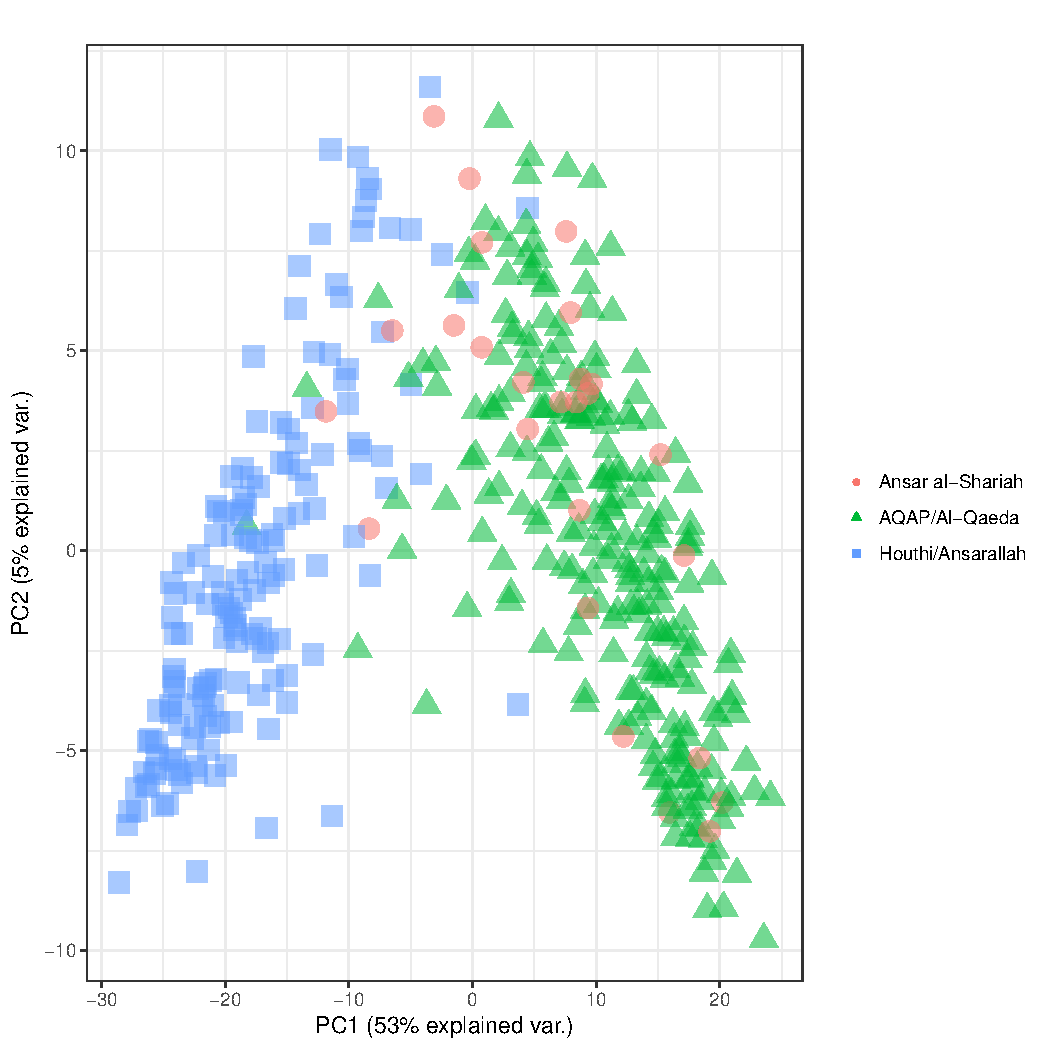
\includegraphics[width=5.00in]{./Pictures/pca_proximityRF.pdf}
\end{tabular}
\caption{PCA Visualization of Group Classification}
\label{fig:rf-pca}
\end{center}
 \end{figure}

%% Move to appendix b/c don't talk about SVM results in body of text.
%%The increasing uncertainty over time in the SVM classification is likewise ambiguous as the result largely derives from mispredicting AQAP-Houthi pairs.\footnote{Results are similar for a classification carried out on a subset of the corpus comprising just AQAP and Ansar al-Shariah stories.}

The clustering analysis is suggestive of convergence in reporting on activities of AQAP and Ansar al-Shariah. However, these methods do not adjudicate between competing explanations for the similarity. Potential reasons for the lack of differentiation include AQAP acting like Ansar al-Shariah; Ansar al-Shariah acting like AQAP; or the algorithms identifying shared features other than underlying behavioral similarity. Moreover, the news classification approach does not directly measure activity. In evaluating the style and coverage of third-party reporting, the results are sensitive to descriptive idiosyncrasies. For example, given the international salience of the al-Qaeda name, the news corpus likely contains over-attribution to AQAP. Similarly, under-attribution of Ansar al-Shariah activities can be introduced by journalists associating AQAP and Ansar al-Shariah.\footnote{Notably, 11 of the stories in the corpus carried language that blurred the distinction between AQAP and  Ansar al-Shariah. For example, an article from Xinhua News stated: \say{Al-Qaida in the Arabian Peninsula, also known locally as Ansar al-Sharia.}}  This may be a result of journalists including more contextual discussion as the security situation unraveled, thus dedicating article space to similar content. Alternately, the increased conflation of AQAP and Houthi stories may pick up a tendency of writers to frame AQAP mobilization using the rebellion frame that dominates coverage of Houthi activities.

\subsection*{Direction of Convergence}
\label{sec:direction-convergence}

A second approach to using text data as a window into opaque organizations leverages topic models applied to materials issued by the groups themselves. To adjudicate the possible direction of convergence in descriptions of AQAP and Ansar al-Shariah activity, I use the Structural Topic Model to summarize changes in latent topics within the corpus~\autocite{roberts2014stm}.  The model is well suited to addressing questions of convergence as it permits modeling group-level changes in attention over time by incorporating document-level information as a covariate related to topic prevalence. Existing work has applied the STM to a variety of corpora similarly comprised of short and moderate-length documents~\autocite{roberts2014structural}, such as open-ended surveys~\autocite{tingley2017rising}, social media messages~\autocite{bail2016cultural}, and deepweb forum posts~\autocite{munksgaard2016mixing}.

\subsection{Communique Analysis}
\label{sec:communiques}
To address the question of the direction of the apparent convergence of
AQAP and Ansar al-Shariah behavior, the following section presents
selected results from three Structural Topic Models estimated on AQAP
and al-Qaeda Central propaganda releases, showing a general
localizing trend in AQAP's self-presentation.\footnote{The Technical Appendix
  features information about text processing and a fuller
  characterization of the results.} The following analysis interprets rising prevalence of Yemen-specific topics and decreases in transnational and pan-jihadi topics as suggestive of an influential parochial base. The timing and content of any change in self-presentation can shed light on the question of whether the topic models reflect underlying ground truth: although communiques and speeches do not necessarily align perfectly with ground truth, finding that themes in AQAP self-presentation move along with the convergence in stories about AQAP and Ansar al-Shariah should bolster confidence that each technique is picking up a real change.

The analysis was conducted on a corpus of 875 documents released by al-Qaeda in the Arabian Peninsula from June 18, 2004 through September 18, 2016.\footnote{The corpus includes content from both the current--\textit{i.e.} post-2006--- AQAP and a predecessor organization of the same name that is occasionally referred to as al-Qaeda in Saudi Arabia.  AQAP is a direct successor to the Saudi Arabian-based \say{AQAP}, and the Yemen-based AQAP leadership actively sought to present the organizations as linked entities. Therefore, I allow the AQAP corpus to accommodate both the current Yemeni-based AQAP and the earlier Saudi-based \say{AQAP} as this permits examination of the impact of the upswing in drone casualties in 2009 and 2010.} The corpus consists of English translations of documents originally released in Arabic and, occasionally, the original text of English-language releases.\footnote{A very small portion of the
  documents, such as individual articles from \textit{Inspire Magazine}, were distributed in English.} These documents were collected and translated by the SITE Intelligence group, a private research organization that collects and translates jihadi media.\footnote{SITE Intelligence Group translations are advantageous for this project, as the company maintains near real-time coverage of prominent online distribution sites and has internal procedures to ensure consistent translation in style and tone.} As no official universal archive of AQAP's releases exists in the public domain,  the corpus is necessarily a sample of the releases. However, as the SITE Intelligence Group is an internationally-focused monitoring
  organization, any systematic selection effects should bias the results against finding increased local self-presentation because bias could be expected to prioritize documents intended for an international audience which should then carry an internationalist message.
  
Official releases are an attractive source of information about changing organizational priorities because, within certain ideological constraints, these documents
provide a forum on which an organization can choose how to
frame their self-presentation. As well, the technological environment makes propaganda documents appealing in this context: since 2011, online platforms have been a \say{major means of communication} within
Yemen~\autocite[33]{carapico2014yemen}. This implies that media distributed online can be consumed by domestic as well as international audiences. The two-level audience can be expected to discourage AQAP from strategically differentiating their online
signaling from their local self-presentation. Readers may worry that even if online platforms are important for communication in the country, Yemen's relatively low internet penetration rate may imply that AQAP's online propaganda is not intended for a domestic audience. If this the case, it should likewise bias the results against findings in support of the bottom-up localizing hypothesis.\footnote{As well, one may be concerned that a strategic actor could use in-person networks to signal which documents are intended for local versus international audiences. However, the difficult information and security environment in Yemen makes it risky to rely on a bifurcated media strategy.} 
The first model addresses the question of direction of convergence in third-party reporting about the activities
of AQAP and Ansar al-Shariah. The outcome predicted by the bottom-up theory of organizational change
expects that an influx of fighters was followed by AQAP adopting a
more local, Yemeni-centric, self-presentation. A second model addresses the counterfactual that regional  and global developments may account for changes in AQAP messaging, independent of any changes in membership base. To account for the possibility that observed shifts in messaging were driven by top-down directions from al-Qaeda leadership or general trends in the jihadi environment, the model contrast the rhetoric of AQAP with that
featured in an additional 500 documents released by as-Sahab, a media
production house closely associated with al-Qaeda's senior leadership.  Finally, a model that evaluates the differences between AQAP's presentation of their \say{Ansar al-Shariah} and the main AQAP branding can be found in the Technical Appendix. This model verifies the operating assumption AQAP's propagandists sought to depict Ansar al-Shariah as the more locally-involved Sunni militant group.

\underline{Model: Evolution of AQAP Messaging}\\

The first model characterizes the evolution of AQAP messaging across the 875 documents in the corpus in order to evaluate trends in the
thematic content of AQAP's messaging.  The bottom-up transformation
theory described above predicts that an influx of local
recruits should encourage AQAP to adopt increasingly local
priorities, and thus that convergence in third-party media coverage of
AQAP and Ansar al-Shariah should be driven by changes in AQAP.  If, as
argued above, organizational messaging tracks true organizational
priorities, changes in AQAP's focus should manifest in the topic model
identifying an increased prevalence of themes relating to domestic fissures, such as the Houthi-Sunni civil war, and a decline of transnational themes. 

Although general trends alone are unable to directly test the predictions of the bottom-up transformation theory, relative differences in the proportions of themes can indicate the general plausibility of the argument. In the
case of Yemen, the theory predicts that increased access to local
recruits should drive AQAP to adopt an increasingly localized
agenda. If AQAP is increasing attention to domestic considerations and themes, the localizing trend suggests that changes in AQAP are driving the difficulty in classifying AQAP and Ansar al-Shariah's activity.\footnote{Analysis of the differing ways in which AQAP presents itself in communiques released under the AQAP and Ansar al-Shariah "brands" can be found in the Technical Appendix.}

Attention within the AQAP corpus is modeled via an 18-topic structural
topic model.\footnote{For discussion of model specification, see the accompanying Technical Appendix.} The topics are presented in Figure~\ref{fig:topicSumsED}, clustered into four thematic groupings: locally-focused war reports, discussions about and threats of clandestine operations, topics promoting transnational jihadi sentiments and goals, and jihadi-associated descriptors. Within each cluster, topics are summarized by their FREX words, which are words or tokens that are associated with the topic but relatively unlikely elsewhere in the corpus. Figure~\ref{fig:EDModelTopicProportions} shows what proportion of the entire corpus of communiques is expected to be assigned to each of the fifteen substantively interesting topics.\footnote{The three remaining topics relate to the construction of the documents themselves, and are less interesting as a reflection of AQAP's self-presentation. These topics relate to videography, habitual sign-off terms, and transcript production.}  As the figure indicates, when the entire corpus is taken together without any disaggregation by document release date, the two most common topics are relate to the Houthi militias and terms that describe local targets and operations. From there, a number of topics that associate words around ideological and tactical themes are each expected to feature in about 10\% of the total documents.

\begin{figure*}
\begin{center}
  \caption{Groupings of Substantive Topics in General Trends Model}
  \label{fig:topicSumsED}
  \begin{tabular}{cc}
 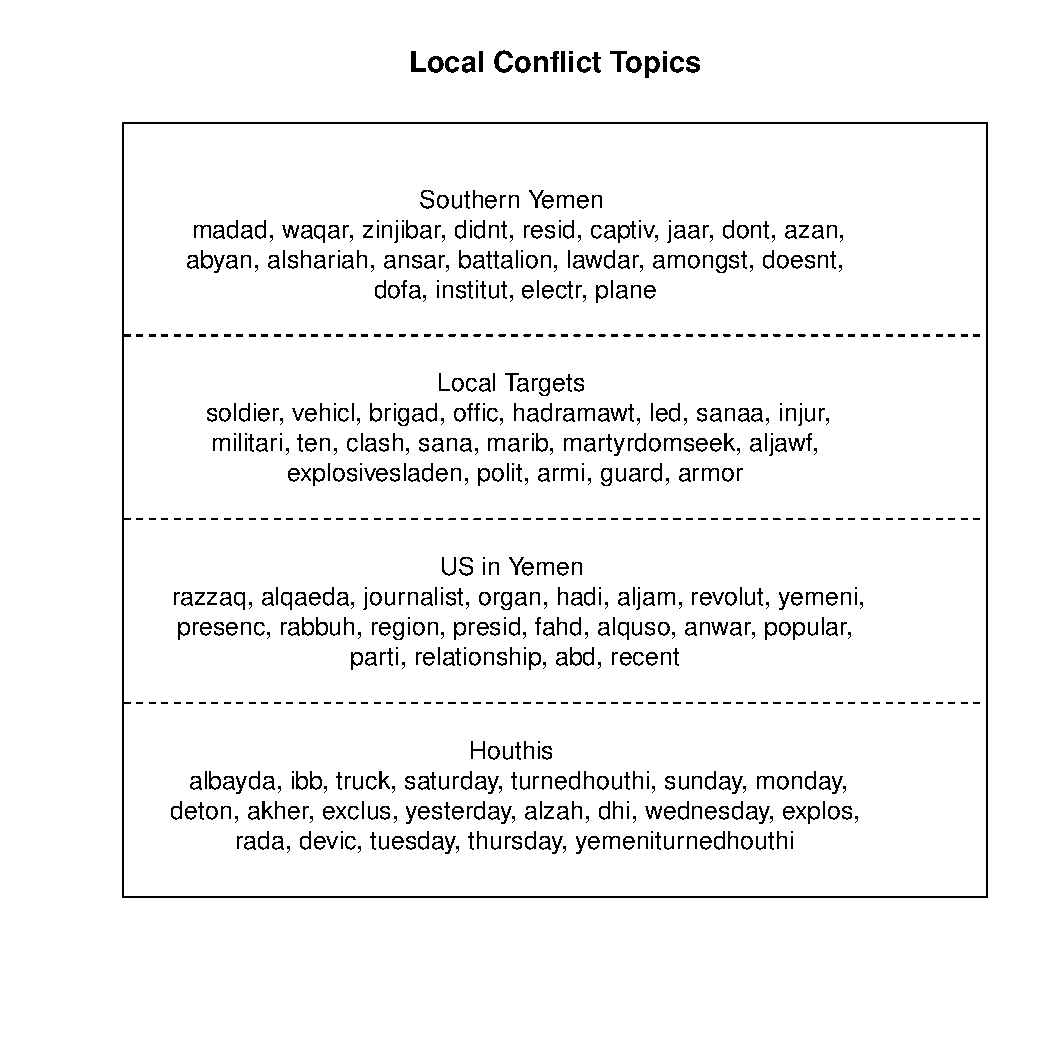
\includegraphics[width=.49\columnwidth]{./Pictures/dayModel_UT70_cluster1.pdf}&  
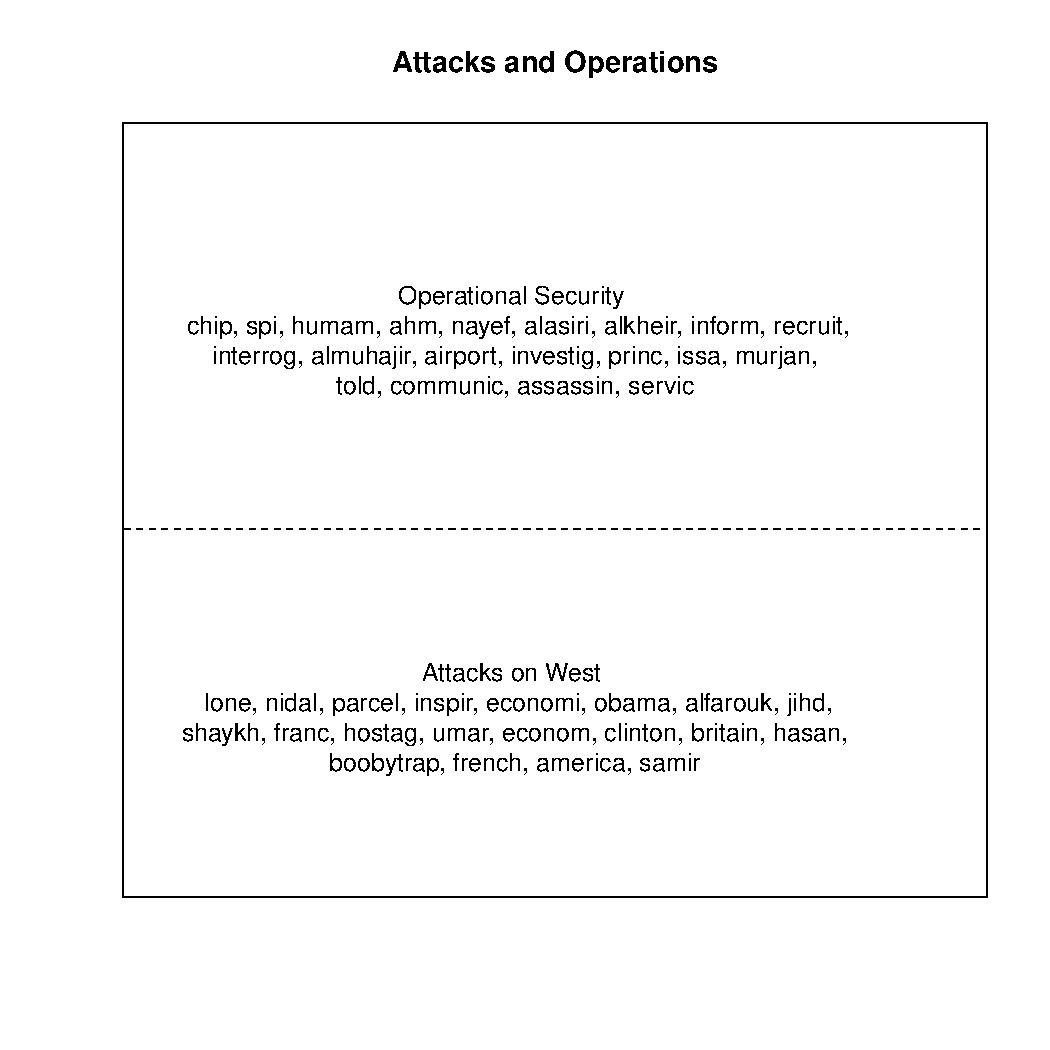
\includegraphics[width=.49\columnwidth]{./Pictures/dayModel_UT70_cluster2.pdf}\\
\vspace{-1.00cm}
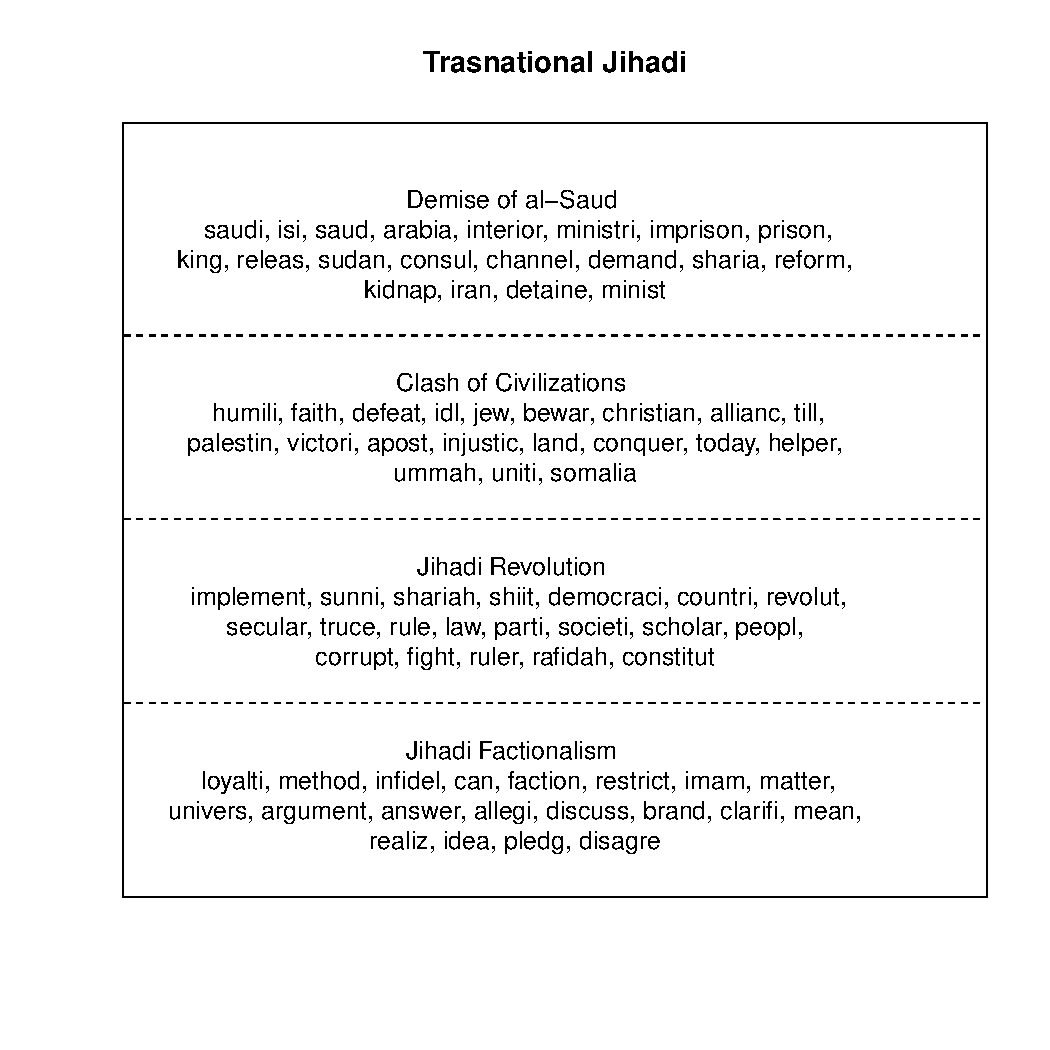
\includegraphics[width=.49\columnwidth]{./Pictures/dayModel_UT70_cluster3.pdf}&  
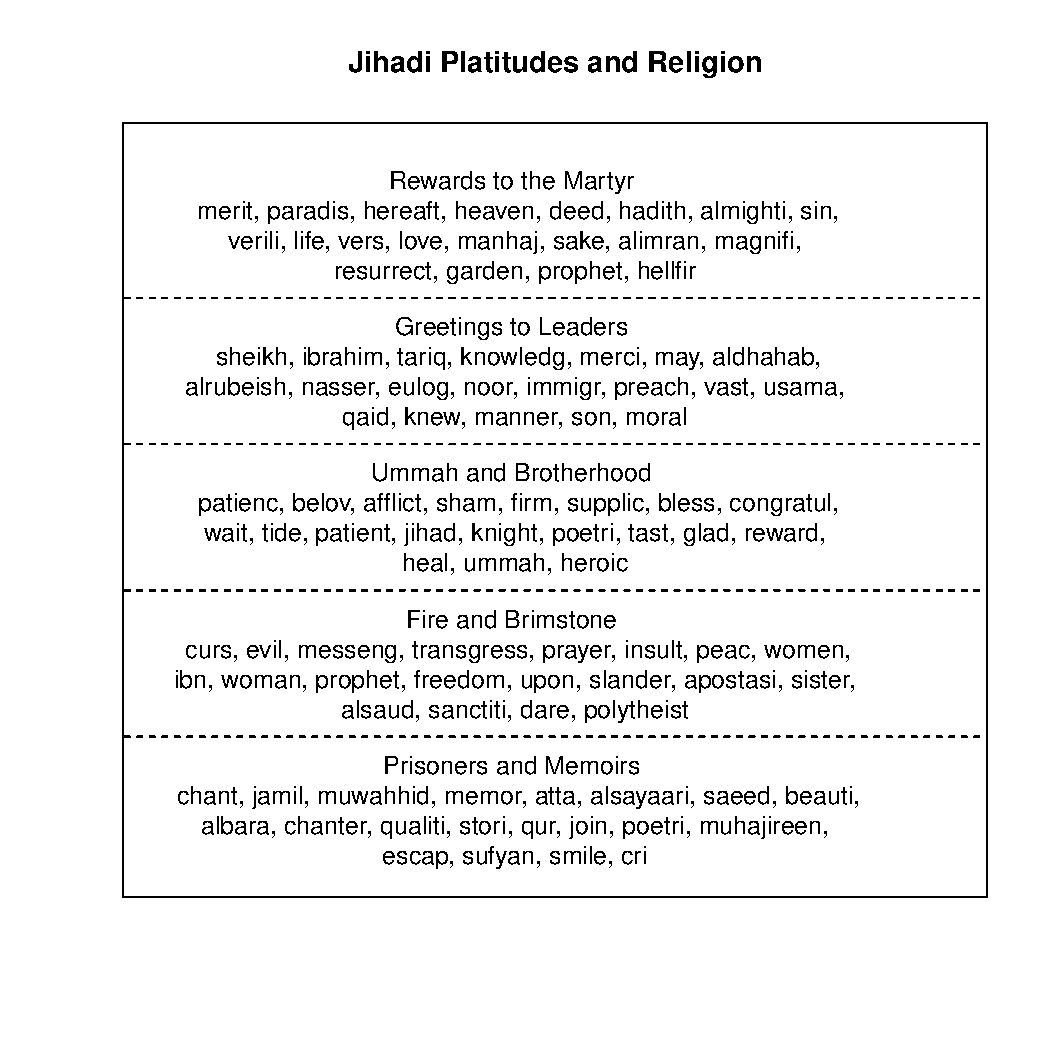
\includegraphics[width=.49\columnwidth]{./Pictures/dayModel_UT70_cluster4.pdf} \\
  \end{tabular}
\end{center}
  \end{figure*}

\begin{figure*}
  \begin{center}
  \begin{tabular}{c}
    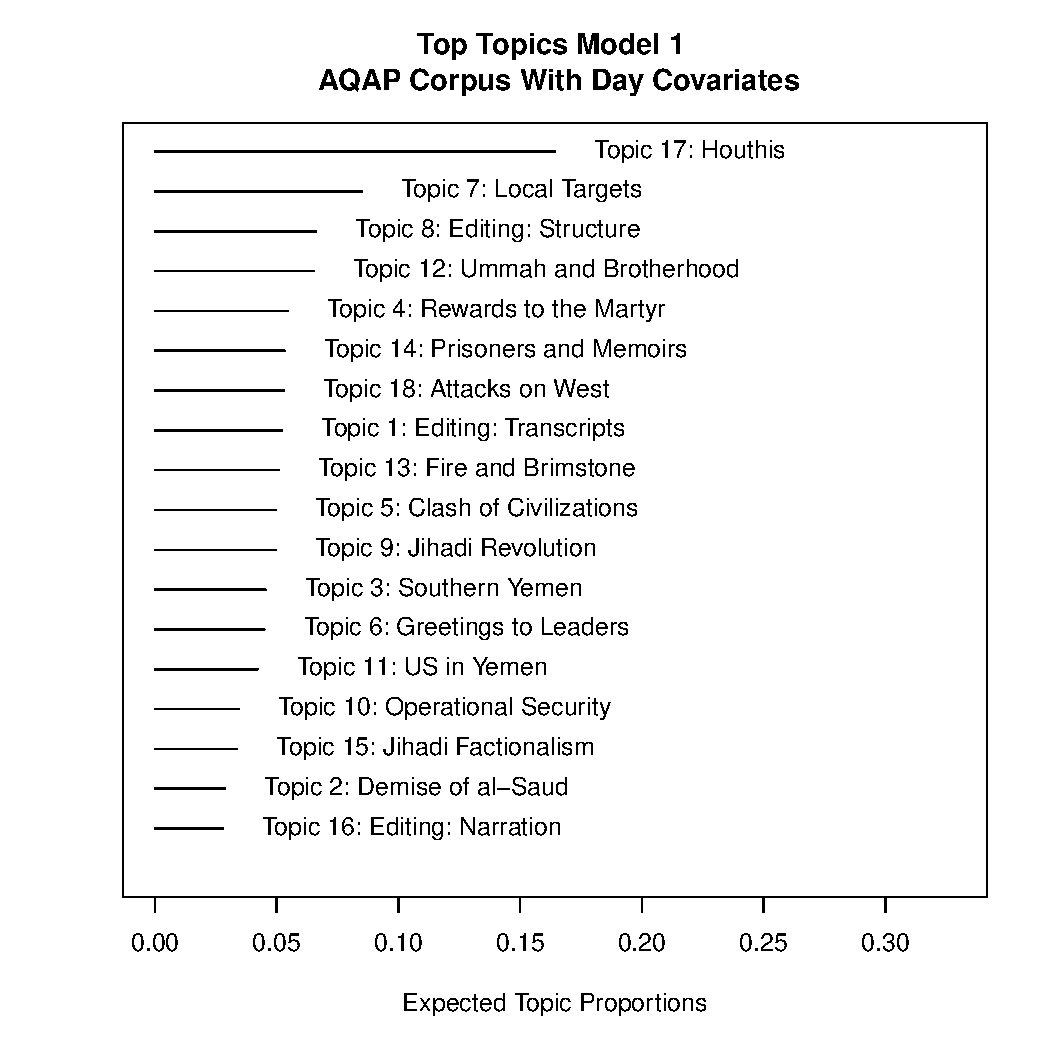
\includegraphics[width=4.00in]{./Pictures/topicProportions_UT70EDModel.pdf}\\
  \end{tabular}
  \caption{Estimated Topic Proportions in al-Qaeda in the Arabian
    Peninsula Corpus}
  \label{fig:EDModelTopicProportions}
\end{center}
\end{figure*}

The relative frequency of topics specifically about Yemen provide the
first place to look for evidence of a local trend in AQAP's messaging. As several of the thematic clusters identified by the model relate to various facets of AQAP's activities in Yemen---including discussion of Houthi militants, activities in Southern Yemen, castigation of the Yemeni government, and descriptions of local operations--- combining the estimated prevalence of each Yemen-centric topic gives an easily-visualized overview of the changing salience of local concerns in AQAP propaganda output. Figure~\ref{fig:l-t-clusters} depicts the expected document-level topic
proportion for the \say{Local Conflict} cluster. The cluster is characterized by words that refer to specific local operations, geography, and political jurisdictions.  Indeed, documents representative of this topic are often battlefield communiques issued to claim local
territorial control. Even the most transnational of the topics, the
\say{US in Yemen} topic, emphasizes political events in the country.
Thus, document space dedicated to each of the \say{Local Conflict}
topics reflects a prioritization of domestic Yemeni issues over
transnational themes. Furthermore, a localizing trend is underscored by looking at changes in the expected prevalence of the four topics that speak to a transnational jihadi sentiment. These topics refer to regional power centers, notably the government and security apparatus of Saudi Arabia, and social concerns that are typical of the transnational jihadi movement. Taken together, the prevalence of these four topics begins to decline from a peak in late 2012, as AQAP's propaganda becomes increasingly focus on the local Yemeni civil war.\footnote{Readers might be concerned that the inverse relationships between topic proportion allocated to the \say{transnational} and \say{local conflicts} are simply mechanical. Although the total prevalence assigned to all topics in the model does sum to one, and thus increased attention to one topic necessarily means less attention to others, the \say{transnational} and \say{local
conflicts} clusters never exceed an expected topic percentage of 75\%
of any given document. Moreover, the mean expected topic proportions dedicated to the two topics is 45\%. Thus, the two topics could co-exist if desired by AQAP's propagandists.}

\begin{figure*}
\begin{center}
\begin{tabular}{c}
  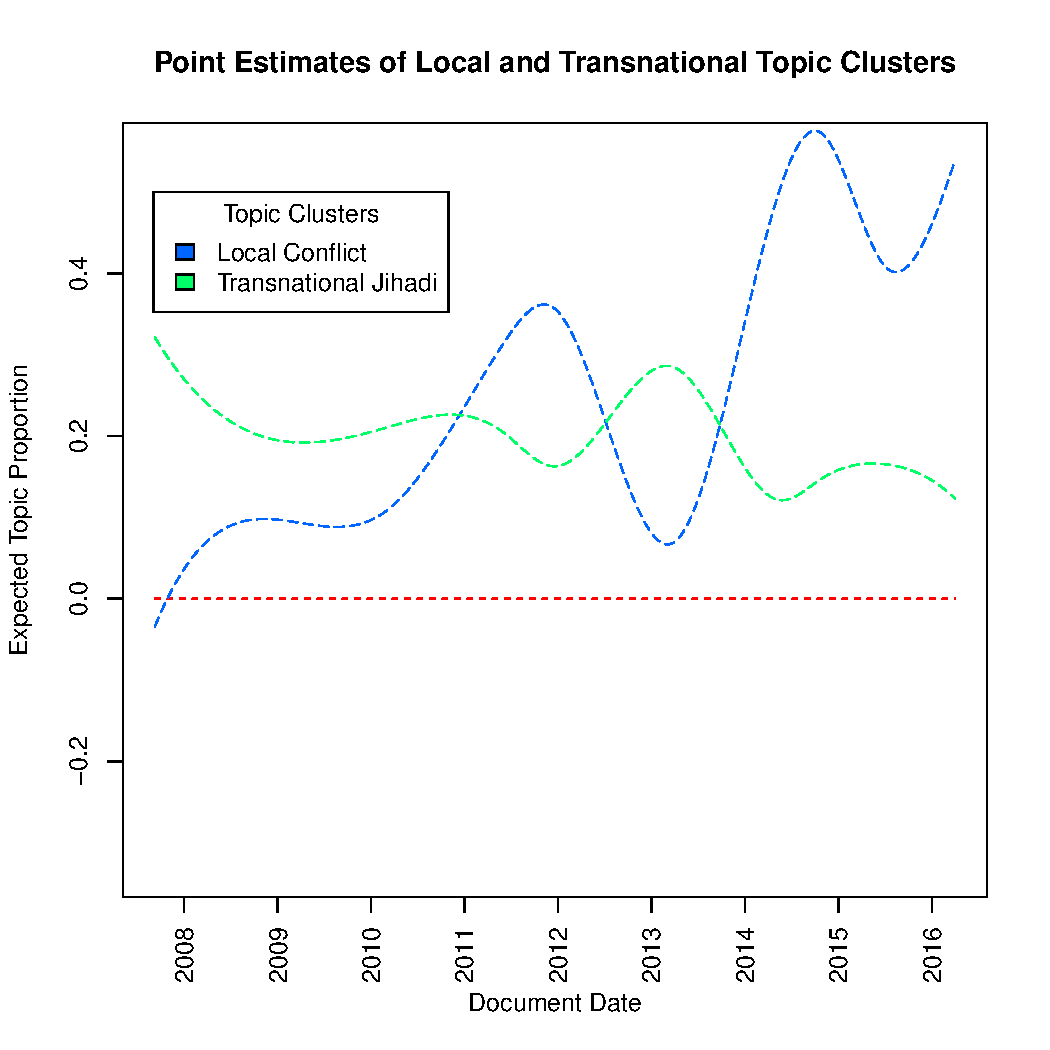
\includegraphics[width=5.00in]{./Pictures/localtranscluster.pdf}\\
\end{tabular}
\caption{Changes over time to attention dedicated to local and transnational themes }
\label{fig:l-t-clusters}
\end{center}
 \end{figure*}

\subsection{Comparison to Central al-Qaeda Messaging}
\label{sec:STM3}
Thus far, the analysis has suggested that local observers generally
characterized AQAP and Ansar al-Shariah using similar terminology and
framing, and despite investment in Ansar al-Shariah as the local face of the movement, AQAP's communiques become progressively
more local in theme.  Although these results are generally
consistent with the theory's expectation that an influx
of local fighters generated internal pressure on AQAP to focus on
local issues, an alternate explanation could point to broader forces
among the transnational jihadi community. In particular, 2011, the year of
the Yemeni Revolution, also saw a series of shockwaves through the
jihadi world after Usama bin Laden was killed on May 2, 2011. His second in command,
Ayman al-Zawahiri, subsequently assumed leadership of the global
al-Qaeda network. In September of that year, an American drone strike
killed Anwar al-Awlaki, an American-Yemeni cleric who had been a
strident internationalist face for AQAP.

The deaths of bin Laden and Awlaki, and Ayman al-Zawahiri's subsequent
ascendance to the leadership of al-Qaeda, are challenging for the theory
developed above. Al-Zawahiri has long been associated with an
internal al-Qaeda faction that prioritizes focusing on implementing
country-specific social and political revolutions in the home
countries of al-Qaeda's operatives, rather than engaging in
civilizational struggle against the American-lead global
system~\autocite[147]{miller2015audacious}. Correspondingly, Awlaki was
instrumental in AQAP's efforts to radicalize and mobilize fighters
internationally, particularly from the West.

Thus, one possible counter-narrative to the bottom-up transformation
argument maintains that the change in al-Qaeda's leadership may have triggered a wider ideological shift that filtered to local branches and that Awlaki's death amplified
the effect in Yemen. Indeed, if AQAP was following the lead of al-Qaeda Central after 2011, changes in AQAP's self-presentation would not be informative about the grassroots transformation theory.

To differentiate a local change in Yemeni rhetoric from changes prompted by a top-down al-Qaeda strategy, this section presents selected results from a structural topic model that estimated topic prevalence in a corpus of propaganda released by AQAP and as-Sahab, al-Qaeda's central media wing.  AQAP's changing rhetorical style is presented alongside that of as-Sahab to establish that observed changes in AQAP rhetoric are not driven by an underlying pan-jihadi trend. This model, Model Two, identified themes in a corpus of 1375 documents, of which 875 were AQAP communiques and 500 were  releases from as-Sahab. The model predicted topic prevalence as a function of time interacted with whether the document was authored by AQAP or as-Sahab.\footnote{Time is included in this model as a linear function for computational tractability.}

The patterns are generally intuitive: overall AQAP is more likely to talk about
Yemen-related topics while topics that discuss other battlegrounds and
targets for revolution are more associated with as-Sahab.\footnote{A
  full analysis is discussed in the Technical Appendix} However, the
divergence in thematic prevalence of pan-jihadi topics between
releases issued by as-Sahab and AQAP indicate that AQAP's increasing
Yemen focus was not indicative of a localizing turn lead or directed
by al-Qaeda Central, via their as-Sahab mouthpiece. Two such themes are highlighted below. The two highlighted themes were chosen for their popularity among globally-minded jihadis. The first is characterized by an explicitly transnational list of FREX words: it features countries with active jihadi battlegrounds as well as references to what jihadis perceive as an American-Israeli alliance against Muslims around the world. The second topic is a relatively abstract transnational theme that attempts to mobilize jihadi supporters by referencing vulnerable demographics of Muslims, such as women and children, experiencing hardship and travails.

Figure~\ref{fig:crusaders} highlights two topic outcomes from the model.  The first topic is analogous to both of the \say{Clash of Civilizations} topics above, here titled  \say{Crusaders and Zionists.}\footnote{As a different model, the topics are unique to this model although generally similar to the themes from Models One and Two.}  This topic is notable for having a strong transnational jihadi focus; exactly the type of subject that AQAP should cease to discuss if their domestic recruitment is
driving a local focus. Indeed we see that although al-Qaeda Central's
rhetoric does increasingly feature this topic, AQAP becomes
progressively less and less inclined to use words associated with the
topic. Interestingly, AQAP's move away from the ``Crusaders and
Zionists'' topic occurs even though AQAP documents were originally more likely to feature the topic than were as-Sahab documents.

Similarly, after 2011, as-Sahab documents become more likely to
discuss a topic addressing alleged injustices against vulnerable
populations such as women and children. The topic, which I name ``Defending
the Weak,'' expresses indignation about alleged crimes against Muslim
women and children and is a pervasive theme of transnational jihadi
rhetoric. Throughout the time period covered by the corpus, the topic
becomes less common in AQAP documents and more prevalent in as-Sahab releases. 

\begin{figure*}
\begin{center}
  \caption{AQAP and as-Sahab Divergence}
  \label{fig:crusaders}
  \begin{tabular}{cc}
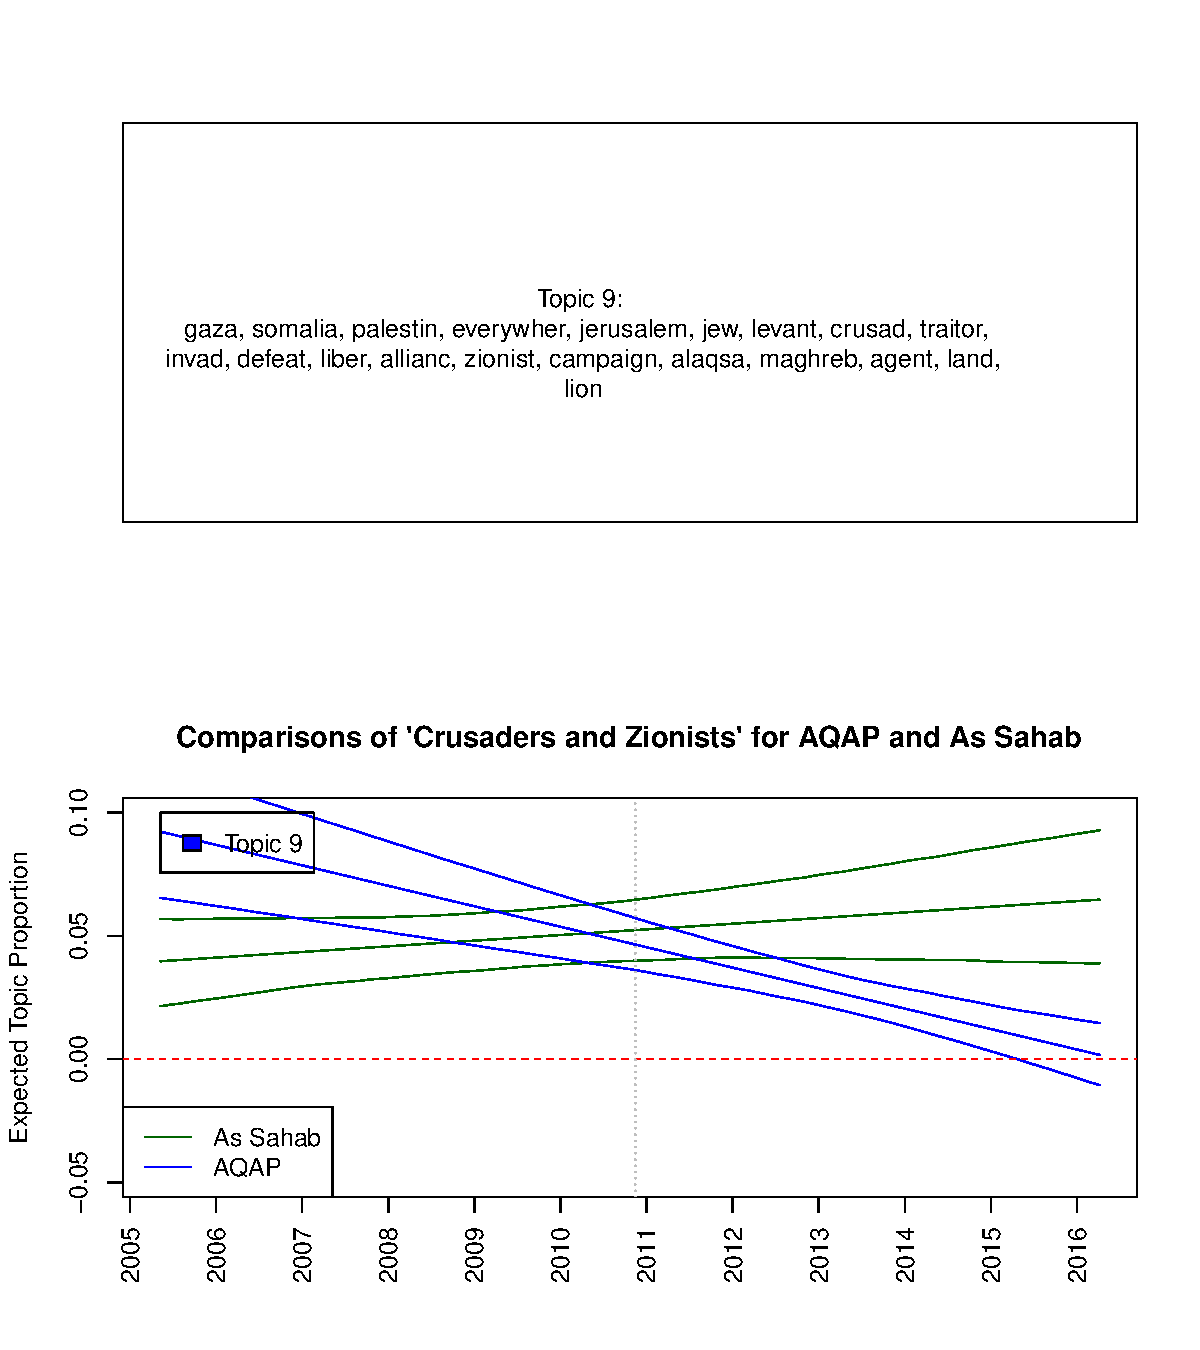
\includegraphics[width=.45\columnwidth]{./Pictures/34TopicsComparisonCrusaderZionists2.pdf}&
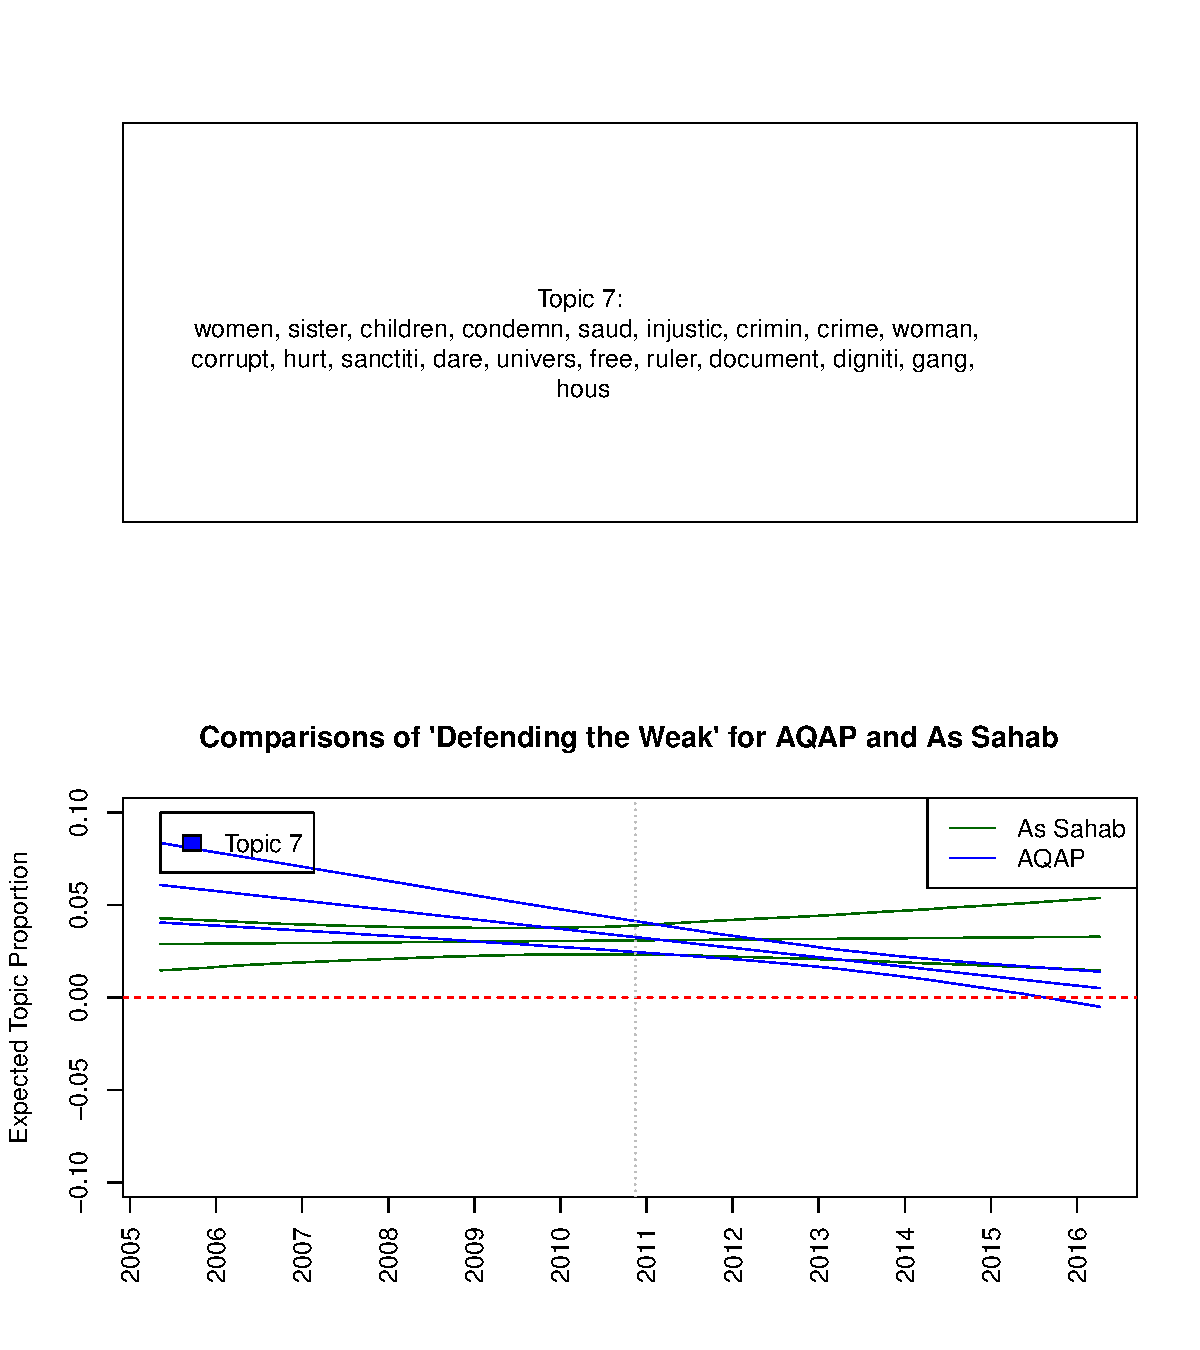
\includegraphics[width=.45\columnwidth]{./Pictures/34DefenseofWomen.pdf}\\
  \end{tabular}
\end{center}
 \end{figure*}
}
\chapter{Portability of the Personnel Resource Curse Theory}
\label{chap:survey}
 
Previous chapters have introduced a theory of how the preferences of upward-driving pressure for organizational change in which the grassroots can reshape an organization by constraining the ability of leaders to dictate strategic goals. The theory predicts that an organization would be susceptible to bottom-up transformation when three conditions are present: (1) heterogeneous preferences of the leadership and rank-and-file, (2) restricted ability or desire to titrate the inflow of new members, and (3) labor mobility among the rank-and-file.  Thus, far the manuscript has primarily explored the implications of the theory for the operation and trajectory of militant organizations. In the chapter that follows, I argue that analysts should find evidence of the Personnel Resource Curse and upward-driving transformation in an entirely different domain: that of licit mission-driven organizations. Although many types of licit organizations can be considered to be mission-driven, I particularly focus on the non-profit sector as this sector shares important similarities with the militant groups. 

To motivate the extension into this domain, I begin the chapter with an analysis of the similarities between the challenges of managing a non-profit organization and those faced by leaders of militant groups.  I then turn to an original survey of managers and directors of non-profit organizations to demonstrate that recruitment patterns that contribute to the Personnel Resource Curse are relatively common for issue-motivated groups, as is reported experience with bottom-up transformation. Finally, I present the results of a factorial experiment designed to test the intuition that financial incentives can encourage these leaders to hire personnel who do not share their organization's mission. I find that while a substantial number of the respondents agreed that they had experienced recruitment of non-aligned members, when presented with a choice experiment, respondents answered that they were willing to exchange financial incentives for mission cohesion. This result suggests that survey respondents attempt to avoid situations that might initiate a membership-driven mission drift.

\section{Motivation for Extension}

At the core of the accommodation theory is a general claim that leaders behave in a non-optimal way: they recruit beyond their socializing capacity. This recruitment behavior drives the counter-intuitive predictions of the theory: when successfully ensuring the continued operation of their group through recruitment expansion sets the organization on a course that will take it away from the leader’s preferred trajectory. In particular, the theory predicts that the recruitment pattern that drives the bottom-up transformation process can occur with the foreknowledge of the leader but being directly initiated by them.

The previous case narratives indicate that this behavior can be found among militant and underground groups. However, armed groups operate in consequential, but unique contexts. Moreover, their decision-making is often deliberately hidden until after the conflict has resolved or the individual is no longer a participant. This opacity means that much of the data used earlier is retrospective or identified by outside observes, which introduces the possibility that the rapid recruitment behavior and eventual upward pressure are artifacts of hindsight or incorrect conclusions drawn by observers.  

To establish the observation of rapid recruitment, I turn to a population of leaders in an analogous but easier to reach population. In the chapter that follows, I first argue that for the attributes that are significant for the bottom-up transformation theory, there are substantial parallels between the management of militant organizations and that of non-profit organizations. I then introduce a survey of non-profit leaders and managers about their experiences with rapid personnel recruitment.

Non-profit organizations should be a useful case in which to identify whether the bottom-up transformation theory travels because of the emphasis on buy-in, consensus, and inclusive decision-making has a strong implication of a leadership style based on negotiation and accommodation. For example, a former Dean of the UCLA School of Business and The Getty emphasized that non-profit leaders can not rely on fiat or top-down decisions:

\say{You will have little opportunity to lead by making decisions…if you have a vision or you want to make any changes, you're going to do it by leadership and by inspiration and not by direction. You've got to be a Pied Piper.}~\autocite[7]{taliento2005corporate}

The survey focuses on the initial step of the theory: the initial recruitment of relatively large cohorts of new members whose preferences to not align with those of the group's leadership. Yet, as argued in the previous chapters, leaders may face circumstances in which they have a compelling reason to recruit beyond their socializing capacity.

As in the domain of militant organizations, this recruitment and change pattern operates counter to a large body of literature. Scholarship on the determinants of workplace organizational change has primarily focused on the agency of leaders who are typically assumed to create recruitment and management policies that ensure smooth selection and integration of new members~\autocite{barber1998recruiting, kotter2012leading, rynes1989recruitment, kotter2012heart, paglis2002leadership, wanous1992organizational}.  Following Hirschman, an extensive literature by management scholars, political scientists, and sociologists analyze when dissatisfied members of declining firms decide between exiting their groups or attempting \say{to change rather than escape from an objectionable state of affairs}~\autocite[30]{hirschman1970exit}. This insight has given rise to a literature on how employees express dissatisfaction with their companies~\autocite{bjorgo2008leaving, dowding2000exit, farrell1983exit, wilkinson2011new, wilkinson2014handbook, withey1989predicting} although with less attention to how leaders respond~\autocite{liu2010warn} and more emphasis on focuses on moments of acute dissatisfaction with working conditions or organizational quality~\autocite{morrison2011employee}.

\section{Can we compare licit nonprofits and covert militant groups?}

Thus far, I have outlined a process by which the strategic preferences of subordinates begin to become more influential than the strategic preferences of the leader or leadership. The initial framing of the theory is deliberately general. Indeed, the juxtaposition of both licit---non-profit organizations and startups--- with illicit--- militant and terror organizations--- may strike some readers as unlikely or even unprincipled. 

I argue in this section that these organizations are more similar than they may appear to be. I particularly make the case that even the most extreme type of organization, terrorist groups such as al-Qaeda, are subjected to many of the same managerial tensions and trade-offs as their aboveboard counterparts. 

Why should we believe that such disparate types of organizations face similar challenges and are thus comparable?

The most straightforward approach is to turn directly to the practitioners. Popular management advice aimed at the non-profit sector explicitly draws parallels between leading non-profit and for-profit organizations~\autocite{azevedo2018success, gaussndwhy} and the startup investor Y Combinator invites non-profit organizations and socially beneficial \say{B Corporation} firms to compete for funding, noting that the firm \say{treat[s] nonprofit startups almost exactly like for-profits}~\autocite{walker2017what}.

For even the most extreme of the comparisons, between underground revolutionary organizations and licit business, militant strategies report facing general organizational challenges that would be recognizable to a start-up CEO. Indeed, an influential jihadi strategy guide, \say{The Management of Savagery,} directly analogizes clandestine and revolutionary groups to aboveboard organizations.  In presenting his method for imposing the supposed political and social systems of early Islam into the current world, Abu Bakr al-Naji, tells his readers to seek out popular management books:

\begin{quote}
We  must  make  use  of  books  on  the  subject  of  administration,  especially  the  management  studies and theories which have been recently published, since they are consonant with the nature  of  modern  societies.    There  is  more  than  one  site  on  the  Internet  in  which  one  can  obtain management books. .... Moreover,  it  is  possible  to  obtain  more  management  books  and  resources  from  other sites on the Internet or from libraries and publishing houses, keeping in mind that we must undertake practical application when study of them is complete so that we may see the administrative styles (positively) influence the work. \autocite[56]{mccants2006translation}
\end{quote}

Beyond what practitioners themselves say, scholars have identified other facets of terror and militant functioning with clear parallels to the aboveboard business world~\autocite{mironova2019freedom, shapiro2013terrorist}. Other scholars have successfully applied tools developed to predict the trajectory of business startups to similarly predict which emergent terror groups will become more successful~\autocite{yang2019quantifying}.

%% I probably need a few line about why I can treat many different types of organizations ad being subjected to similar dynamics. Can probably point to . Shapiro, Crenshaw on why to connect even two apparent extremes (military and clandestine revolutionary orgs)

\subsection{Similarities}

It may seem that armed militant organizations and non-profit organizations should occupy two vastly different worlds. The former raises images of masked fighters brandishing weapons in the bed of a Toyota Hilux truck or holed up in urban battlegrounds. Conversely, the later is more associated with well-meaning organizers marshaling volunteers to tackle social problems on a shoestring budget.\footnote{Just as the category of \say{militant group} covers a wide range of organizations of widely varying size, resource endowments, and precarity, the \say{non-profit} sector covers a vast range of organizations. The sector encapsulates everything from a tiny organization bootstrapping on an operating budget that allows for only a single staff member to university and hospital systems that are some of the largest employers in their respective states. In both cases, large, highly institutionalized organizations with stable resources and funds are the minority~\autocite{cunningham2013non, frailey201looklike} Size influences institutionalization and socializing capacity. The argument presented here would expect that in both domains, large and well-institutionalized organizations with high socializing capacity and the resources to be able to select personnel carefully should experience this type of transformation less frequently, if ever.} Yet, as I outline below, there are many structural similarities that suggest that the bottom-up transformation theory should apply to non-profits in similar ways as for militant groups. 
 
% 1- Militant groups not sui generis

Although managing violence, and particularly managing violence under the threat of repression, heightens the challenge of management and delegation and sets up novel challenges~\autocite{della2013clandestine, oots1986political, shapiro2012moral}, analysis of militant and violent clandestine groups often makes an explicit comparison and reference to the characteristics shared with licit organizations. The organizational and managerial parallels have been elaborated across an array of domains, including al-Qaeda's franchise strategy, formal human resources policies, and principle-agent and internal management dilemmas~\autocite{berman2011can, byman2010agents, crenshaw1987theories, cunningham2013actor, dtr2011papertrail, eid2017french, farrall2011qaeda, hoovergreen2016, nwajiaku2012political, salehyan2014external, shapiro2012terrorist, shapiro2013terrorist, skaperdas2002warlord, tamm2016rebel,wright2006looming, zaw2017hr}. Similarly, the literature on the political economy of organized crime has drawn similar parallels between grey and black market organizations and aboveboard organizations~\autocite{cappellaro2020maintaining, leeson2007arrgh, skaperdas2001political, skarbek2011governance, sullivan2002drug}.  The distinctive organizational attributes of militant groups can be expected to strengthen the pathways through which the bottom-up-transformation presented here works, but not render the transformation process unique to armed movements.\footnote{More difficult recruitment environments and increased literalness of the \say{survival} threat should increase the speed at which the leaders accommodate. Counter-balancing these factors that amplify the pathways for bottom-up transformation is that militant groups have advantages in socialization because they can more easily monopolize the attention and contacts of their recruits. They can also make exit a more difficult option, thus reducing the leader’s need to accommodate.}

A survey of experiences of about a dozen business leaders who transitioned into the non-profit sector highlighted several domain-specific idiosyncrasies that leaders in the non-profit sector face.~\autocite{taliento2005corporate} Although intended primarily for leaders transitioning from the for-profit corporate world, the list of leadership challenges in the non-profit sector underscores the reasons to expect the bottom-up transformation theory to also be particularly visible in the non-profit sector.

The report described five areas that highlighted the complexity of non-profit leadership: (1) decentralized authority and control; (2) a wide range of stakeholders; (3) difficulty using metrics to monitor performance; (2) an outsized importance for communications and messaging; (5) and building effective organizational structures despite scarce resources and training~\autocite{taliento2005corporate}. Each of these challenges has a direct cognate to the operations of militant groups.

The first challenge, decentralized authority and control, is one that is directly faced by militant leaders, for many of the same reasons articulated by the surveyed non-profit leaders. In explaining the relative lack of deference, the CEO of the J. Paul Getty Trust noted that a culture in which individuals have more loyalty to the profession than the organization means that they are less likely to be deferential to the nominal leader.  Closely related is the observation that non-profit leaders must have a \say{much more consultative, inclusive decision-making style.} Thus, in terms of the bottom-up theory, lack of automatic deference should be expected to reduce the leader’s expectation of their socialization capacity and should expect more accommodation to the preferences of the base.  These observations have close analogies to the role of militant groups, whose leaders are often managing factions and units that are closely interwoven with pre-conflict social networks~\autocite{staniland2014networks}.

 The third challenge of managing nonprofits, difficulty in generating fine-grained metrics on activities has a direct analogy to the operation of clandestine and decentralized militant organizations~\autocite{shapiro2012moral, taliento2005corporate}. This should heighten susceptibility to bottom-up transformation by making oversight more difficult but does not change the underlying dynamics.  
 
 The second and fourth challenges of managing non-profit groups are two aspects of an intertwined issue for militant operations: more stakeholders creates larger and more complex needs around group messaging and outreach. Having a large and diffuse set of stakeholders raises the stakes of messaging~\autocite{bob2005marketing}. In particular, rebel groups are often coordinating internal messaging as well as navigating their relationship with external sponsors and backers, which means that they often have to navigate message coordination to multiple potential audiences~\autocite{jones2019manifesto, szekely2017politics, coggins2015rebel, popovic2017fragile, tamm2016rebel, huang2016rebel}.
 As well, the role of non-profit leader as an externally-facing fundraiser who must engage in complex multi-level communications outreach to motivate both followers and donors without the typical incentives of money or profits is a position that many militant leaders would recognize~\autocite{taliento2005corporate, bob2005marketing}.

Finally, the fifth challenge in transitioning to non-profit organizations, operating under resource constraints, is one of the most dramatic points of similarity between running a militant group and a non-profit organization. For both, it’s often easier to get funding for operations and activities than it is for capacity-building. Secondly, unless they manage to capture material, both militant groups and service-providing non-profits share the general structure that successful operations drain their resources~\autocite{taliento2005corporate}. 

Both types of organizations frequently operate under fiscal and personnel stress, thus making it more likely that managers would feel the need to take advantage of an opportunity for short-term reinforcement at the expense of long-term cohesion. Indeed, descriptions about the logistical and material needs of militant groups can often look remarkably similar to those of non-profit organizations that provide services. For example, in diary entries describing his visits to the Northern Alliance during the Afghan-Soviet War, Masood Khalili enumerated the constant stream of expenses of food, weaponry, and civilian aid, revealing that \say{The expenditure of the northern zone is staggering... Without money it is very hard to push the wheels of war to victory... It is sweet to give your life in the fight for freedom, but it leaves a bitter taste when you see a friend starving on the battlefield}\autocite[129]{khalili2017whispers}.

Khalili's diary entry, written as part of reflections of visiting the Ahmed Shah Massoud's camp in July 1986, captures the sentiments of service providers who face a constant shortfall.  Non-profit organizations also frequently exist on the razor edge of survival.  Notably, a 2018 analysis of the United States non-profit sector found that approximately half had less than one month of financial reserves, while almost ten percent were technically insolvent with liabilities greater than their assets~\autocite{morse2018financial}. A similar 2016 study concluded that less than one-third of US non-profits are \say{financially strong}~\autocite{roberts2016risk}. Not only do they share similar difficulties in generating sufficient operating funds to ensure survival, but both types of organizations also navigate the challenges of accepting donations without being co-opted. 

Indeed, another major similarity between non-profits and emergent militant groups is that although both need funds for operations, most derive the funding streams without being able to promise investors immediate returns.\footnote{This generalization is less true for militant groups operating in resource-rich terrains and who are strong enough to be able to monopolize force in territory that they control and appear either poised for victory or control over a valuable territory. These groups can, and do, seek \say{investors} by offering concessions. The Liberian Civil was is one well-studied conflict in which rebel groups raised revenue by partnering with international firms~\autocite{lidow2016violent}.} %Am I going to need more citations here? IF so, look at the early 2000s literature on resource conflicts. Keep in mind that I'm not looking at looatable resources but explicitly  looking for seed capital. 


\subsection{Differences}

At the same time, non-profit organizations diverge significantly from militant groups. These differences make such organizations an insightful domain in which to test the hypothesis that leaders can be driven to accommodate the preferences of their base at the expense of their strategic vision.   Most importantly, non-profit organizations differ from militant groups in that they are rarely clandestine or operate in opposition to security forces. Being licit allows them to delegate internally, institutionalize, and professionalize in a way that all but the most stable militant groups have difficulty accomplishing, as robust networks of hierarchy and command introduce vulnerabilities. Professionalization and increased oversight could be expected to provide more leverage to leaders, as they can draw on extensive management guidance and advice that presupposes the leverage and cultural expectations afforded to workplace leaders.

Along with more opportunities for oversight and consolidation and professionalization of internal management, licit operations---and the existence of an active and vibrant economic sector driven by non-profits --- also implies that organizational exit is easier for frustrated personnel. Thus, seeing accommodation in this group of leaders suggests that the threat of exit is even more powerful than countervailing pressure of professional delegation and management. 

\section{Survey Overview}

To investigate whether the non-profit sector is also susceptible to upward-driving pressures for mission change, I surveyed 344 self-identified directors and managers of non-profit organizations about their experiences with growth and recruitment. The survey focused on recruiting new staff for skills, rather than alignment with the organizational mission. The survey, fielded in May 2019, focused on leaders of non-profit organizations because they often operate in a context in which bottom-up transformative pressure is particularly apparent and for the contextual similarities described in the previous section. The sample was collected via the Lucid sampling firm and included respondents who identified as among the top leadership of their respective organizations. Table~\ref{tab:survey1} displays the self-reported roles of survey takers.  In the respondent demographics, the \say{Senior Leadership} category contains those who described their role as \say{Owner, Partner, [or] President} while the \say{Other} category reflects one respondent who identified as Assistant or Associate and an additional nineteen who declined to identify their position.

Using a survey to investigate the degree to which the Personnel Resource Curse theory travels outside of a militant context has several benefits. This strategy trades the potential richness of process-tracing and qualitative cases for a design that can get at two fundamental questions that qualitative and single-case text-as-data approaches are unable to answer: generality and scale. Using a survey can not only indicate whether the personnel resource curse is a theory that travels outside of the domain of militant operations but also provides an estimate of the frequency with which the surveyed leaders do (or do not) experience these challenges.

This insight is particularly valuable in extending the theory outside of militant organizations because getting a sense of the scale at which the Personnel Resource Curse affects armed groups faces a fundamental data challenge. First is the difficulty of estimating the prevalence of recruitment shocks into militant groups for which there is rarely fine-grained, time-series, recruitment data. This not only complicates the tracing of the effects of recruitment shocks into any specific organization but also makes it extremely difficult to develop insight into the universe of potential and actual cases. Second, the internal decision-making of militant groups is often intentionally opaque. Thus, although the militant context is useful for theory development and has application to an operational domain of transnational significance, it is challenging for theory testing.  Conversely, surveying non-profit leaders is conducive to a research design that scales well. It can thus be deployed to many more respondents than are feasible for even a well-researched qualitative team. This permits more insight into the frequency and co-occurrence of the recruitment and accommodation steps of the theory.

Most importantly, the survey asks for reflection both in hindsight as well as of current experiences.  Asking for both helps to avoid the risk that what appears to be leader accommodation is, in reality, mischaracterization to shift the responsibility for contentious or catastrophic decisions.  The risk that instances of bottom-up transformation would be masked by motivated reasoning that caused leaders to change their retrospective characterization of the dynamics is particularly important in cases--such as the militarization of Fatah's Executive Committee after the Battle of Karameh--in which accommodation also made it more difficult for the organization to accomplish its goals in the manner preferred by the leaders.


Of course, relying on a survey is not without drawbacks. Most notably, the survey instrument is not cross-referenced with qualitative interviews or cases, making the results sensitive to widespread misrepresentation.  As well, framing effects are particularly salient for this project: pretesting and interviews conducted as part of the theory development process revealed a strong tendency for leaders to view accommodation as a failure of their role. As a result, they would categorically deny experiencing pressure to respond to the preference of their rank and file and in adjusting their activities to reflect these preferences. Yet, they subsequently acknowledge the utility of accommodation, instead framing the accommodation as a process of responsiveness. Finally, a third advantage of issuing the survey to non-profit leaders is that there is a widely-adopted term, \say{mission drift,} for the concept of an organization shifting away from their original goals.  Thus, the survey was able to rely on this language, rather than introduce a  new, potentially negative, concept and then ask respondents to reflect on their experiences. 

\subsection{Respondent Information}
\begin{table}
\centering
\begin{tabular}{lcc}
Respondent Role  & Total & Proportion\\
\hline
\hline
Manager & 138 & 40\%\\
\hline
Director & 124 & 36\% \\
\hline
Senior Leadership & 53 & 15 \% \\
\hline
Vice President & 8 & 2\% \\
\hline
Other & 20 & 6\% \\
\end{tabular}
\caption{Organizational Roles of Survey Respondents}
\label{tab:survey1}
\end{table}

The respondents appear to have been located throughout the country, responding to the survey from IP addresses corresponding to 45 US states and one Canadian province.\footnote{The five states without associated respondent IP addresses were: Montana, Nebraska, North Dakota, Vermont, and Wyoming. Note that this tally takes the IP addresses at face value and does not systematically investigate the reported IP addresses.} The respondent IP addresses were most concentrated in California (32 respondents), New York (32), Texas (25), Florida (22), Illinois (20), with 20 or fewer respondents from the remaining states. 

The geographic distribution of the IP addresses associated with the respondents is shown in Figure~\ref{fig:surveymap}. As the map indicates, the responses are primarily distributed throughout the Continental United States.\footnote{One respondent, which is not pictured in the map, had an IP address in Alaska.} The IP geolocations are colored by the general issue area reported by the respondent. The distribution of missions does not suggest any systematic sorting of respondents by geographic location.\footnote{The respondents reporting "Other" are predominantly respondents who provided the type of managerial activity that occupies most of their time--- such as staff training, or logistics--- rather than the mission area of their organization.}

\begin{figure}[t]
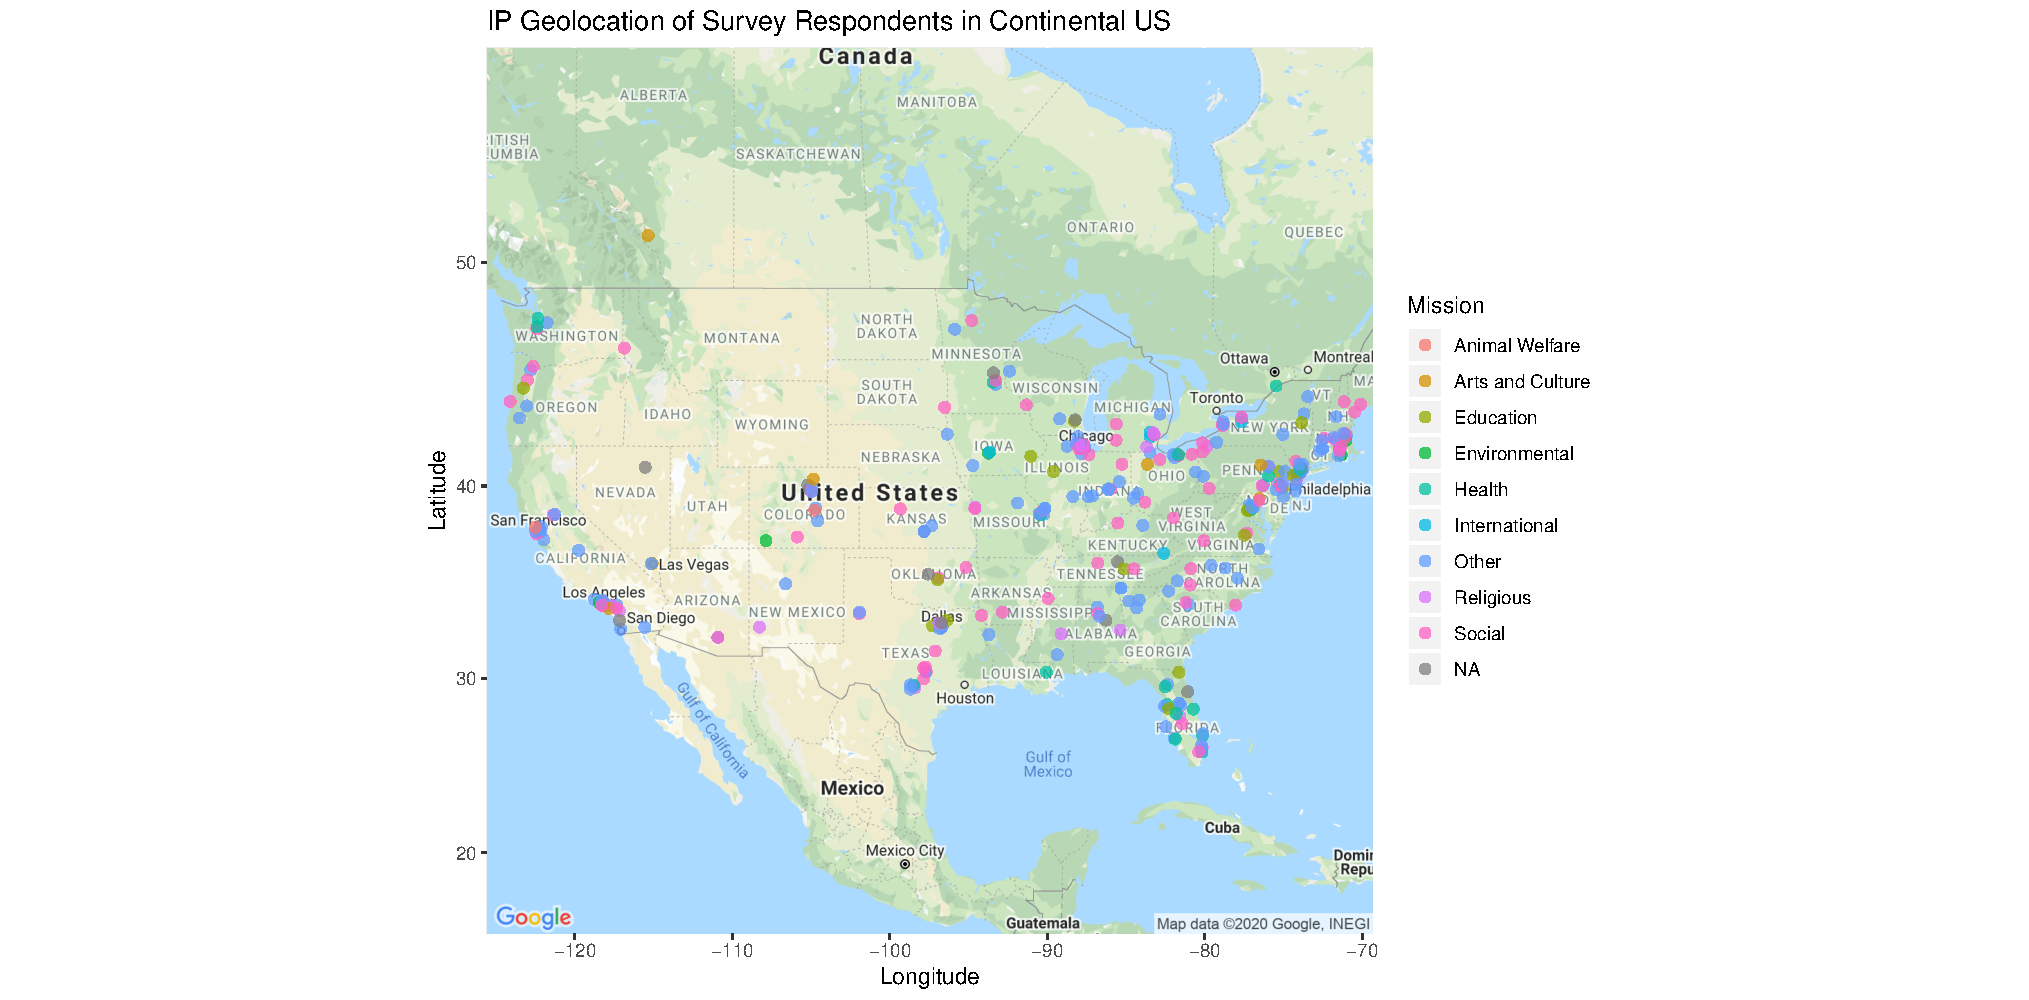
\includegraphics[width=.9\columnwidth]{surveymap.pdf}
\centering
\caption{Geolocation of Respondent IP Addresses}
\label{fig:surveymap}
\end{figure}

Table~\ref{tab:missions} summaries the general issue area provided by respondents who reported a mission area in response to the question: \say{On what mission does your organization spend the most time and money?}\footnote{137 of the respondents answered the question by describing their daily activities. These responses included day-to-day themes such as staff and payroll, as well as big-picture strategic policies, such as outreach.} These missions covered a wide thematic range, from organizations dedicated to \say{Crisis Intervention with Domestic Violence and Sexual Assault victims} to \say{Promoting mutual understanding between the U.S. and Asia} to \say{Making theater accessible to all}, to \say{Preserving the history of Hancock County, Ohio.}
% The missions described by sample respondents included 
 \begin{table}[ht]
 \centering
 \begin{tabular}{rlrr}
   \hline
  & Area & Total & Percent \\
   \hline
 1 & Animal Welfare &   3 & 2.00 \\
   2 & Arts and Culture &  12 & 7.00 \\
   3 & Education &  18 & 10.00 \\
   4 & Environmental &   6 & 3.00 \\
   5 & Health &  22 & 12.00 \\
   6 & International &   9 & 5.00 \\
   7 & Other &   3 & 2.00 \\
   8 & Religious &  17 & 9.00 \\
   9 & Social &  92 & 51.00 \\
    \hline
 \end{tabular}
 \caption{Self-reported mission areas}
 \label{tab:missions}
 \end{table}
 
The sizes of the organizations varied widely, ranging from a self-reported staff of a handful of people to large international organizations. %% Histogram of sizes 

 \begin{table}[ht]
 \centering
 \begin{tabular}{rcc}
   \hline
  Size & Personnel &  Count \\
   \hline
 Micro & 0-2 &112 \\
   Tiny &3-5 & 55 \\
   Small & 6-10 &  43 \\
   Medium & 11-20 &  5 \\
   Large & 21-50 &33 \\
   Very large & 51-100 &  15 \\
   Huge & $\geq$ 101 & 35 \\
    \hline
 \end{tabular}
 \end{table} 
 
\section{Does the transformation theory travel?}

Thus far, this chapter has argued that militant groups and non-profit organizations have a remarkable number of structural similarities. These similarities mean that non-profit managers are likely to also face a personnel resource curse, in which the rank-and-file can pressure leaders into accommodating.

In the remainder of the chapter, I present the results of surveying over 300 self-described non-profit managers for their experiences.  The questions address the points along the process, from admitting personnel who are not in alignment with the mission of the organization, to recruiting more quickly than the organization can accept, and finally to whether the managers experienced rank-and-file members contributing to a changing mission. Although the differences between legal operations and clandestine militant activity would be expected to provide more operating flexibility for leaders of the licit organizations, many of the surveyed leaders report experiencing many of the components of the personnel resource curse as well as upwards-driving pressure for change.

\section{General Views of Leader Accommodation}

To establish how the respondents view leadership, the survey asked a series of questions about respondents' beliefs about the desirability of having leaders of an organization accommodate the preferences of the rank-and-file. The majority of the survey respondents shared the expected view that recruits should be assimilated rather than accommodated. When asked in general about their views on accommodation the interests of new staff, respondents were largely not favorable to the idea of adjusting goals and mission to reflect the preferences of new members. 

The general unwillingness to change the mission of their organization to accommodate the preferences of staff and members also extended to a general aversion to the idea of changing the mission of a hypothetical organization in order to grow.  A slight majority (195) of respondents disagreed with the statement that \say{In order to attract new talent, organizations should be willing to change their goals.}\footnote{16 respondents reported that they \say{agree} with the statement, while 112 \say{Somewhat agree[d].} The respondents who disagreed were less tepid, with 72 reporting that they \say{Disagree} that organizations should change their goals to attract new talent and 123 reporting that they \say{somewhat disagree} with the statement.} Many respondents prescribed top-down management. For example, one noted \say{The changes need to start from the top down, that is how you change the culture of an organization.} Another described effective socialization and post-recruitment selection, saying that \say{the new [staff] that attempted to redirect the mission did not last more than a few weeks. It is important for a non-profit to stick to their mission if they believe in their mission.}

\subsection{Recruitment Outside of Socializing Bandwidth}

The origin of the personnel recruitment curse is recruitment outside of socializing bandwidth. As well, this is the facet of the theory that is puzzling when done by a rational leader. Thus, experiences recruiting outside of their socializing bandwidth is an initial starting point to compare the portability of the transformation theory. Moreover, if the respondents report this behavior, the cross-domain pervasiveness of this recruitment pattern contributes to the puzzle of why a rational leader would violate recruitment best practices. 

The rapid growth of staff is of particular interest because organizations have discretion and agency over their hiring, selection, and intake. This contrasts with the portrayal of many militant and social movements as seeking constant expansion, even at the expense of careful selection, socialization, or internal social endowments or recipients of new members who occasionally \say{flood} the group.\footnote{The former often underlies discussion of the political economy of so-called opportunistic rebel groups or those that expand by kidnapping new members~(\textit{e.g}~\cite{beber2013logic, blattman2010nature, cohen2013female, weinstein2005resources}). The latter framing more common in histories of movements with a nationalist or secessionist motivation. The underlying assumption seems to be that these groups also prioritize expansion, and have not implemented intricate selection and recruitment pipelines. Many of the organizations described in Chapter {[cases]} are of this type.}

The survey posed a series of questions intended to ask whether respondents had experienced personnel growth of staff, members, or the board, that could have challenged the absorption capacity of the organization. Although the bottom-up transformation theory specifically focuses on an expansion that exceeds socializing capacity, the survey concentrated instead on asking about periods of rapid growth, accommodation of the preferences of personnel or members, and short-term decisions that might undermine long-term cohesion.\footnote{The lines of questioning do not directly address recruitment beyond socializing capacity. Questions on this theme elicited a strongly negative reaction during pretesting. Framing questions as socialization failure or internal negotiation were interpreted by respondents as soliciting an admission of leadership failure.}

The results presented below focus on whether the respondent had \say{...ever been part of an organization experiencing a period of rapid growth or personnel change among the staff or the board of directors?} This question revealed a striking frequency of reports of rapid personnel change among staff, with 129 respondents reporting that they had experienced such a period.\footnote{54 respondents denied experiencing such a rapid expansion, with the remainder either giving conflicting responses or failing to answer the question.}

The results are notable for the degree to which rapid expansion of staff was more often reported than rapid recruitment of leaders: only 31 of the respondents reported having experienced quick growth of their Board of Directors and 147 specifically denied having experienced this.\footnote{63 respondents reported having experienced rapid growth on both the board and among the staff. The results are not disambiguated by organization size or general mission area, because the question asked whether the respondent had ever experienced rapid growth among staff, not whether they experienced this in their current organization.}

Of those who reported a rapid staff increase, 37 also responded that they felt that the organization's leadership should have accommodated the preferences of the new base. While only about 10\% of the total respondents, the response nevertheless indicates a sense among practitioners that bottom-up transformation may be beneficial for some organizations. Furthermore, of the 129 respondents who reported experiencing a substantial staff growth, 70 responded that they believed that the result was mission drift in their organizations. 

\subsection{Recruitment of non-aligned personnel}

A second important point of comparison is whether the non-profit leaders reported having recruited personnel who do not share the organizations' mission.

When prompted about recruitment to address specific operational needs, more respondents acknowledged (175) than denied (143) that their organizations had \say{ever needed to recruit people with essential skills or resources, even though their goals were not entirely consistent with those of the organization.} Of those who affirmed that they had needed to recruit for skills or resources rather than mission alignment, 73 responded affirmatively that \say{These personnel changes lead our mission to drift away from the priorities of the leadership.}

Figures~\ref{fig:nonalignedsize} and ~\ref{fig:nonalignedmission} presents the proportion of respondents claiming that their current organization had sought personnel for skills or resources rather than alignment. For ease of interpretation and comparison, the figures present responses clustered according to reported organization size (Figure~\ref{fig:nonalignedsize}) and reported mission (Figure~\ref{fig:nonalignedmission}). Interestingly, the theory laid out in the previous chapters frames the incentive for recruitment as likely originating from weakness and organizational fragility. The weakness pathway suggests that we would expect to see more reports of recruiting personnel with a different mission in smaller organizations. However, for those organizations with a claimed size of under 100 people, the experiences with hiring for skills rather than alignment actually increased as the organizations became larger.
 
\begin{figure}[t]
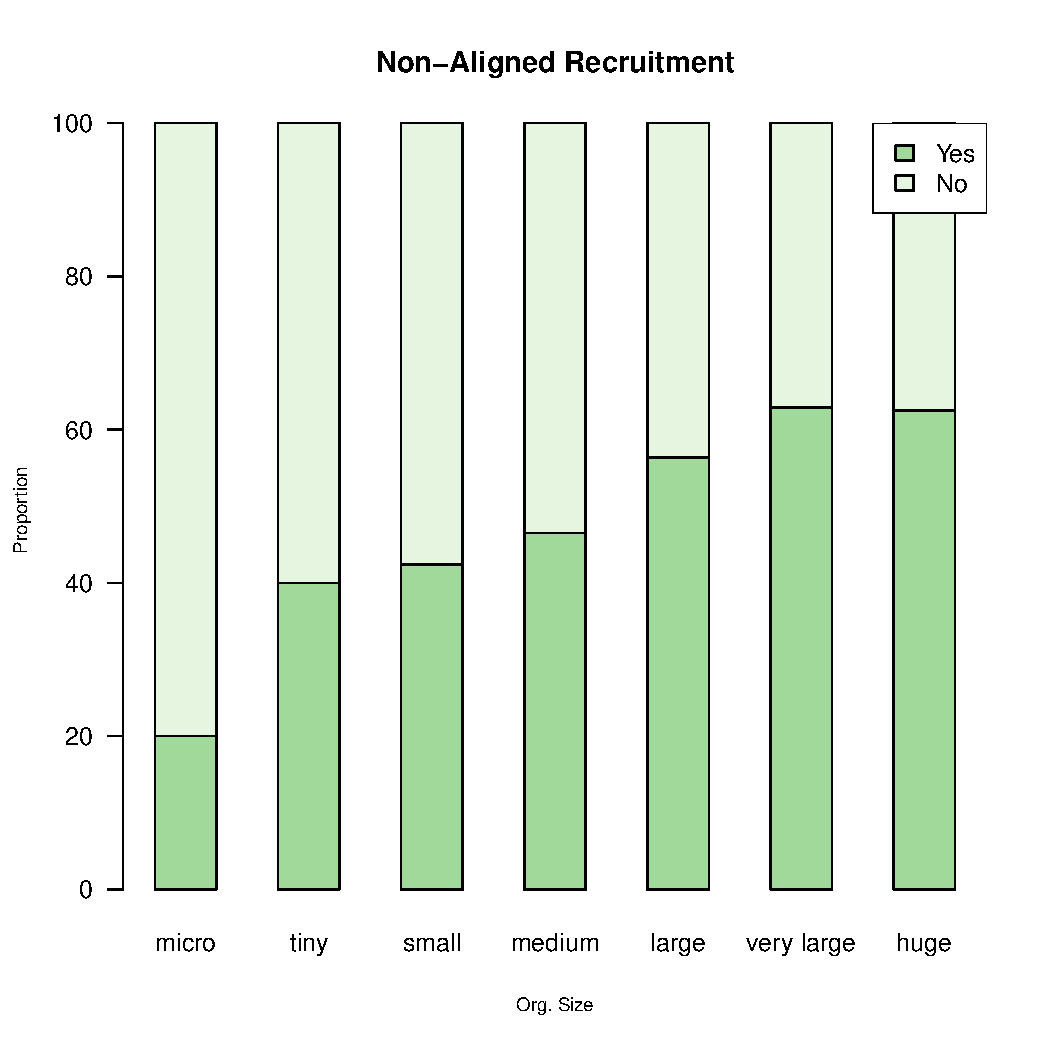
\includegraphics[width=.85\columnwidth]{./Pictures/NonAlignedRecruitmentBySize.pdf}
\centering
\caption{Reports of Recruiting Non-Aligned Staff, by Organization Size}
\label{fig:nonalignedsize}
\end{figure}

The experience with this type of recruitment pattern also changes by the self-reported mission of the respondents. Interestingly, respondents reporting that their organization is primarily involved in health-related issues were most likely to report bringing in non-aligned personnel.\footnote{16 of the 22 respondents claiming a mission that relates to health issues broadly reported this recruiting pattern.} The only individual sector larger than \say{Health} among respondents were the 92 respondents who described a mission that I clustered into the \say{Social} category. Although reporting non-aligned recruitment at a lower rate than those working on health-related issues, more than half (54 out of 92) affirmed that the organization they are part of had followed this recruitment pattern. Conversely, less than half of respondents describing a mission in the \say{Environmental,} \say{International,} and \say{Religious} clusters reported the non-aligned recruitment pattern. 

Although the survey did not ask for insight into the reasons for this recruitment, the over-representation of non-profits working in the technical and highly-licensed health domain may lend support to a pathway for bottom-up transformation that is particularly fast when personnel have hard-to-replicate skills.

\begin{figure}[t]
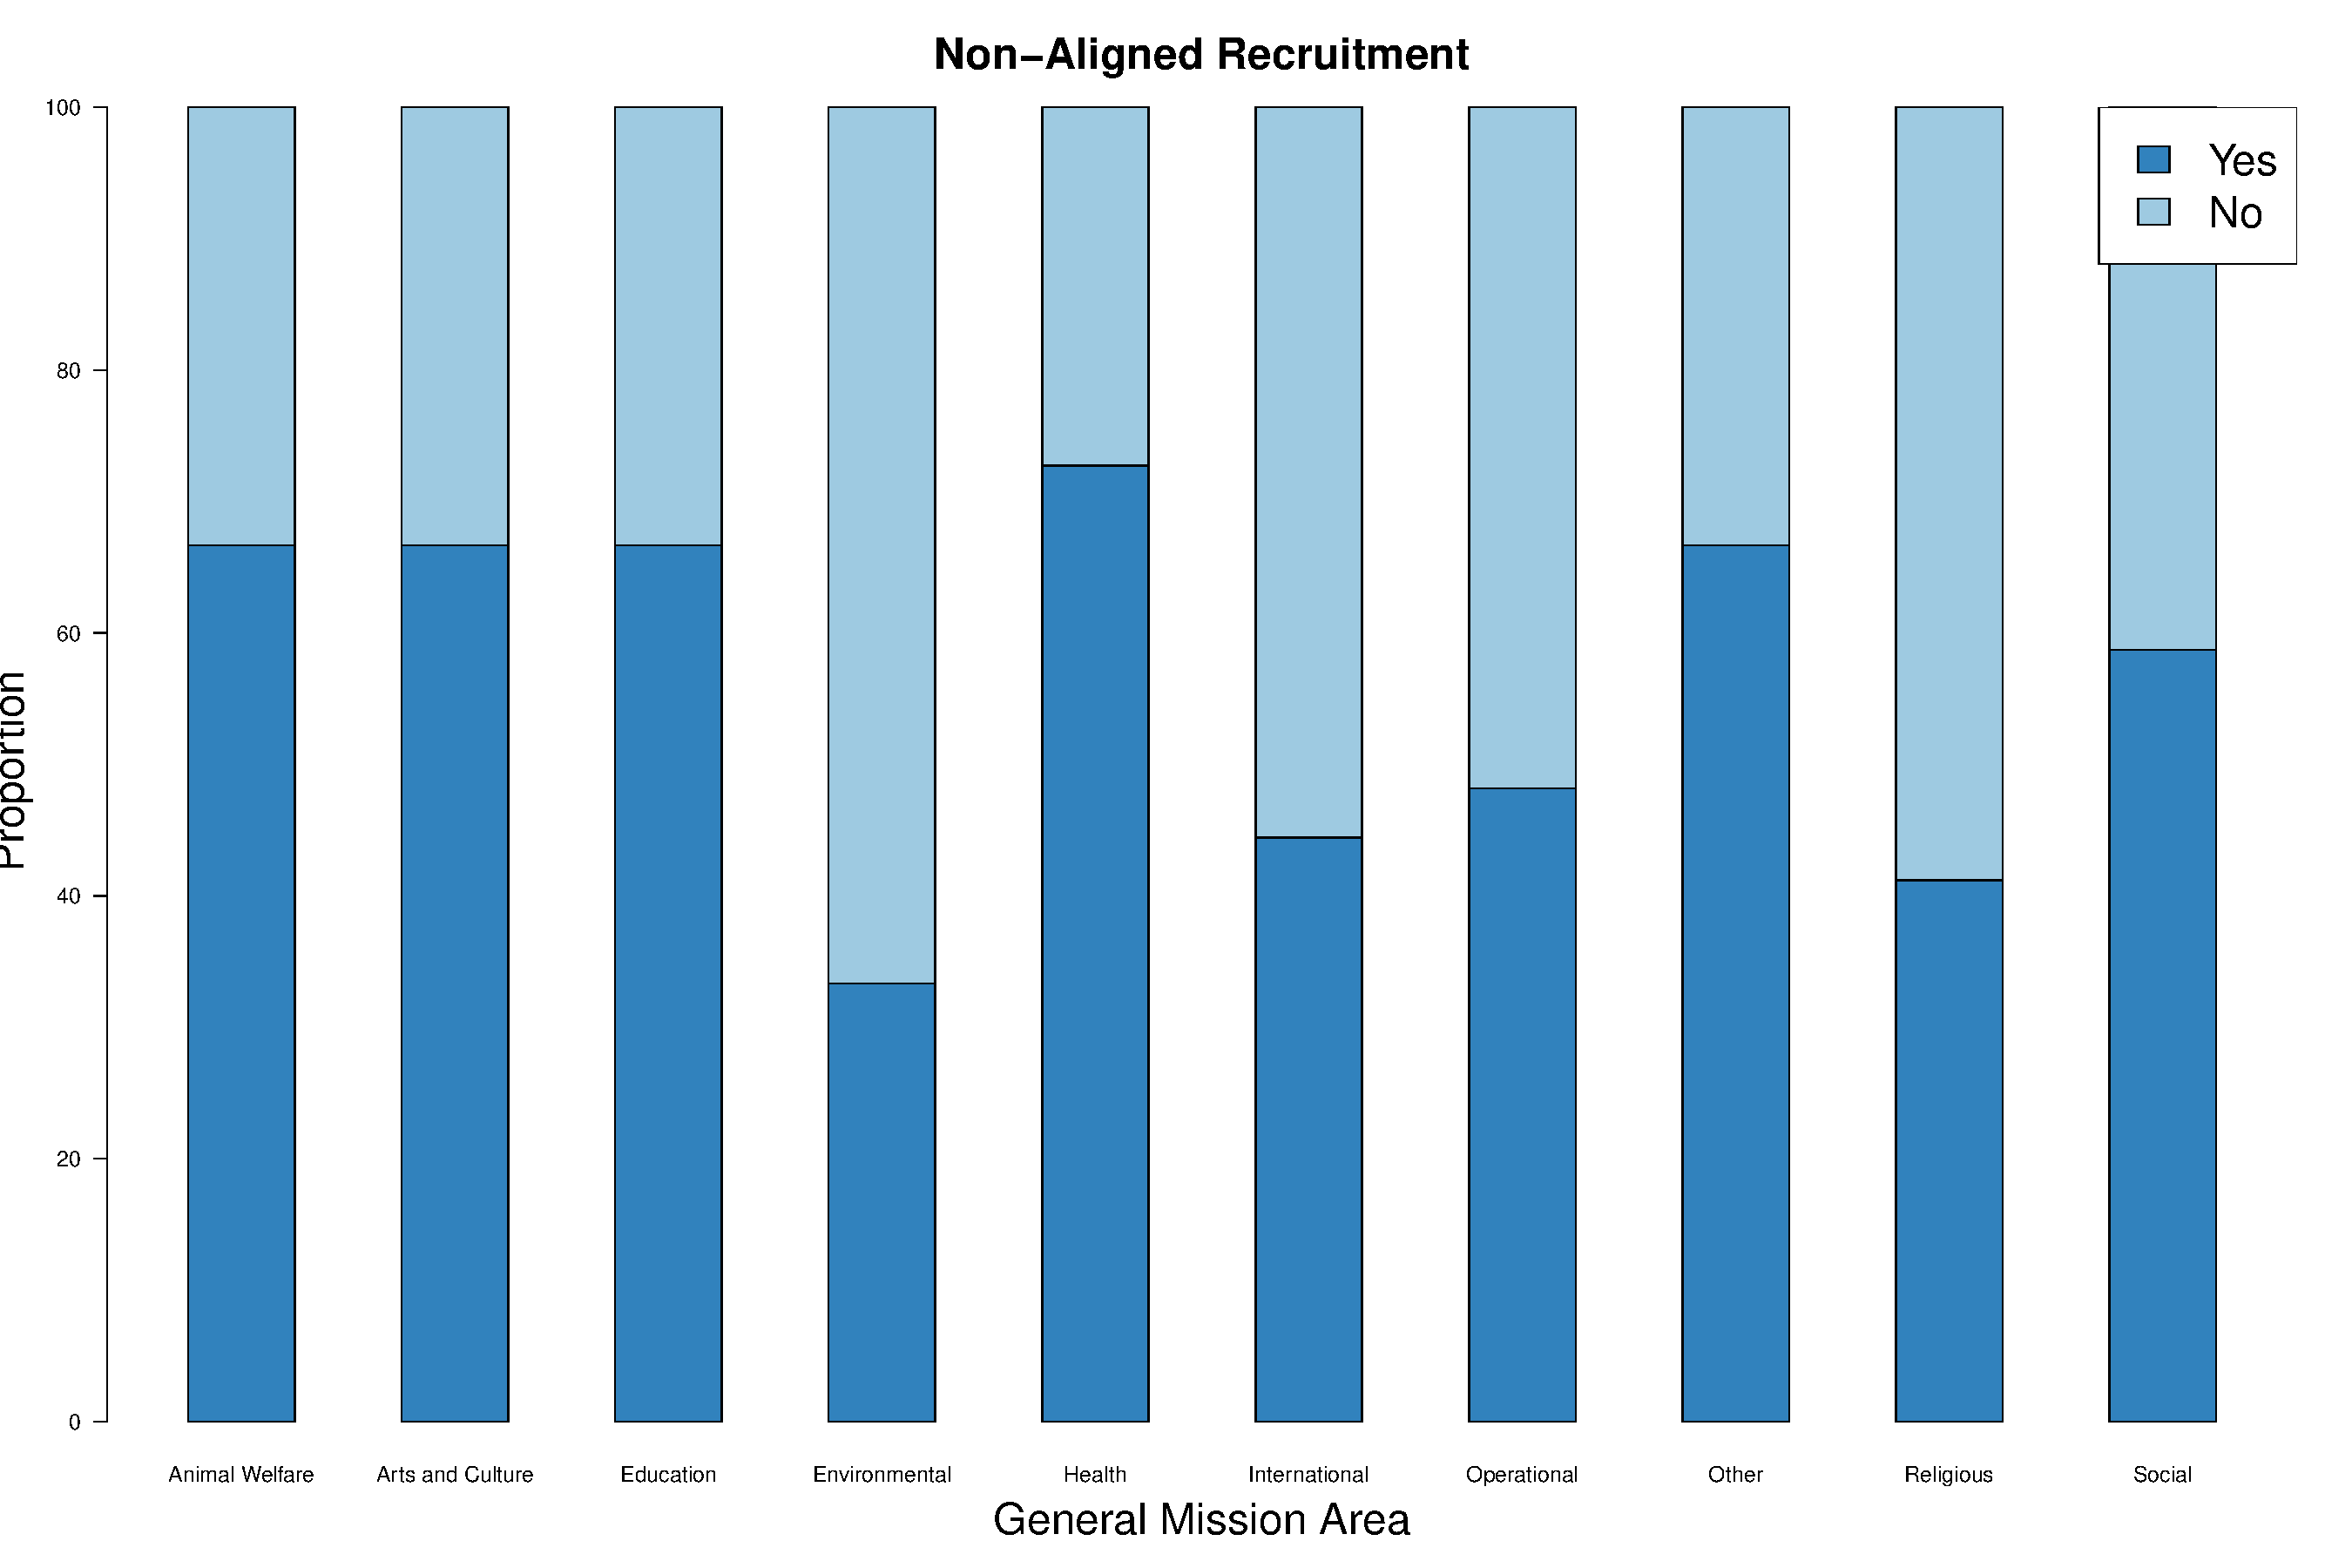
\includegraphics[width=.99\columnwidth]{./Pictures/NonAlignedRecruitmentByMission.pdf}
\centering
\caption{Reports of Recruiting Non-Aligned Staff, by Organization Mission}
\label{fig:nonalignedmission}
\end{figure}

Of those respondents who answered that their organizations had recruited personnel for reasons other than mission alignment, the survey asked whether they believed that the new personnel lead to mission drift in the organization. Of the 156 responses, 68, or 44\%, reported that they either \say{agree[d]} or \say{somewhat agree[d]} that the recruitment of non-aligned personnel resulted in mission drift. 
\subsection{Accommodation Outcome}

Among the survey takers who agreed that they had sought personnel for skills or resources rather than mission alignment, those respondents who reported that their organizations had 6-10 staff members were more likely to report subsequent mission drift caused by the personnel.\footnote{Respondents who said that they had recruited personnel for skills or resources rather than alignment were subsequently asked \say{How strongly, if at all, do you agree or disagree with the statement: \say{These personnel changes lead our mission to drift away from the priorities of the leadership?}}} The rates at which respondents reported mission drift after recruiting staff for skills or resources rather than mission alignment can be seen in Figure~\ref{fig:nonalignedMDsize}, which presents results classified according to the self-reported organizational size.

\begin{figure}[t]
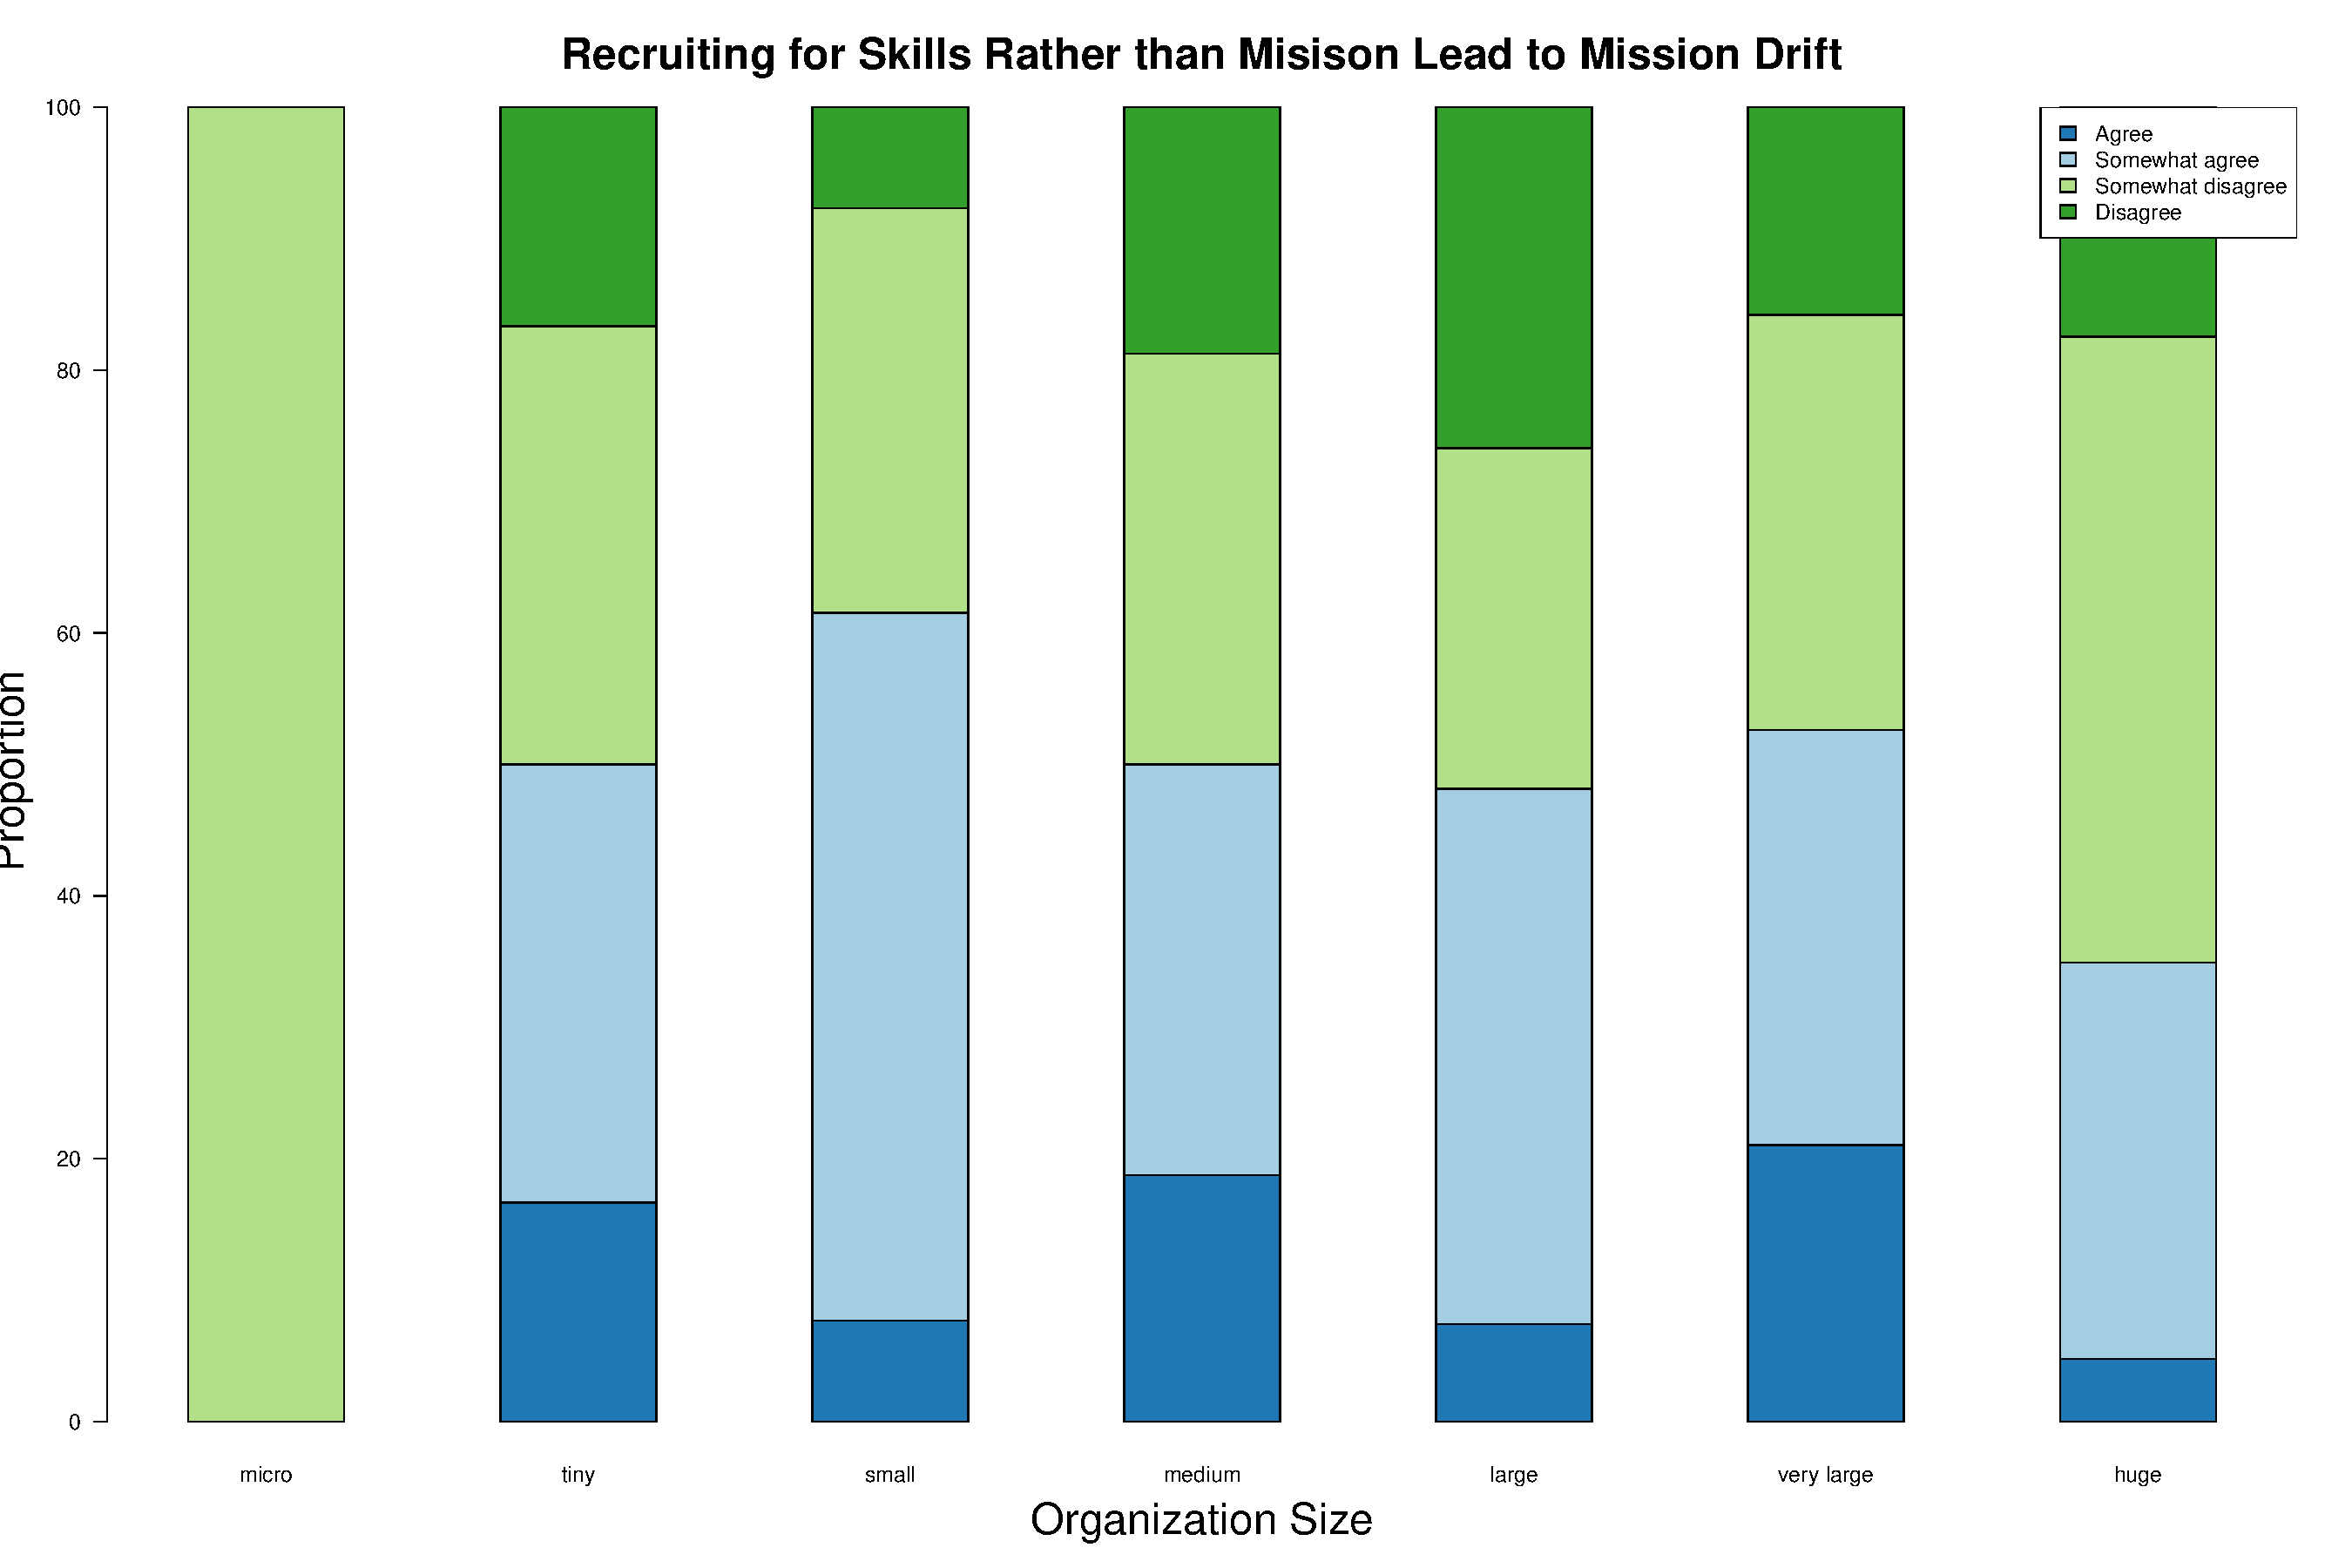
\includegraphics[width=.85\columnwidth]{./Pictures/NonAlignedRecruitmentMDSize.pdf}
\centering
\caption{Mission Drift After Recruitment, by Organization Size}
\label{fig:nonalignedMDsize}
\end{figure}

Although the \say{health} cluster reported the most recruitment of non-mission aligned personnel, they reported this personnel-driven mission drift at lower rates than Arts and Culture or Educational organizations. Figure~\ref{fig:nonalignedMD} presents the percentages of respondents in each cluster of missions who, after agreeing that their organizations had recruited for skills or resources rather than buy-in on mission, did or did not agree that mission drift was a downstream result of this recruitment. 

\begin{figure}[t]
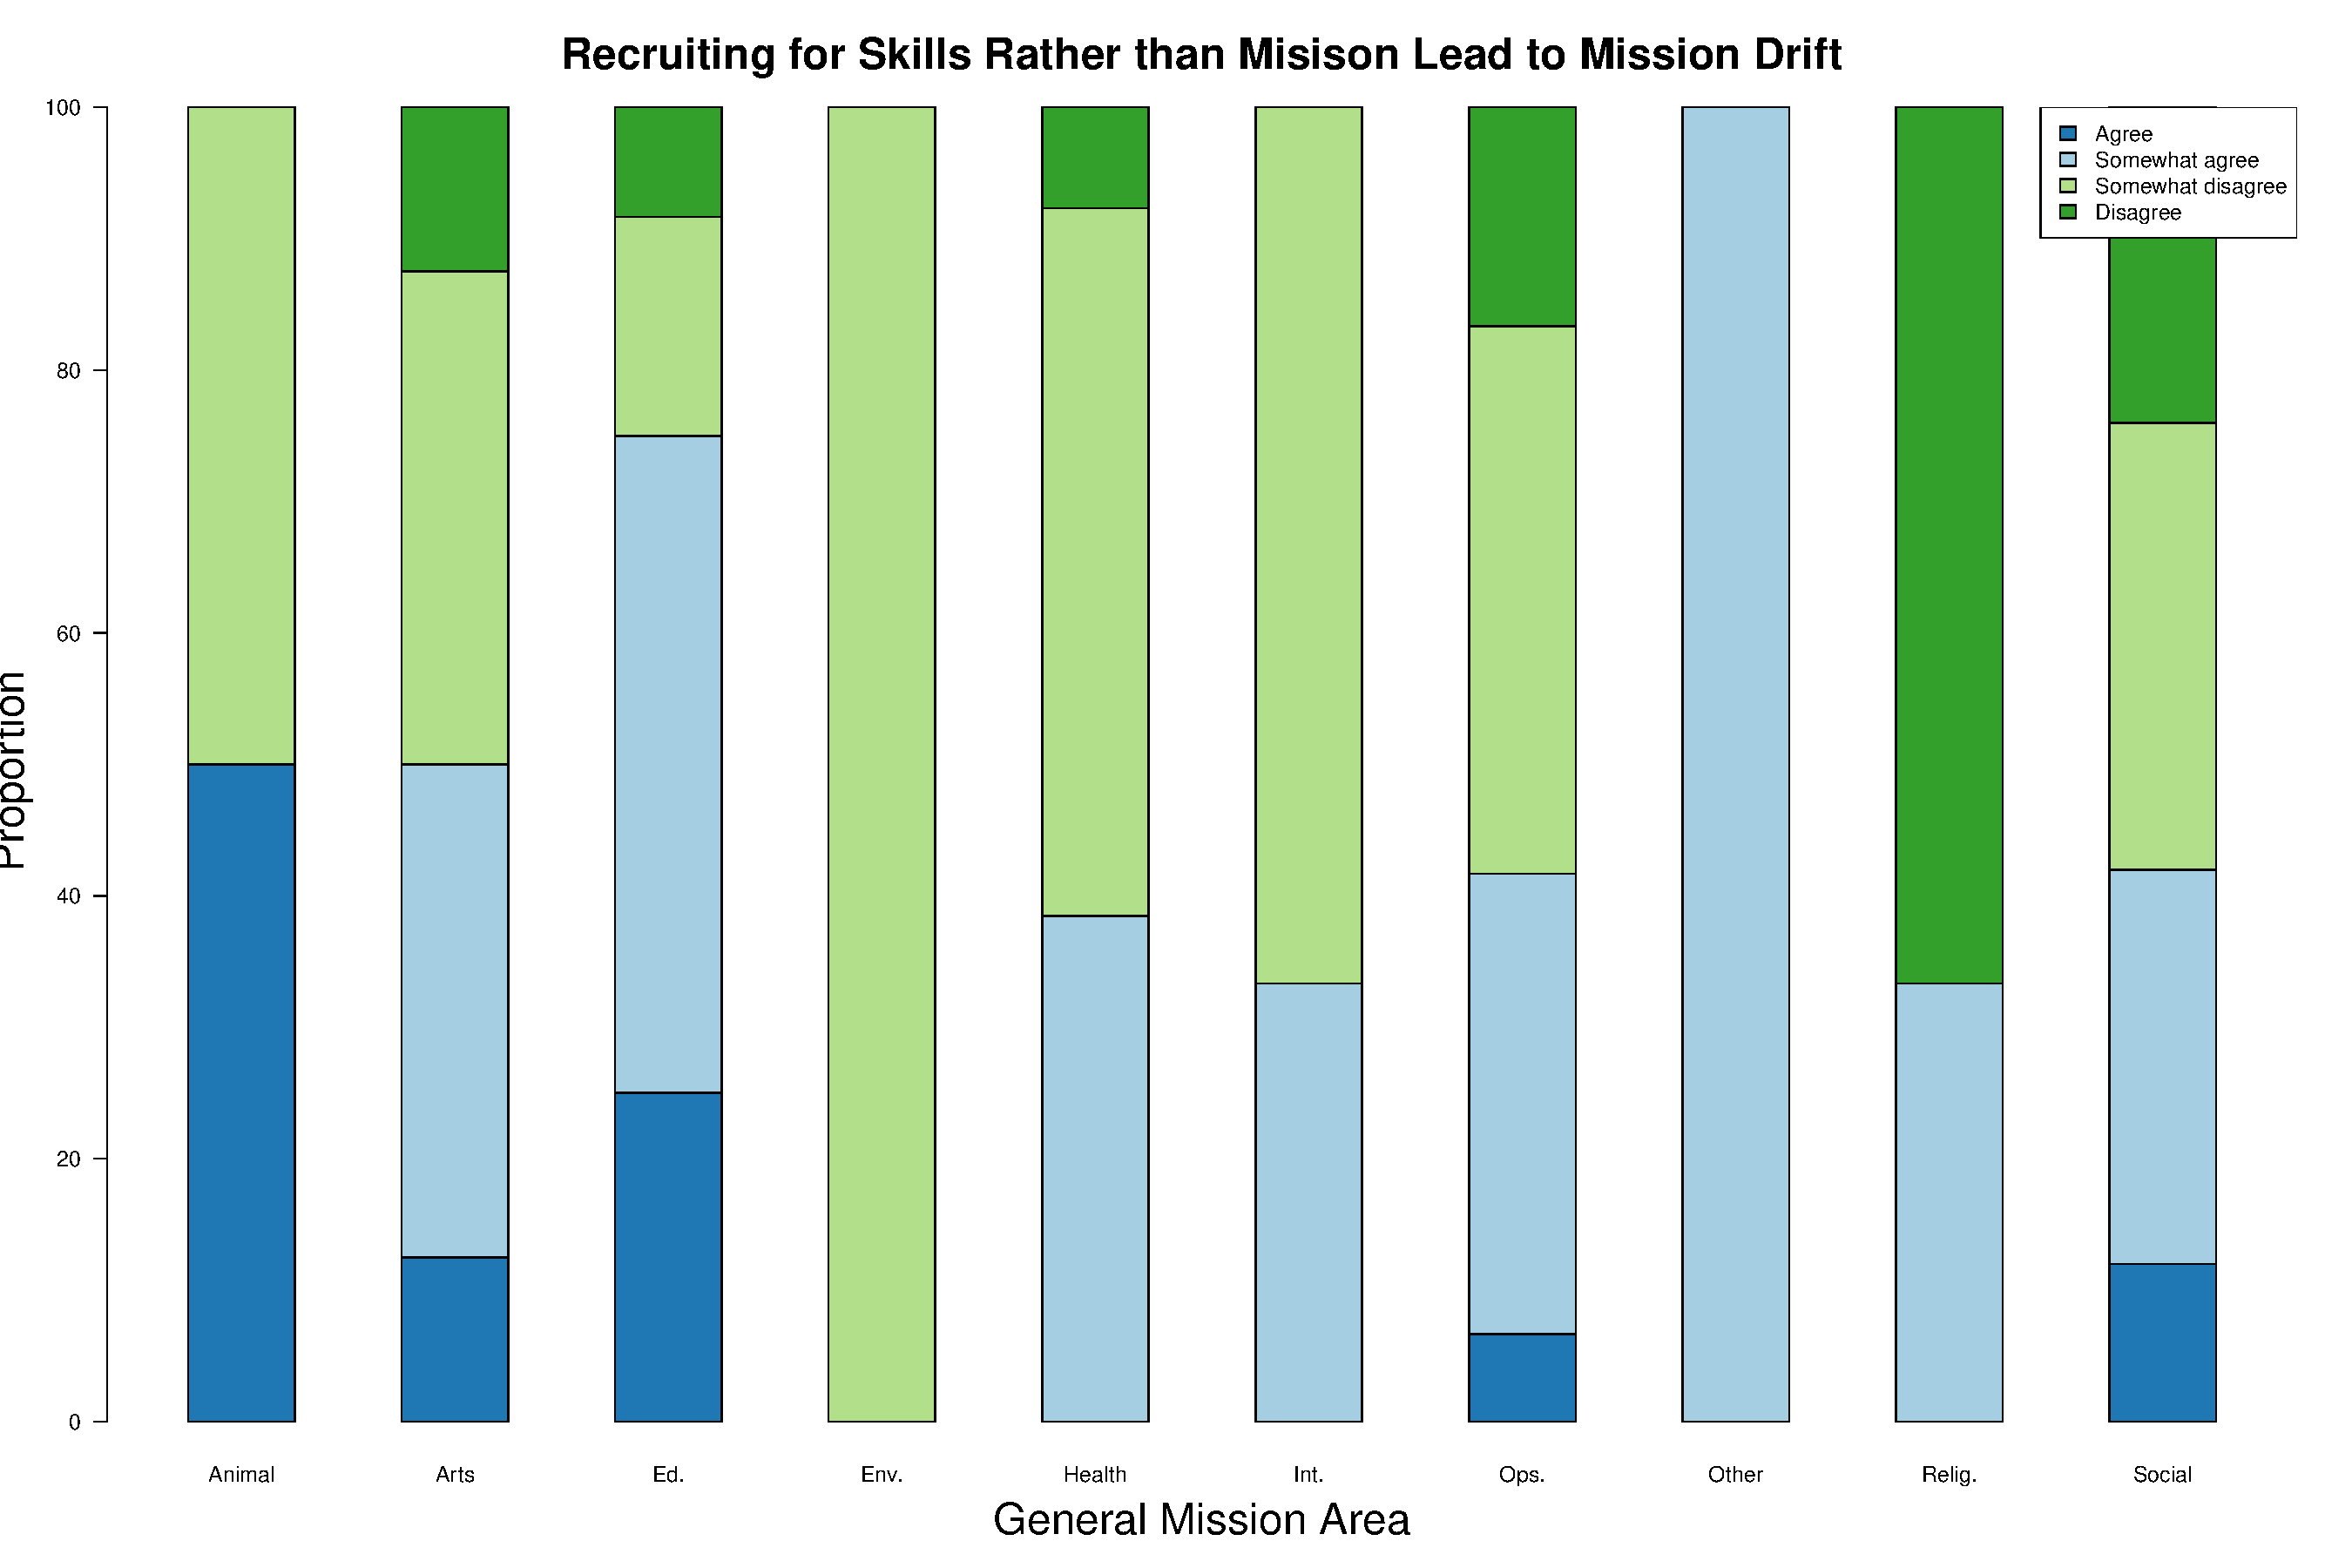
\includegraphics[width=.95\columnwidth]{./Pictures/NonAlignedRecruitmentMD.pdf}
\centering
\caption{Mission Drift After Recruitment, by Type of Mission}
\label{fig:nonalignedMD}
\end{figure}

Survey respondents described their experiences with organizations accommodating new staff. One respondent, located in Miami, noted that in their experience recruiting for skills rather than alignment, the consequence was that \say{changes originated in the changes that were demanded by the members.  The org had to respond or risk losing members.} Another, writing from Southern Maine who identified their organization as a provider of \say{social service [sic],} concluded that the recruitment resulted their group having \say{lost some of our identity} because \say{Changes originated from new staff members who came with their own agenda.} A third--- geolocated to Des Moins, Iowa and reporting that their organization was involved primarily in \say{worldwide missions}--- added: \say{When the staff does not fully embrace and agree with the mission of the organization, then things begin to happen (events, discussions, etc) that begin to steer the organization away from its mission.}

\subsection{Factorial Experiment}

The second half of the survey was designed to test the expectation that leaders can be induced to admit recruits with heterogeneous preferences.  The experiment was administered alongside the non-profit leader survey, and resulted in 291 responses.

The experiment asked respondents to assess two potential candidates for each of a position on the Board of Directors for their organization and a staff role. The conditions included variation on the degree of alignment with the organization. For the potential staff members, the potential personnel also varied in the percentage to which their salary and benefits would be subsidized. These subsidies were either 0, 25\%, 50\%, or 75\%. Potential staff members were characterized as having a preferred mission that was \say{a little different than,} \say{very different than,} and \say{very similar to} the existing mission of the organization. Despite the theory's focus on grassroots organizational members, the experiment included a vignette for potential Board members as well as staff to provide a basis of comparison in how the participants view potential leaders. 

As salaries and benefits are not salient for members of a Board of Directors, prospective Board members varied on whether they would \say{bring needed professional skills} to the Board. Both vignettes noted that \say{You expect that if they join, they will try to steer the organization's mission to align with their goals.} This phrase was included to underscore the expectation that a forward-looking leader would recruit new personnel even knowing that the new staff will attempt to change the direction of the organization, 

The factorial design instructed the respondents to consider that the organization that they were hiring for had a resource level that was ~\say{secure and stable},~\say{barely sufficient}, or~\say{precarious— not sure if operations will continue}. This feature connected the prompt from the factorial to the expectation that survival pressures would induce leaders to accept potential staff or board member with preferences further from their existing mission.

The vignettes thus presented a menu of potential staff or Board members, an accompanying resource or skill inducement, and an underlying condition of scarcity. Without influence of the resource or skill inducements, respondents should gravitate towards those candidates whose preferences are \say{very similar to} those of their organizations. If external subsidies can induce leaders to admit recruits with heterogeneous preferences, selection of staff or potential board members with different preferences should increase in the promised skills or salary subsidy. 

The degree to which each condition contributed to respondent preferences can be seen in Figure~\ref{fig:factorial}, plotted via the Cregg package for R~\autocite{leeper2018cregg}. The Marginal Mean plot depicts the impact of each condition on the likelihood of respondents choosing a candidate with each trait. Values above 0.5 indicate features that increase the profile's likelihood to be selected, while those below 0.5 decrease the profile's propensity to be selected.  In assessing individual features, the survey respondents were consistently most likely to select a candidate described as having a mission preference very close to the organization. Although the experiment results do not reflect the expectation of the formal model, the results underscore the degree to which rapid recruitment of members with heterogeneous preferences occurs despite, rather than because of, leader preferences.

%% Looking for any combinations in the factorial that show that they do have
%% some kind of trade-off (is there any pair of things that are interesting and suggestively  supportive)

\begin{figure}[t]
\centering
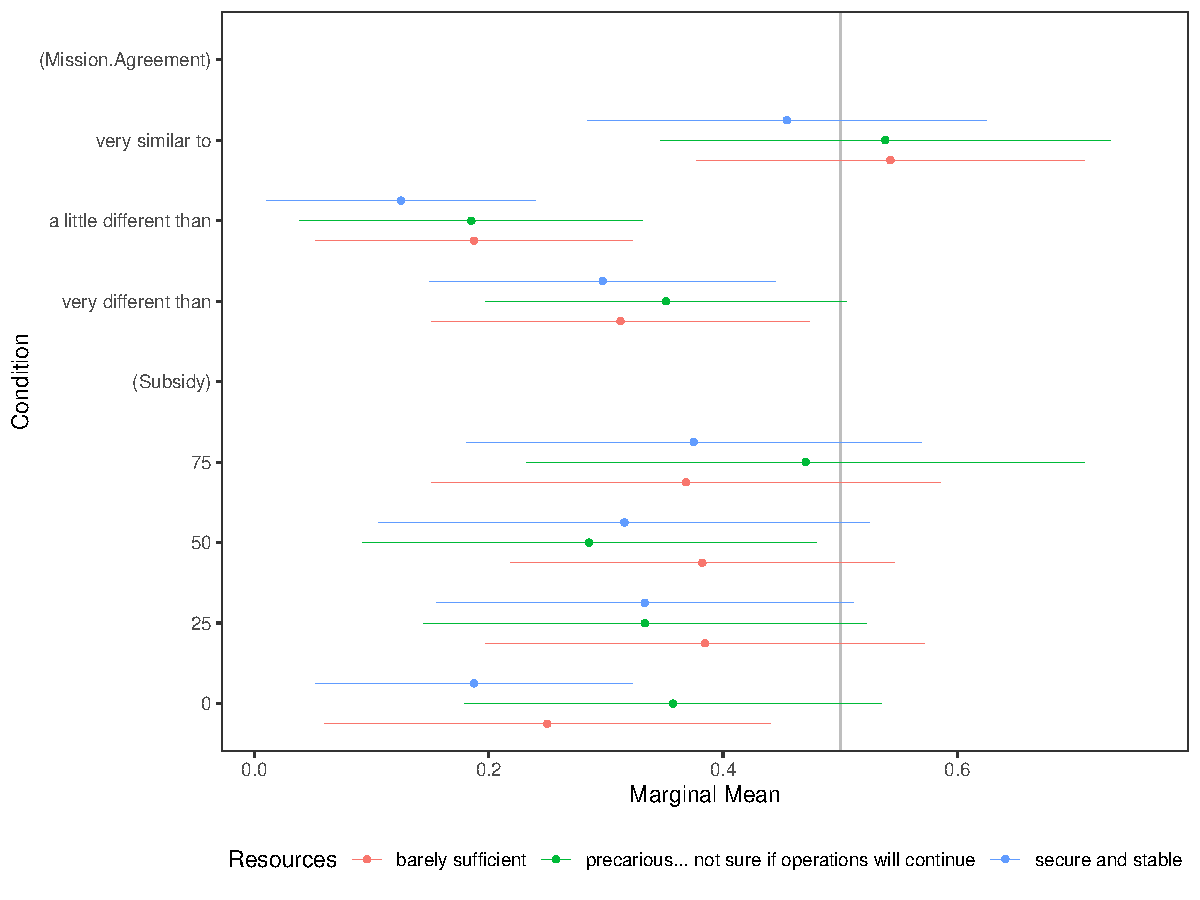
\includegraphics[width=.85\columnwidth]{./Pictures/simpleConjoint.pdf}
\caption{Baseline Results of Factorial Experiment}
\label{fig:factorial1}
\end{figure}


%% Summarize that in the morning of 2/24


\section{Conclusion}

This chapter has sought to demonstrate that the core insights that drive the Personnel Resource Curse apply in domains other than the militant groups that have formed the focus of previous chapters of the dissertation. It has had twofold goals. First, to demonstrate that the apparently-puzzling behavior of organizational leaders accepting large numbers of new personnel whom they will be unable to socialize into the existing mission is not a pathology specific to the operational demands of militant groups. 

The first goal is important to expand the theory outside of the domain of militant groups. Finding cross-domain applications of the theory has important implications. First, finding similar behavioral patterns in a separate domain is reassuring for the framing of the Personnel Resource Curse as a general theory of organizational change. 

Second, it provides an independent domain in which to test the predictions of the theory, and thereby provides an opportunity to avoid circular reasoning of using the same cases and domain both for theory development and testing. This builds on the work of scholars who have argued that militant groups are not completely \textit{sui generis} and can thus be analyzed and countered using conceptual tools developed in other domains.

The chapter presented the results of asking non-profit leaders and managers whether they had ever experienced a rapid intake of personnel that do not share the organization's original mission in order to demonstrate that the initial recruitment shock that initiates the process is not unique to militant or clandestine groups. The finding that a substantial minority of the respondents had experienced this type of growth provides a strong signal that this organizational pattern is not an idiosyncrasy of militant groups. As well, it gives an initial estimate of the frequency at which organizations may experience recruitment shocks that result in downstream consequences. 

It provides support for the specific theory of upward-driving organizational change by establishing that among the sample of non-profit leaders surveyed, there is a non-trivial baseline belief that they have experienced mission-drift after recruitment. Experiences with bottom-up mission drift were reported alongside claims that change should originate with leaders and that new recruits should conform to their new organizations. This parallel's the theory's expectations that bottom-up transformation should occur despite, not because of, leader preferences.

Finally, the chapter presented a factorial experiment designed to test the prediction from the formal model that leaders can be induced by circumstances to recruit non-aligned members even knowing that they will eventually have to accommodate their preferences. The experiment focused on whether the combination of organizational precarity and external subsidies could induce leaders to knowingly hire either staff or board members that would try to change the organization. The results did not support the expectation that those leaders who were presented with a situation of resource scarcity would be more willing to hire new staff who did not align with their mission. This finding may be consistent with the observation that the rapid recruitment is a feature of many organizational histories, despite being against recruitment best practices.  When presented with an abstract condition, the leaders were uninterested in recruiting new personnel who would attempt to redirect the group, even with the dual inducements of financial stress and a deep discount on the prospective member. 




}
\include{{./Chapter1-Introduction/Conclusion}}
%==============================================================================

%-----------------------------------------------------------------------------%
% APPENDICES -- OPTIONAL. These are just chapters enumerated by Appendix A,
%                Appendix B, Appendix C...
%-----------------------------------------------------------------------------%
\appendix
\chapter{Formal Model}
\label{modelappendix}

The game has two rounds of play, each with four stages.\footnote{The two rounds of action generates complex notation. In the appendix, the first super/subscript number indicates the round in which the action occurred and the second indicates the case. So, $\act{1,2}$ represents the second case of the first round action proposal.} The actions formalize the theory's intuition that operational decisions require the assent of both the organization's leaders, who set and guide a strategic vision, and the rank-and-file who will ultimately carry out the actions. The need for internal agreement gives rise to an internal bargaining process in which leaders will explicitly or implicitly adjust to the actions that their followers will support.

The game that follows formalizes this process and extends the decision tree backwards to the point at which a Leader chooses whether or not to recruit, knowing that the new members will eventually wield influence.

Thus, each round proceeds as follows:

\begin{enumerate}
\item Leader recruits or not
\item Recruit accepts membership offer or not
\item Leader proposes a new activity
\item Recruit accepts or rejects the activity
\item The activity succeeds or fails, with a probability proportional to the level of resources that the Recruit brings to the organization.
\end{enumerate}

Figure~\ref{fig:extform} depicts one round of the game in extensive form.
\begin{figure}
  \centering
  \includegraphics[width=.85\columnwidth]{../Pictures/RecruitGame_Round1.pdf}
  \caption{Recruitment Game, Extensive Form}
  \label{fig:extform}
\end{figure}

The solution concept is backwards induction. This is appropriate because the game is one of complete information and two rounds of play. Although simple, designing the game as one of complete information highlights the degree to which a Leader may
embark in an organization-transforming recruitment process
\textit{even knowing} that in equilibrium they will be obliged to updated their own eventual goal to include the preferences of the Recruit. 

To summarize the conditions of the equilibrium: the Recruit accepts ($a$) the proposed activity when their expected utility of a successful outcome ($s$) is at least as large as the expected utility of rejecting ($r$) the activity. The probability of success ($\ps{}$) is proportional to the level of resources ($R_{R}$) that the Recruit brings to the organization. The expected value of the recruit's socialization goals is $\egoal{1}$

\section*{Notation}

The equilibrium outlined below uses the following notation:
\begin{itemize}
\item Proposed actions are denoted with \textit{a}
\item Goals are denoted with a \textit{G}, with $G^{n}_{L}$ indicating
  the \textit{Leader's} goal for the $n^{th}$ update and $G^{n}_{R}$ indicating the \textit{Recruit's} goals for the $n^{th}$ updating.
  \item Costs are denoted with \textit{C}
  \begin{itemize}
  \item $C_{a}$ are the costs associated with the action.
  \item $C_{I}$ represents the Leader's costs to gather information about the potential Recruit.
  \item $C_{S}$ is the Leader's costs to socialize the new Recruit.
  \end{itemize}
    \item $\delta$ is the Leader's capacity to socialize the
      Recruit. It is function of the Leader's strength ($S_{L}$) and the Recruit's resistant capacity($S_{R})$.
      \item After the first round action, the Leader's goals update to represent a linear combination of the Leader's original goal and the previous round's action, weighted by $\alpha$. This updated goal is $\lgoal{1} = \alpha\lgoal{0}+(1-\alpha)\act{1}$
\end{itemize}

As the solution concept is backwards induction, analysis of the
conditions for equilibrium begin from the terminal node and work
backwards through the game.

\section{Second Round}

\textbf{Summary of equilibrium:}

%The leader recruits when $\lgoal{1}= \alpha \lgoal{0}+(1-\alpha)\act{1}$.
% By definition true, so not the equilibrium.

%has to be + between the two terms, or the updating doesn't work....
The Recruit accepts the offer if their expected utility after socialization is greater than the loss of utility for not being part of a group. This cutpoint occurs when: $|\rgoal{2}-\act{2}|\leq \gamma + \frac{U_{G}- |\delta(\rgoal{1}-\lgoal{1})|}{\ps{}}$, where $\gamma = 1- \frac{C_{a}}{P_{R}}$.  In the first round, the Recruit accepts with the same utility function, as it is a different recruit, and so from their perspective, the game is only a single round. Correspondingly, the Leader offers members if the cutpoint holds and the Leader's expected utility for the section action proposal is greater than zero ($EU^{2}_{L}(a^{*}_{2}) \geq 0$).

\underline{Full characterization of second round}

The Recruit's expected utility is: $EU^{2}_{R} = \ps{}(1- |\rgoal{2}- \act{2}| - \cost{} - |\rgoal{1}-\rgoal{2}|)$. They accept the action proposal $\act{2}$ if $EU^{2}_{R} \geq |\rgoal{1} - \rgoal{2}|$ or $P(R)[1- |\rgoal{2}- \act{2}| \geq \cost{}]$

In order for the Leader to propose an action the action must be chosen such that $\ps{}[1-|\lgoal{1} - \act{2}|] \geq \cost{}$ and $\ps{}[1-|\rgoal{2}- \act{2}|] \geq \cost{}$. Given this constraint, and the Recruit's acceptance cutpoint, the Leader chooses an action proposal, \act{2}, to maximize $\ps{}[1 -|\lgoal{1}-\act{2}|- \cost{} - \infocost{} - \socialcost{}]$. 

The Leader's maximization produces two cases:\\
Case (1): $\rgoal{1} \leq \lgoal{1}$\\
Case (2): $\rgoal{1} > \lgoal{1}$\\
In Case (1) if $|\lgoal{1}- \rgoal{2}-\gammacust| \leq \gammacust$, then $|\lgoal{1} - \act{2}| \leq \gammacust$ and $|\rgoal{2}- \act{2}| \leq \gammacust$ and  $\act{2} = min(\lgoal{1}, \rgoal{2} + \gammacust)$\\
If not, $\act{2} = \lgoal{1}$

In Case (2) if $|\rgoal{2} - \lgoal{1}- \gammacust| \leq \gammacust$,  $\act{2} = max(\lgoal{1}, \rgoal{2}-\gammacust)$\\
If not, $\act{2} = \lgoal{1}$\\

Moving up the game tree, the Recruit accepts the offer of membership if their expected utility from the action proposal $\act{2}$ is at least as high as their expected utility from being in the group. At this decision, the Recruit accepts if $EU^{2}_{R} \geq U_{G}$. 
This decision takes into account the expected effects of socialization, and so the potential Recruit agrees to join the group when $\rgoal{2}= \delta(\lgoal{1}- \rgoal{1}) + \rgoal{1}$ and  $|\lgoal{1}-\rgoal{2}|= |\delta(\rgoal{1}-\lgoal{1})|$. 

Combining the point at which the Recruit agrees to join the group and their expected level of socialization, the Recruit joins when:\\ $\ps{} (1-|\rgoal{2}- \act{2})|\geq \cost{} - U_{G} + |\delta (\rgoal{1} - \lgoal{1})|$\\
This condition simplifies to: 
$|\rgoal{2}- \act{2}| \leq \gammacust + \frac{U_{G} -|\delta(\rgoal{1}-\lgoal{1})|}{\ps{}}$

The Leader offers membership if the recruit will accept, and if the $EU_{L}^{2}(\act{2}) \geq 0 $

\underline{Full characterization of first round}\\
 
 The Leader selects an action proposal such that the action will maximize  $EU^{1}_{L}= \ps{}(1-|\lgoal{0}- a^{*}|) - \infocost{} -\socialcost{}- \cost{} -|\lgoal{1} - \lgoal{0}|$

Because the Leader proposes an action, $a^{*}_{1}$, that will be accepted by the Recruit, the expected utility becomes:\\
$\ps{}(1-|\lgoal{0}- \act{1}|)- \infocost{} - \socialcost{} -\cost{}- | \lgoal{1}-\lgoal{0}| \geq - \infocost{} - \socialcost{}$.

Replacing $\lgoal{1}$ with $\alpha\lgoal{0}+ (1-\alpha)\act{1}$ allows the equation to be simplified to:\\
$\ps{}-[\ps{} + (1-\alpha)](|\lgoal{0}- \act{1}|)\geq \cost{}$\\
$|\lgoal{0}- \act{1}| \leq \frac{\ps{}- \cost{}}{[\ps{} + (1-\alpha)]}$

As the initial conditions to arrive at the first round recruiting stage are true (\textit{i.e.}: that the Leader wants to offer recruitment options that the potential Recruit will accept), this condition implies that $|\rgoal{1}- \act{1}|\leq \gammacust$ and, from the above, $|\lgoal{0}- \act{1}|\leq \frac{\ps{}- \cost{}}{[\ps{} + (1-\alpha)]}$.

This creates two situations for the Leader: (1) when $\rgoal{1}\leq \lgoal{0}$ and (2) when $\rgoal{1} > \lgoal{0}$.

In case (1), where $\rgoal{1} \leq \lgoal{0}$,  if $|\lgoal{0}- \rgoal{1} - \gammacust| \leq \frac{\ps{}- \cost{}}{[\ps{} + (1-\alpha)]}$, $\act{1} = min(\lgoal{0}, \rgoal{1} + \gammacust)$  If not, $\act{1} =\lgoal{0}$.

In case (2),  $\rgoal{1} > \lgoal{0}$. In this case $\act{1}= max(\lgoal{0}, \rgoal{1}- \gammacust)$ when $|\rgoal{1}- \lgoal{0} - \gammacust| \leq \lgammacust$. If not, $\act{1} =\lgoal{1}$. If this case is not satisfied, the recruit accepts according to the same condition as in the second round: $|\rgoal{2}- \act{1}| \leq \gammacust + \frac{U_{G} -|\delta(\rgoal{1}-\lgoal{1})|}{\ps{}}$

Finally, the Leader initiates the recruitment cycle when: the Recruit will accept and $EU_{L} \geq 0$ where the expected utility of the Leader is: $EU^{1}_{L}= \ps{}(1-|\lgoal{0}- \act{1}|) - \infocost{} -\socialcost{}- \cost{} -|\lgoal{1} - \lgoal{0}|$} 
\chapter{Supporting Information For Text Analysis}
\label{textappendix}


\section{Introduction}

This appendix presents supporting information for the quantitative analysis sections of Over Pressure: Grassroots-Driven Transformation of (Militant) Organizations. The analysis covers the data selection, processing, and results for a random forest, support vector machine, and t-Distributed Stochastic Neighbor Embedding (t-SNE) clustering of news articles about violence in Yemen attributed to AQAP, Ansar al-Shariah, and the Houthi militant groups. It also describes the data, analysis, and results for a Structural Topic Model of communications from AQAP, Ansar al-Shariah, and as-Sahab.

\section{Media Texts and Processing}

News stories originated in the ICEWS database and were selected by
first querying the database for stories about events located in Yemen. This
resulted in 47,385 stories ranging from January 15, 1991 through January 4,
2015. I selected only \say{violent} events, defined as events that
fall into one of the following ICEWS event types: \say{Threaten with
military force,} \say{Use unconventional violence,} \say{Violate ceasefire,}
\say{Use as human shield,} \say{Threaten,} \say{Occupy Territory,} \say{Physically
assault,} \say{Mobilize or increase armed forces,} \say{Engage in violent
protest for leadership change,} \say{Engage in mass killing,} \say{Conduct
suicide, car, or other non-military bombing,} \say{Carry out suicide
bombing,}\say{Attempt to assassinate,} \say{Assassinate,}\say{Abduct, hijack, or
take hostage,}\say{Fight with small arms and light weapons,} or \say{Fight with
artillery and tanks.}

This resulted in 10,818 stories, of which I took a random sample of
1772 stories. ICEWS codes for event date, event type, source actor,
and target actor. However, the source and target actor codes typically
characterize the actor by their role, such as \say{Armed Rebel} or
\say{Militant,} rather than by group affiliation.

\begin{figure}
\begin{center}
\begin{tabular}{c}
 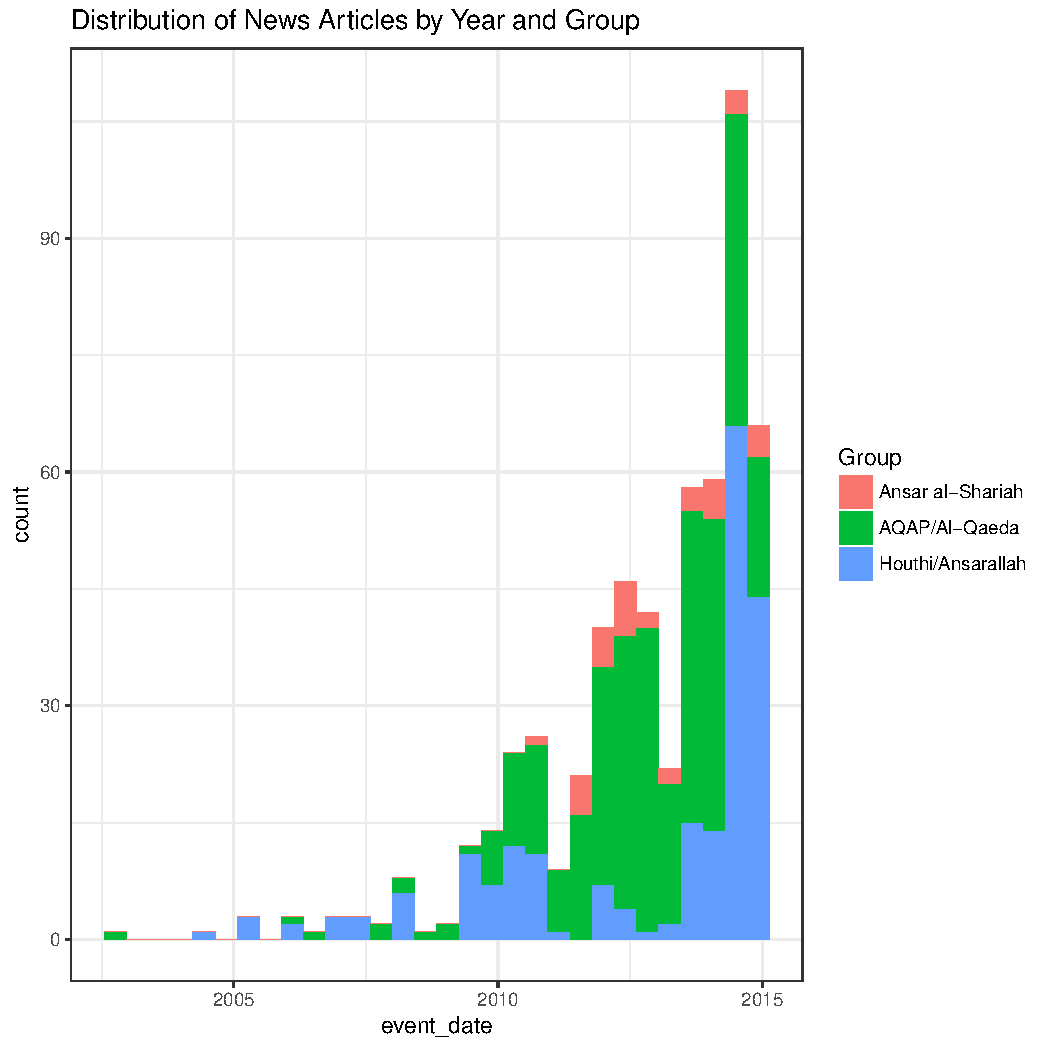
\includegraphics[width=5.00in]{./Pictures/storyHistogram.pdf}
\end{tabular}
\caption{Distribution of News Articles}
\label{fig:news-hist}
\end{center}
 \end{figure}

In order to generate data on how groups operate, I re-coded the reports to include a
variable for group or movement affiliation. I first sent the sample to
Amazon's Mechanical Turk platform, asking the workers to categorize
the stories as relating to an action carried out by Ansar al-Shariah,
AQAP, Houthi/Ansarallah, Yemeni Government, Tribal Uprising, Other,
Multiple Actors, or Unknown.  I kept the tags for the 283 stories that
both coders agreed on, and hand-coded the remaining 1489 stories. The temporal distribution of
the news articles and actor labels can be seen in Figure~\ref{fig:news-hist}. I
then further subset the data to keep only the stories tagged as
describing a violent event carried out by one of the three militias of
interest. This produced the final 720-story corpus of news events.

For each of the development, validation, and test sets, I used the tm() package to tokenize the words in each story and remove numbers, standard English stopwords, whitespace, and stray HTML markup. I additionally removed a custom list of stopwords that strongly signal the group, such as variations on the group name and signifiers of sectarian identity. These custom stopwords are comprised of: words that signal AQAP: \say{qaeda,}\say{alqaida,} \say{alqaeda,} \say{qaida};
words that signaled Houthis: \say{houthi,} \say{huthi,} \say{houthis,} \say{zaidi,} \say{alhouthi}; terms that signaled Ansar al-Shariah: \say{ansar,} \say{sharia,} \say{alsharia};\footnote{The robustness models also remove \say{alshariah} with little change in results.} terms that suggest an al-Qaeda affiliation: \say{laden,}\say{osama}; words often used to summarize location of action for one ofthe groups:\say{peninsula,} \say{northern,} \say{southern,} \say{arabian}\ say{yemen[-]based}; and finally terms that denote sectarian identity: \say{sunni,}\say{shia,}\say{shiite.}\footnote{I did not
remove areas of operation from the texts as the goal of the
classifiers was to seek discussion of operational differences.
Locations of operation are substantively meaningful.}
Word frequency was normalized via term frequency-inverse document frequency (tf-idf), producing a pair
of tf-idf matrices, from which I took the intersection of features
(i.e. words). This generated a set of 2,222 \say{features} for classification in the texts; which reduced the available terms significantly but was necessarily to test models across the training, validation, and test sets.

I reattached metadata to each of the term document matrices. Metadata included group label, date, and whether the
story was coded by Mechanical Turk workers.

The distribution of group labels in the development set can be seen in Table~\ref{tab:dev} with the corresponding distribution from the validation set in Table~\ref{tab:val}.\footnote{Deviations from 100\%
  in the relative frequency sums is due to rounding.}

 \begin{table}
 \centering
 \begin{tabular}{rrr}
   \hline
  & Absolute Frequency & Proportion of Documents \\
   \hline
 Ansar al-Shariah &  27  & 5.8\% \\
   AQAP/Al-Qaeda & 260  & 56.3\%\\
   Houthi/Ansarallah & 174 & 37.7\% \\
   Total & 461 & 99.8\% \\
    \hline
 \end{tabular}
 \caption{Distribution of group labels in development set}
 \label{tab:dev}
 \end{table}

 \begin{table}[ht]
\centering
 \begin{tabular}{rrr}
   \hline
  & Absolute Frequency & Proportion of Documents \\
   \hline
   Ansar al-Shariah & 9 &  7.8\% \\
   AQAP/Al-Qaeda & 67 & 58.2\% \\
   Houthi/Ansarallah & 39 & 33.9\% \\
   Total & 115 & 99.9\% \\
    \hline
 \end{tabular}
 \caption{Distribution of group labels in validation set}
 \label{tab:val}
\end{table}
 
\section{Machine Learning Classifiers}                                                                            
The supervised machine learning techniques used in the paper provide a strategy to adjudicate between the counterfactuals introduced in the theory and qualitative sections. In particular, the clustering analysis indicates that international and local journalists writing
about events in Yemen use similar terms when describing the activities of AQAP and Ansar al-Shariah. This suggests that AQAP has been unable to maintain a local spin-off with a distinctive operational profile. However, one significant caveat is that these techniques are unable to distinguish between AQAP acting like Ansar al-Shariah, Ansar al-Shariah acting like AQAP,\footnote{One natural counterfactual in which an influx of local
  fighters is followed by behavioral convergence of AQAP and Ansar
  al-Shariah but which does not follow the mechanism hypothesized by
  the bottom-up transformation theory could be that AQAP’s
  socialization has been so successful that the group has changed the
  preferences of the communities in which they operate. In this
  scenario, the local Ansar al-Shariah should gain a greater
  international focus as local actors are socialized into the
  transnational jihadi ideology.} or journalists conflating Sunni insurgent
groups. Distinguishing between the three possibilities is important to
assess the theoretical expectation that an inflow of recruits should
pressure AQAP’s leadership to adopt a local emphasis. The topic
modeling section addresses concerns about the direction of convergence.

The following section provides technical details about the
implementation of the t-SNE visualization and the SVM and Random Forest
classifiers.

\subsection{t-SNE Hyperparameter Selection}

Figure~\ref{fig:tSNE}
presents t-SNE clustering for all stories published between 2011 and
2014, presented according to year of publication. These dates provide
a snapshot of writing about each of AQAP (green), Ansar al-Shariah
(red), and the Houthis (blue), and provide a high-level visualization
of the separation or convergence among the words used to describe each
of the three groups. The yearly clustering displayed in~\ref{fig:tSNE} features one point \
per story, and indicates that across the time period, stories about the Houthi insurgency \
appear to be systematically different from stories about the two Sunni groups,
and is suggestive of a pattern in which from 2012 through 2014, the
Ansar al-Shariah stories become progressively more similar to AQAP
stories.

\begin{figure}
  \begin{center}
  \begin{tabular}{ccc}
 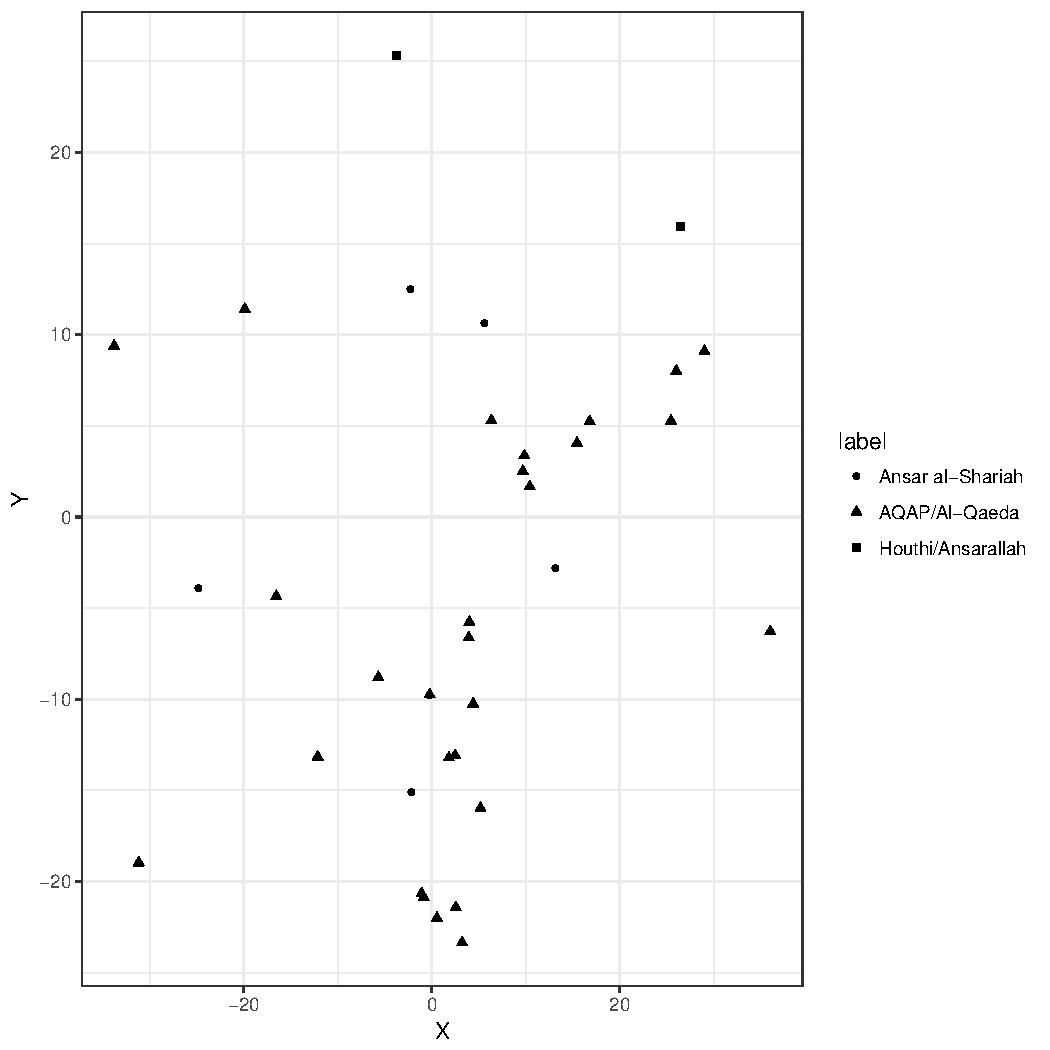
\includegraphics[width=.45\columnwidth]{./Pictures/2011DV_Panel_P50_tSNEDimRed.pdf}&
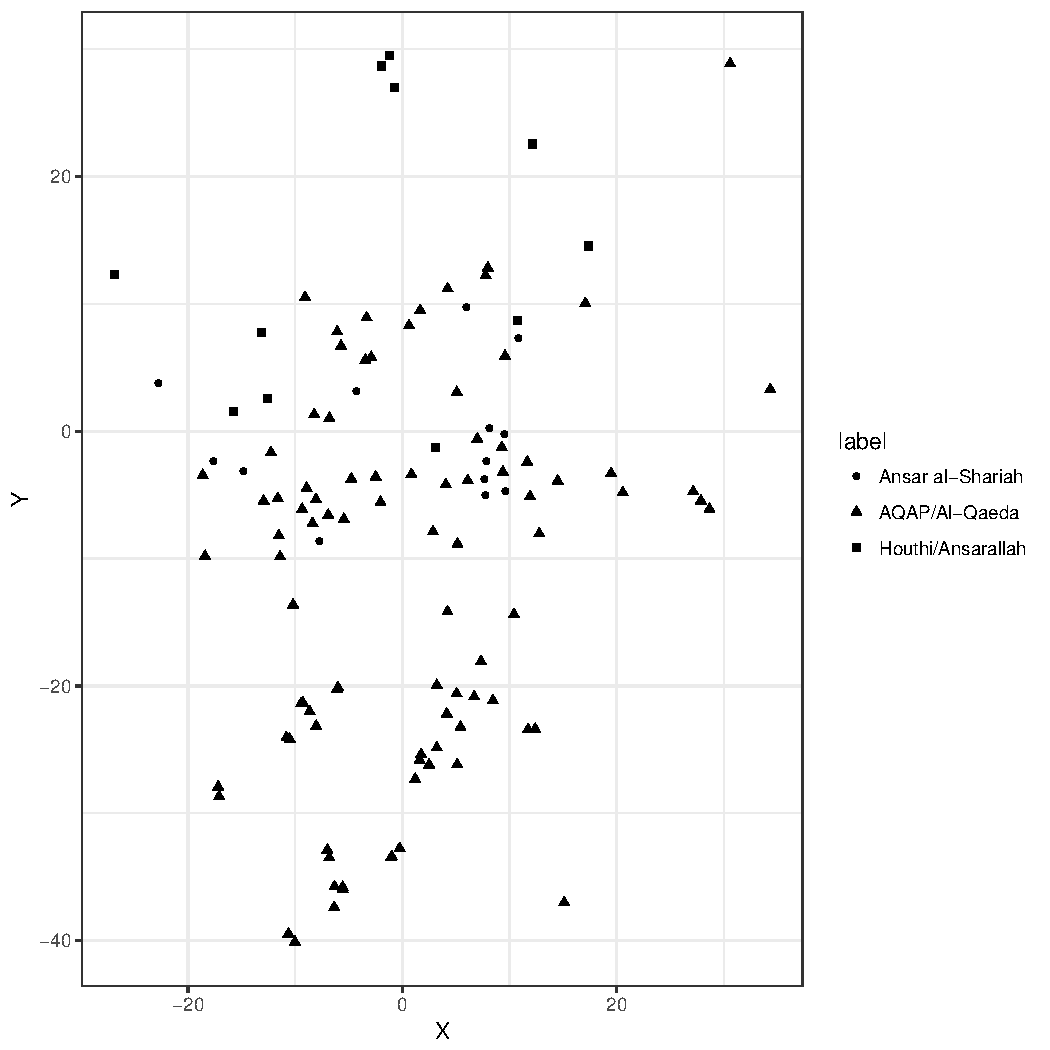
\includegraphics[width=.45\columnwidth]{./Pictures/2012DV_Panel_P50_tSNEDimRed.pdf}\\
 2011 & 2012\\
 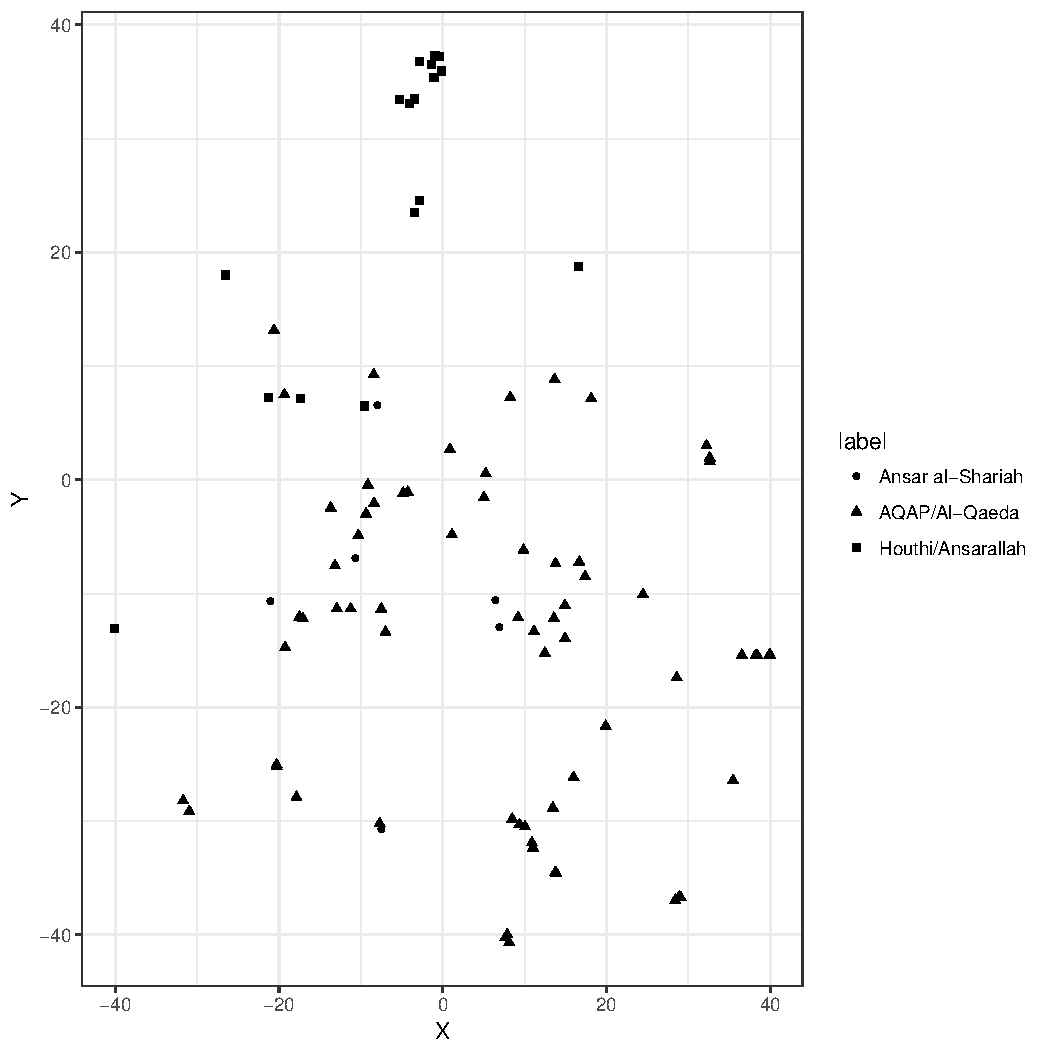
\includegraphics[width=.45\columnwidth]{./Pictures/2013DV_Panel_P50_tSNEDimRed.pdf}&
 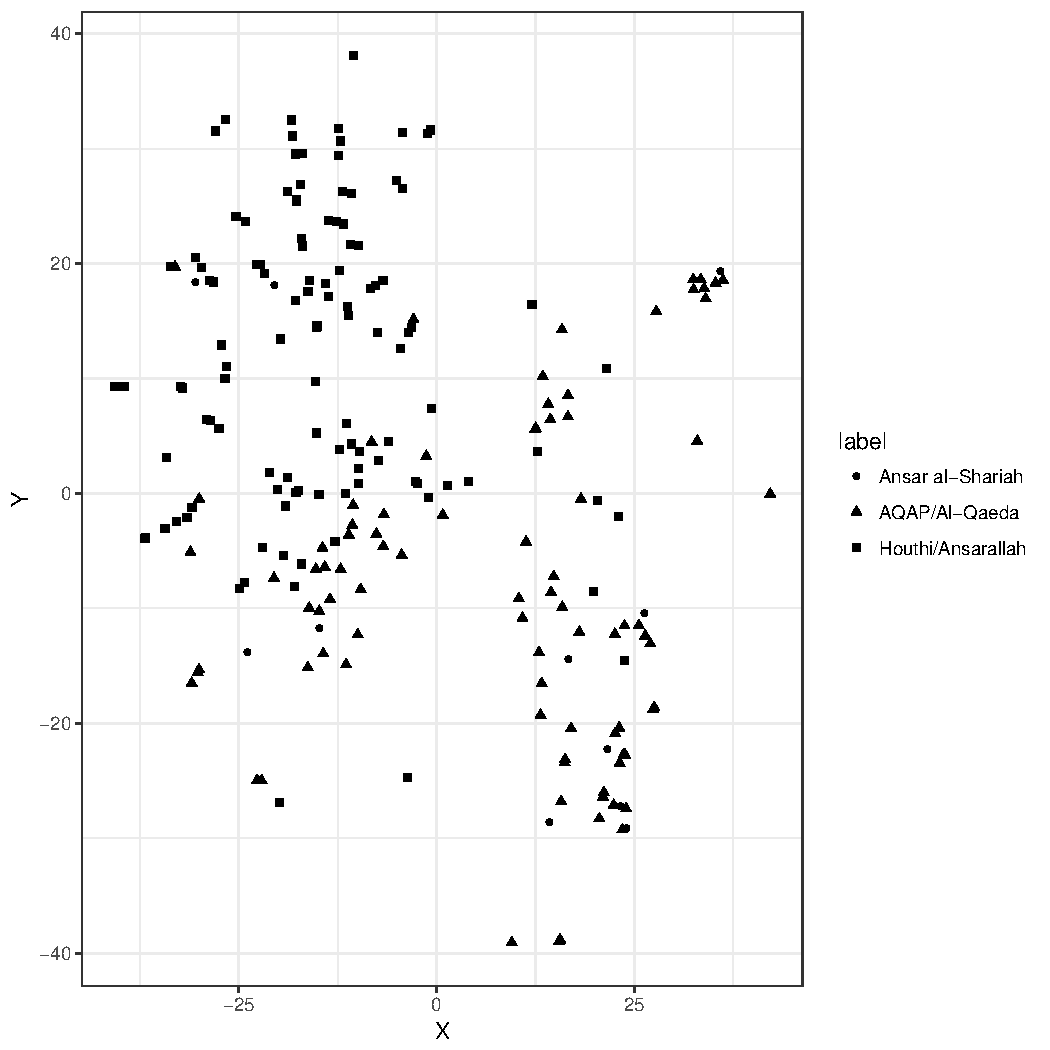
\includegraphics[width=.45\columnwidth]{./Pictures/2014DV_Panel_P50_tSNEDimRed.pdf}\\
  2013 & 2014\\
  \end{tabular}
  \caption{tSNE Clustering, All Stories 2011-2014}
  \label{fig:tSNE}
  \end{center}
  \end{figure}

The visualization presented here was generated by
running the t-SNE algorithm on for 5,000 iterations on the pooled
data. The perplexity hyperparameter presented below was selected after
grid sweeping from 5-50, at intervals of 5. Sweeping the perplexity
hyperparameter changes the exact outcome, as expected from a
probabilistic approach to summarizing structure in complex high
dimensional data, the conclusions are  broadly consistent across the
specifications. To address concerns that the observed clustering is random noise or driven by a specific
initialization, clustering was carried out in parallel on two
different machines using the same specifications but different
starting points. The results were broadly similar, namely  clear separation between the
Sunni and Houthi stories but lack of clear separation among stories
about AQAP and Ansar al-Shariah. As the diffusion and relative
positioning of clusters generated using t-SNE are not inherently
meaningful, comparison across the runs is only impressionistic and
presenting averaged results would not be meaningful.

Figure~\ref{fig:tSNE} presents t-SNE clustering for AQAP and Ansar
al-Shariah stories published between 2011 and 2014, presented
according to year of publication. These dates provide a snapshot of
writing about each of AQAP (green), Ansar al-Shariah (red), and the
Houthis (blue), and provide a high-level visualization of the
separation or convergence among the words used to describe each of the
three groups. The yearly clustering displayed in Figure~\ref{fig:tSNE}
features one point per story, and indicates that across the time
period, stories about the Houthi insurgency appear to be
systematically different from stories about the two Sunni groups, and
is suggestive of a pattern in which from 2012 through 2014, the Ansar
al-Shariah stories become progressively more similar to AQAP stories.
Figure~\ref{fig:tsne-sunnis} focuses only on whether or not the t-SNE
visualization differentiates between Ansar al-Shariah and AQAP
stories. As compared to the separation of the Houthi stories in the
corpus, the two Sunni groups demonstrate no apparent separation. This
implies that stories about the two groups are much more similar than
are stories about AQAP and the Houthi insurgency.   

\begin{center}
\begin{figure}
  \begin{tabular}{cc}
    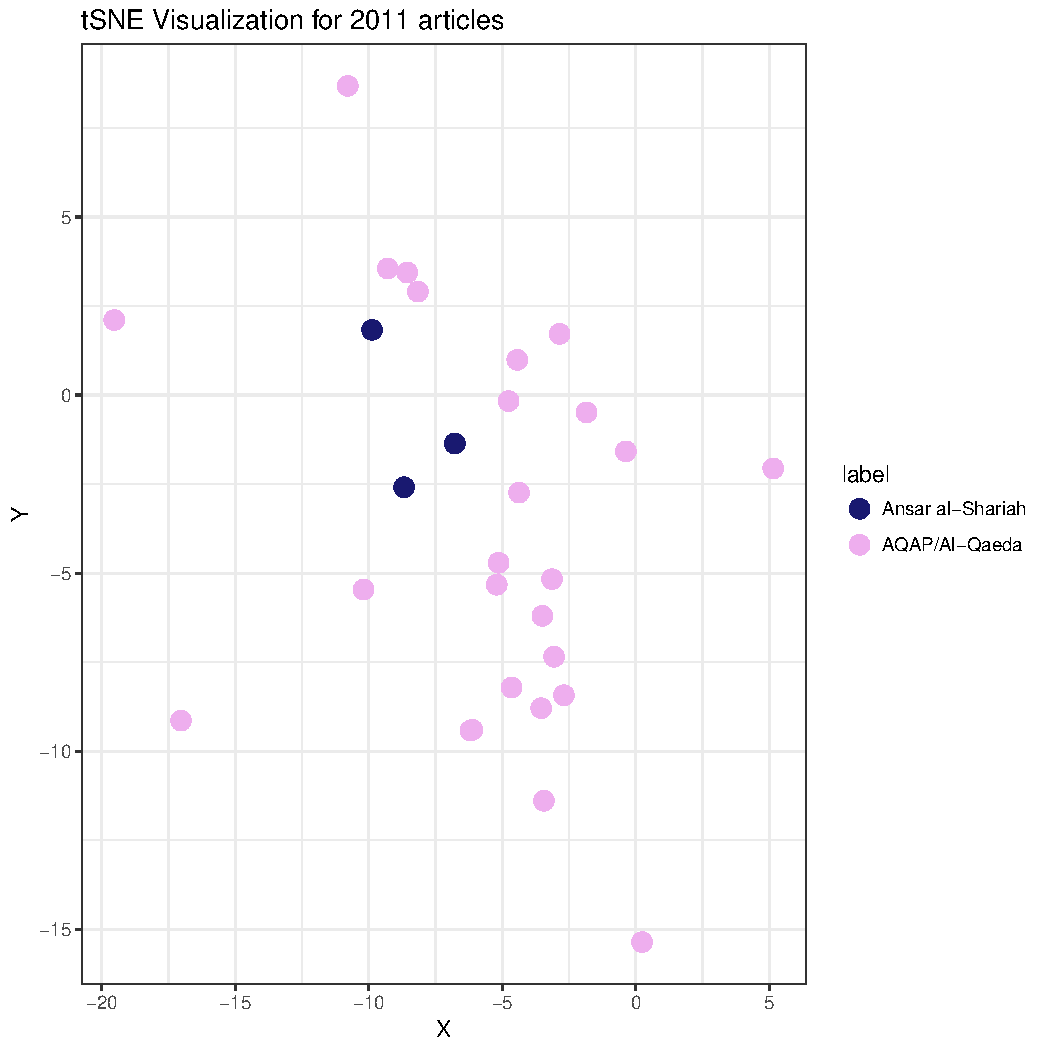
\includegraphics[width=.45\columnwidth]{./Pictures/2011sunnis_testData_tSNEDimRed.pdf}&
    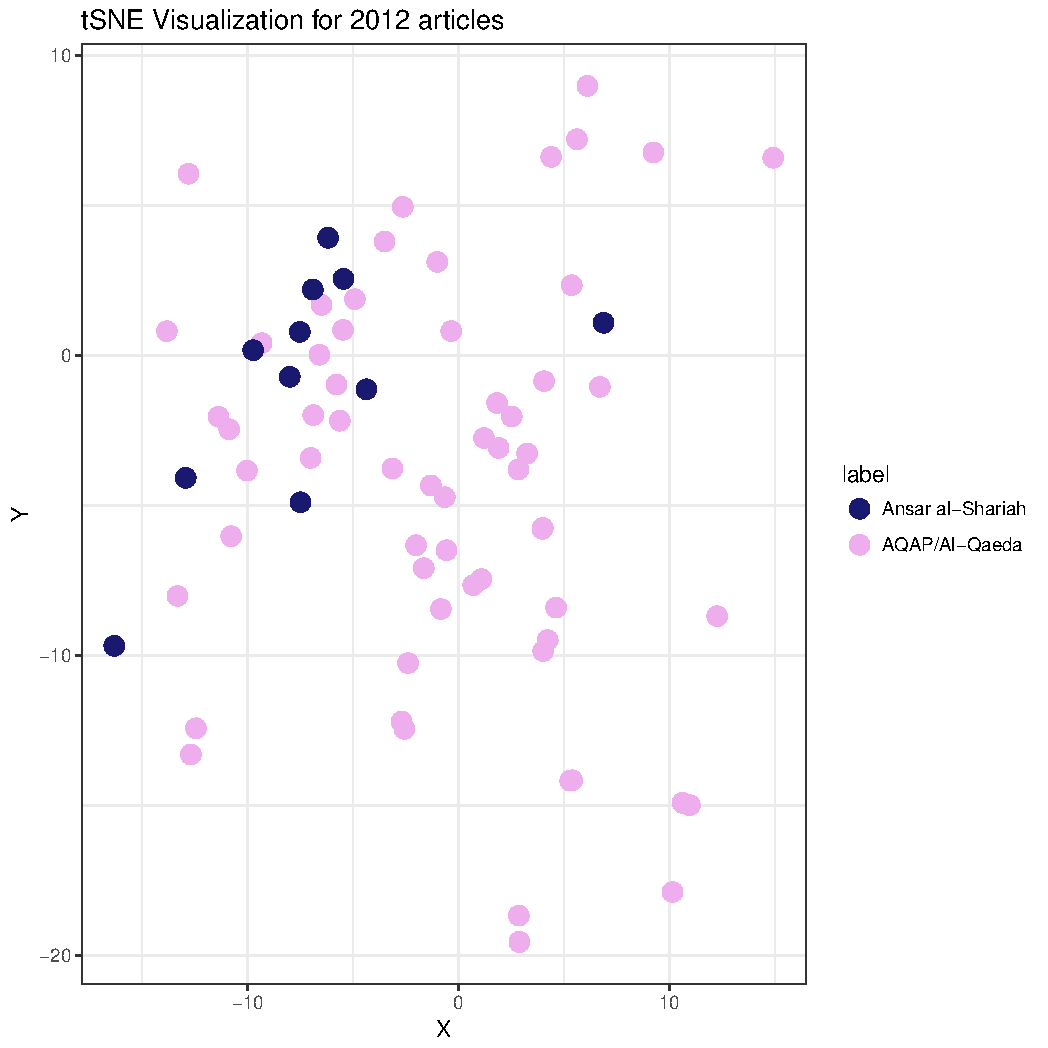
\includegraphics[width=.45\columnwidth]{./Pictures/2012sunnis_testData_tSNEDimRed.pdf}\\
    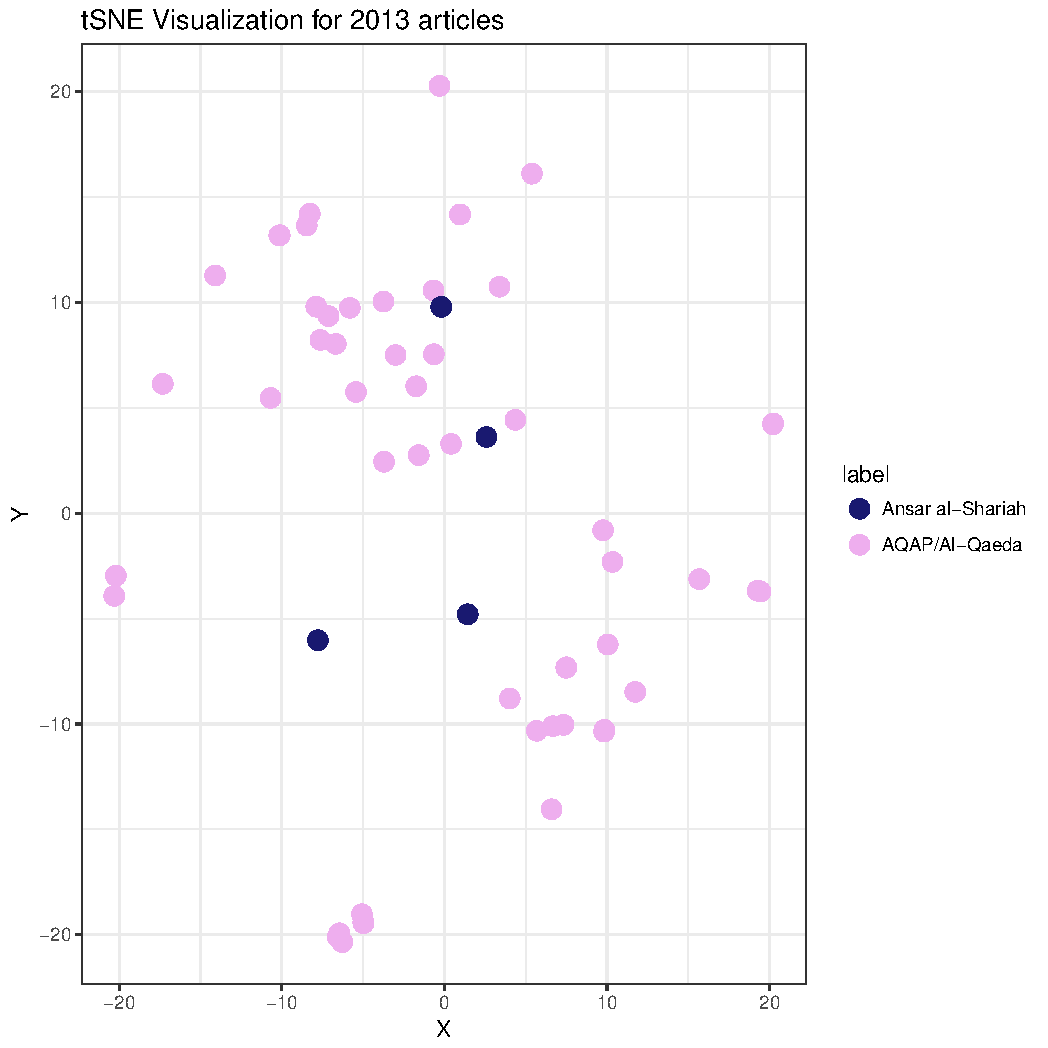
\includegraphics[width=.45\columnwidth]{./Pictures/2013sunnis_testData_tSNEDimRed.pdf}&
    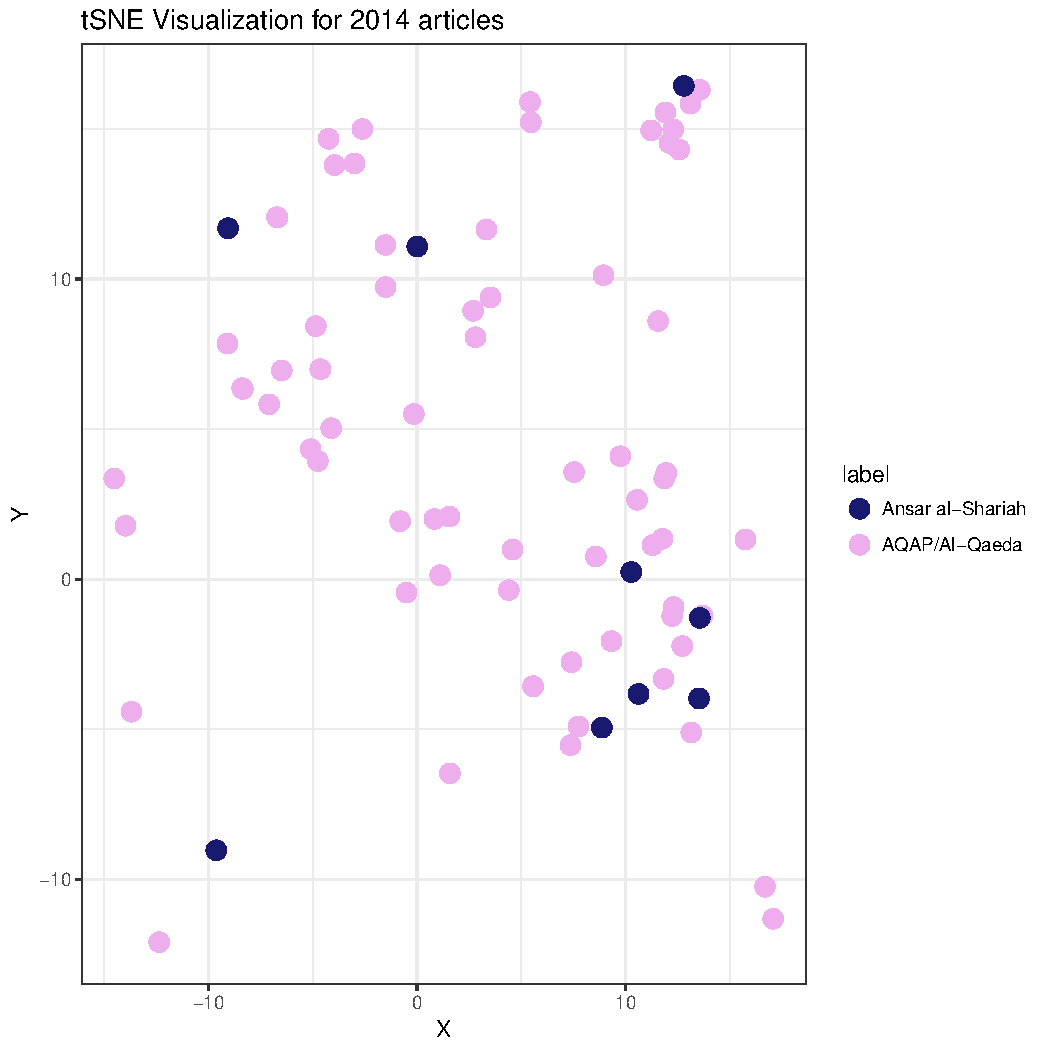
\includegraphics[width=.45\columnwidth]{./Pictures/2014sunnis_testData_tSNEDimRed.pdf}\\
  \end{tabular}
  \caption{tSNE Visualization Sunni Groups, 2011-2014}
  \label{fig:tsne-sunnis}
\end{figure}
\end{center}

\subsection{Random Forest Parameter Selection}

The random forest classifier used the randomforest() method from the
randomForest R package. The specification used the development data as training data, and the validation data as a test set, with story label as the classifier to predict. The confusion matrix for the training data is featured in the full text, while the confusion matrix for the training data appears below in Figure~\ref{tab:ref-conf-train}, followed by the classification results on the test data, in Figure~\ref{tab:ref-conf-test} .

The model grew 500 trees, from which is generated a proximity measure for each document. The variable importance plot was generated after extracting the variable importance measure and plotted using the varImpPlot() method native to randomForest. As the only predicted categories for the stories were AQAP and Houthi\/Ansarallah, the interpretation that
the random forest was identifying Houthi stories based on widespread description of the Shia group as a rebellion while the AQAP activities are more typically described as militant activity.

\begin{table*}[ht]
 \centering
 \begin{tabular}{rrrrr}
   \hline
  & AAS & AQAP/Al-Qaeda & Houthi & Class Error \\
   \hline
 Ansar al-Shariah & 0.00 & 24.00 & 2.00 & 1.00 \\
   AQAP/Al-Qaeda & 4.00 & 240.00 & 3.00 & 0.03 \\
   Houthi/Ansarallah & 0.00 & 7.00 & 152.00 & 0.04 \\
    \hline
 \end{tabular}
 \caption{Random Forest Confusion Matrix, Training Data}
\label{tab:ref-conf-train}
 \end{table*}
 
 
 \begin{table}[ht]
 \centering
 \begin{tabular}{rrrrr}
   \hline
  & AAS & AQAP/Al-Qaeda & Houthi & Class Error \\
   \hline
 Ansar al-Shariah & 0.00 & 6.00 & 3.00 & 1.00 \\
   AQAP/Al-Qaeda & 0.00 & 48.00 & 19.00 & 0.28 \\
   Houthi/Ansarallah & 0.00 & 14.00 & 25.00 & 0.36 \\
    \hline
 \end{tabular}
\caption{Random Forest Confusion Matrix, Test Data}
\label{tab:ref-conf-test}
 \end{table}
  
 
\begin{figure}
\begin{center}
\begin{tabular}{c}
  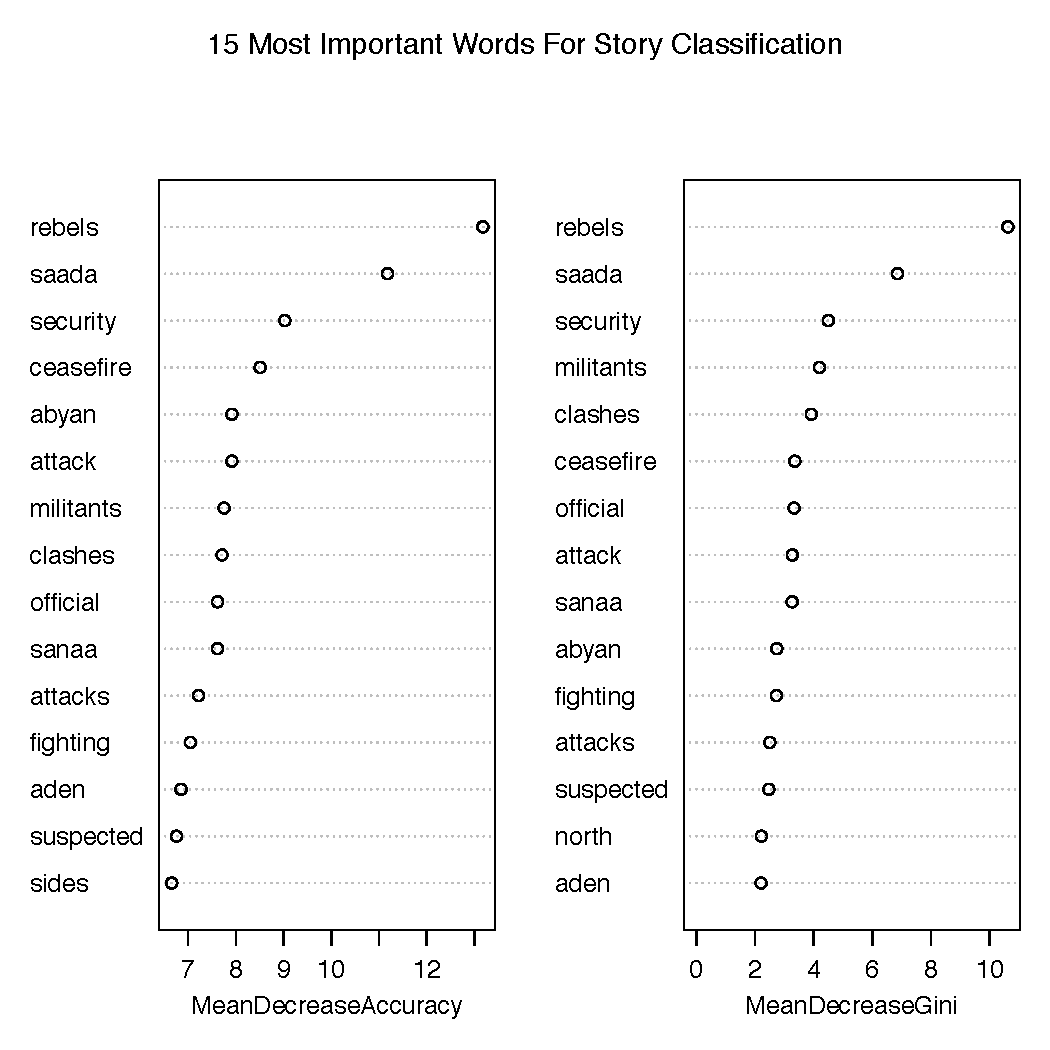
\includegraphics[width=5.00in]{./Pictures/randomForestRes.pdf}\\
\end{tabular}
\caption{Important Words for Classification}
\label{fig:rf-impt}
\end{center}
 \end{figure}

A second version of the random forest model estimated the model only on Ansar al-Shariah and AQAP stories. As with the full data, this
model failed to predict any stories for the Ansar al-Shariah
label. However, it did predict two AQAP-labeled stories as being
likely Ansar al-Shariah stories. These stories were an August 3, 2014
story about a clash between al-Qaeda militants and police forces and a
December 17, 2014 story about a car bomb carried out against Yemeni
police officers. Notably, both stories were one of the 11 stories from
Xinhua News that used the names AQAP and Ansar al-Shariah
interchangeably.

One advantage of the random forest approach to classifying text is that the features
used for classification are also terms in the document, which provide
interpretable insights into what words drive separation among stories
in the data. The fifteen most important words for the random forest
classification---after removing stopwords that describe or name the
active group--- suggest that the reason for the clean split
across the Sunni and Shia movements lies in framing. The list of these
terms, ranked in order of their importance for decreasing the
classifier accuracy (left) and importance for decreasing homogeneity
in the final nodes of the classification (right), can be seen in
Figure~\ref{fig:rf-impt}. The importance of \say{rebels} as the top term
for both accuracy and Gini coefficient is revealing: indeed in the
texts, Houthis are consistently described as \say{rebels} while the Sunni fighters are
frequently presented as \say{militants.}  After the rebel/militant
split, words that describe the location of operations and military occupations are, unsurprisingly, important classifiers:  Aden, Saada and Sanaa are
regions associated with Houthi territorial gains, while Abyan is more
closely linked to AQAP and Ansar al-Shariah
activities.

\subsection{Principle Component Analysis}

Another view of the separation among the stories is shown in
Figure~\ref{fig:rf-pca1}, which uses a principle component analysis (PCA) to
plot proximity of stories, as measured by the proportion of times that
individual stories are in the same terminal
node~\autocite{jones2015exploratory}.  This reaffirms the takeaway from
the confusion matrix: Houthi stories are distinct from AQAP stories,
but Ansar al-Shariah stories contain enough words in common with AQAP
stories that the two are difficult to distinguish via the random
forest's iterated decision trees.

\begin{figure}
\begin{center}
\begin{tabular}{c}
 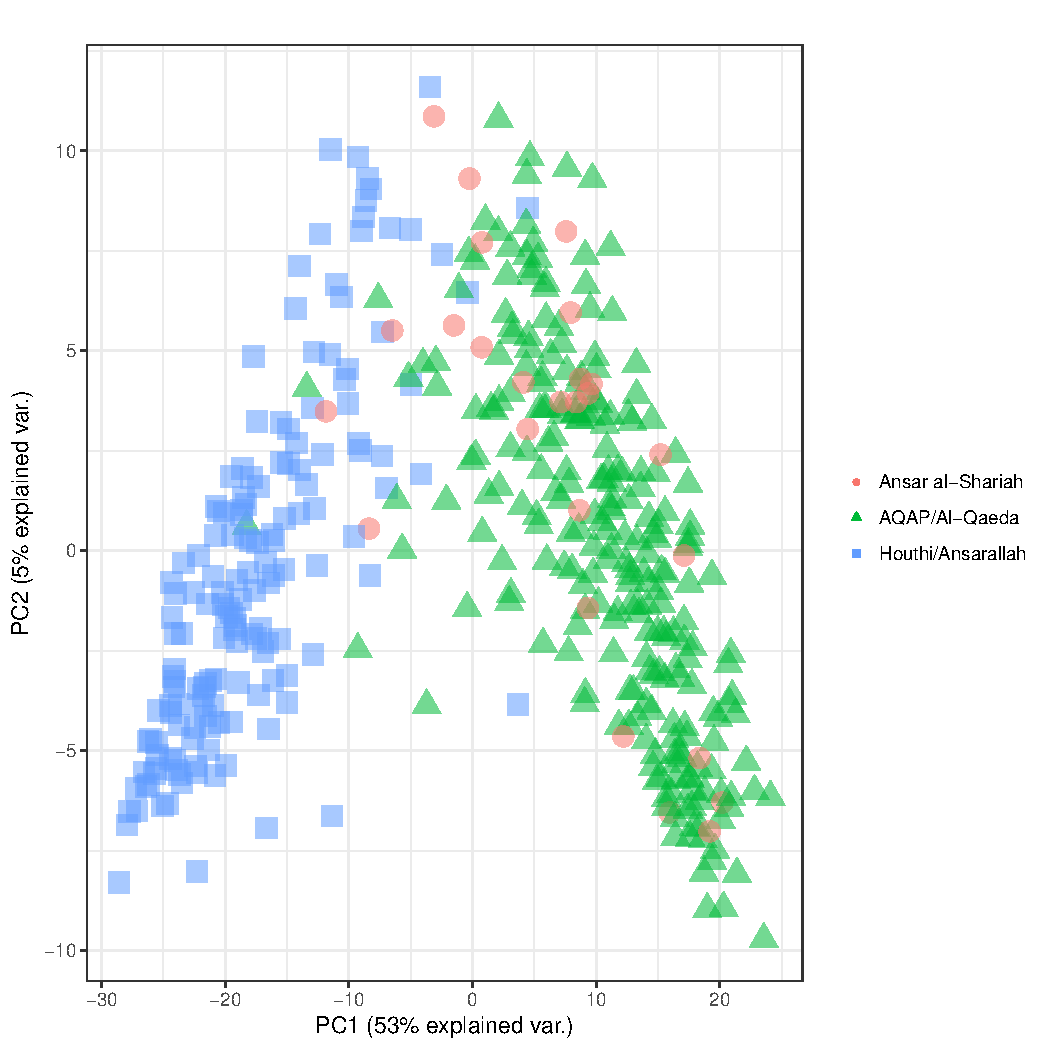
\includegraphics[width=5.00in]{./Pictures/pca_proximityRF.pdf}
\end{tabular}
\caption{PCA Visualization of Group Classification}
\label{fig:rf-pca1}
\end{center}
 \end{figure}

The principle component analysis presentation was done using the
extract\_proximity() and prcomp() methods from the edarf R
package. The proximity extraction categorizes document proximity as
the proportion of times that two observations are in the same terminal
node across each estimated tree. This generates an NxN matrix of
location similarities.  This proximity is visualized using a principle
components analysis of the proximity matrix, implemented in the edarf package.

\subsection{SVM Specification}

The support vector machine classification was developed using the
ksvm() method from the kernlab R package. I used the ``development''
data as a training set and the ``validation'' data as the test set,
with ``label'' as the classification attribute to predict and the
words from each term document matrix as the features used in the
classification.
The kernel specified was the radial basis function (RBF) Gaussian
kernel via kernlab's ``rbfdot'' implementation. The RBF kernel is
defined as:$K(x,x\prime)=$exp$(-\frac{||x-x\prime||^{2}}{2\sigma^{2}})$. This
kernel is based on squared Euclidean distance between feature vectors
for each document, and thus is amenable to interpretation as distance
between the documents. The svm carried out a 3-fold cross-validation
on the test set, and used the resulting model to predict category
assignment in the test (validation) set. In the analysis presented in
the paper, each class was given a weight of 1.  The paper reports
predicted probability of label assignment.

Given the imbalance in the data, I developed two additional versions of
the SVM model, subsetting the  development-validation data subset to include only AQAP and Ansar al-Shariah stories. One of these replicated the
original support vector machine with an equal weighting on each
possible class and one of which assigned class weights to the
labels in the 90-10\% distribution of AQAP and Ansar al-Shariah
stories.  Results of these two models were similar to the model
presented in the paper: given the words in
the news stories as features, the SVM does not distinguish Ansar
al-Shariah stories from AQAP stories.

Figure~\ref{fig:svm-mis} provides a closer look at whether the
support vector machine's confidence in whether to assign stories to
Ansar al-Shariah or AQAP change over time. Ideally, support for the
transformation theory would indicate the SVM assigning increasing weight to the Ansar
al-Shariah label for news stories about AQAP activities as AQAP
members push the group to engage with local concerns.  The plot
focuses on stories with a true label of AQAP and depicts the predicted
probability that an article would be assigned to the label of Ansar
al-Shariah given that it is a story about AQAP actions (red) as well as the
SVM's confidence in the classification for AQAP (blue) for the 144
stories in the test set. As the SVM consistently predicts all AQAP and
Ansar al-Shariah stories for AQAP, the expected probability of
assignment to Ansar al-Shariah remains constant at approximately
$p=.15$. The classification predictions provide mixed support for the
expectation that an influx of local members should increase the
difficulty of assigning group labels: although the SVM's confidence in
predicting the AQAP label becomes more variable over time, the
predicted probabilcde fg
issignmentcde fg
sar al-Shariah remains
constant over the time period

\begin{figure}
\begin{center}
\begin{tabular}{c}
  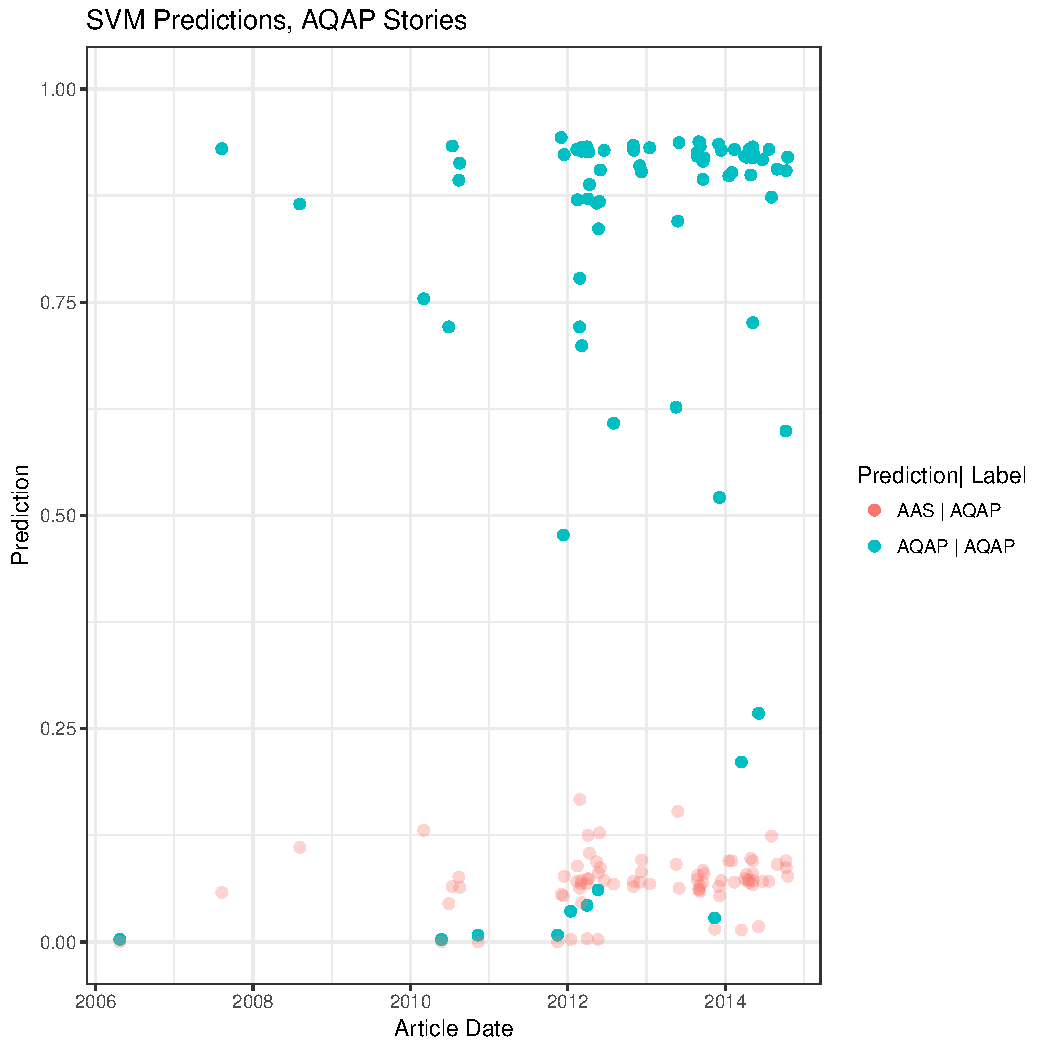
\includegraphics[width=5.00in]{./Pictures/PredictedProbabilities_AQAPPreds.pdf}\\
\end{tabular}
\caption{SVM Predictions Over Time For AQAP Stories}
\label{fig:svm-mis}
\end{center}
\end{figure}

\section{Structural Topic Model}

The three STM models are based on a corpus of 1353 documents, spanning October
25, 2005 through September 21, 2016. Approximately 500 documents are
associated with as-Sahab. A histogram of the distribution
of can be seen in Figure~\ref{fig:hist}. 

\subsection{Document Pre-processing}

I focus on media released online to jihadi media platforms and
outlets.  Preprocessing removed words that occurred in fewer than two or more 70\%
of the documents in the corpus.\footnote{In the AQAP corpus, there was
no change to the number of tokens in the corpus for an upper bound
threshold between 70-95\%. I evaluated coherence and exclusivity at
an upper threshold of 50\%, but did not find results that would
suggest either a coherence or exclusivity benefit from the additional
reduction in corpus size.}

\begin{figure}
\begin{center}
  \begin{tabular}{c}
    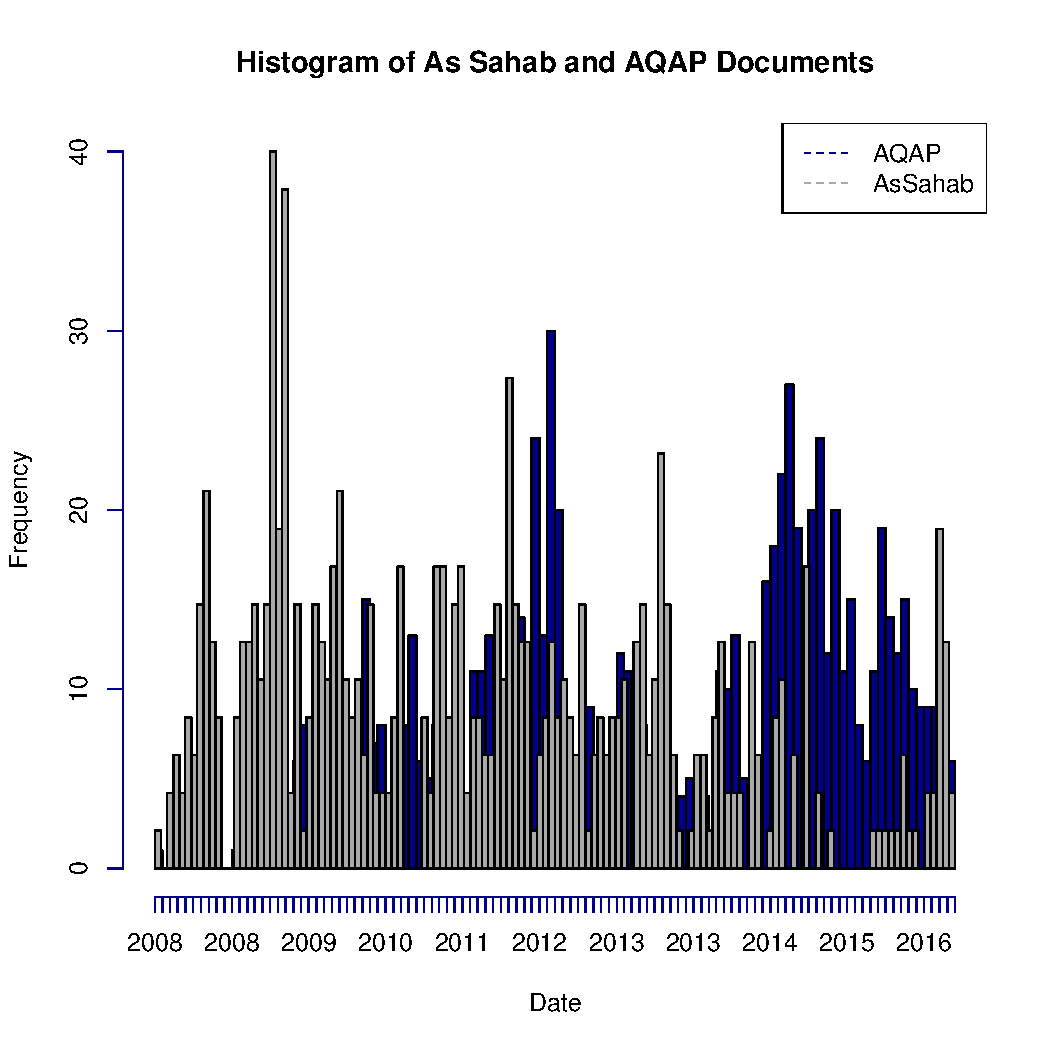
\includegraphics[width=5.00in]{./Pictures/histofAQAPandAS.pdf}
  \end{tabular}
  \caption{Distribution of AQAP and AQC Materials}
  \label{fig:hist}
\end{center}
\end{figure}

Models One, Two, and Three each use time as a covariate. The time
variable is expressed in the data as a running counter of days from
the oldest document in each corpus. Thus, the date of the oldest
document is given as 1 and the \say{day} of each subsequent document is
modeled as the numer of days between the first date and the date of
the individual document. These dates are linked to the                                                           
  translation date rather than release date as the former can be                                            
  accurately pinpointed for each document in the corpus. For the vast                                       
  majority of the corpus, the translation date closely coincides with                                       
  the date that the document was released to online jihadi media outlets. The precision                     
  of release dates contained in the original Arabic text can vary                                           
  according to type of document: communiques are typically dated                                            
  to a specific day, while strategy documents or promotional magazines                                      
  can be dated with a day, a month, or even a season. Thus, for                                             
  consistency, the date covariate is linked to translation date.

\subsection{Model Selection}
Topic models rely on the user to prespecify a number topics for the
algorithm to search for. However, this parameter fundamentally influences the themes that will be
identified in the documents.  For models one and two, I selected the number of topics by doing a
sweep of model specifications with 10 to 30 topics. I selected a
topic number that performed best on both semantic coherence and
exclusivity.\footnote{Ideally, the selected number of topics would
  have relatively high exclusivity and semantic coherence. I often
  faced a trade-off between the two. When determining the trade-off, I
  prioritized semantic coherence over exclusivity. The exclusivity bands were, overall, narrow while
coherence varied substantially.} After this process, a model with 18 topics
appeared to present the greatest gains to semantic coherence without
trading off exclusivity. Moreover, the 18-topic model identified
topics that were particularly substantively coherent. 

For the joint model, after comparing the semantic
coherence-exclusivity trade-off for models across a sweep from 10
to 40 topics, I set the number of topics to discover at
34. The increase of topics reflects the expectation that the two
organizations are already rhetorically distinct, and so the joint
corpus should require more topics. Specifically choosing an output
that doubled the number of topics slightly penalized semantic
coherence over a model with fewer topics, but allowed for a more
precise comparison of topics between each group. 

As topic models are, by nature, non-deterministic, each
implementation of a given model will produce slightly different
results. Thus, after selecting the number of topics for the STM to
identify, I ran each model specification ten times to create a range of
possible output models for analysis. I compared the average
semantic coherence and exclusivity for each of the models. For each of
the three models below, I found that the averages within each
ten-model set were nearly identical. To avoid biasing my results by
selectively choosing the output that best confirms my theoretical expectations, I chose
which specific models to analyze by maximizing average coherence
and exclusivity metrics. As no model clearly dominated the
coherence-exclusivity trade-off, I assigned a relatively stronger
weighting to semantic coherence when selecting a specific iteration to
present. I then selected a model to present before qualitatively evaluating any of the topics. This
decision was intended to avoid bias in choosing how to prioritize
coherence gains against exclusivity losses.\footnote{A plot of average
semantic coherence and exclusivity scores is available upon request.} 
 
Finally, after selecting which model to present, I evaluated the
remaining models to ensure that the output was consistent across the
set of ten results for each model. In particular, I verified general
agreement on the thematic content identified across the runs.

% \subsection*{Choice of topic number}
%% [Ed note: commented out until I figure out if k=17 here was a typo
%% or if I had a reason to say that K=17 had highest semantic
%% coherence, but I went with k=18]

% I set the number of topics with reference to balancing semantic
% coherence, exclusivity, and held-out likelihood of models varying
% values of K. Exclusivity was in a narrow range for both the AQAP and
% As-Sahab corpus, so I placed most weight on semantic coherence.

% For AQAP documents, k=17 is clear winner for high semantic coherence,
% but has among lowest exclusivity. Next best are the 34, 36, 39
% cluster. They have highest exclusivity and in top 9/40 coherence. 

% \begin{center}
% \begin{table}
%   \begin{tabular}{cc}
%     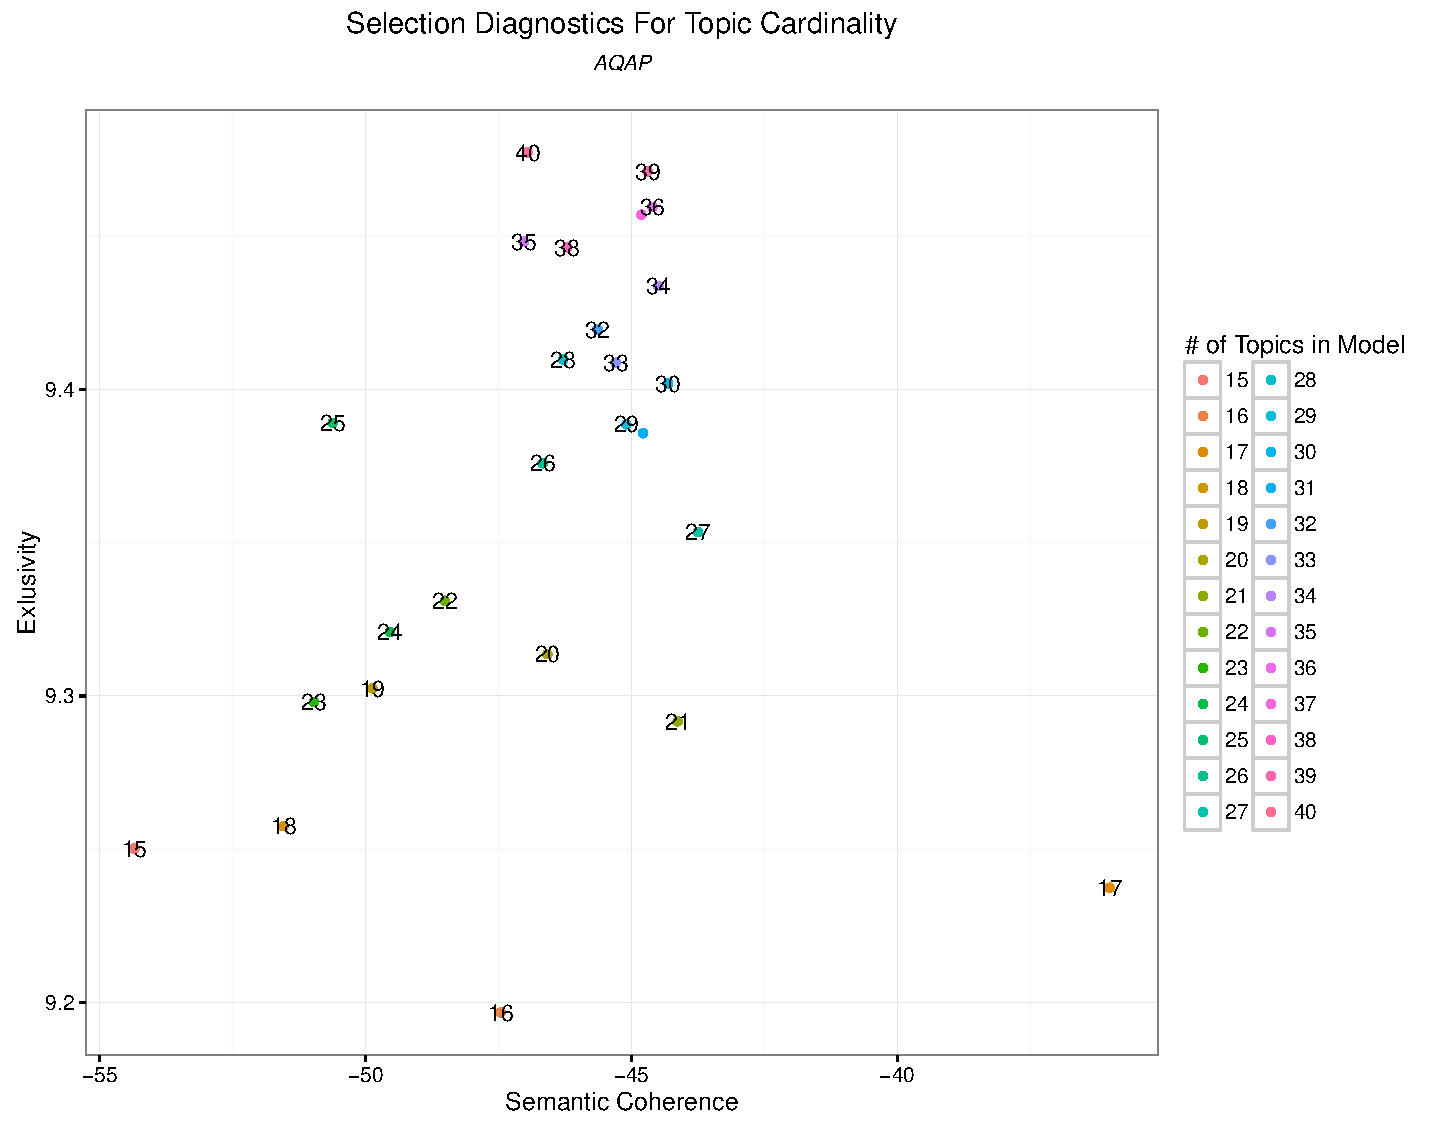
\includegraphics[width=3.00in]{aqapAQAPKSelectSummary.pdf}&
%     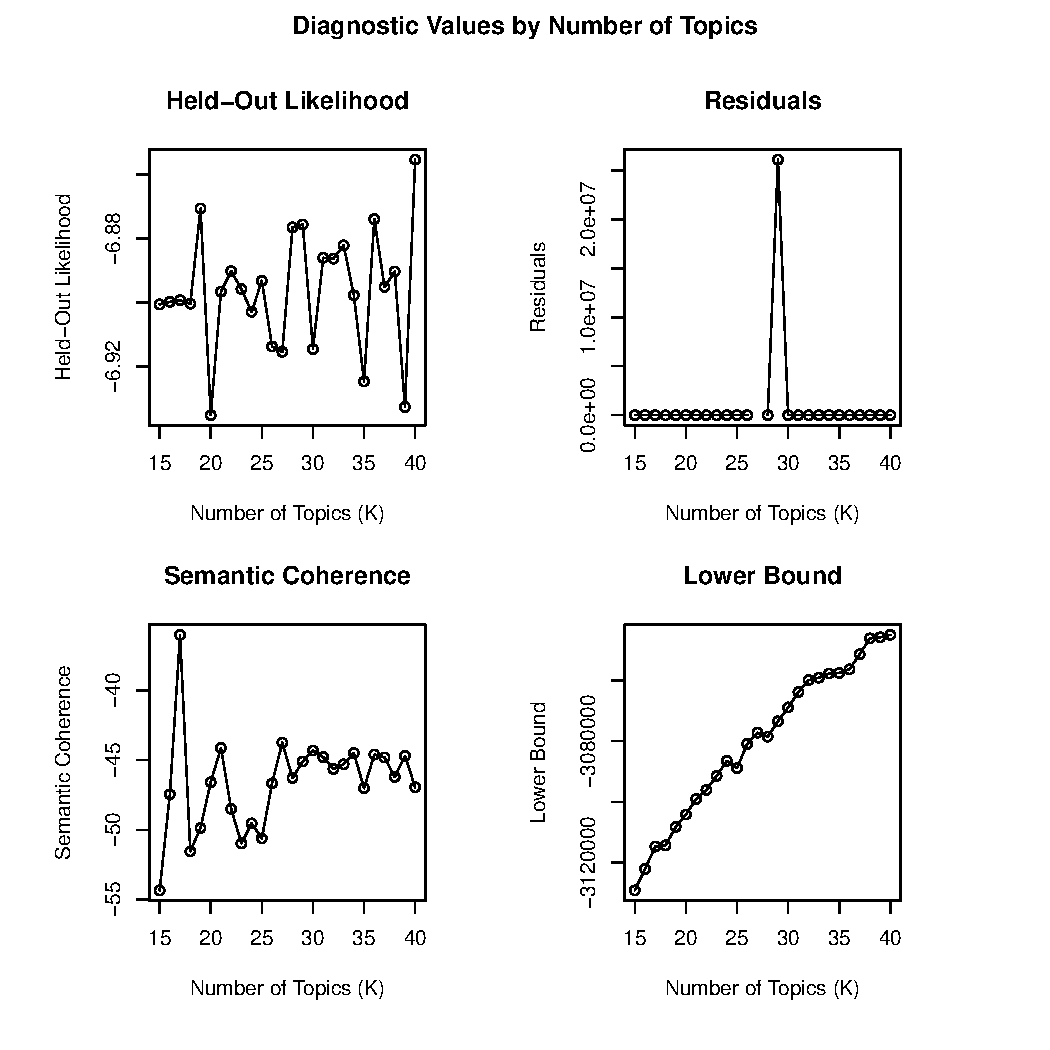
\includegraphics[width=3.00in]{aqapbaseDiagnosticPlot.pdf}
%   \end{tabular}
%   \caption{Model Diagnostics for AQAP Corpus}
%   \label{tab:aqapdiag}
% \end{table}
% \end{center}

% For as-Sahab, k=15, 16, 17, and 18 are all tightly clustered at the
% highest end of coherence. The range for exclusivity is particularly narrow, so I put most of the selection weight on semantic coherence.
% \begin{center}
% \begin{table}
%   \begin{tabular}{cc}
%     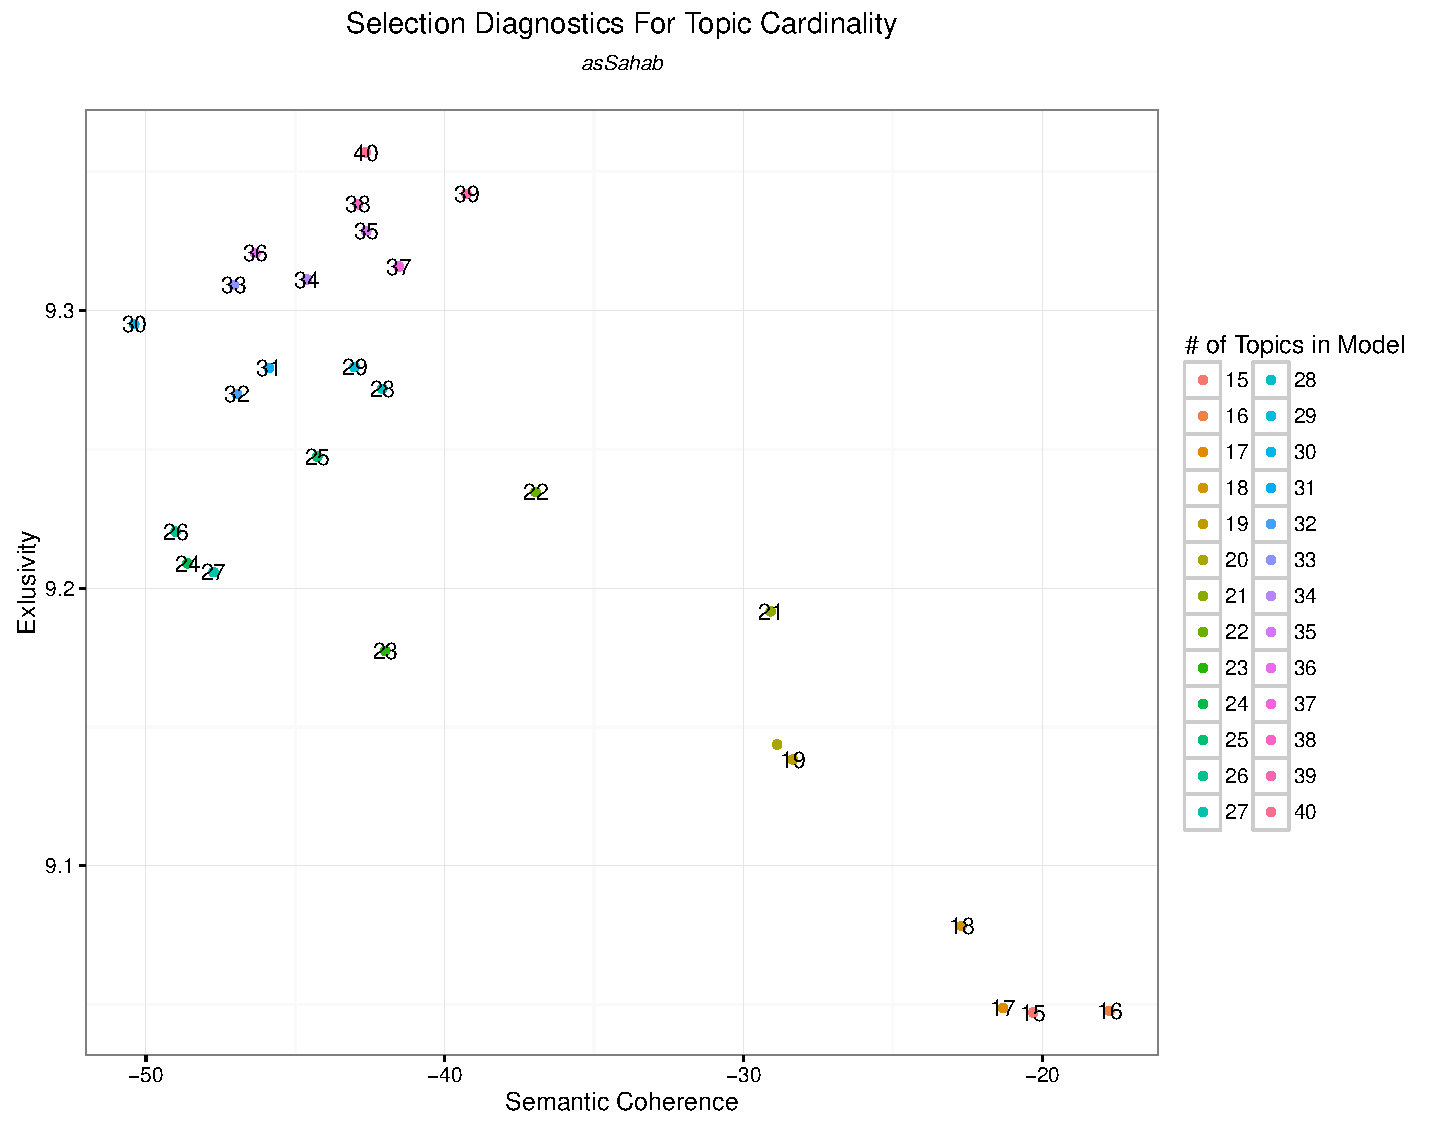
\includegraphics[width=3.00in]{asSahabAQAPKSelectSummary.pdf}&
%     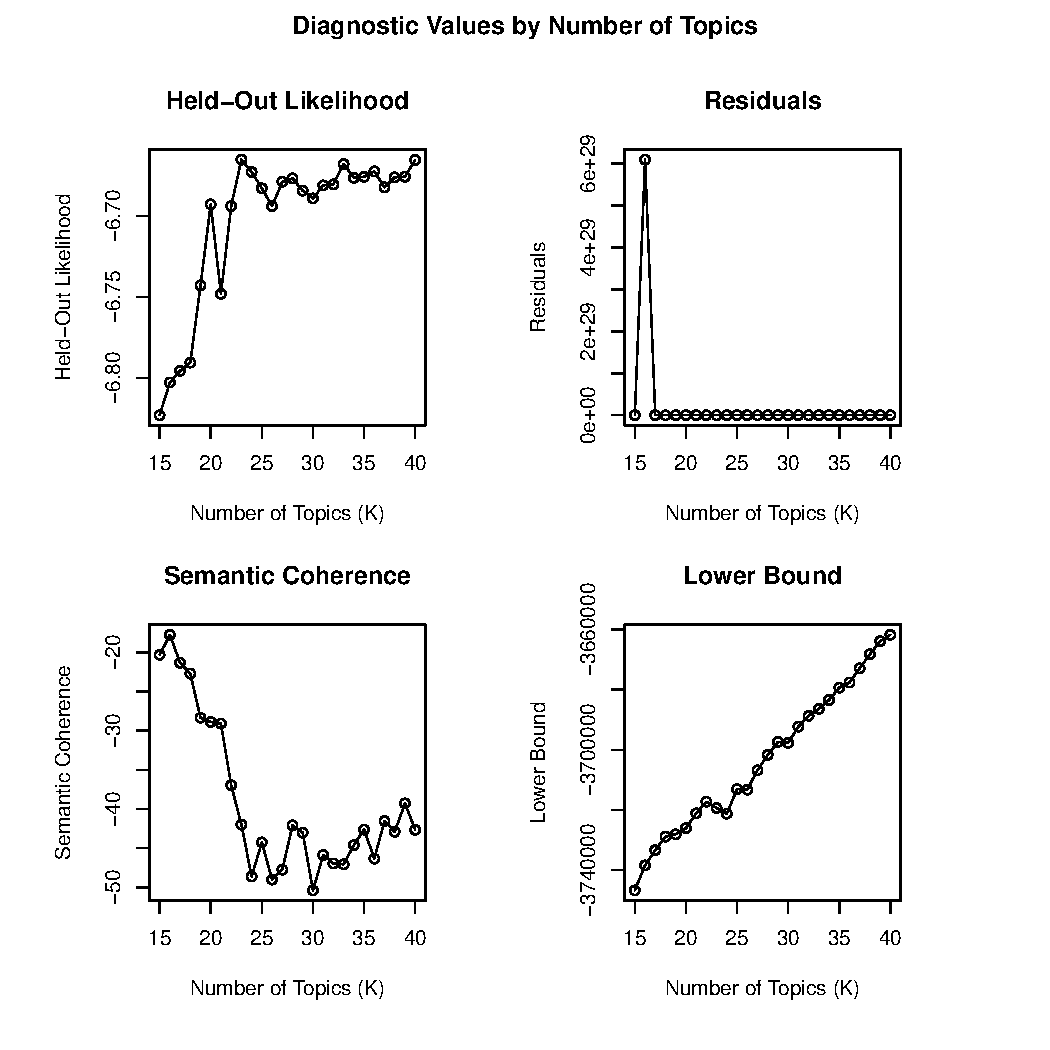
\includegraphics[width=3.00in]{asSahabbaseDiagnosticPlot.pdf}
%   \end{tabular}
%   \caption{Model Diagnostics for as-Sahab Corpus}
%   \label{tab:asbdiag}
% \end{table}
% \end{center}

%% \underline{Additional topics in Model One}\\

%% The two remaining Yemen-centric topics are topics 3 and 11. Topic 3, labeled as the
%% ``Southern Yemen'' topic strongly relates to AQAP's 2011 seizure of territory in the
%% south of the country during the 2011 Revolution. The topic rises in
%% prominence while the organization controlled territory in 2011 and
%% 2012, and then quickly recedes as an expected thematic topic.  As
%% such, the topic is a useful indicator that the STM model identified
%% are reflective of underlying events.  footnote{The third Yemen-related
%%   topic, loosely named the ``US in Yemen'' topic, does not has as
%%   clearly interpretable thematic structure as do the other three
%%   Yemen-centric topics, and so is not presented here.}

 Figure~\ref{fig:civsandfactions} depicts the expected proportion
of the transnational jihadi topics presented according to
time.\footnote{For interpretability, the x-axis is labeled by year. The model was
  estimated according to the number of days from the start of the
  document corpus.}  The y-axis represents the expected proportion of
each document dedicated to each topic. For context, I added four
vertical lines marking important dates identified above. From left to right, the
lines represent: the al-Majalah airstrike on December 17, 2009; the start of
the Yemeni Revolution on January 27, 2011; the death of Usama bin
Laden on May 2, 2011; the end of the first Obama Administration on
January 19, 2012; and the Houthi takeover of Sanaa on September 21, 2014.

\subsection{Local Conflict Topics}

The \say{Local Conflict} cluster is comprised of four STM-identified topics. The topics are unified by a shared focus on people and places local to Yemen, as well as tactical terms that suggest military operations.  

Within the cluster, specific topics are internally unified by their focus. One topic, which I have named \say{Southern Yemen} is characterized by geographic references to Abyan Governorate, which was held by Islamic militants in 2012.  Another, the \say{Local Targets} topic has a geographic focus on Hadramawt Governorate in Central Yemen and makes frequent references to specific operational behaviors and targets. The \say{Houthis} local topic combines frequent temporal references with military terms, a combination that is indicative of claims of military operations.

Figure~\ref{fig:houthisLT} shows temporal trends in the expected proportion of the corpus dedicated to each of the four topics in the \say{Local Topics} cluster. Notably, the \say{Houthi} and \say{Southern Yemen} topics closely track then-current events. Each topic rises in prevalence in the corpus corresponding to the dates of the respective military offensives. Moreover, that the unsupervised topic model \say{discovered} the military offensives provides a useful source of external validity for the 18-topic model.

\begin{figure*}
\begin{center}
\caption{Changes over time to attention dedicated to local topics}
  \label{fig:houthisLT}
  \begin{tabular}{c}
    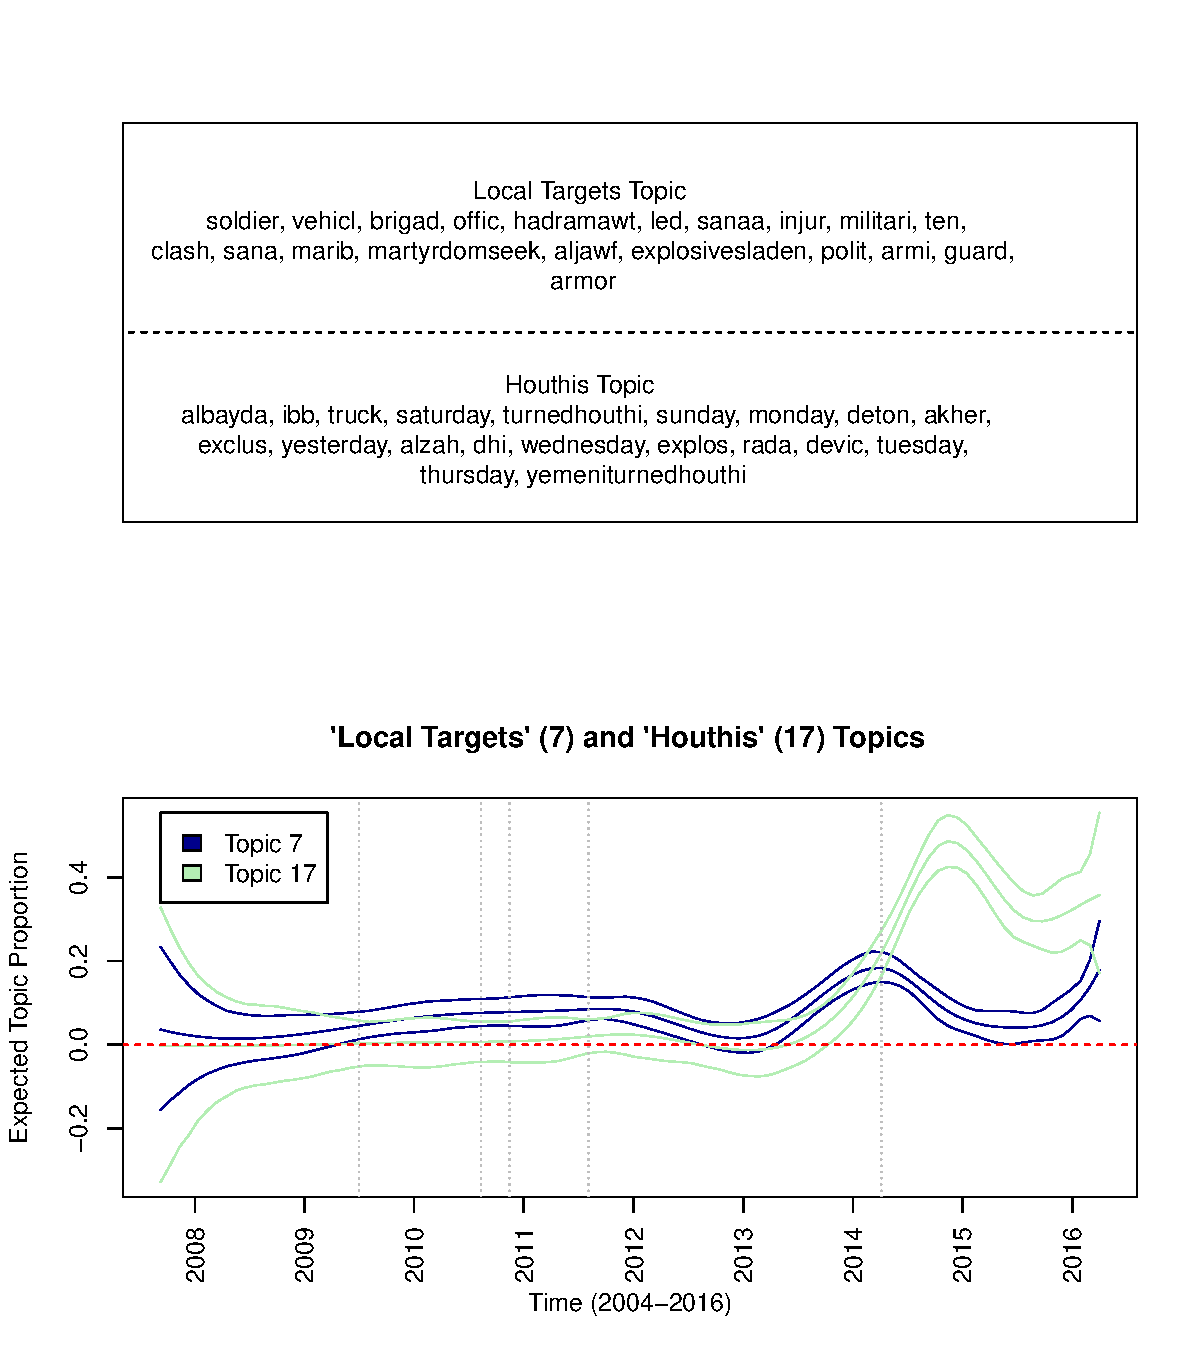
\includegraphics[width=.65\columnwidth]{./Pictures/HouthiandLT_UT7_K18.pdf}\\
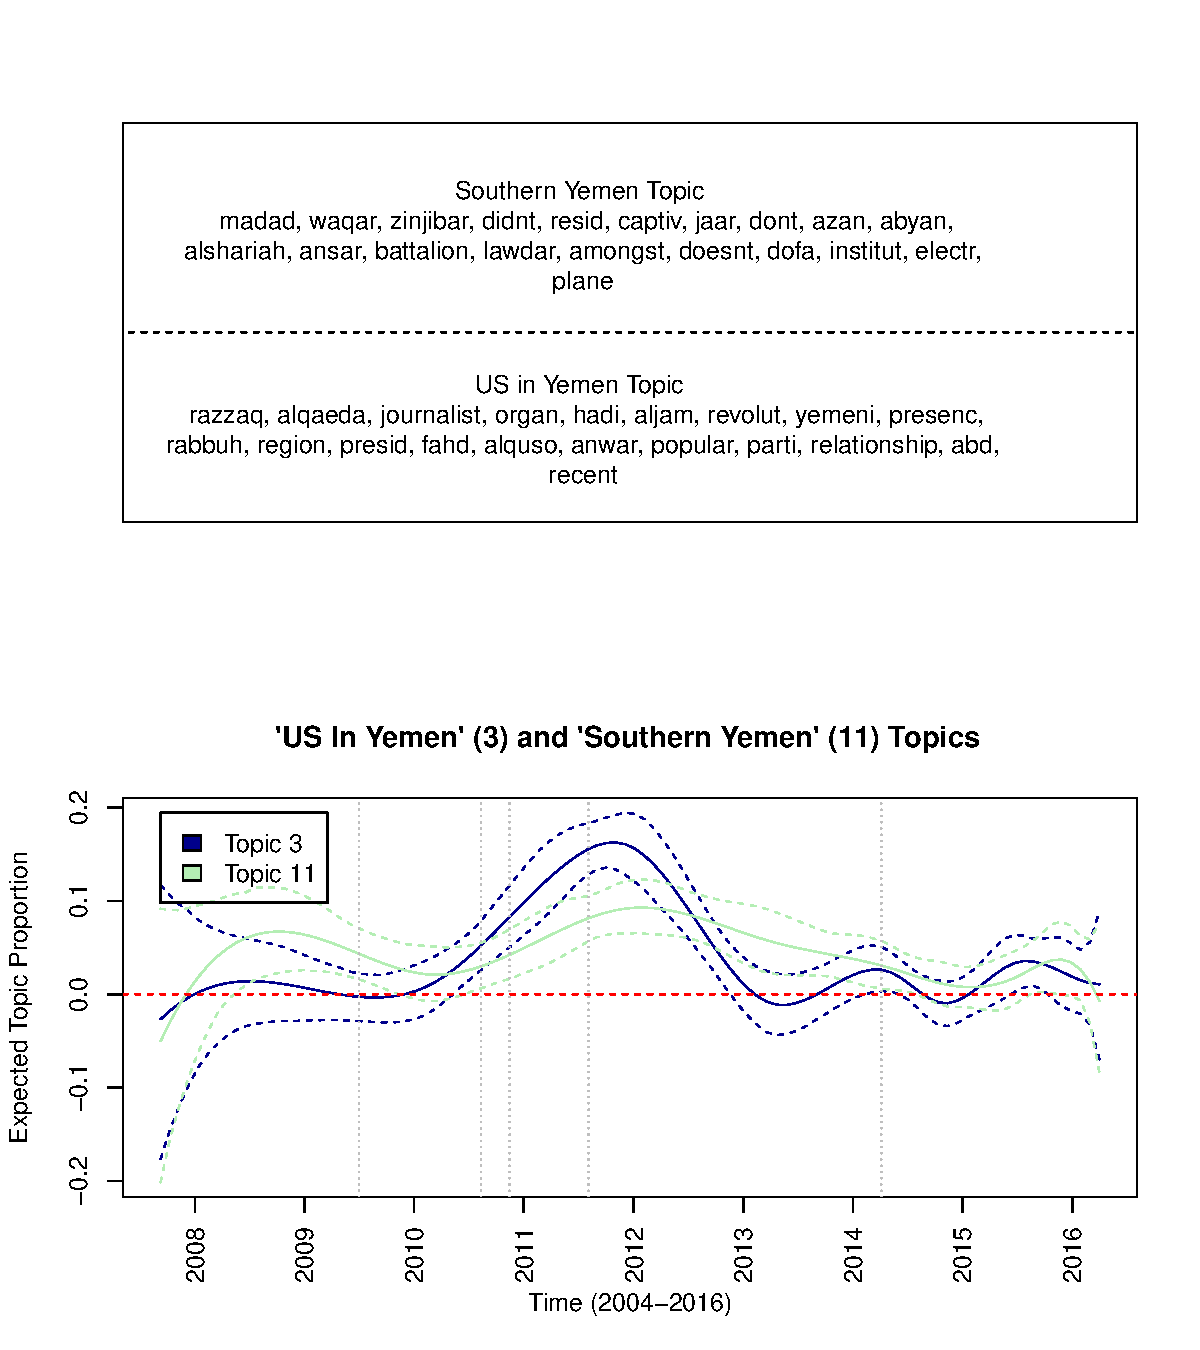
\includegraphics[width=.65\columnwidth]{./Pictures/AASAndMiscYemen_UT7_K18.pdf}\\
  \end{tabular} 
\end{center}
  \end{figure*}

\subsection{Transnational Jihadi Topics}

The first topic is dedicated to naming groups that
the jihadi worldview considers global enemies of Islam. I term this
the \say{Clash of Civilization} topic, as the FREX words reflect a
pervasive jihadi doctrinal focus on fighting a perceived global
alliance of Jews and Christians who are attempting to subjugate
Muslims. The \say{Clash of Civilizations} topic begin to decline after
about 2009, an important benchmark, as the year saw a number of
high-profile drone strikes that caused widespread resentment.  This
decline may speak to the bottom-up transformation of interest
described above: if localizing rhetoric was driven by top-down
marketing decisions, and the group turned away from global jihadi
branding to capitalize on domestic frustrations, we might
expect to see a sharper decline in the topic during 2009.

The second transnational jihadi topic, topic 15, centers on words that indicate an attempt to sooth conflicts among and between jihadi communities and other Muslim groups. Thus, I label this topic \say{Jihadi Factionalism.} FREX words for the topic feature words used when attempting to recapture ideological legitimacy. %The topic
%declines throughout 2009 and 2010, 

The third topic presented in Figure~\ref{fig:civsandfactions}, the
\say{Jihadi Revolution} topic, is centered around concepts used to
incite for overthrow of secular governments and implementation of an
Islamic theocracy. Such revolutionary rhetoric is central to the
transnational jihadi view of themselves as a vanguard of social and
political revolution.  The topic declines briefly after the first inflection
point, then rises from mid-2010 through mid-2013 before taking a more
dramatic downturn at the second point. One reason why the \say{Jihadi
Revolution} topic may not reflect the theorized \say{transnational}
topic decline may be that the 2011 Yemeni Revolution increased the
group's interest in presenting itself as a viable alternative to the
Yemeni state.

The fourth transnational topic in Figure~\ref{fig:civsandfactions} is
topic 2, labeled \say{Demise of al-Saud.} The topic is
focused on Saudi-centric themes, and references to Saudi officials and the state's repression
of jihadi dissidents. The topic is largely stable at an expected prevalence of
approximately 5\%  throughout the time period.  I code this topic as a
\say{transnational} topic because the Saudi-lead intervention in the Yemeni
civil war, \say{Operation Decisive Storm,} was launched only in 2015 and so for the
majority of the dates analyzed, Saudi Arabia was an external target.

\begin{figure*}
\begin{center}
\caption{Changes over time to attention given to global jihadi topics }
  \label{fig:civsandfactions}
  \begin{tabular}{c}
    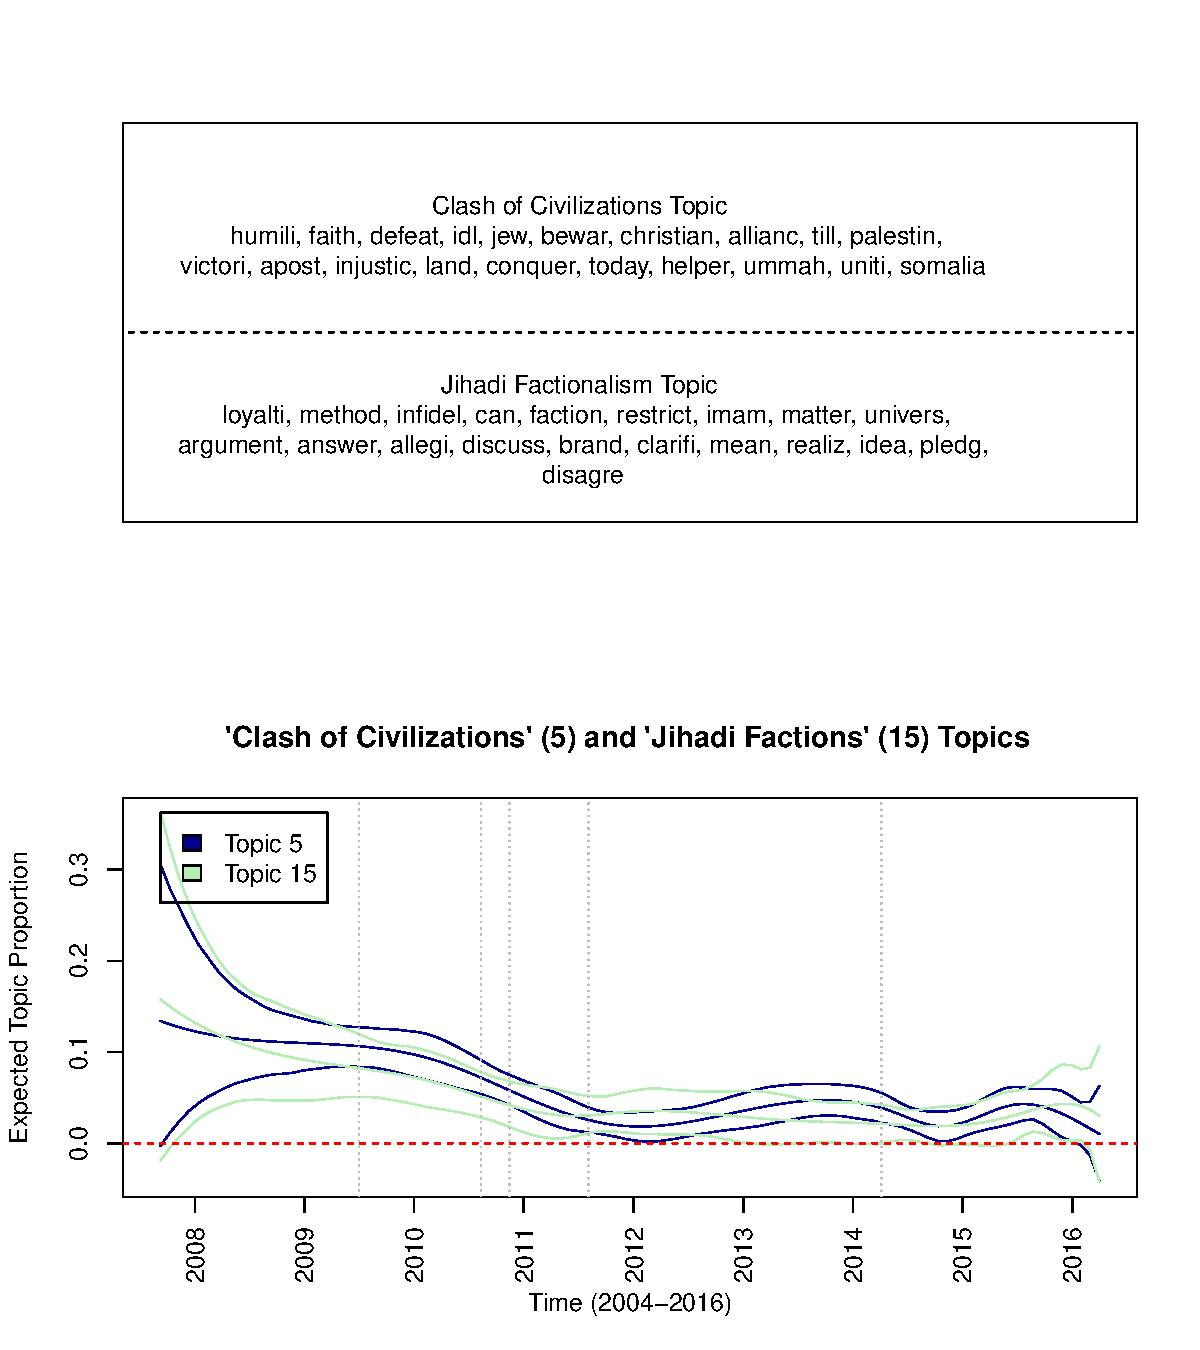
\includegraphics[width=.65\columnwidth]{./Pictures/ClashFactions_UT7_K18.pdf}\\
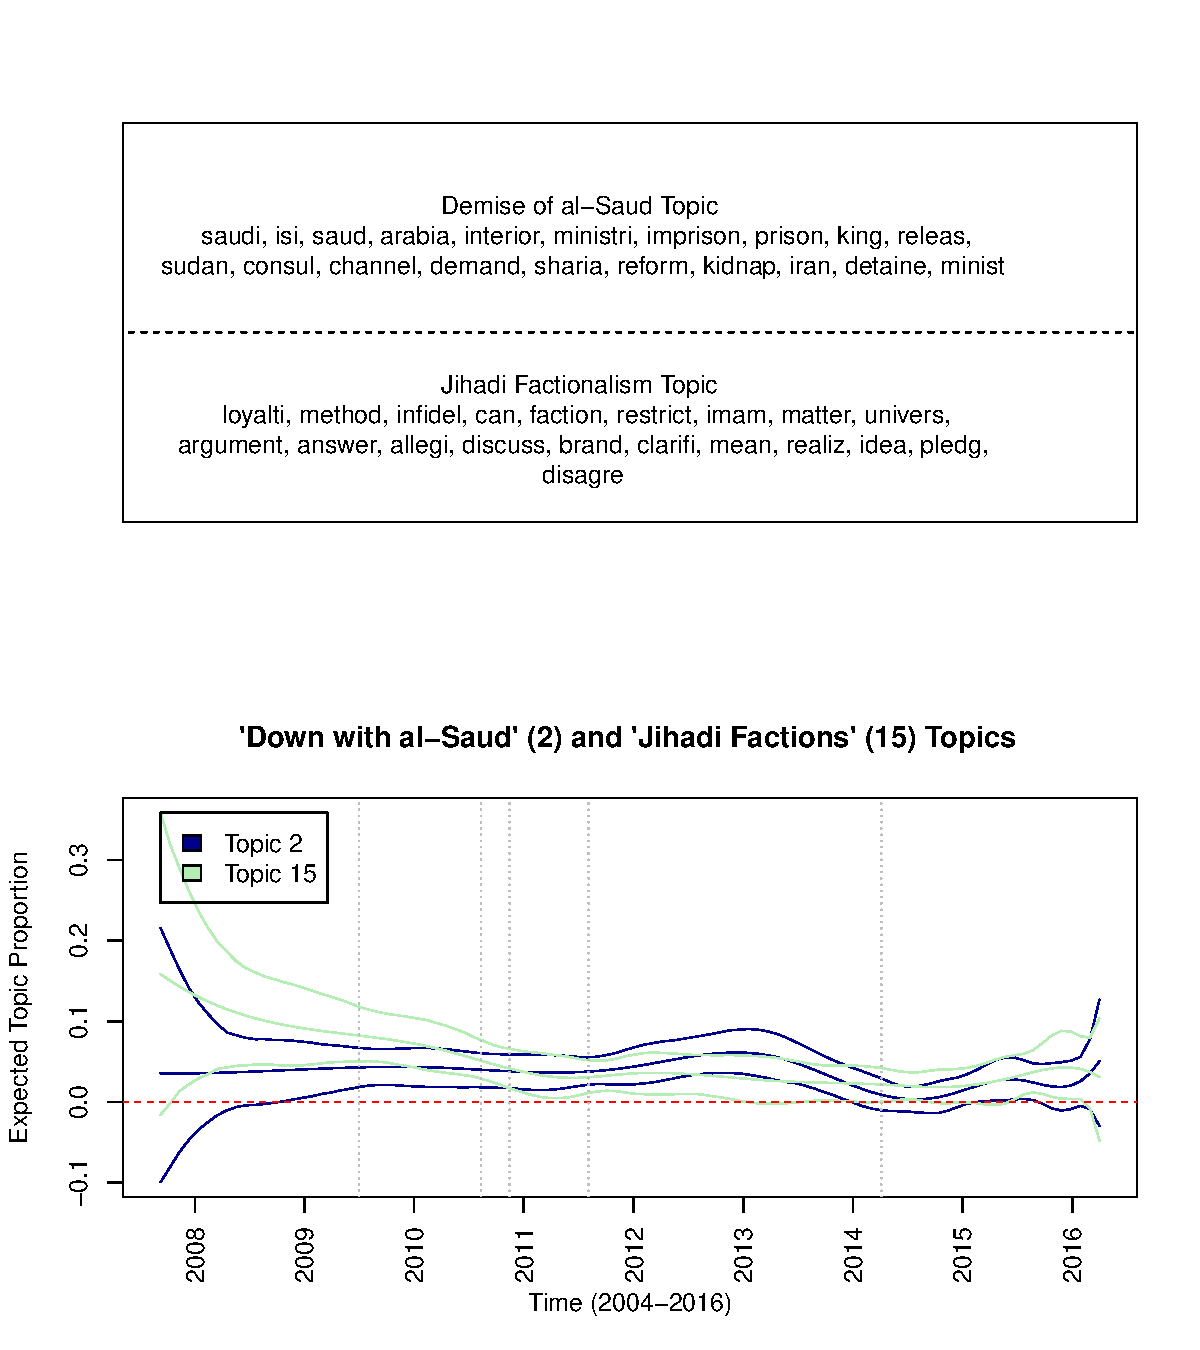
\includegraphics[width=.65\columnwidth]{./Pictures/TransJihadiAlt_UT7_K18.pdf}\\
  \end{tabular} 
\end{center}
  \end{figure*}
}
\chapter{Survey Text and Post-Processing}
\label{surveyappendix}

\section{Question Coding and Post-Processing}

This section presents the coding rules and rationale for survey post-processing.

\subsection{Mission Area}

In order to characterize survey respondents according to comparable mission areas, I clustered responses to the open-ended demographic question \say{On what mission does your organization spend the most time and money?}  Respondents provided 300 unique answers, and so I clustered the responses into comparable general and specific mission areas.

When clustering the responses, I divided up the answers into two categories: those who answered with an operational summary of the management tasks that they face and those who responded with the organization's activities.  For those that responded substantively about the mission, I clustered the responses into nine general categories: Animal Welfare, Arts and Culture, Environment, International, Domestic Social, Religious, Health, Education, Religious, and Other.  The distribution of mission types can be seen in Table~\ref{tab:clusterprops}. 
 \begin{table}[ht]
 \centering
 \begin{tabular}{rlrr}
   \hline
  & Cluster Theme & Number & Response Percentages \\
   \hline
 1 & Animal Welfare &   3 & 0.90\% \\
   2 & Arts and Culture &  12 & 3.80\% \\
   3 & Education &  18 & 5.60\%\\
   4 & Environmental &   6 & 1.90\% \\
   5 & Health &  22 & 6.90\% \\
   6 & International &   9 & 2.80\% \\
   7 & Operational & 137 & 42.90\% \\
   8 & Other &   3 & 0.90\% \\
   9 & Religious &  17 & 5.30\% \\
   10 & Social &  92 & 28.80\% \\
    \hline
 \end{tabular}
\caption{Distribution of General Mission Themes}
\label{tab:clusterprops}
 \end{table}
 
After classifying the reported mission areas, the \say{Domestic Social} and \say{Health} categories were populous enough to warrant additional subcategories. These subcategories are given in Table~\ref{tab:socmissions} and Table~\ref{tab:healthareas}

\begin{table}[ht]
\centering
 \begin{tabular}{lrr}
   \hline
  Cluster & Frequency & Percentage \\
   \hline
 Elderly and disabilities &  10 & 11.20\% \\
   Housing &  14 & 15.70\% \\
   Hunger &   5 & 5.60\% \\
   Other &  31 & 34.80\% \\
  Recreation &   3 & 3.40\% \\
    Violence\/crime &   2 & 2.20\% \\
 Vocational &   3 & 3.40\% \\
   Youth &  21 & 23.60\% \\
    \hline
 \end{tabular}
 \caption{Mission subcategories in Social Services Organizations}
 \label{tab:socmissions}
 \end{table}
 
  \begin{table}[ht]
 \centering
 \begin{tabular}{lrr}
   \hline
  Cluster & Number & Percent of Responses \\
   \hline
 Addictions &   1 & 4.50 \\
 Mental health &   4 & 18.20 \\
 Physical health &   9 & 40.90 \\
  Other &   8 & 36.40 \\
    \hline
 \end{tabular}
 \caption{Subcategories in Health Organizations}
 \label{tab:healthareas}
 \end{table}
 
In addition to substantive mission areas, approximately 40\% of the respondents listed teh  which I named broadly as \say{Operational}, staffing, finances, and outreach or expansion were common responses. After evaluating the responses, I clustered specific answers into common categories of answers in the responses. These are presented in Table~\ref{tab:activityareas}.

 \begin{table}[ht]
 \centering
 \begin{tabular}{lrr}
   \hline
 Activities & Number & Response Percentages \\
   \hline
  Administration &   2 & 1.50\% \\
    Don’t know &   8 & 5.80\% \\
   Finances &  14 & 10.20\% \\
   Growth &   9 & 6.60\% \\
  Infrastructure &   2 & 1.50\% \\
  Membership &   2 & 1.50\% \\
   Operations &  65 & 47.40\% \\
   Other &   4 & 2.90\% \\
   Outreach &  17 & 12.40\% \\
    Staffing &  14 & 10.20\% \\
    \hline
 \end{tabular}
 \caption{Clustering of Activities Described in Operational Responses}
 \label{tab:activityareas}
 \end{table}

\subsection{Question: Organization Size}

In order to identify the size of the organization that the respondents worked within, the survey asked respondents \say{What is the approximate number of people in your organization?}. After converting the free-text answer into an integer, I clustered the answers into seven bins ranging, from 0-2 to over 100 people. The bin sizes increase as the number of reported personnel increases, with three bins for a size of less than 10, and then one for 11-20, one for 21-50, one for 51-100, and one for any reporting over 100. The rationale for this categorization is twofold: the reported sizes exhibits a long tail, with over 200 of the 298 responses reporting a size of less than 10 people. The distribution of reported personnel sizes for those organizations reporting 100 or fewer people in the organization is displayed in Figure~\ref{fig:censoredsizes}.

%% Here put the box plot of size (and then one zoomed in)

\begin{table}
\centering
\begin{tabular}{cc}
    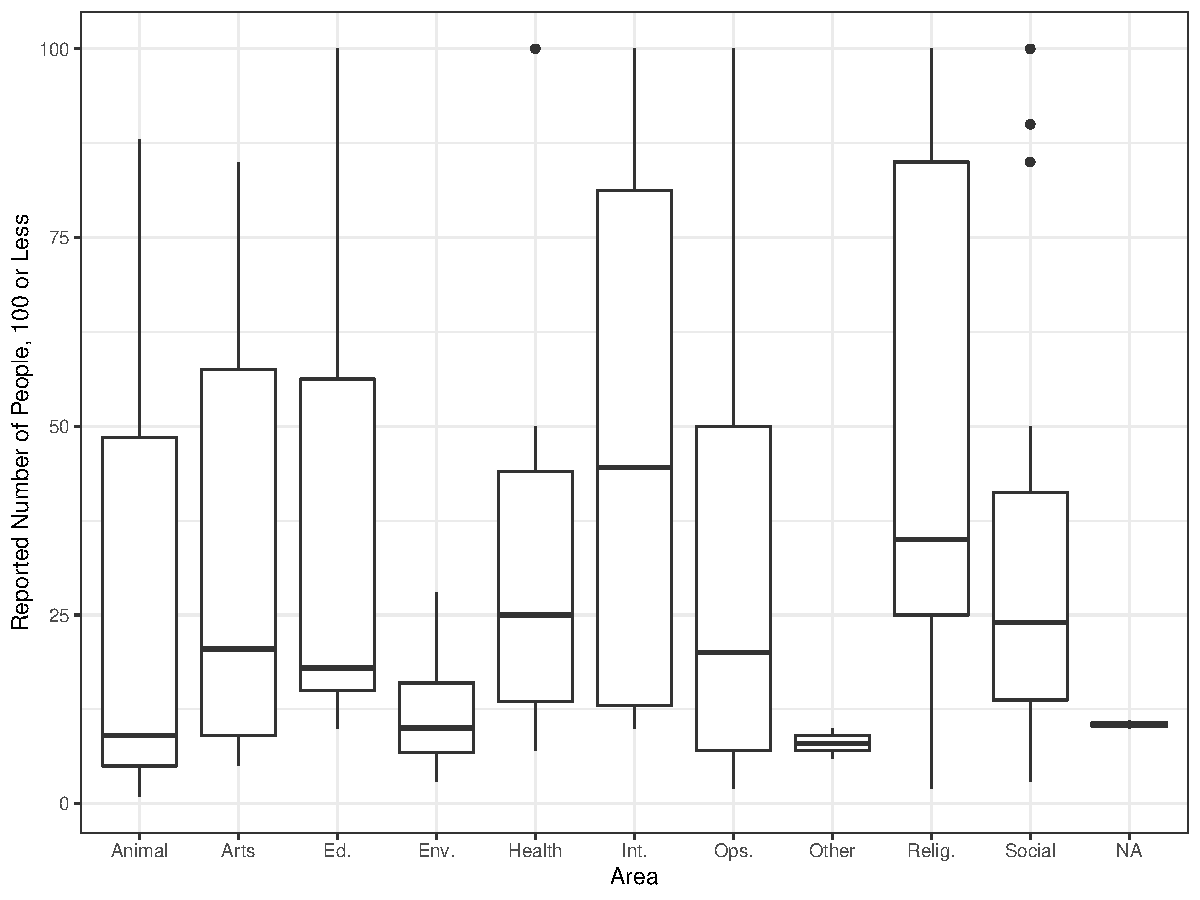
\includegraphics[width=.45\columnwidth]{./Pictures/censoredsizebysector.pdf}
&
    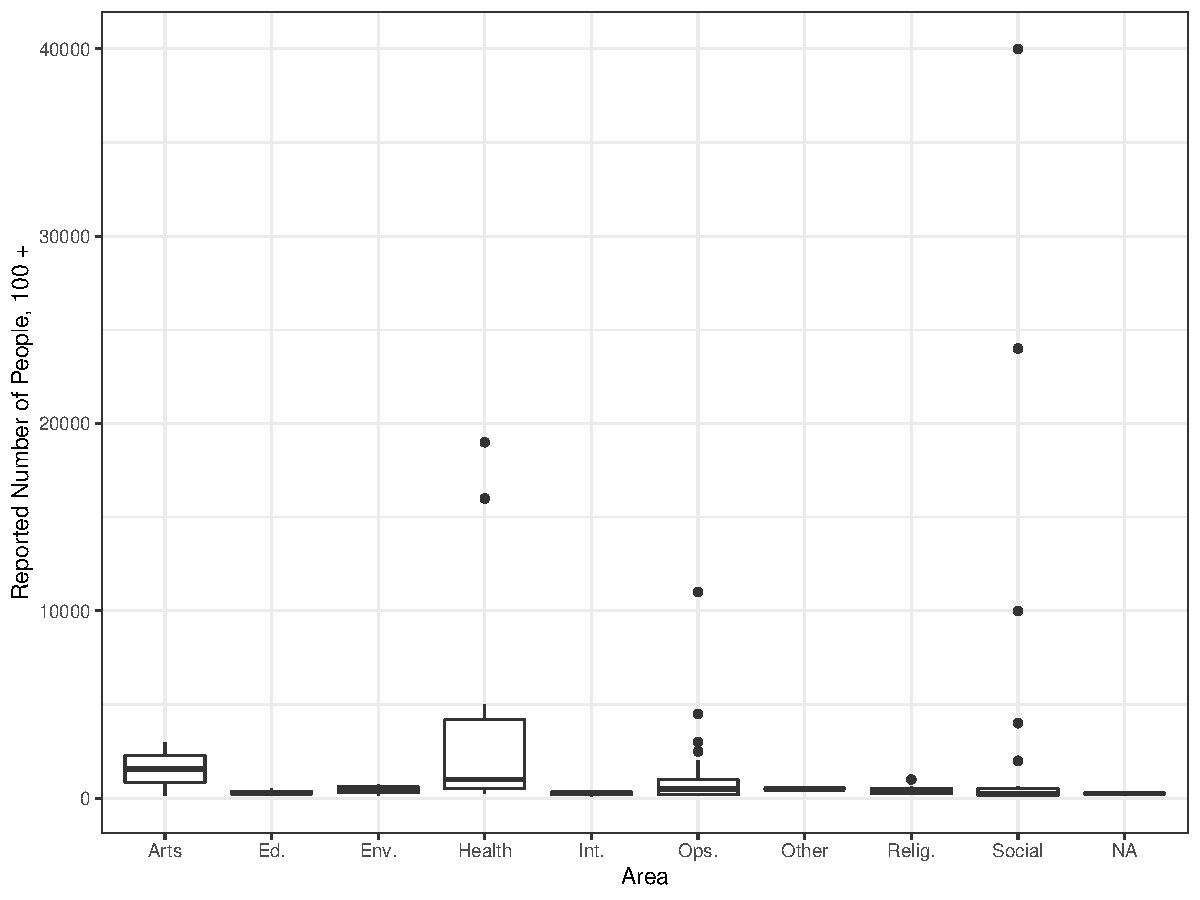
\includegraphics[width=.45\columnwidth]{./Pictures/censoredsizebysectorbig.pdf}
\\
Size $\leq$ 100 &  Size $> 100 $ \\
\end{tabular}
    \caption{Distribution of Reported Personnel Sizes}
    \label{fig:censoredsizes}
\end{table}



The expectation that smaller organizations would have less bandwidth to absorb a large influx of new staff also informed the decision to summarize the results with a more precise focus on smaller organizations.

It is more common for surveys of non-profits to classify size of the non-profit according to the size of the operating budget. Instead of following this format, the survey asked for personnel size because the project is interested in rapid staff expansions. Despite the difference in substantive focus, budget and the number of full-time employees are strongly correlated~\autocite{carman2009nonprofits}.  

\subsection{Descriptions of Origin of Post-Expansion Mission Drift}

In order to estimate the overall frequency of expansion-driven change among the non-profit respondents, the survey posed a three part question. The sequence began with the question: \say{Have you have ever been part of an organization experiencing a period of rapid growth or personnel change among the staff or the board of directors?}. The distribution of responses reporting a rapid staff growth are displayed in Figure~\ref{fig:q13staffsummary} For those who responded in the affirmative, the survey asked the follow-up question: \say{Did you feel that the personnel changes contributed to mission drift or other strategic changes?}. The result of the question, disaggregated by reported size and clustered mission area are shown in Figure~\ref{fig:q14summary}. Finally, the survey asked for open-ended reflection on where the respondent believed that the changes originated. The question asked: \say{In a sentence or two, can you describe where the changes originated?} 

\begin{figure}
\centering
    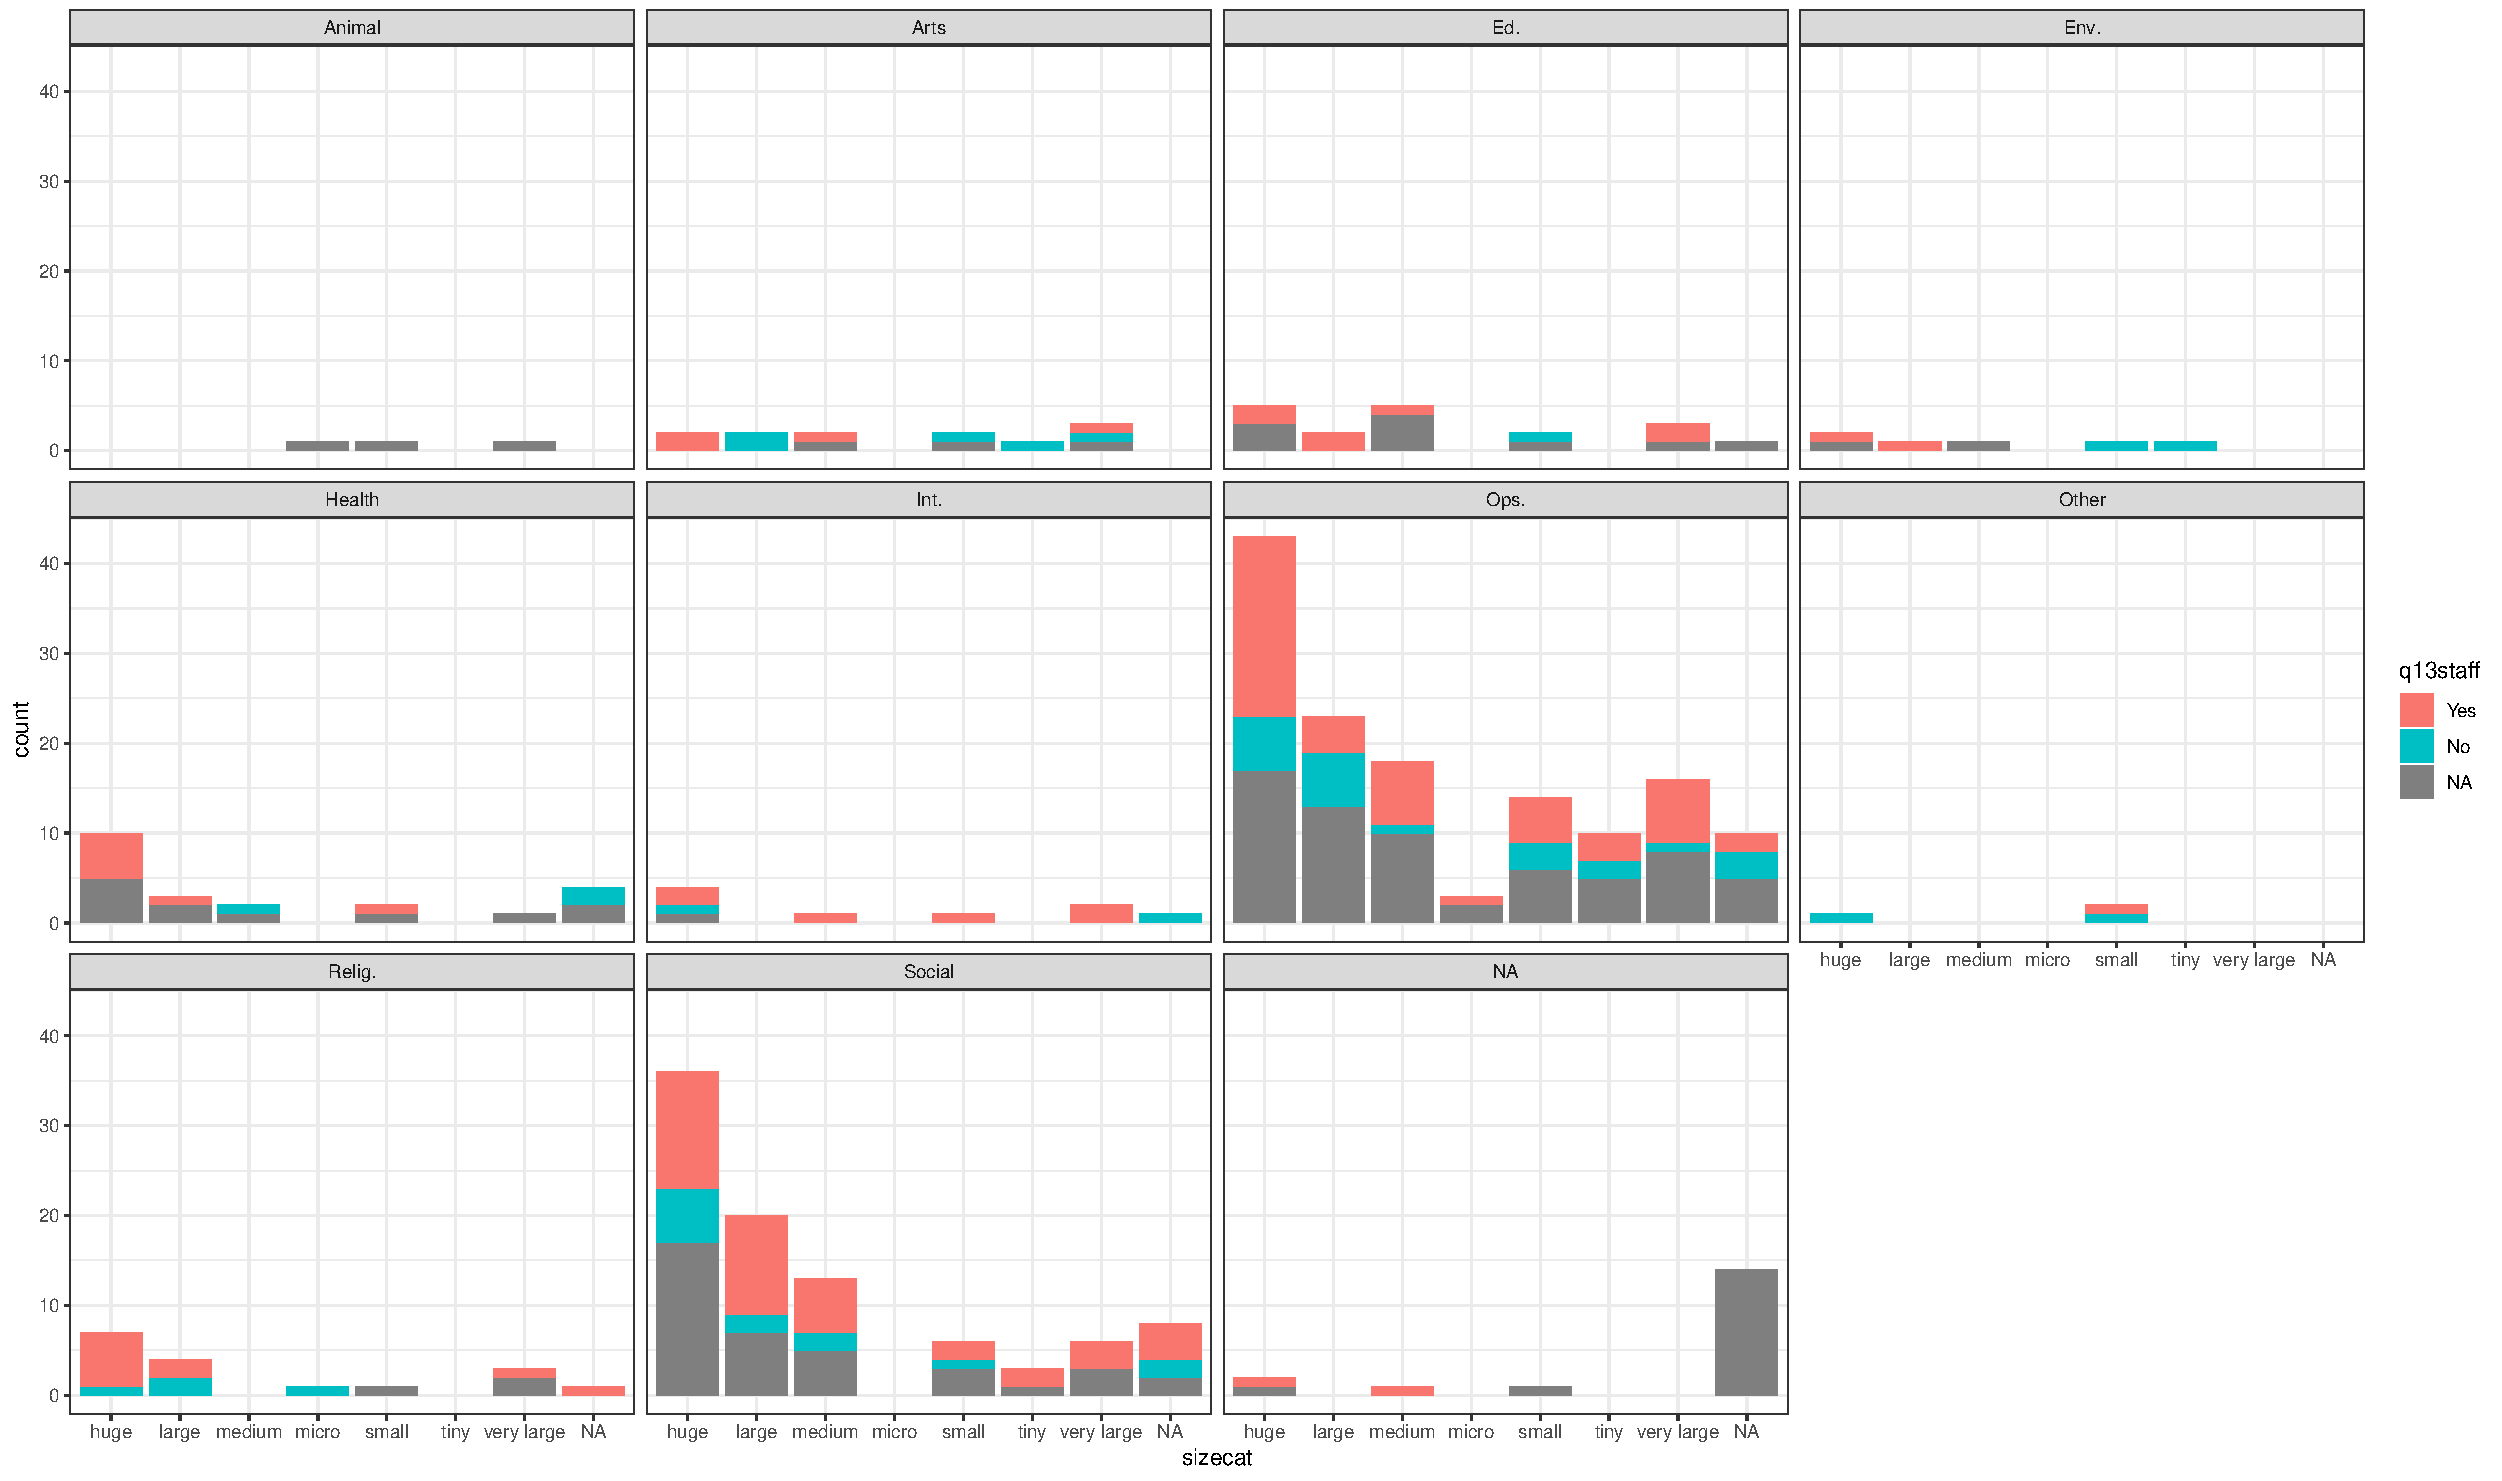
\includegraphics[width=.85\columnwidth]{./Pictures/rapidstaffgrowthbysizeandsector.pdf}
    \caption{Reports of Rapid Staff Expansion, By Size Category and Mission Cluster}
    \label{fig:q13staffsummary}
\end{figure}


\begin{figure}
\centering
    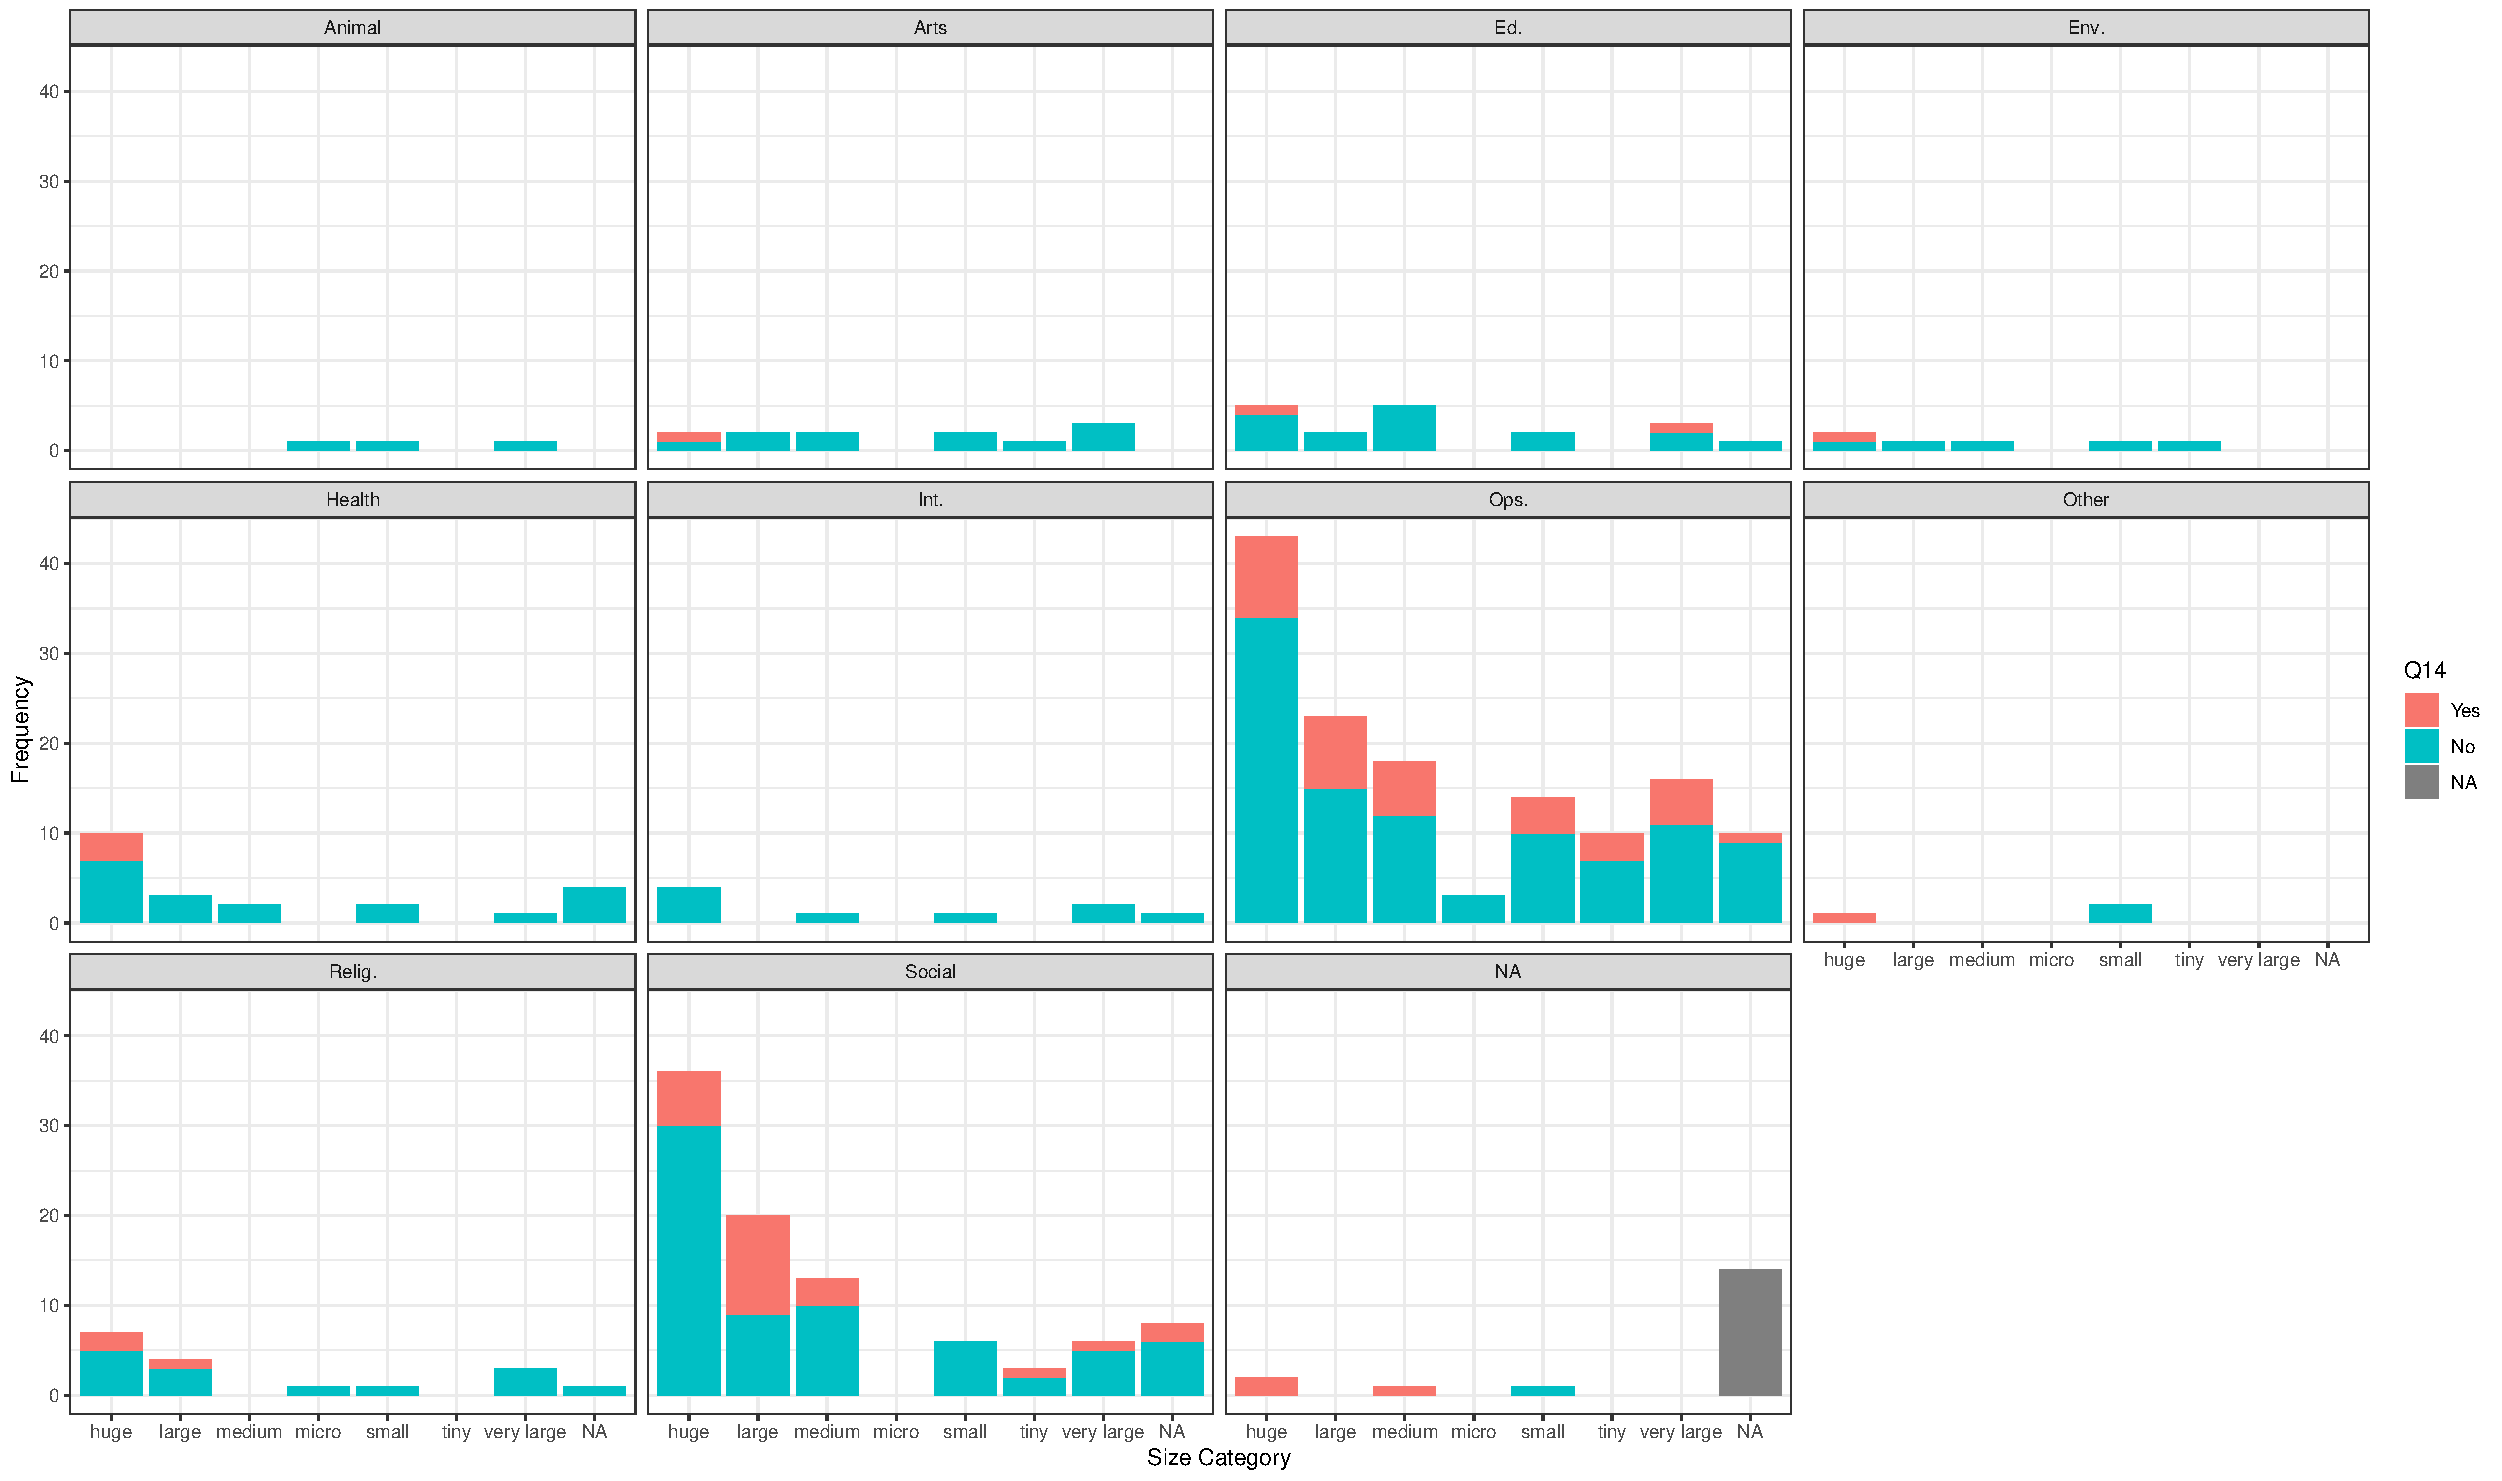
\includegraphics[width=.85\columnwidth]{./Pictures/missiondriftaftergrowth.pdf}
    \caption{Reports of Mission Drift After Rapid Growth, By Size Category and Mission Cluster}
    \label{fig:q14summary}
\end{figure}
% summary of yeses by mission category for question 13; 14; 

For the analysis, I standardized the responses, clustering them into seven general categories: no change reported; change originating from the top-down with the Board of Directors, executive officers, or general leaders;  change originating from the bottom-up and instigated by staff; change motivated by shifting demographics of the membership base or in the services provided; change originating from financial necessity; and a general category for an origin of change that did not fall into the existing categories. Finally, two residual categories noted, respectively, a cluster of answers that described a tactical motivator for change, and another in which respondents reported a technical glitch in the survey flow.\footnote{These responses were removed from the series of questions about expansion and subsequent change, so that the platform problem did not influence overall results.}

%% summary of some of the free text answers in question 16

\subsection{Descriptions of Result of Short-Term Changes}  

The bottom-up transformation theory rests on a claim that even strategic leaders can be induced to downplay long-term best practices in favor of a short-term gain or advantage. To provide an empirical basis for this assertion, the survey asked respondents \say{Have the leaders of your organization ever decided to strengthen the morale and cohesion of your organization in the short-term, even if the decision might influence the long-term strategy?} For those who answered in the affirmative, the survey provided an open-ended followup question: \say{In a sentence or two, can you describe the result of this decision?}

To standardize the responses for analysis, I clustered the free-responses into five general outcomes. The substantive clusters classified responses into whether they reported a positive or negative outcome. Reported positive outcomes frequently described reinvigorated staff, better recruiting, and a recommitment to the original mission. Conversely, the negative responses gathered responses that reported leaders pushed out or resigning, mission drift, disconnects between leaders and the base, and an overall reduction in quality of staff or services.  A  third cluster of responses indicated that they were still experiencing the fallout of the short-term changes, and so were unable to report yet. Finally, the three residual categories collected responses that indicated that the respondent had not experienced that type of outcome; did not know the results or understand the question; or that they shared advice for managing morale or retrenching against mission drift.

\section{Additional Graphs from Conjoint Experiment}

The conjoint experiment posed two hypothetical hiring scenarios to survey respondents, asking them to compare which of two candidates for a staff and a Board of Directors position they would prefer to hire. For both vignettes, the candidates were named \say{Candidate A} and \say{Candidate B,} with \say{Candidate A} being the option with varying traits.

The staff recruitment vignette presented respondents with the prompt:

\begin{quote}
Imagine you are recruiting new staff for a hypothetical organization similar to your own. The organization's funding is: \textit{{[Resource Condition]}}
There are two groups of equally well-qualified candidates:\\
Candidates in \textbf{Group A} have a mission that is \textit{{[Agreement Condition]}} the organization's mission. You expect that if they join, they will try to steer the organization's mission to align with their goals. However, there is a large foundation running a fellowship program that will subsidize their salary and benefits at \textit{{[Subsidy Condition]}}\\
Candidates in \textbf{Group B} share a mission with the organization. They are not eligible for the subsidy, and so their salary and benefits will be borne solely by the organization.\\
The candidate profiles are summarized below.\\
Drawing from your professional experience, from which group of candidates would you prefer to recruit staff?
\end{quote}

Respondents were then presented with a Board member recruitment vignette, which asked them to engage with the following scenario:

\begin{quote}
Now imagine you are recruiting a new board member for an organization similar to your own. The organization's funding is: \textit{{[Resource Condition]}}
There are two equally well-qualified candidates for the board:\\

\textbf{Candidate 1}: prefers a mission that is \textit{{[Agreement Condition]}} the organization that is seeking a board member.  The candidate \textit{{[Skills Condition]}} bring new professional skills that the board needs. You expect that if they join the board, they will try to steer the organization towards their mission.

\textbf{Candidate 2}: shares the same mission as the organization and so you do not expect them to try to change the organization's mission. They will not bring new professional skills to the board.\\
Which of the two candidates would you prefer to have on the board of directors?
\end{quote}

As Figure~\ref{fig:traitssector} indicates, the respondents largely responded similarly regardless of the sector or type of mission that they reported engaging in. Those respondents reporting activity in the \say{social} sector were the most averse to candidates with divergent preferences. But, otherwise, the response patterns are broadly similar, and therefore the responses were analyzed without differentiating the reported mission.

\begin{figure}
\centering
    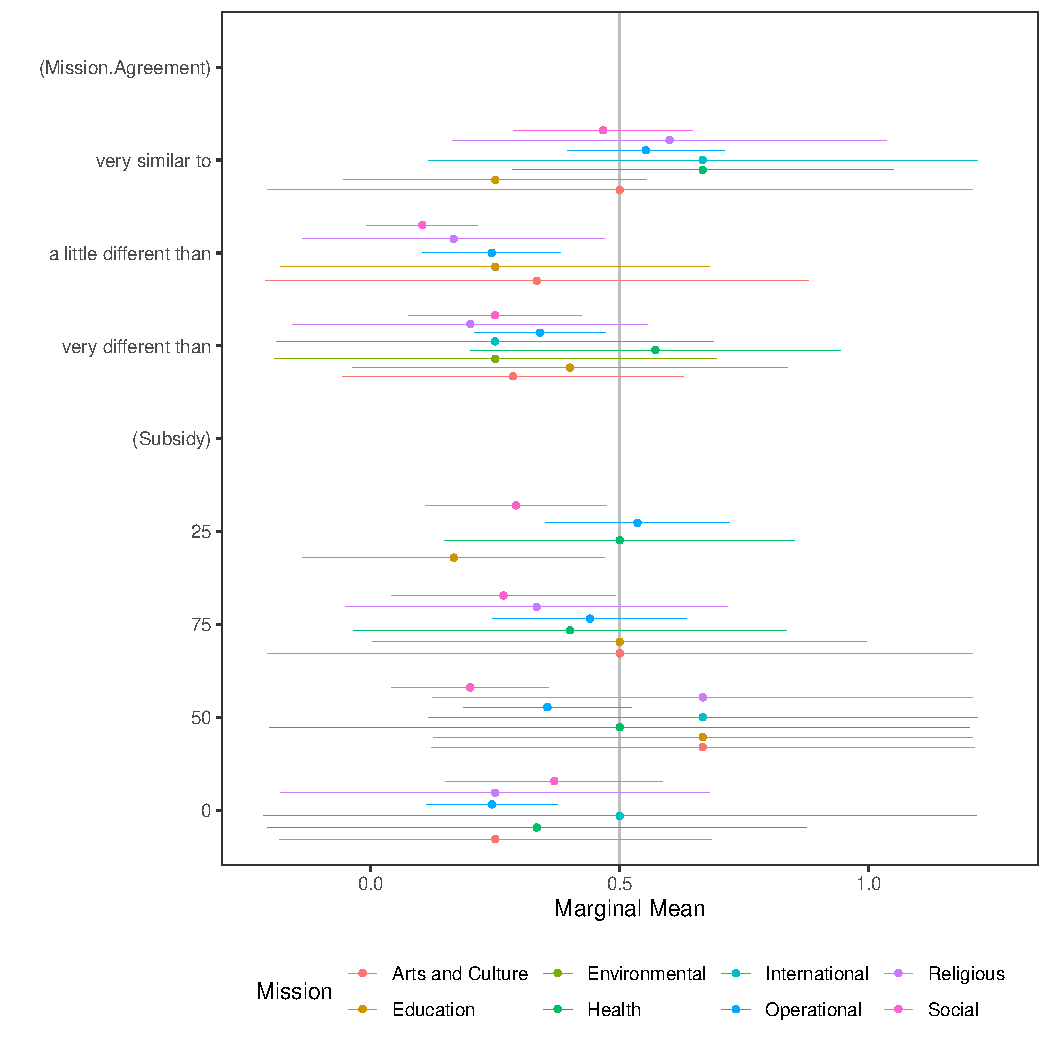
\includegraphics[width=.95\columnwidth]{./Pictures/traitsBySector.pdf}
    \caption{Trait Attractiveness By Respondent Sector}
    \label{fig:traitssector}
\end{figure}

Estimating the Average Marginal Effects by looping over the feature levels for each possible reference category for the candidate traits indicates that the estimated outcome is not sensitive to the choice of reference category. Indeed, the results of the sensitivity analysis, shown in Figure~\ref{fig:acmesens} are consistent with the overall takeaway that conjoint survey participants paid most attention to mission alignment.


\begin{figure}
\centering
    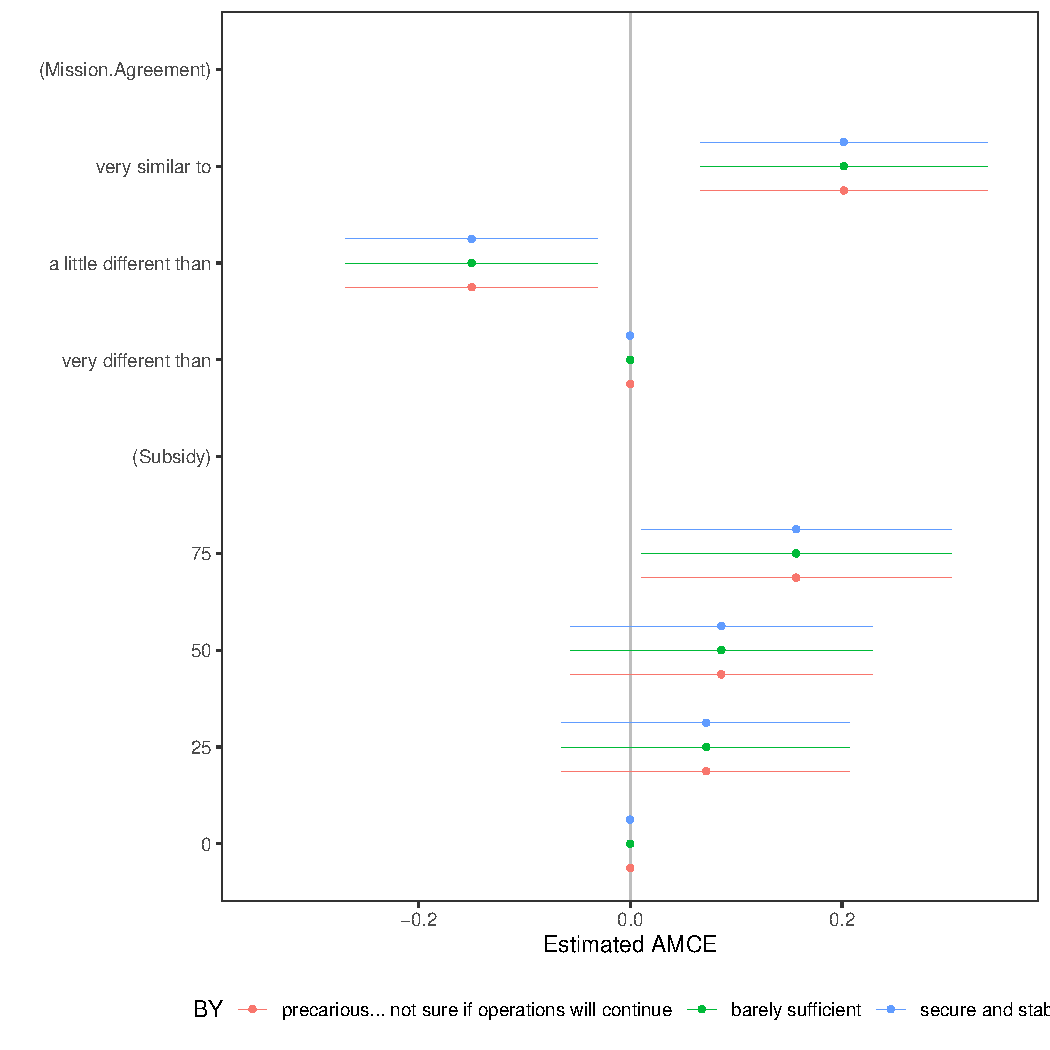
\includegraphics[width=.95\columnwidth]{./Pictures/acmeSensitivity.pdf}
    \caption{ACME Sensitivity Plot}
    \label{fig:acmesens}
\end{figure}


%% summaries of the classification for Q21.

}
%-----------------------------------------------------------------------------%
% BIBLIOGRAPHY -- uncomment \nocite{*} to include items in 'mybib.bib' file
% that aren't cited in the text.  Change the style to match your
% discipline's standards.  Of course, if your bibliography file isn't called
% 'mybib.bib' you might want to change that here too :)
%-----------------------------------------------------------------------------%
%\nocite{*} - if you use this it will put EVERYTHING in your .bib file into the references even if you don't cite it in the text
%\bibliographystyle{./Bibliography/apsr2006} %Formats bibliography
\cleardoublepage
\begingroup
\setstretch{1.0}
\addcontentsline{toc}{chapter}{Bibliography} %adds Bibliography to your table of contents
\printbibliography
\endgroup

%\normalbaselines %Fixes spacing of bibliography

%\printbibliography %% Prints using the biblatex package, not the natbib originally with the package
%-----------------------------------------------------------------------------%

%-----------------------------------------------------------------------------%
% BIOGRAPHY -- Start file with '\biography'.  Mandatory for Ph.D.
%-----------------------------------------------------------------------------%
%\biography
Your biography is limited to one page and must contain
\begin{enumerate}
\normalbaselines
\item Full name
\item Date and place of birth
\item Every degree you've earned, including this one, and where you earned it
      from.
\end{enumerate}
Mostly, that information is to narrow down which John Smith wrote that
dissertation on the mating habits of sea cucumbers.  Sexy!

You may also include
\begin{enumerate}
\item Any awards you've won related to your discipline since your
undergraduate degree.
\item Any fellowships you've held
\item Anything you've published (papers, books, book chapters).  Don't be
afraid to cite it here, so that the full bibliographic record of your
article appears in the bibliography!
\item Where your next job will be, if you know
\end{enumerate}



}

%-----------------------------------------------------------------------------
% You're done :)
\end{document}
